% Options for packages loaded elsewhere
\PassOptionsToPackage{unicode}{hyperref}
\PassOptionsToPackage{hyphens}{url}
%
\documentclass[
]{book}
\usepackage{amsmath,amssymb}
\usepackage{iftex}
\ifPDFTeX
  \usepackage[T1]{fontenc}
  \usepackage[utf8]{inputenc}
  \usepackage{textcomp} % provide euro and other symbols
\else % if luatex or xetex
  \usepackage{unicode-math} % this also loads fontspec
  \defaultfontfeatures{Scale=MatchLowercase}
  \defaultfontfeatures[\rmfamily]{Ligatures=TeX,Scale=1}
\fi
\usepackage{lmodern}
\ifPDFTeX\else
  % xetex/luatex font selection
\fi
% Use upquote if available, for straight quotes in verbatim environments
\IfFileExists{upquote.sty}{\usepackage{upquote}}{}
\IfFileExists{microtype.sty}{% use microtype if available
  \usepackage[]{microtype}
  \UseMicrotypeSet[protrusion]{basicmath} % disable protrusion for tt fonts
}{}
\makeatletter
\@ifundefined{KOMAClassName}{% if non-KOMA class
  \IfFileExists{parskip.sty}{%
    \usepackage{parskip}
  }{% else
    \setlength{\parindent}{0pt}
    \setlength{\parskip}{6pt plus 2pt minus 1pt}}
}{% if KOMA class
  \KOMAoptions{parskip=half}}
\makeatother
\usepackage{xcolor}
\usepackage{color}
\usepackage{fancyvrb}
\newcommand{\VerbBar}{|}
\newcommand{\VERB}{\Verb[commandchars=\\\{\}]}
\DefineVerbatimEnvironment{Highlighting}{Verbatim}{commandchars=\\\{\}}
% Add ',fontsize=\small' for more characters per line
\usepackage{framed}
\definecolor{shadecolor}{RGB}{248,248,248}
\newenvironment{Shaded}{\begin{snugshade}}{\end{snugshade}}
\newcommand{\AlertTok}[1]{\textcolor[rgb]{0.94,0.16,0.16}{#1}}
\newcommand{\AnnotationTok}[1]{\textcolor[rgb]{0.56,0.35,0.01}{\textbf{\textit{#1}}}}
\newcommand{\AttributeTok}[1]{\textcolor[rgb]{0.13,0.29,0.53}{#1}}
\newcommand{\BaseNTok}[1]{\textcolor[rgb]{0.00,0.00,0.81}{#1}}
\newcommand{\BuiltInTok}[1]{#1}
\newcommand{\CharTok}[1]{\textcolor[rgb]{0.31,0.60,0.02}{#1}}
\newcommand{\CommentTok}[1]{\textcolor[rgb]{0.56,0.35,0.01}{\textit{#1}}}
\newcommand{\CommentVarTok}[1]{\textcolor[rgb]{0.56,0.35,0.01}{\textbf{\textit{#1}}}}
\newcommand{\ConstantTok}[1]{\textcolor[rgb]{0.56,0.35,0.01}{#1}}
\newcommand{\ControlFlowTok}[1]{\textcolor[rgb]{0.13,0.29,0.53}{\textbf{#1}}}
\newcommand{\DataTypeTok}[1]{\textcolor[rgb]{0.13,0.29,0.53}{#1}}
\newcommand{\DecValTok}[1]{\textcolor[rgb]{0.00,0.00,0.81}{#1}}
\newcommand{\DocumentationTok}[1]{\textcolor[rgb]{0.56,0.35,0.01}{\textbf{\textit{#1}}}}
\newcommand{\ErrorTok}[1]{\textcolor[rgb]{0.64,0.00,0.00}{\textbf{#1}}}
\newcommand{\ExtensionTok}[1]{#1}
\newcommand{\FloatTok}[1]{\textcolor[rgb]{0.00,0.00,0.81}{#1}}
\newcommand{\FunctionTok}[1]{\textcolor[rgb]{0.13,0.29,0.53}{\textbf{#1}}}
\newcommand{\ImportTok}[1]{#1}
\newcommand{\InformationTok}[1]{\textcolor[rgb]{0.56,0.35,0.01}{\textbf{\textit{#1}}}}
\newcommand{\KeywordTok}[1]{\textcolor[rgb]{0.13,0.29,0.53}{\textbf{#1}}}
\newcommand{\NormalTok}[1]{#1}
\newcommand{\OperatorTok}[1]{\textcolor[rgb]{0.81,0.36,0.00}{\textbf{#1}}}
\newcommand{\OtherTok}[1]{\textcolor[rgb]{0.56,0.35,0.01}{#1}}
\newcommand{\PreprocessorTok}[1]{\textcolor[rgb]{0.56,0.35,0.01}{\textit{#1}}}
\newcommand{\RegionMarkerTok}[1]{#1}
\newcommand{\SpecialCharTok}[1]{\textcolor[rgb]{0.81,0.36,0.00}{\textbf{#1}}}
\newcommand{\SpecialStringTok}[1]{\textcolor[rgb]{0.31,0.60,0.02}{#1}}
\newcommand{\StringTok}[1]{\textcolor[rgb]{0.31,0.60,0.02}{#1}}
\newcommand{\VariableTok}[1]{\textcolor[rgb]{0.00,0.00,0.00}{#1}}
\newcommand{\VerbatimStringTok}[1]{\textcolor[rgb]{0.31,0.60,0.02}{#1}}
\newcommand{\WarningTok}[1]{\textcolor[rgb]{0.56,0.35,0.01}{\textbf{\textit{#1}}}}
\usepackage{longtable,booktabs,array}
\usepackage{calc} % for calculating minipage widths
% Correct order of tables after \paragraph or \subparagraph
\usepackage{etoolbox}
\makeatletter
\patchcmd\longtable{\par}{\if@noskipsec\mbox{}\fi\par}{}{}
\makeatother
% Allow footnotes in longtable head/foot
\IfFileExists{footnotehyper.sty}{\usepackage{footnotehyper}}{\usepackage{footnote}}
\makesavenoteenv{longtable}
\usepackage{graphicx}
\makeatletter
\def\maxwidth{\ifdim\Gin@nat@width>\linewidth\linewidth\else\Gin@nat@width\fi}
\def\maxheight{\ifdim\Gin@nat@height>\textheight\textheight\else\Gin@nat@height\fi}
\makeatother
% Scale images if necessary, so that they will not overflow the page
% margins by default, and it is still possible to overwrite the defaults
% using explicit options in \includegraphics[width, height, ...]{}
\setkeys{Gin}{width=\maxwidth,height=\maxheight,keepaspectratio}
% Set default figure placement to htbp
\makeatletter
\def\fps@figure{htbp}
\makeatother
\setlength{\emergencystretch}{3em} % prevent overfull lines
\providecommand{\tightlist}{%
  \setlength{\itemsep}{0pt}\setlength{\parskip}{0pt}}
\setcounter{secnumdepth}{5}
\usepackage{booktabs}
\usepackage{amsthm}
\makeatletter
\def\thm@space@setup{%
  \thm@preskip=8pt plus 2pt minus 4pt
  \thm@postskip=\thm@preskip
}
\makeatother
\ifLuaTeX
  \usepackage{selnolig}  % disable illegal ligatures
\fi
\usepackage[]{natbib}
\bibliographystyle{apalike}
\IfFileExists{bookmark.sty}{\usepackage{bookmark}}{\usepackage{hyperref}}
\IfFileExists{xurl.sty}{\usepackage{xurl}}{} % add URL line breaks if available
\urlstyle{same}
\hypersetup{
  pdftitle={Answering questions with data: Lab Manual},
  pdfauthor={Matthew J. C. Crump, Anjali Krishnan, Stephen Volz, and Alla Chavarga; Adapted for PSYC 292, St.~Francis Xavier University, by Erin L. Mazerolle, Sherry Neville-MacLean, Christine D. Lomore, and Margaret Vail.},
  hidelinks,
  pdfcreator={LaTeX via pandoc}}

\title{Answering questions with data: Lab Manual}
\author{Matthew J. C. Crump, Anjali Krishnan, Stephen Volz, and Alla Chavarga \and Adapted for PSYC 292, St.~Francis Xavier University, by Erin L. Mazerolle, Sherry Neville-MacLean, Christine D. Lomore, and Margaret Vail.}
\date{Last Compiled 2024-09-22}

\begin{document}
\maketitle

{
\setcounter{tocdepth}{1}
\tableofcontents
}
\hypertarget{preface}{%
\chapter*{Preface}\label{preface}}
\addcontentsline{toc}{chapter}{Preface}

This is the companion lab to our free introductory statistics for undergraduates in psychology textbook, \href{https://www.erinmazerolle.com/statistics/}{Answering questions with data}.

This lab manual involves step by-step tutorials to solve data analysis problems in software. We use open-data sets that are usually paired with a primary research article.

Each lab has a separate guide for solving the problems in R \& R-studio, Excel, SPSS, and JAMOVI.

The manual is a free and open resource. See below for more information about copying, making change, or contributing to the lab manual.

\hypertarget{important-notes}{%
\section{Important notes}\label{important-notes}}

This lab manual is released under a creative commons licence \href{https://creativecommons.org/licenses/by-sa/4.0/}{CC BY-SA 4.0}. Click the link to read more about the license, or read more below in the license section.

This lab manual is part of a larger OER course package for teaching undergraduate statistics in Psychology. Team members include, Matthew Crump, Alla Chavarga, Anjali Krishnan, Jeffrey Suzuki, and Stephen Volz. As this OER comes together, we will be providing a \href{https://crumplab.github.io/psyc3400/}{course website}, written in R Markdown, as well as slide decks for the lectures (these will be more fully available by the end of fall 2018). As a result, this textbook, the lab manual, the course website, and the slide decks will all be free, under a creative commons license. The source code for all material is contained in the GitHub repositories for each, and they are a written in R-markdown, so they are relatively easy to copy and edit. Have Fun!

\hypertarget{attributions-and-versions}{%
\subsection{Attributions and Versions}\label{attributions-and-versions}}

\textbf{First Draft (version 0.9 = August 15th, 2018)}

This was the version we used to adapt the lab manual. That project can be found \href{https://crumplab.github.io/statisticsLab/}{here}. It was authored by Matt Crump (R exercises), Anjali Krishnan (JAMOVI exercises), Stephen Volz (EXCEL exercises), and Alla Chavarga (SPSS exercises). Labs 6, 7, and 8 were adapted and expanded from \href{https://sites.trinity.edu/osl}{Open Stats Labs}. Thanks to Open Stats Labs (Dr.~Kevin P. McIntyre) for their fantastic work.

\textbf{Version 1.0 = April, 2021}

This version was our first edit of the lab manual for PSYC 292 at StFX (Winter 2021), and was completed by Erin Mazerolle and Sherry Neville-MacLean. The changes were mainly focused on the SPSS sections of Labs 1, 2, 3, 6, and 7, and in particular, the homework questions. We also added Lab 12.

\textbf{In progress: Version 2.0.} Last Compiled: 2024-09-22

We are currently working on updating the lab manual to include JAMOVI activities that will use in PSYC 292 at StFX.

Section 0.6 of Lab 0 was adapted nearly verbatim, with some editorial changes, from Chapter 3, ``Getting started with jamovi,'' from Navarro, D.J., \& Foxcroft, D.R. (2019). Learning statistics with jamovi: A tutorial for psychology students and other beginners. (Version 0.70) while adhering to its license that states ``The book is released under a creative commons CC BY-SA 4.0 licence. This means that this book can be reused, remixed, retained, revised and redistributed (including commercially) as long as appropriate credit is given to the authors. If you remix, or modify the original version of this open textbook, you must redistribute all versions of this open textbook under the same license - \href{https://creativecommons.org/licenses/by-sa/4.0/deed.ast}{CC BY-SA}. DOI: 10.24384/hgc3-7p15

\hypertarget{cc-by-sa-4.0-license}{%
\subsection{CC BY-SA 4.0 license}\label{cc-by-sa-4.0-license}}

This license means that you are free to:

\begin{itemize}
\tightlist
\item
  Share: copy and redistribute the material in any medium or format
\item
  Adapt: remix, transform, and build upon the material for any purpose, even commercially.
\end{itemize}

The licensor cannot revoke these freedoms as long as you follow the license terms.

Under the following terms:

\begin{itemize}
\tightlist
\item
  Attribution: You must give appropriate credit, provide a link to the license, and indicate if changes were made. You may do so in any reasonable manner, but not in any way that suggests the licensor endorses you or your use.
\item
  ShareAlike: If you remix, transform, or build upon the material, you must distribute your contributions under the same license as the original.
\item
  No additional restrictions: You may not apply legal terms or technological measures that legally restrict others from doing anything the license permits.
\end{itemize}

\hypertarget{copying-the-lab-manual}{%
\subsection{Copying the lab manual}\label{copying-the-lab-manual}}

This lab manual was written in R-Studio, using R Markdown, and compiled into a web-book format using the bookdown package.

All of the source code for this book is available in a GitHub repository: \url{https://github.com/erinmaz/statisticsLab}

In addition, the source code for project this book was based on can be found at: \url{https://github.com/CrumpLab/statisticsLab}

In principle, anybody could fork or otherwise download this repository. Load the Rproj file in R-studio, and then compile the entire book. Then, the individual .rmd files for each chapter could be edited for content and style to better suit your needs.

If you want to contribute to this version of the lab manual, you could make pull requests on GitHub, or discuss issues and request on the issues tab.

\hypertarget{acknowledgments}{%
\subsection{Acknowledgments}\label{acknowledgments}}

Thanks to the librarians at Brooklyn College of CUNY, especially Miriam Deutch, and Emily Fairey, for their support throughout the process. Thanks to CUNY for supporting OER development, and for the grant we received to develop this work.

Development of version 2.0 (described above) was funded by the \href{https://www.caul-cbua.ca/}{Council of Atlantic University Libraries} through an AtlanticOER Development Grant awarded to Erin Mazerolle, Christine Lomore, Margaret Vail, Derrick Lee, Sherry Neville-MacLean, and Lindsay Berrigan.

\hypertarget{software}{%
\chapter*{Software}\label{software}}
\addcontentsline{toc}{chapter}{Software}

\hypertarget{data}{%
\section{Data}\label{data}}

Data files used for the labs are all taken from open data sources. Links are provided for each lab. For convenience, all of the data files are also available here as single files in the github repository for this lab manual

\hypertarget{data-repository}{%
\subsection{Data Repository}\label{data-repository}}

\url{https://github.com/CrumpLab/statisticsLab/tree/master/data}

\hypertarget{csv-format}{%
\subsection{CSV format}\label{csv-format}}

All of the data files in .csv format are also available to \href{https://raw.githubusercontent.com/CrumpLab/statisticsLab/master/data/data_csv.zip}{download as a .zip file}

\hypertarget{spss-format}{%
\subsection{SPSS format}\label{spss-format}}

All of the data files in SPSS format are also available to \href{https://raw.githubusercontent.com/CrumpLab/statisticsLab/master/data/spssdata/spss_data.zip}{download as a .zip file}

\hypertarget{r}{%
\section{R}\label{r}}

\includegraphics{figures/rlogo.jpg}

In this course we will be using R as a tool to analyze data, and as a tool to help us gain a better understanding of what our analyses are doing. Throughout each lab we will show you how to use R to solve specific problems, and then you will use the examples to solve homework and lab assignments. R is a very deep programming language, and in many ways we will only be skimming the surface of what R can do. Along the way, there will be many pointers to more advanced techniques that interested students can follow to become experts in using R for data-analysis, and computer programming in general.

R is primarily a computer programming language for statistical analysis. It is \emph{free}, and \emph{open-source} (many people contribute to developing it), and runs on most operating systems. It is a powerful language that can be used for all sorts of mathematical operations, data-processing, analysis, and graphical display of data. I even used R to write this lab manual. And, I use R all the time for my own research, because it makes data-analyis fast, efficient, transparent, reproducible, and exciting.

Statistics Software

\begin{itemize}
\tightlist
\item
  \href{http://www-01.ibm.com/software/analytics/spss/}{SPSS}
\item
  \href{http://www.sas.com/en_us/home.html}{SAS}
\item
  \href{http://www.jmp.com}{JMP}
\item
  \href{http://www.r-project.org}{R}
\item
  \href{http://julialang.org}{Julia}
\item
  \href{http://www.mathworks.com/products/matlab/}{Matlab}
\end{itemize}

\hypertarget{why-r}{%
\subsection{Why R?}\label{why-r}}

There are lots of different options for using computers to analyze data, why use R?. The options all have pros and cons, and can be used in different ways to solve a range of different problems. Some software allows you to load in data, and then analyze the data by clicking different options in a menu. This can sometimes be fast and convenient. For example, once the data is loaded, all you have to do is click a couple buttons to analyse the data! However, many aspects of data-analysis are not so easy. For example, particular analyses often require that the data be formatted in a particular way so that the program can analyze it properly. Often times when a researcher wants to ask a new question of an existing data set, they have to spend time re-formatting the data. If the data is large, then reformatting by hand is very slow, and can lead to errors. Another option, is to use a scripting language to instruct the computer how reformat the data. This is very fast and efficient. R provides the ability to everything all in one place. You can load in data, reformat it any way you like, then anlayze it anyway you like, and create beautiful graphs and tables (publication quality) to display your findings. Once you get the hang of R, it becomes very fast and efficient.

\hypertarget{installing-r-and-r-studio}{%
\subsection{Installing R and R Studio}\label{installing-r-and-r-studio}}

Download and install R onto your computer. The R website is: \url{http://www.r-project.org}

Find the download R using the link. This will take you to a page with many different mirror links. You can click any of these links to download a version of R that will work on your computer. After you have installed R you can continue.

After you have installed R on your computer, you should want to install another program called R studio. This program provides a user-friendly interface for using R. You must already have installed R before you perform this step. The R-studio website is: \url{http://www.rstudio.com}

Find the download link on the front-page, and then download R studio desktop version for your computer. After you have installed R studio you will be ready to start using R.

The website \href{http://www.r-fiddle.org}{R-fiddle} allows you to run R scripts in the cloud, so you can practice R from your web-browser!

\hypertarget{r-studio-notes-and-tips}{%
\subsection{R studio notes and tips}\label{r-studio-notes-and-tips}}

\begin{figure}
\centering
\includegraphics{figures/FigRstudio.pdf}
\caption{\label{fig:2rstudiod}The R-studio workspace}
\end{figure}

\hypertarget{console}{%
\subsubsection{Console}\label{console}}

When you open up R studio you will see three or four main windows (the placement of each are configurable). In the above example, the bottom left window is the command line (terminal or console) for R. This is used to directly enter commands into R. Once you have entered a command here, press enter to execute the command. The console is useful for entering single lines of code and running them. Oftentimes this occurs when you are learning how to correctly execute a line of code in R. Your first few attempts may be incorrect resulting in errors, but trying out different variations on your code in the command line can help you produce the correct code. Pressing the up arrow while in the console will scroll through the most recently executed lines of code.

\hypertarget{script-editor}{%
\subsubsection{Script Editor}\label{script-editor}}

The top left corner contains the script editor. This is a simple text editor for writing and saving R scripts with many lines. Several tabs can be opened at once, with each tab representing a different R script. R scripts can be saved from the editor (resulting in a .r file). Whole scripts can be run by copy and pasting them into the console and pressing enter. Alternatively, you can highlight portions of the script that you want to run (in the script editor) and press command-enter to automatically run that portion in the console (or press the button for running the current line/section: green arrow pointing right).

\hypertarget{workspace-and-history}{%
\subsubsection{Workspace and History}\label{workspace-and-history}}

The top right panel contains two tabs, one for the workspace and another for history. The workspace lists out all of the variables and functions that are currently loaded in R's memory. You can inspect each of the variables by clicking on them. This is generally only useful for variables that do not contain large amounts of information. The history tab provides a record of the recent commands executed in the console.

\hypertarget{file-plot-packages-help}{%
\subsubsection{File, Plot, Packages, Help}\label{file-plot-packages-help}}

The bottom-right window has four tabs for files, plots, packages, and help. The files tab allows browsing of the computers file directory. An important concept in R is the \textbf{current working directory}. This is file folder that R points to by default. Many functions in R will save things directly to this direct, or attempt to read files from this directory. The current working directory can be changed by navigating to the desired folder in the file menu, and then clicking on the more option to set that folder to the current working directory. This is especially important when reading in data to R. The current working directory should be set to the folder containing the data to be inputted into R. The plots tab will show recent plots and figures made in R. The packages tab lists the current R libraries loaded into memory, and provides the ability to download and enable new R packages. The help menu is an invaluable tool. Here, you can search for individual R commands to see examples of how they are used. Sometimes the help files for individual commands are opaque and difficult to understand, so it is necessary to do a Google search to find better examples of using these commands.

\hypertarget{how-to-complete-the-r-labs}{%
\subsection{How to complete the R Labs}\label{how-to-complete-the-r-labs}}

Each of the labs focuses on particular data-analysis problems, from graphing data, computing descriptive statistics, to running inferential tests in R. All of the labs come in three parts, a training part, a generalization part, and a writing part. The training part includes step-by-step examples of R code that solves particular problems. The R code is always highlighted in grey. The generalization part gives short assignments to change parts of the provided code to solve a new problem. The writing part tasks you with answering questions about statitiscal concepts.

The way to complete each lab is to open a new R Markdown document in R-studio, and then document your progression through each of the parts. By doing this, you will become familiar with how R and R-studio works, and how to create documents that preserve both the code and your notes all in one place. There are a few tricks to getting started that are outline below.

\begin{enumerate}
\def\labelenumi{\arabic{enumi}.}
\tightlist
\item
  Open R-studio
\end{enumerate}

\hypertarget{r-projects}{%
\subsubsection{R projects}\label{r-projects}}

\begin{enumerate}
\def\labelenumi{\arabic{enumi}.}
\setcounter{enumi}{1}
\tightlist
\item
  Create a new R project

  \begin{enumerate}
  \def\labelenumii{\alph{enumii}.}
  \tightlist
  \item
    Go to the file menu and select new project, or go to the top right-hand corner of R-studio, you should see a blue cube with an R in it, then select New project from the dropdown menu
  \end{enumerate}
\item
  Save the new R project somewhere that you can find it. If you are working on a lab computer, then save the new R project to the desktop.
\end{enumerate}

What is an R project? When you create a new R project you are creating two things, 1) a new folder on your computer, and 2) a ``.Rproj'' file. For example, if you gave your R project the name ``Lab1'', then you will have created a folder title ``Lab1'', and inside the folder you will find an R project file called ``Lab1.Rproj''.

As you work inside R-studio you will be creating text documents, and you will be doing things like loading data, and saving the results of your analyses. As your work grows and becomes more complex, you can often find yourself creating many different files. \textbf{The R project folder is a very useful way of organizing your files all in one place so you can find them later.} If you double-clik an R project file, R-studio will automatically load and restore your last session. In the labs, you will be using your R project folder to:

\begin{enumerate}
\def\labelenumi{\arabic{enumi}.}
\tightlist
\item
  save data files into this folder
\item
  save R-markdown files that you will use to write your R-code and lab notes
\item
  save the results of your analysis
\end{enumerate}

\hypertarget{installing-libraries}{%
\subsubsection{Installing libraries}\label{installing-libraries}}

When you install R and R-studio, you get what is called Base R. Base R contains many libraries that allow you to conduct statistical anlayses. Because R is free and open-source, many other developers have created add-on libraries that extend the functionality of R. \textbf{We use some of these libraries, and you need to install them before you can do the labs}.

For example, in any of the labs, whenever you see a line code that uses the word library like this \texttt{library(libraryname)}, this line of code telling R to load up that library so it can be used. The \texttt{libraryname} would be replaced with the actual name of the library. For example, you will see code like this in the labs:

\begin{verbatim}
library(data.table)
\end{verbatim}

This line of code is saying that the \texttt{data.table} library needs to be loaded. You can check to see if any library is already loaded by clicking on the ``packages'' tab in the bottom right hand panel. You will see many packages listed in alphabetical order. Packages that are currently loaded and available have a checkmark. If you scroll down and find that you \textbf{do not} have \texttt{data.table} installed, then you need to install it. To install any package follow these steps:

\begin{enumerate}
\def\labelenumi{\arabic{enumi}.}
\tightlist
\item
  Click on the packages tab
\item
  Find the ``install'' button in the top left hand corner of the packages tab.
\item
  Click the install button
\item
  Make sure ``install from:'' is set to CRAN repository
\item
  Make sure ``dependencies'' is clicked on (with a checkmark)
\item
  type the name of the library into the search bar.
\item
  As you type, you should see the names of different packages you can install pop-up in a drop-down menu. \textbf{You must be connected to the internet to install packages from CRAN}
\item
  Once you find the package (e.g., \texttt{data.table}), click it, or just make sure the full, correctly spelled name, is in the search bar
\item
  Press the install button
\end{enumerate}

You should see some text appear in the console while R installs the package.

\begin{enumerate}
\def\labelenumi{\arabic{enumi}.}
\setcounter{enumi}{9}
\tightlist
\item
  After you have installed the package, you should now see that it is listed in the packages tab.
\item
  You can turn the package on by clicking it in the package tab.
\item
  OR, you can turn the packge on by running the command \texttt{library(data.table)} in the console, to do this type \texttt{library(data.table)} into the console, and press enter.
\end{enumerate}

\hypertarget{quick-install}{%
\subsubsection{Quick install}\label{quick-install}}

If you are using R on one of the lab computers, you may find that some of the packages are not installed. The lab computers get wiped everynight, so it may be necessary to install packages each time you come back to the lab. Fortunately, we can tell R to install all of the packages we need in one go. Copy the following lines of code into the console, and press enter. Note you can select all of the lines at once, then copy them, then paste all of them into the console, and press enter to run them all. After each of the packages are installed, you will then be able to load them using \texttt{library()}.

\begin{verbatim}
install.packages(ggplot2)
install.packages(dplyr)
install.packages(data.table)
install.packages(summarytools)
install.packages(gapminder)
install.packages(ggpubr)
\end{verbatim}

\hypertarget{r-markdown}{%
\subsubsection{R markdown}\label{r-markdown}}

Once you have the necessary packages installed you can begin creating R markdown documents for each lab. We admit that at the beginning, R markdown documents might seem a little bit confusing, but you will find they are extremely useful and flexible. Basically, what R markdown allows you to do is combine two kinds of writing, 1) writing R code to conduct analyses, and 2) writing normal text, with headers, sub-headers, and paragraphs. You can think of this like a lab journal, that contains both your writing about what you are doing (e.g., notes to self), and the code that you use for analysis. Additionally, when your code does something like make a graph, or run a statistical test, you can ask R markdown to print the results.

The R markdown website has an excellent tutorial that is well worth your time to check out: \url{https://rmarkdown.rstudio.com/lesson-1.html}

\hypertarget{r-markdown-lab-templates}{%
\subsubsection{R markdown lab templates}\label{r-markdown-lab-templates}}

We have created a set of template documents for each lab that can be downloaded here: \href{https://github.com/CrumpLab/statisticsLab/raw/master/RMarkdownsLab.zip}{download lab templates}.

When you unzip the file you should find the following:

\begin{enumerate}
\def\labelenumi{\arabic{enumi}.}
\tightlist
\item
  A new folder titled ``RMarkdownsLab''
\item
  Inside the folder you will see the ``RMarkdownsLab.Rproj'' file
\item
  A data folder containing data files for the labs
\item
  A ``LabTemplates'' folder containing the R markdown templates for each lab.
\end{enumerate}

To get started with Lab 1, follow these steps:

\begin{enumerate}
\def\labelenumi{\arabic{enumi}.}
\tightlist
\item
  copy the template file for lab 1, ``Lab 01 Graphing\_Student Name.Rmd'', and place it into the ``RMarkdownsLab'' (copy it out of the template folder, and into the RMarkdownsLab folder).
\item
  Rename the file to add your own name, eg., ``Lab1GraphingMattCrump.Rmd''
\item
  double-click the ``RMarkdownsLab.Rproj'' file
\item
  R-studio will now load up.
\item
  If you click the files tab, you will see all of the files and folders inside the ``RMarkdownsLab'' folder
\item
  Click on your lab1 .rmd file, it will now load into the editor window.
\end{enumerate}

Each lab template .rmd file contains three main sections, one for each part of the lab. You will write things inside each section to complete the lab.

\hypertarget{screencast-tutorial}{%
\subsection{Screencast tutorial}\label{screencast-tutorial}}

Follow this guide to get up running for Lab 1.

\hypertarget{r-studio-cloud}{%
\subsection{R-studio Cloud}\label{r-studio-cloud}}

R-studio is also in the cloud. This means that if you want to use R and R-studio through your web-browser you can do that without even installing R or R-studio on your computer. It's also free!

\begin{enumerate}
\def\labelenumi{\arabic{enumi}.}
\item
  sign up for an R-studio cloud account here: \url{https://rstudio.cloud}
\item
  You can make new R projects, work inside them, and everything is saved in the cloud!
\item
  To see how everything would work, follow the steps in this video. You will need to download this \href{https://github.com/CrumpLab/statisticsLab/raw/master/RstudioCloud.zip}{.zip file to your computer to get started}
\end{enumerate}

The link to the video is \url{https://www.youtube.com/watch?v=WsbnV0t7FE4}, or you can watch it here:

\hypertarget{excel}{%
\section{Excel}\label{excel}}

\hypertarget{spss}{%
\section{SPSS}\label{spss}}

In this course, we will be using SPSS to help us with the analyses about which we are learning in classes. Throughout each lab, we will show you how to use SPSS to solve specific problems, and then you will use the examples to solve in-lab assignments, homework, and the analysis for your team project.

\hypertarget{installing-spss}{%
\subsection{Installing SPSS}\label{installing-spss}}

We will be using SPSS version 27. The file to download and installation instructions can be found here: \url{https://stfx.teamdynamix.com/TDClient/1764/Portal/KB/ArticleDet?ID=44882}

\hypertarget{notes-and-tips}{%
\subsection{Notes and Tips}\label{notes-and-tips}}

\hypertarget{discrepancies-in-visuals}{%
\subsubsection{Discrepancies in Visuals}\label{discrepancies-in-visuals}}

Throughout the lab manual, you will encounter visuals of screens in SPSS. If an image looks slightly different from what you observe on your screen, the discrepancy may be due to a difference in version (27 vs older versions) or operating system (Mac vs PC). Most images are not from version 27 -- which was made available to us in January of 2021. From time to time, you may notice that the layout of a pop-up window or the set of commands for an analysis differs for you. A difference in layout is likely due to the difference in our operating systems. The difference in the set of commands may be slight and based on our operating systems, or it may be just a matter of there being more than one correct way to accomplish the same task. If you encounter a difference, let us know so that we can share it with other students and update this manual.

\hypertarget{hidden-toolbars}{%
\subsubsection{Hidden Toolbars}\label{hidden-toolbars}}

If the toolbar is hidden when you enter SPSS, you can select View, Toolbars, and Data Editor to access the images used for shortcuts.
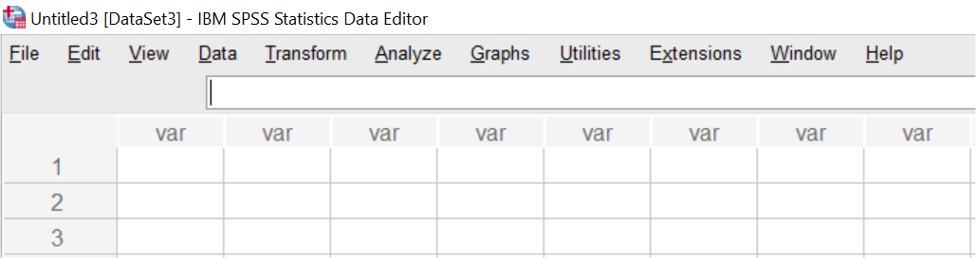
\includegraphics{img/0.1.png}
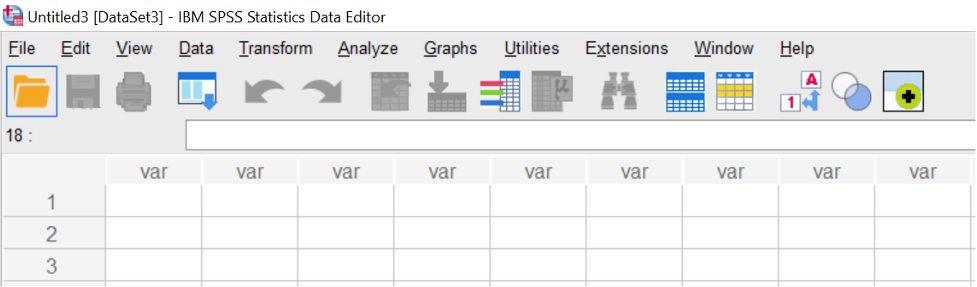
\includegraphics{img/0.2.png}

\#\#\#\#Adjusting the Font Size
The default font size in SPSS files is small for many readers. If you would like to increase the size of the font in the data file, please click View and Fonts to adjust the font for your preferences. Increasing the size of the font in the output file seems a bit more complicated. You can increase the size of the font in the output pane easily by clicking View and Outline Size; however, the font within the main section of the file is not so easily changed. To increase the size of the tables generated, please click Edit and Options and select the Pivot Tables tab. Within the pop-up window (shown below), change from System Default to Large Font (click to highlight this option) and click OK.

\hypertarget{opening-spss-and-the-spss-layout}{%
\subsection{Opening SPSS and the SPSS layout}\label{opening-spss-and-the-spss-layout}}

Your lab instructor will take you through the process of opening the SPSS program. You may double-click on its icon located on the desktop of your lab computer, or you may find it using the Start menu. Once the program loads, you will be prompted with a pop-up window that asks you which file you would like to open. For now, we will be examining the basic layout of SPSS without a data set, so you can click {Cancel}.

Once you do, the main SPSS spreadsheet should open. It will look like this, a basic spreadsheet:

\includegraphics{img/1.4.11.png}
Notice at the bottom of your window there are two tabs; ``Data View'' and ``Variable View''. In data view, we enter data into our spreadsheet. You will notice that rows are numbered on the left-hand side of the spreadsheet, while columns are labeled ``var''. This is an indication of the general structure of SPSS: Variables are contained in the columns, and rows indicate individual observations. For example, if you obtained the heights (in inches) of 5 people \{x= 64, 70, 63, 62, 65\} and wanted to enter their data into SPSS, each person's height would be entered in a new row, not across the columns, as seen below:

\includegraphics{img/1.4.12.png}

\hypertarget{reviewing-variable-properties-and-the-variable-view-tab}{%
\subsubsection{Reviewing variable properties and the Variable View tab}\label{reviewing-variable-properties-and-the-variable-view-tab}}

Now that we have some data entered, we might want to name our variable so that it's evident our measurements represent heights. In order to view or modify variable names and other properties, look to the bottom of your SPSS window and switch over to the ``Data View'' tab. Once you do this, your window will appear as follows:

\includegraphics{img/1.4.13.png}

Here, you can edit the name of your variables, and specify their properties. Variable names can be anything you like, with the restriction that you cannot use numbers or spaces. Next, notice several other important properties of variables you may at some point need to set or modify:

\begin{itemize}
\tightlist
\item
  Name: the name of your variable that will appear as a colum header in Data View. No spaces or numerals.
\item
  Type: Your data will most often be Numeric, but sometimes, as in data representing currency or data in scientific notation, you may change the data type appropriately. If your data is simply a label, word, or response (such as an open-ended response to a survey question), choose ``String'': this tells SPSS not to treat this variable as a number. (Nota bene: if you select the wrong type of variable, SPSS may not be able to process your requested calculations, so always remember to check this parameter!)
\item
  Width: This refers to how many digits will be visible by default.
\item
  Decimals: This refers to how many decimal places will be visible by default.
\item
  Label: This is a description of the variable. Any information too long to be included in the variable name goes here.
\item
  Values: For nominal scale data, let's say 1 represents male and 2 represents female, this is where you include the values and their corresponding labels.
\item
  Measure: This variable property allows you to specify the nature of your data. Depending on the kind of scale you are using, you will choose a different measure type. Nominal and ordinal are chosen for nominal and ordinal scales, respectively. ``Scale'' is used when your data is measured on a ratio or interval scale.
\end{itemize}

\hypertarget{practice-problems}{%
\subsection{Practice Problems}\label{practice-problems}}

\begin{enumerate}
\def\labelenumi{\arabic{enumi}.}
\item
  In your assigned breakout room, collect information to use in a data file. For each member of your group, collect preferred name, year of study (1, 2, 3, etc.), and type of personal device used (Mac, PC, Chromebook, etc.). Remember to check the settings of the variables in Variable View. You should each create an SPSS data file with the collected information, and upload that file in Moodle under the ``SPSS Basics -- Data File Submission'' link.
\item
  A data file has been provided for you in Moodle. Open that file and answer the questions in the Moodle quiz entitled ``Reading an SPSS Data File.''
\end{enumerate}

\hypertarget{jamovi---week-1---january-9th-10th}{%
\section{JAMOVI - Week 1 - January 9th \& 10th}\label{jamovi---week-1---january-9th-10th}}

In our lab sessions, we will be using jamovi to help us with the analyses about which we are learning in classes. Throughout each lab, we will show you how to use jamovi to solve specific problems, and then you will use the examples to solve in-lab assignments, homework, and the analysis for your team project.

\hypertarget{getting-started-with-jamovi}{%
\subsection{Getting Started with jamovi}\label{getting-started-with-jamovi}}

This section, including its associated figures, is copied almost verbatim, with some minor editorial changes, from \href{https://www.learnstatswithjamovi.com/}{Learning statistics with jamovi: A tutorial for psychology students and other beginners, Version 0.70}, according to its \href{https://creativecommons.org/licenses/by-sa/4.0/deed.ast}{CC license}. Thank you to Navarro \& Foxcroft (2019).

In this {[}section{]}, I'll discuss how to get started in jamovi. I'll briefly talk about how to download and install jamovi, but most of the chapter will be focused on getting you started with finding your way around the jamovi GUI. Our goal in this chapter is not to learn any statistical concepts: we're just trying to learn the basics of how jamovi works and get comfortable interacting with the system. To do this, we'll spend a bit of time looking at datasets and variables. In doing so, you'll get a bit of a feel for what it's like to work in jamovi.

However, before going into any of the specifics, it's worth talking a little about why you might want to use jamovi at all. Given that you're reading this, you've probably got your own reasons. However, if those reasons are \emph{because that's what my stats class uses}, it might worth explaining a little why your lecturer has chosen to use jamovi for the class. Of course, I don't really know why \emph{other} people choose jamovi, so I'm really talking about why I use it.

\begin{itemize}
\item
  It's sort of obvious but worth saying anyway: doing your statistics on a computer is faster, easier and more powerful than doing statistics by hand. Computers excel at mindless repetitive tasks, and a lot of statistical calculations are both mindless and repetitive. For most people, the only reason to ever do statistical calculations with pencil and paper is for learning purposes. In my class, I do occasionally suggest doing some calculations that way, but the only real value to it is pedagogical. It does help you to get a ``feel'' for statistics to do some calculations yourself, so it's worth doing it once. But only once!
\item
  Doing statistics in a conventional spreadsheet (e.g., Microsoft Excel) is generally a bad idea in the long run. Although many people likely feel more familiar with them, spreadsheets are very limited in terms of what analyses they allow you do. If you get into the habit of trying to do your real life data analysis using spreadsheets, then you've dug yourself into a very deep hole.
\item
  Avoiding proprietary software is a very good idea. There are a lot of commercial packages out there that you can buy, some of which I like and some of which I don't. They're usually very glossy in their appearance and generally very powerful (much more powerful than spreadsheets). However, they're also very expensive. Usually, the company sells ``student versions'' (crippled versions of the real thing) very cheaply, and then they sell full-powered ``educational versions'' at a price that makes me wince. They will also sell commercial licenses with a staggeringly high price tag. The business model here is to suck you in during your student days and then leave you dependent on their tools when you go out into the real world. It's hard to blame them for trying, but personally I'm not in favour of shelling out thousands of dollars if I can avoid it, and you can avoid it. If you make use of packages like jamovi that are open source and free, you never get trapped having to pay exorbitant licensing fees.
\item
  Something that you might not appreciate now, but will love later on if you do anything involving data analysis, is the fact that jamovi is basically a sophisticated front end for the free R statistical programming language. When you download and install R you get all the basic ``packages'' and those are very powerful on their own. However, because R is so open and so widely used, it's become something of a standard tool in statistics and so lots of people write their own packages that extend the system. And these are freely available too. One of the consequences of this, I've noticed, is that if you look at recent advanced data analysis textbooks then a \emph{lot} of them use R.
\end{itemize}

Those are the main reasons I use jamovi. It's not without its flaws, though. It's relatively new\textsuperscript{1}{[}As of writing this in August 2018.{]} so there is not a huge set of textbooks and other resources to support it, and it has a few annoying quirks that we're all pretty much stuck with, but on the whole I think the strengths outweigh the weakness; more so than any other option I've encountered so far.

\hypertarget{installing-jamovi}{%
\subsubsection{Installing jamovi}\label{installing-jamovi}}

Okay, enough with the sales pitch. Let's get started. Just as with any piece of software, jamovi needs to be installed on a \emph{computer}, which is a magical box that does cool things and delivers free ponies. Or something along those lines; I may be confusing computers with the iPad marketing campaigns. Anyway, jamovi is freely distributed online and you can download it from the jamovi homepage, which is:

\href{https://www.jamovi.org/}{jamovi Homepage}

As previously indicated, the content of this section comes from \href{https://www.learnstatswithjamovi.com/}{Learning statistics with jamovi: A tutorial for psychology students and other beginners, Version 0.70}, according to its \href{https://creativecommons.org/licenses/by-sa/4.0/deed.ast}{CC license}. \textbf{While Navarro \& Foxcroft (2019) discuss an earlier version, you will download the most current version of jamovi that is appropriate for your technology. The most current version will be used in PSYC 292 Labs. If you need help, please refer to any resources posted on your lab Moodle site and/or visit the lab instructor prior to your first lab.}

At the top of the page, under the heading ``Download,'' you'll see separate links for Windows users, Mac users, and Linux users. If you follow the relevant link, you'll see that the online instructions are pretty self-explanatory. As of this writing, the current version of jamovi is 0.9, but they usually issue updates every few months, so you'll probably have a newer version.\textsuperscript{2}{[}Athough jamovi is updated frequently, it doesn't usually make much of a difference for the sort of work we'll do in this book. In fact, during the writing of the book, I upgraded several times, and it didn't make much difference at all to what is in this book.{]}

\hypertarget{starting-jamovi-up}{%
\subsubsection{Starting jamovi up}\label{starting-jamovi-up}}

One way or another, regardless of what operating system you're using, it's time to open jamovi and get started. When first starting jamovi, you will be presented with a user interface which looks something like {[}the figure below{]}.

As previously noted in this section, this figure is copied from \href{https://www.learnstatswithjamovi.com/}{Learning statistics with jamovi: A tutorial for psychology students and other beginners, Version 0.70}, according to its \href{https://creativecommons.org/licenses/by-sa/4.0/deed.ast}{CC license}. Thank you to Navarro \& Foxcroft (2019).

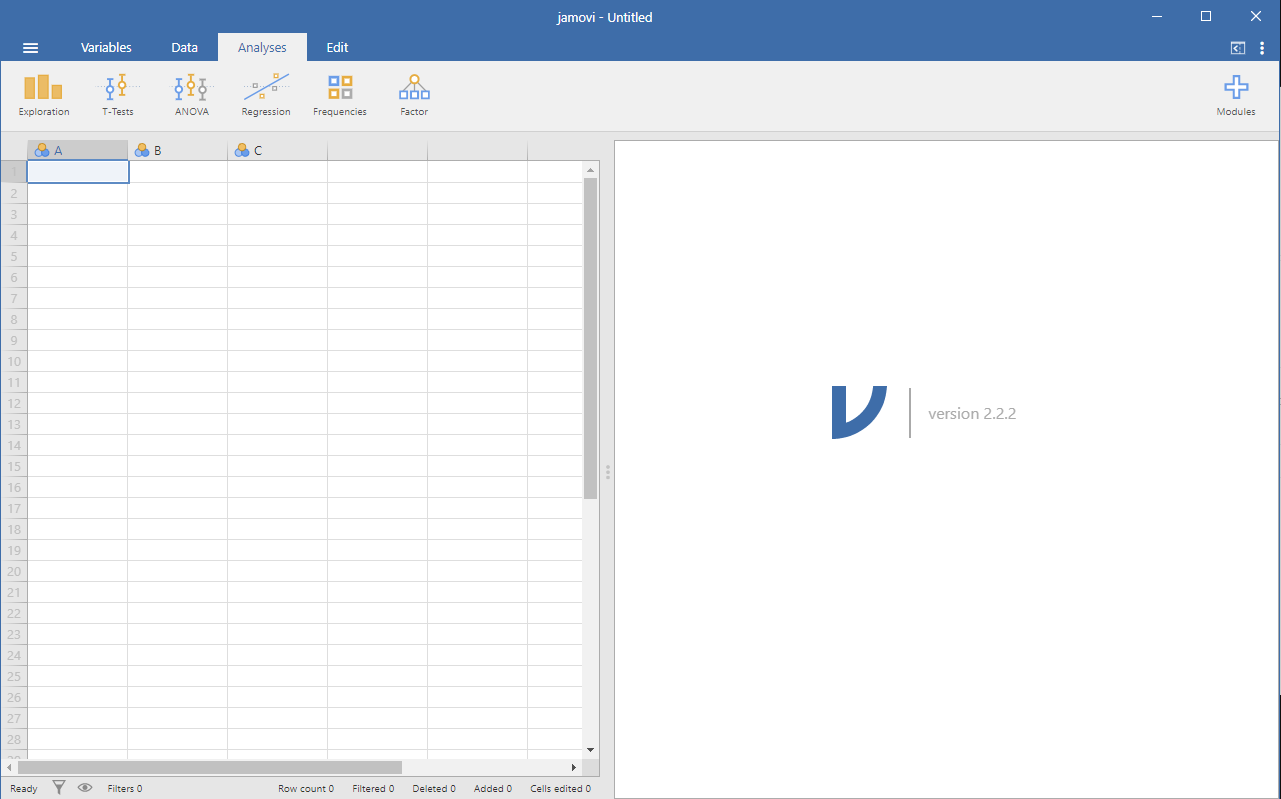
\includegraphics{img/startingjamovi.png}

To the left is the spreadsheet view, and to the right is where the results of statistical tests appear. Down the middle is a bar separating these two regions, and this bar can be dragged to the left or the right to change the sizes of the two view.

It is possible to simply begin typing values into the jamovi spreadsheet as you would in any other spreadsheet software. Alternatively, existing data sets in the CSV (.csv) file format can be opened in jamovi. Additionally, you can easily import SPSS, SAS, Stata and JASP files directly into jamovi. To open a file, select the File tab (three horizontal lines signify this tab) at the top left hand corner, select \texttt{Open} and then choose from the files listed on ``Browse'' depending on whether you want to open an example or a file stored on your computer.

\hypertarget{analyses}{%
\subsection{Analyses}\label{analyses}}

Analyses can be selected from the analysis ribbon or menu along the top. Selecting an analysis will present an \texttt{Options} panel for that particular analysis, allowing you to assign different variables to different parts of the analysis and to select different options. At the same time, the results for the analysis will appear in the right \texttt{Results} panel and will update in real-time as you make changes to the options.

When you have the analysis set up correctly, you can dismiss the analysis options by clicking the arrow to the top right of the optional panel. If you wish to return to these options, you can click on the results that were produced. In this way, you can return to any analysis that you (or say, a colleague) created earlier.

If you decide you no longer need a particular analysis, you can remove it with the results context menu. Right-clicking on the analysis results will bring up a menu, and by selecting \texttt{Analysis} and then \texttt{Remove}, the analysis can be removed. But more on this later. First, let's take a more detailed look at the spreadsheet view.

\hypertarget{the-spreadsheet}{%
\subsection{The Spreadsheet}\label{the-spreadsheet}}

In jamovi, data is represented in a spreadsheet with each column representing a \textbf{\emph{variable}} and each row representing a \textbf{\emph{case}} or \textbf{\emph{participant}}.

\hypertarget{variables}{%
\subsubsection{Variables}\label{variables}}

The most commonly used variables in jamovi are \textbf{Data Variables}, these variables simply contain data either loaded from a data file, or \emph{typed in} by the user. Data variables can be one of three measurement levels:

As previously noted in this section, this figure is copied from \href{https://www.learnstatswithjamovi.com/}{Learning statistics with jamovi: A tutorial for psychology students and other beginners, Version 0.70}, according to its \href{https://creativecommons.org/licenses/by-sa/4.0/deed.ast}{CC license}. Thank you to Navarro \& Foxcroft (2019).

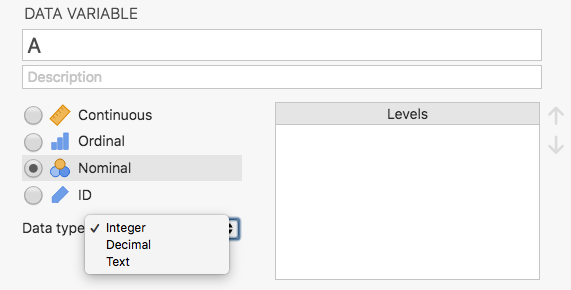
\includegraphics{img/measurementlevels.png}

These levels are designated by the symbol in the header of the variable's column.

The \textbf{\emph{ID}} variable type is unique to jamovi. It's intended for variables that contain identifiers that you would almost never want to analyze, for example, a person's name or a participant ID. Specifying an ID variable type can improve performance when interacting with very large data sets.

\textbf{\emph{Nominal}} variables are for categorical variables which are text labels, for example, a column called Gender with the values Male and Female would be nominal. So would a person's name. Nominal variable values can also have a numeric value. These variables are used most often when importing data which codes values with numbers rather than text. For example, a column in a dataset may contain the values 1 for males and 2 for females. It is possible to add nice, \emph{human-readable} labels to these values with the variable editor (more on this later).

\textbf{\emph{Ordinal}} variables are like Nominal variables, except the values have a specific order. An example is a Likert scale with 3 being \emph{strongly agree} and -3 being \emph{strongly disagree}.

\textbf{\emph{Continuous}} variables are variables which exist on a continuous scale. Examples might be height or weight. Continuous scales are also referred to as \textbf{Interval} or \textbf{Ratio} scale.

In addition, you can also specify different data types: variables have a data type of either \emph{Text}, \emph{Integer}, or \emph{Decimal}.

When starting with a blank spreadsheet and typing values in, the variable type will change automatically depending on the data you enter. This is a good way to get a feel for which variable types go with which sorts of data. Similarly, when opening a data file, jamovi will try to guess the variable type from the data in each column. In both cases, this automatic approach may not be correct, and it may be necessary to manually specify the variable type with the variable editor.

The variable editor can be opened by selecting \texttt{Setup} from the data tab or by double-clicking on the variable column header. The variable editor allows you to change the name of the variable and, for data variables, the variable type, the order of the levels, and the label displayed for each level. Changes can be applied by clicking the \texttt{tick} to the top right. The variable editor can be dismissed by clicking the \texttt{Hide} arrow.

New variables can be inserted or appended to the data set using the \texttt{Add} button from the data ribbon. The \texttt{Add} button also allows the addition of computed variables.

\hypertarget{computed-variables---week-5---february-6th-7th}{%
\subsubsection{Computed Variables - Week 5 - February 6th \& 7th}\label{computed-variables---week-5---february-6th-7th}}

Computed Variables are those which take their value by performing a computation on other variables. Computed Variables can be used for a range of purposes, including log transforms, \emph{z}-scores, sum-scores, negative scoring, and means.

One way computed variables can be added to the data set with the {Add} button available on the {Data} tab. This will produce a drop-down menu in which you select where you want the variable to be placed. If you select {Insert} under the heading ``Computed Variable,'' the new computed variable appears to the left of the currently highlighted variable. If you select {Append}, the variable goes to the far right of all variables currently included (think ``Appendix''). Alternatively, under the {Data} menu tab, you could select {Compute}. This command will lead to the newly computed variable appearing to the right of your currently highlighted variable. After making your selection, a formula box where you can specify the formula will appear. The usual arithmetic operators are available. Some examples of formulas are:

A + B

LOG10(len)

MEAN(A, B)

(dose - VMEAN(dose)) / VSTDEV(dose)

In order, these are the sum of A and B, a log (base 10) transform of len, the mean of A and B, and the \emph{z}-score of the variable dose. The figure below shows the jamovi screen for the new variable computed as the \emph{z}-score of dose (from the `Tooth Growth' example data set).

As previously noted in this section, this figure is copied from \href{https://www.learnstatswithjamovi.com/}{Learning statistics with jamovi: A tutorial for psychology students and other beginners, Version 0.70}, according to its \href{https://creativecommons.org/licenses/by-sa/4.0/deed.ast}{CC license}. Thank you to Navarro \& Foxcroft (2019).

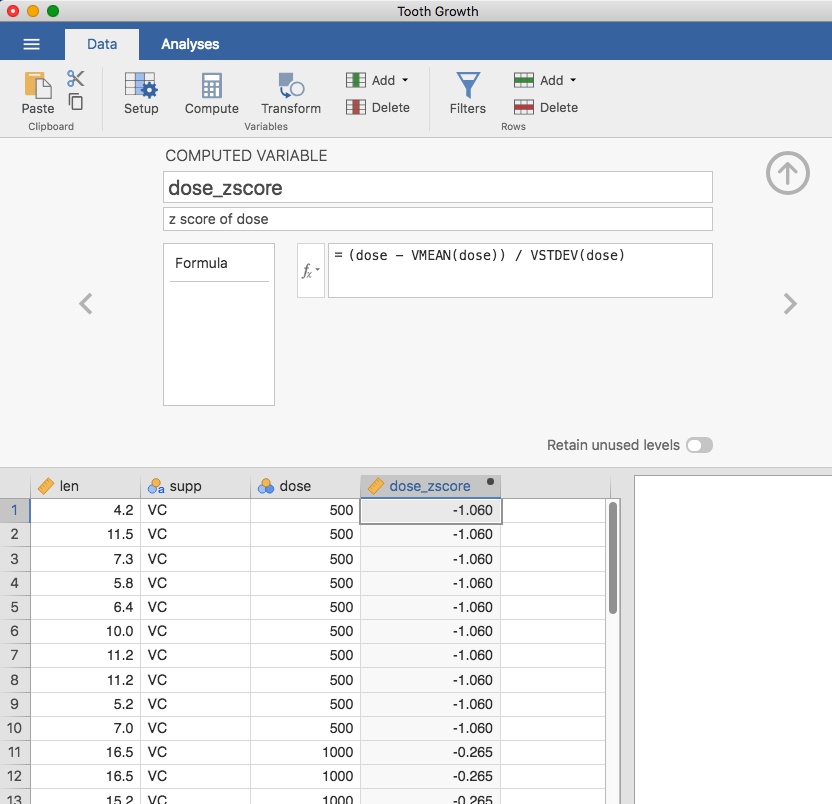
\includegraphics[width=0.75\linewidth]{img/computedvariable}

\caption{A newly computed variable, the z-score of `dose'.}

\emph{V-functions}.\\
Several functions are already available in jamovi and available from the drop down box labelled \emph{f\textsubscript{x}}. A number of functions appear in pairs, one prefixed with a V and the other not. V functions perform their calculation on a variable as a whole whereas non-V functions perform their calculation row by row. For example, MEAN(A, B) will produce the mean of A and B for each row whereas VMEAN(A) gives the mean of all the values in A.

\hypertarget{rationale-for-recoding}{%
\paragraph{Rationale for Recoding}\label{rationale-for-recoding}}

This section and its subsection was developed by Sherry Neville-MacLean. This content is added to what was presented by Navarro \& Foxcroft (2019) for the purposes of a lab lesson.

As you may recall from classes about research methods, one problem researchers using surveys face is response bias on the part of their participants. There are different kinds of response bias. For our purposes, consider participants who tire of answering survey questions and decide to select all extreme responses. These data are not useful.

As one way to catch extreme responses, the researcher can word some of survey questions in the opposite way. Imagine an example where the researcher is using a scale on which ``extremely agree'' indicates participants score high on the construct being measured (ex. gratitude). Consider this survey statement: ``On most days, I feel I have things in my life for which I am grateful.'' A response of ``extremely agree'' indicates gratitude. The researcher may reword some statements in the questionnaire so that ``extremely agree'' indicates the participants score low on the construct. After rewording, another statement on the gratitude questionnaire might read like this: ``I wish I were as fortunate as other people in my life who often come by success and/or material things more easily than I do.'' A response of ``extremely agree'' indicates lack of gratitude.

To be able to look at individual survey respondents' score across all questions, their overall score on the gratitude scale, the researcher often, first, must recode some ``negatively'' worded items' scores. In the above example, the second answer would need to be recoded before being considered with the answer to the first item, the ``positively'' worded statement.

\hypertarget{an-example-of-recoding-and-computing-a-new-variable}{%
\subparagraph{An Example of Recoding and Computing a New Variable}\label{an-example-of-recoding-and-computing-a-new-variable}}

The following demonstration of how to recode data and compute a new variable is done using the example of the Perceived Stress Scale. This measurement tool is from Cohen, S., \& Williamson, G. (1988). Psychological stress in a probability sample of the United States. In S. Spacapan \& S. Oskamp (Eds.), \emph{The social psychology of health: Claremont Symposium on Applied Social Psychology} (pp.~31--67). Newbury Park, CA: Sage. \textbf{This material is being used educational purposes. Please be sure to follow copyright laws if you plan to reuse this material.}

Let's consider a scale that is often used as a measure of stress in psychological studies, the Perceived Stress Scale, by Cohen and Williamson (1988). We can walk through the process of recoding data and data computations with this example. Let's begin by looking at the scale itself.

\textbf{Perceived Stress Scale}

\emph{Instructions}: The questions in this scale ask you about your feelings and thoughts during the last month. In each case, you will be asked to indicate how often you felt or thought a certain way. Although some of the questions are similar, there are differences between them and you should treat each one as a separate question. The best approach is to answer each question fairly quickly. That is, don't try to count up the number of times you felt a particular way, but rather indicate the alternative that seems like a reasonable estimate.

For each question, chose from the following alternatives:

0 = never

1 = almost never

2 = sometimes

3 = fairly often

4 = very often

\emph{Questions}: In the last month, how often have you\ldots{}

\begin{enumerate}
\def\labelenumi{\arabic{enumi}.}
\item
  been upset because of something that happened unexpectedly?
\item
  felt that you were unable to control the important things in your life?
\item
  felt nervous and ``stressed''?
\item
  felt confident about your ability to handle your personal problems?
\item
  felt that things were going your way?
\item
  found that you could not cope with all the things that you had to do?
\item
  been able to control irritations in your life?
\item
  felt that you were on top of things?
\item
  been angered because of things that happened that were outside of your control?
\item
  felt difficulties were piling up so high that you could not overcome them?
\end{enumerate}

Those questions that are negatively worded in terms of the construct will be reverse coded before moving forward to a calculation.

Indicate the numbers of the items that appear to be worded in terms that scoring a 4 (very often) would represent showing stress (the construct). (\emph{Notice: This question is not asking you if the construct of stress is positive or negative. It is asking if answering the question with a 4 would indicate a high level of the construct.}) Write your answers on a sheet or in a document.

Indicate the numbers of the items that appear to be worded in terms that scoring a 4 (very often) would represent showing lack of stress (the construct). (\emph{Notice: This question is not asking you if the construct is positive or negative. It is asking if answering the question with a 4 would indicate lack of the construct.}) Write your answers on the same sheet or in the same document.

Check your answers:
If you answered that scoring a 4 on questions 1, 2, 3, 6, 9, and 10 would indicate stress, you are correct.
If you answered that scoring a 4 on questions 4, 5, 7, and 8 would indicate lack of stress, you are correct!

Notice that the ``Stress'' scale in the PSYC 291 Survey data dictionary is adapted from the PSS. In the PSYC 291 Survey, respondents were asked about these items, but for the past week, not the past month. The levels of the response options were the same as the PSS. For some reason, however, the data in the data set range from 1 to 5. It seems reasonable that 1 represents ``never'' and 5 represents ``very often,'' and we will proceed using this idea of the scale anchors.

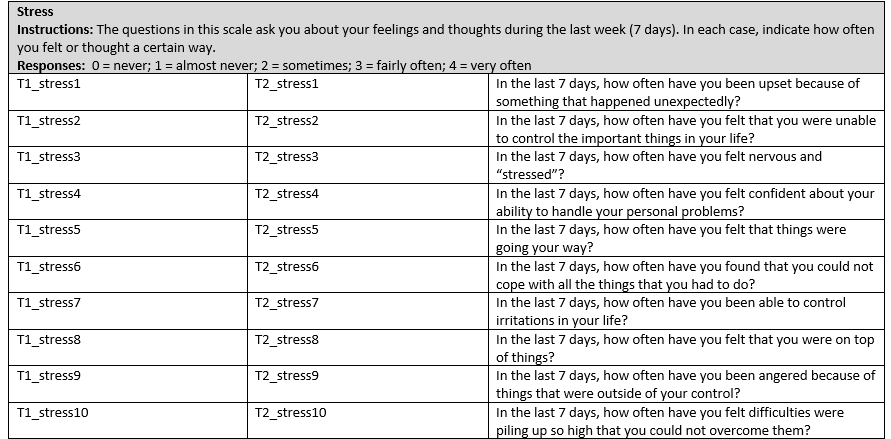
\includegraphics{img/StressScaleFromPSYC291Survey.png}

Let's work through the process of computing a new variable (a composite variable) using the Stress items for T1 in the PSYC 291 Survey data file. As you can see in the data dictionary, T1 is ``during the first week of classes in September.'' The first step to computing the new variable is recoding. We need to recode items 4, 5, 7, and 8 before we can compute a composite score for all Stress items.

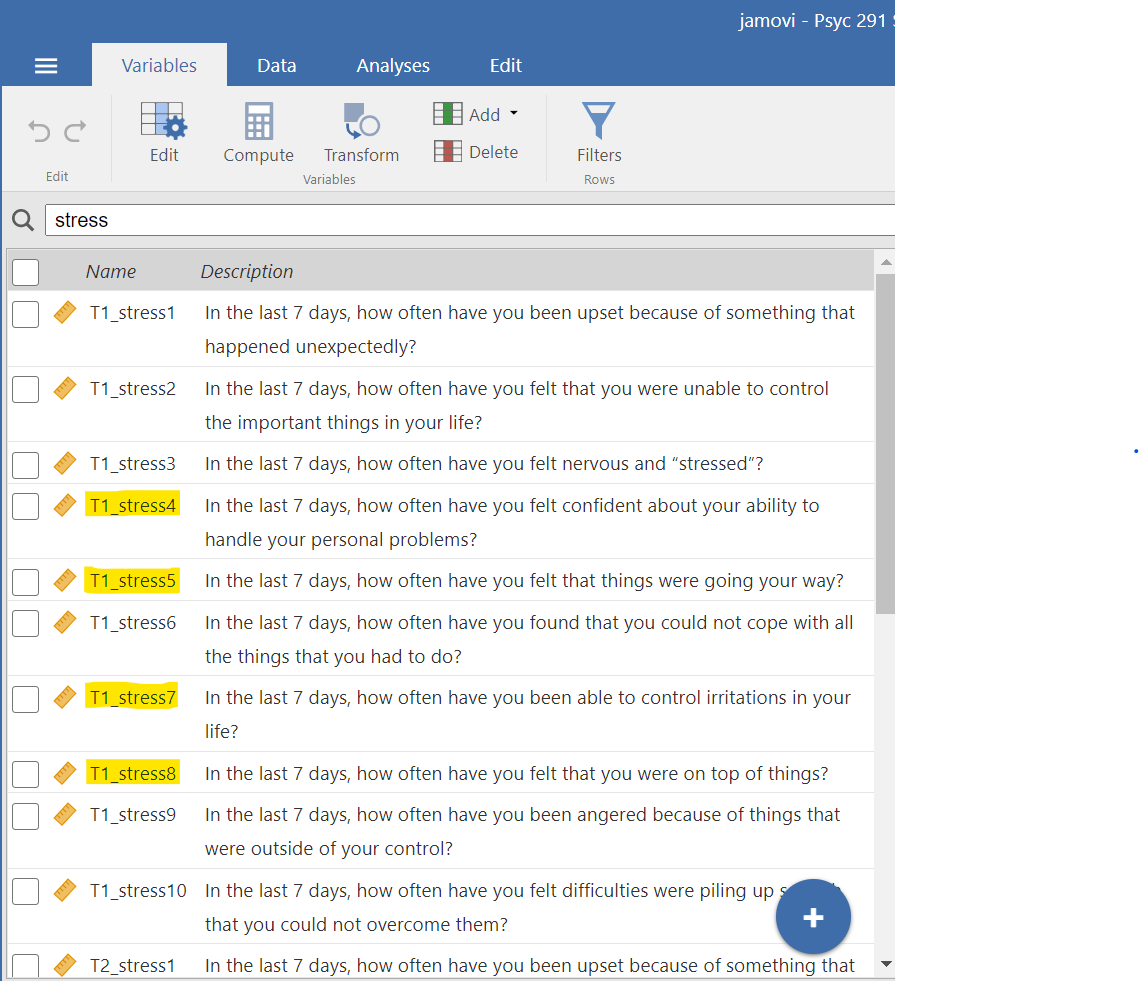
\includegraphics{img/StressScale_ShowingVariablesToRecode.png}

We will begin by recoding item 4, shown as \texttt{T1\_stress4} in the data file. While the column for that item is highlighted, select {Data}, and then, select {Transform}.

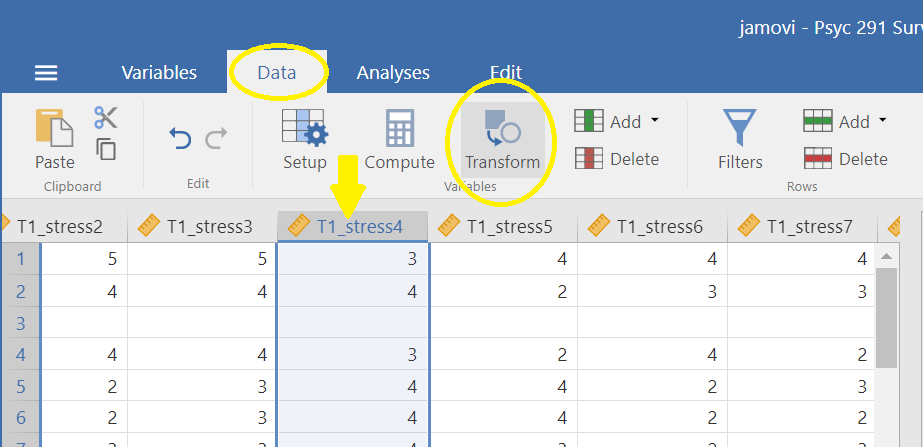
\includegraphics{img/StressScale_CommandsToRecode.png}

A new column will appear to the right of the column for the \texttt{T1\_stress4} and the variable attributes panel will drop down. (As you can imagine, you could also use these commands: {Data}, {Add}, and under ``Transformed Variable,'' either {Insert} or {Append}.) You can fill in the information for what you want this variable to be called and record its notable attributes. For our purposes, let's call it \texttt{T1\_stress4\_Recoded}. You can see that the source variable is correctly shown as \texttt{T1\_stress4}.

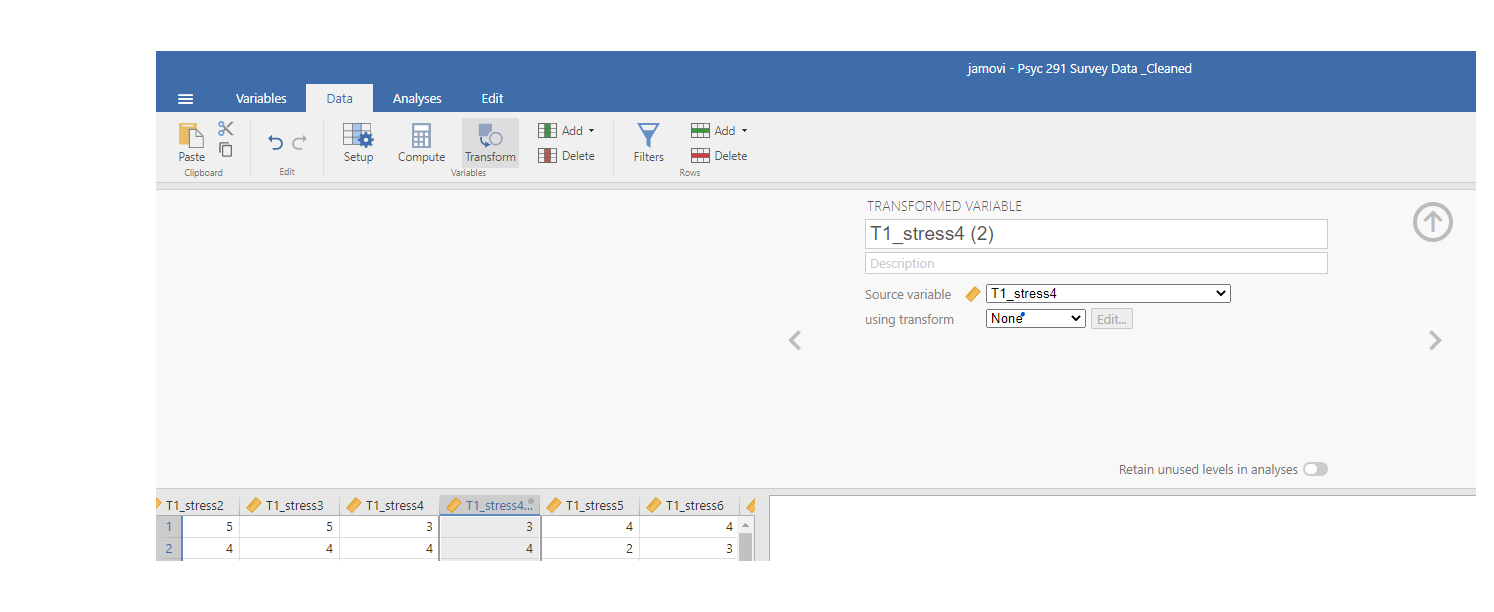
\includegraphics{img/StressScale_CommandsToRecodeT1Stress4.png}

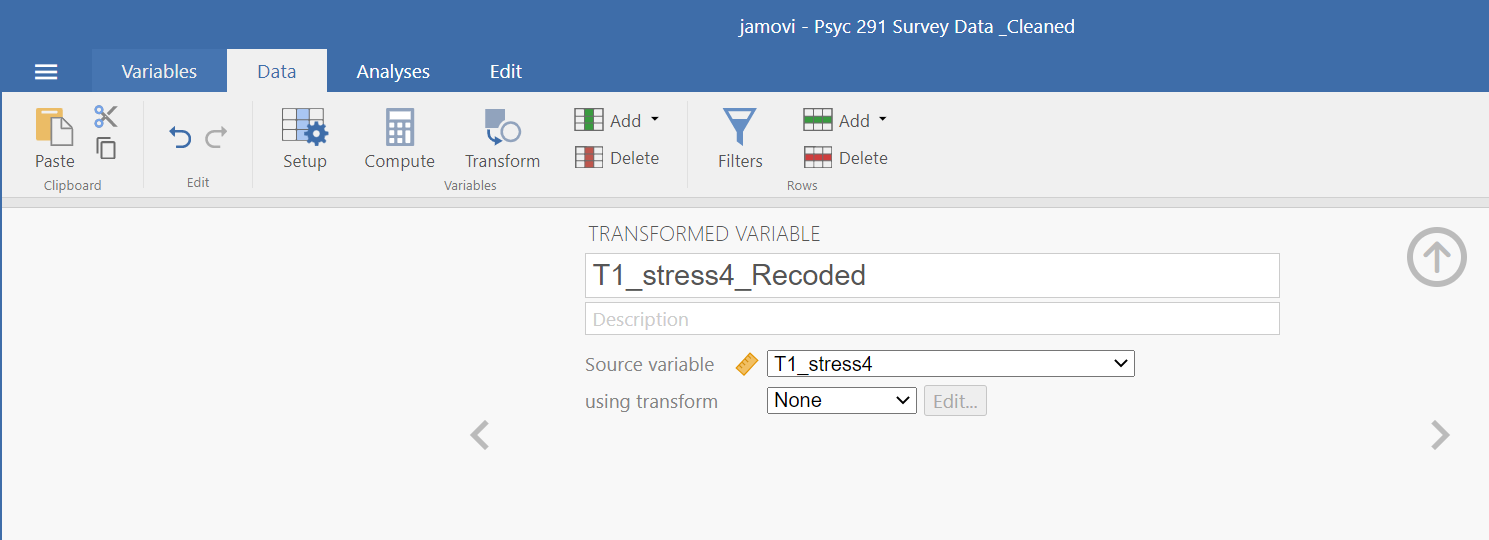
\includegraphics{img/StressScale_RenamingT1Stress4RecodedVariable.png}

Now, it is time to add the transform rule that you want used. Click on the white box after ``using transform'' and select {Create New Transform}.

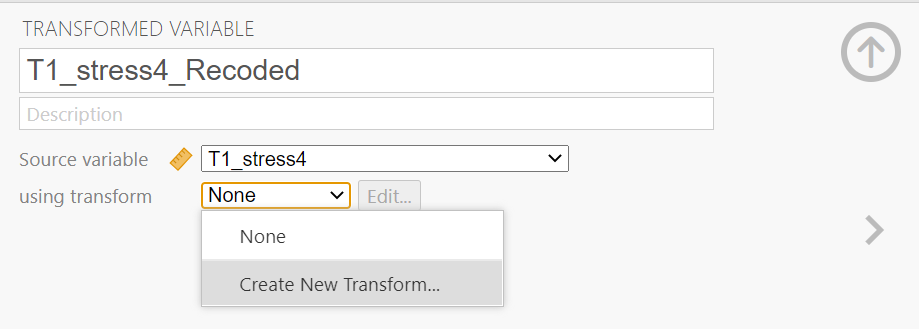
\includegraphics{img/StressScale_TransformationToRecodeT1Stress4.png}

When you do click that button, a new panel will appear.

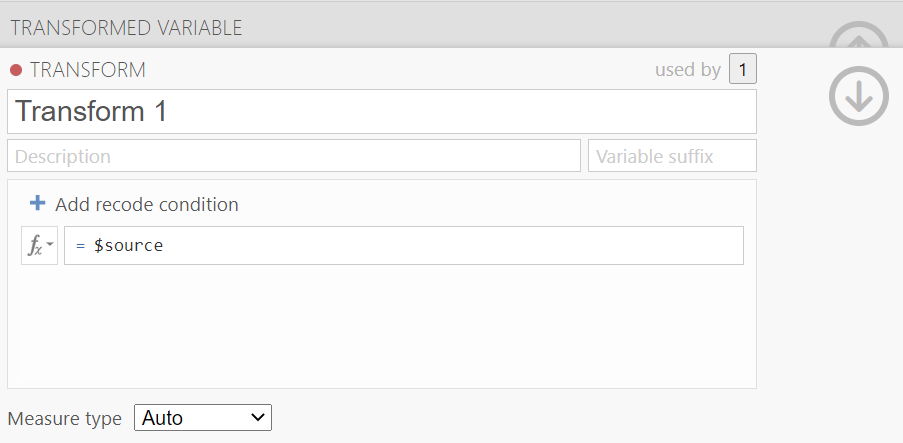
\includegraphics{img/StressScale_TransformationToRecodeT1Stress4_2.png}

Let's fill in the information to tell JAMOVI what we want done to the data. We will give the transformation a name (``Reverse\_Coding'') and click the {Show formula editor} button which looks like \emph{f\textsubscript{x}}.

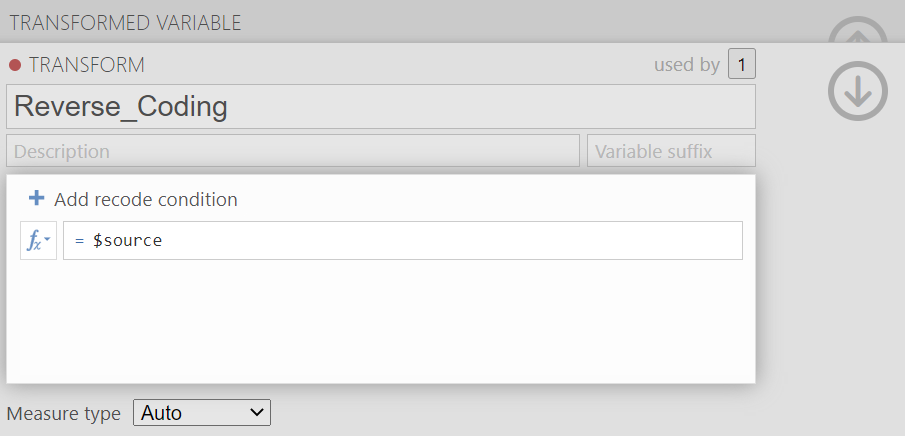
\includegraphics{img/StressScale_TransformationToRecodeT1Stress4_3.png}

A new panel opens, and we will enter the formula to have the transformations calculated.

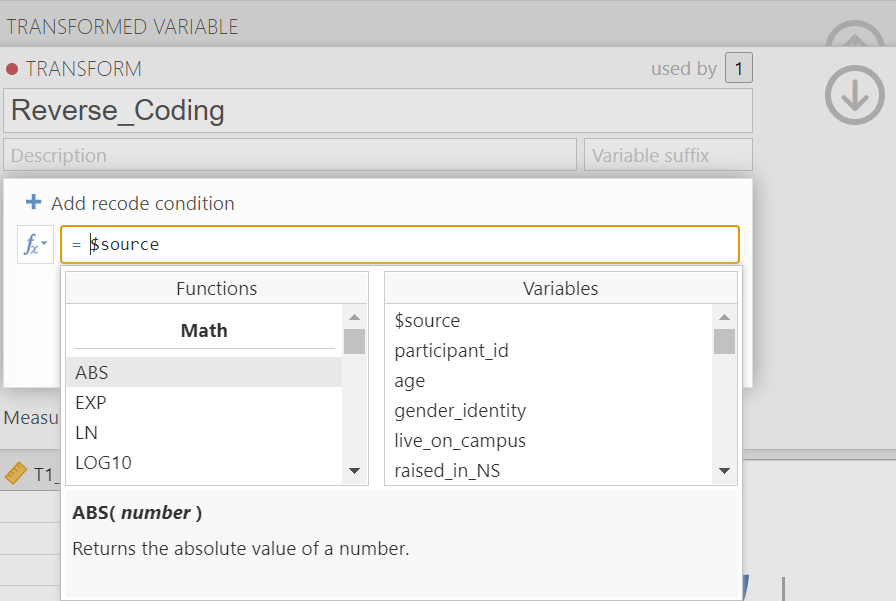
\includegraphics{img/StressScale_TransformationToRecodeT1Stress4_4.png}

Because 5 is the maximum score value and 1 is the minimum score value, we can write this equation to get the recoded values:

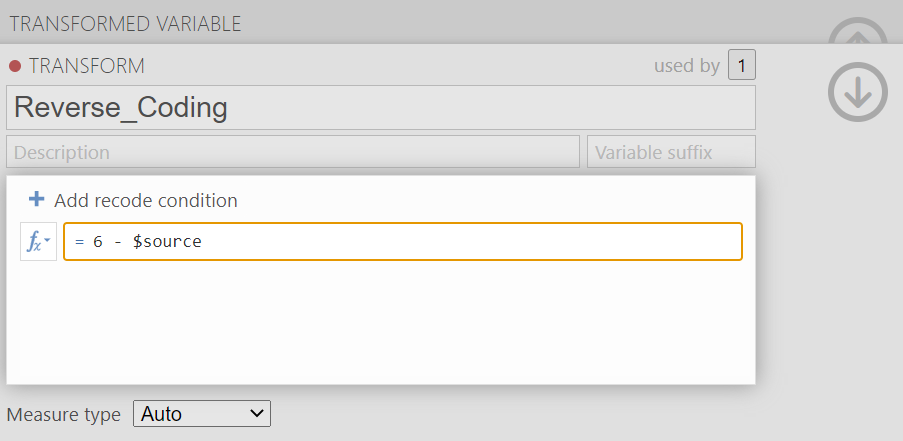
\includegraphics{img/StressScale_TransformationToRecodeT1Stress4_5.png}

Go ahead and check the math on each of those recoded values!

To close the transformation panel, click on the downward facing arrow.

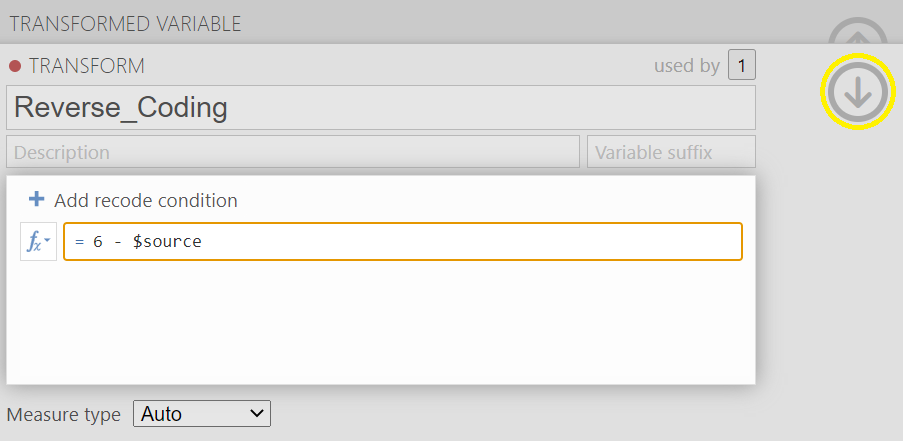
\includegraphics{img/StressScale_TransformationToRecodeT1Stress4_6.png}

To get out of the Transformed Variable panel, click on the upward facing arrow.

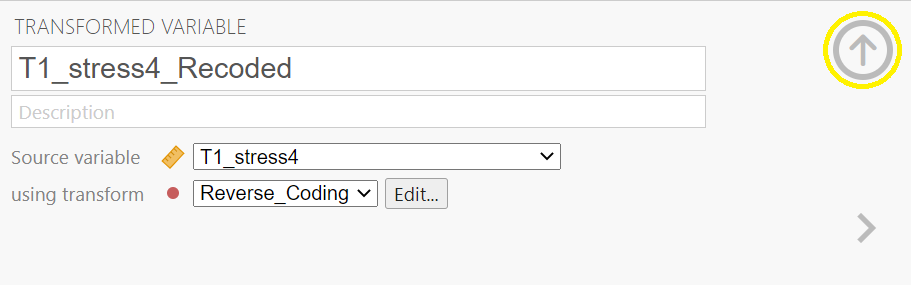
\includegraphics{img/StressScale_TransformationToRecodeT1Stress4_7.png}

You should see the recoded T1\_stress4 value in the \texttt{T1\_stress4\_Recoded} column.

Repeat the steps to recode \texttt{T1\_stress5}, \texttt{T1\_stress7}, and \texttt{T1\_stress8}. For these cases, you will not need to select {Create New Transform}. Instead, you will select the transformation rule you already created, {Reverse\_Coding }.

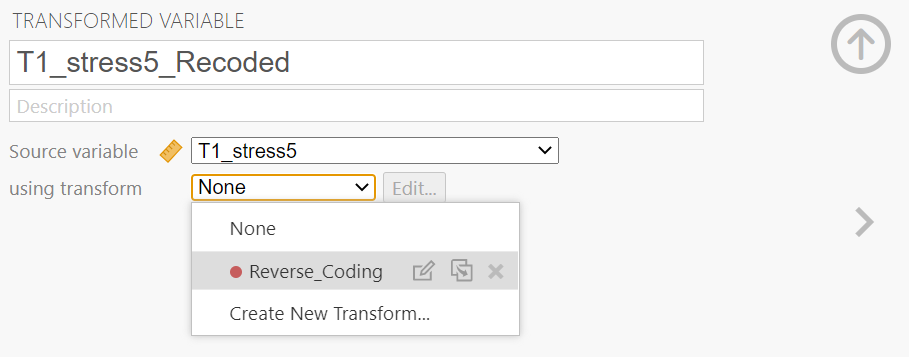
\includegraphics{img/StressScale_TransformationToRecodeT1Stress4_8.png}

Now, you can see all 4 recoded values. Notice the transformed variables are noted with red circles by their names at the top of the columns.

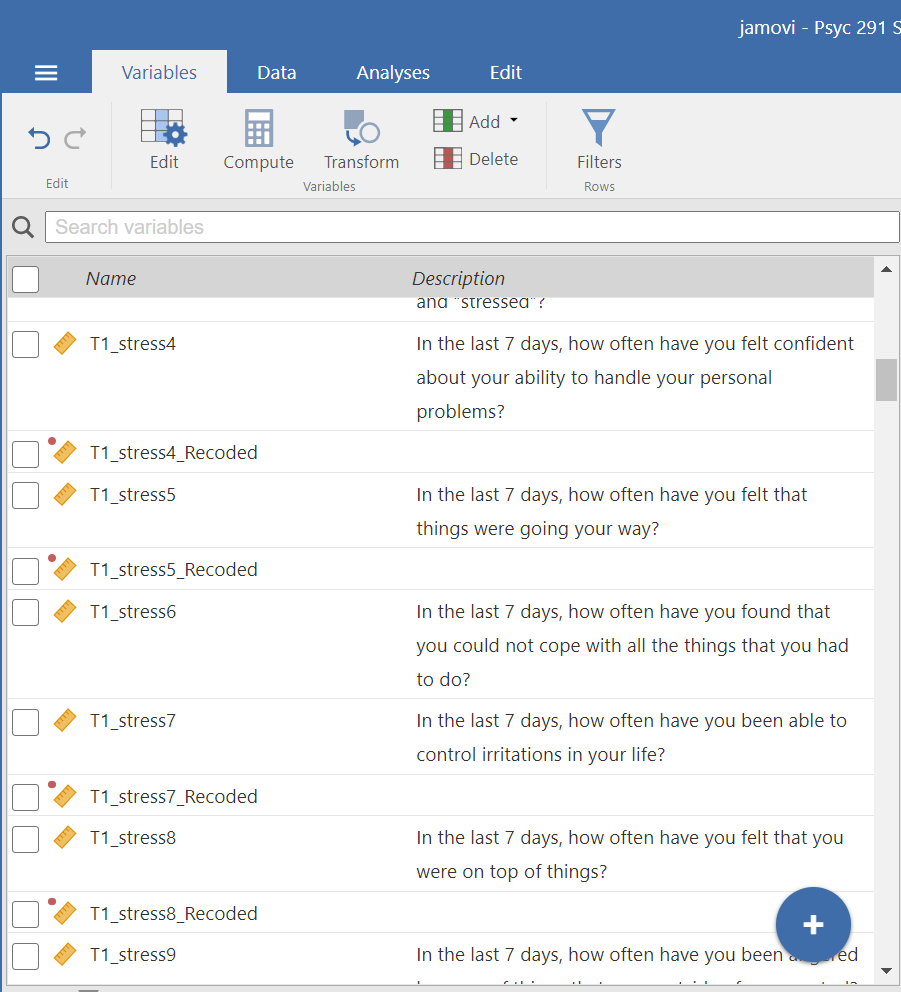
\includegraphics{img/StressScale_TransformationToRecodeT1Stress4_9.png}

Recall the scoring instructions say that after recoding the values for these scale items, we should sum the scores. Let's do that now.
Move to the column for \texttt{T1\_stress10}, highlight that column, and select {Data} and select {Compute}.

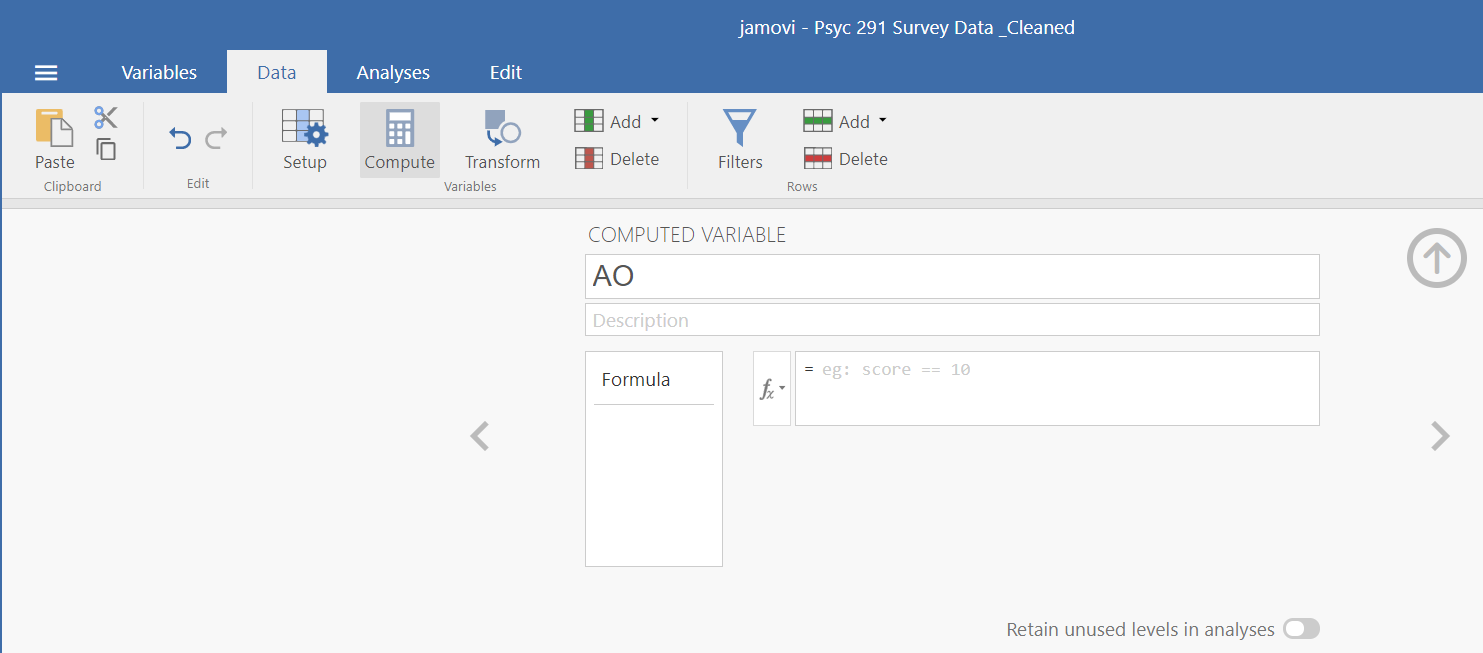
\includegraphics{img/StressScale_ComputationCommands.png}

If the Computed Variable panel does not drop down for you, click on {Setup} while the column for the new variable is highlighted.

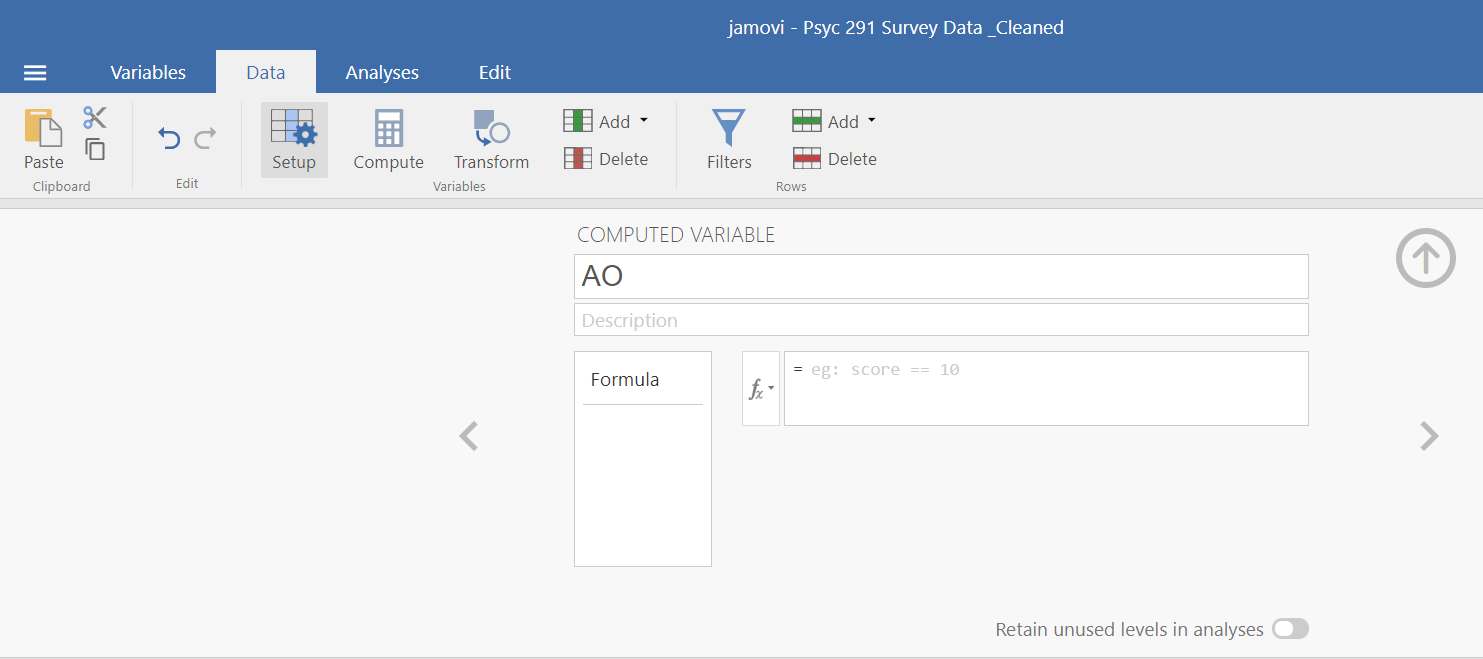
\includegraphics{img/StressScale_ComputationCommands_2.png}

Let's fill in the variable attributes and enter the formula for JAMOVI to follow to compute the sum. Remember, we want to include the recoded values for items 4, 5, 7, and 8. We do not want to include the original values for those items. One way to calculate the sum is by using the SUM command in the formula editor and placing all variable names you want included in the sum in the brackets behind the word SUM with commas between the variable names. Alternatively, you could select each variable name and use plus signs between them.

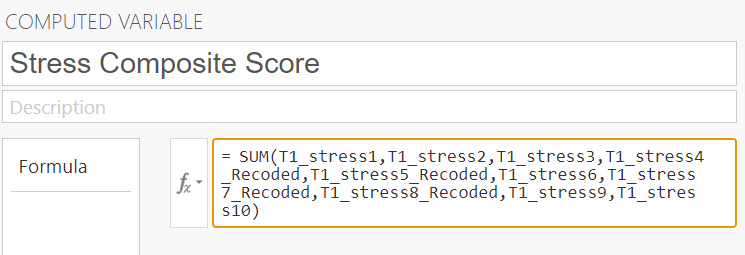
\includegraphics{img/StressScale_ComputationFormula1.png}

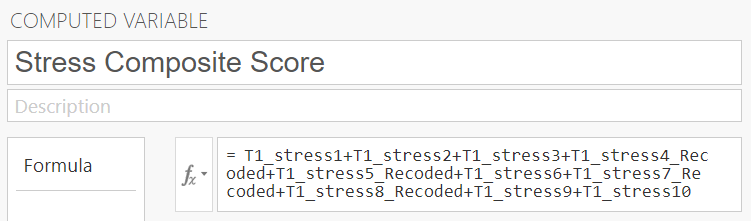
\includegraphics{img/StressScale_ComputationFormula2.png}

As you did with the Transformed Variable panel, you can close the Computed Variable panel by clicking the upward facing arrow.
This may seem like a lot of work to do for a score on one variable; however, you can imagine these commands and having JAMOVI do this recoding and computation work is a mega timesaver when you are working with a large data set or recoding and/or computations of many variables.

\hypertarget{z-scores-as-a-type-of-computed-variable-in-jamovi}{%
\paragraph{Z-scores (as a Type of Computed Variable in JAMOVI)}\label{z-scores-as-a-type-of-computed-variable-in-jamovi}}

This section was developed by Sherry Neville-MacLean. This content is added to what was presented by Navarro \& Foxcroft (2019) for the purposes of a lab lesson.

There will be times when you want to compute \emph{z}-scores. (For example, you may want to look at a large data set and decide whether you have extreme outliers.) Getting \emph{z}-scores in JAMOVI is very easy.

Let's look at the process to get the \emph{z}-scores for those \texttt{Stress\ Composite\ Score} values.

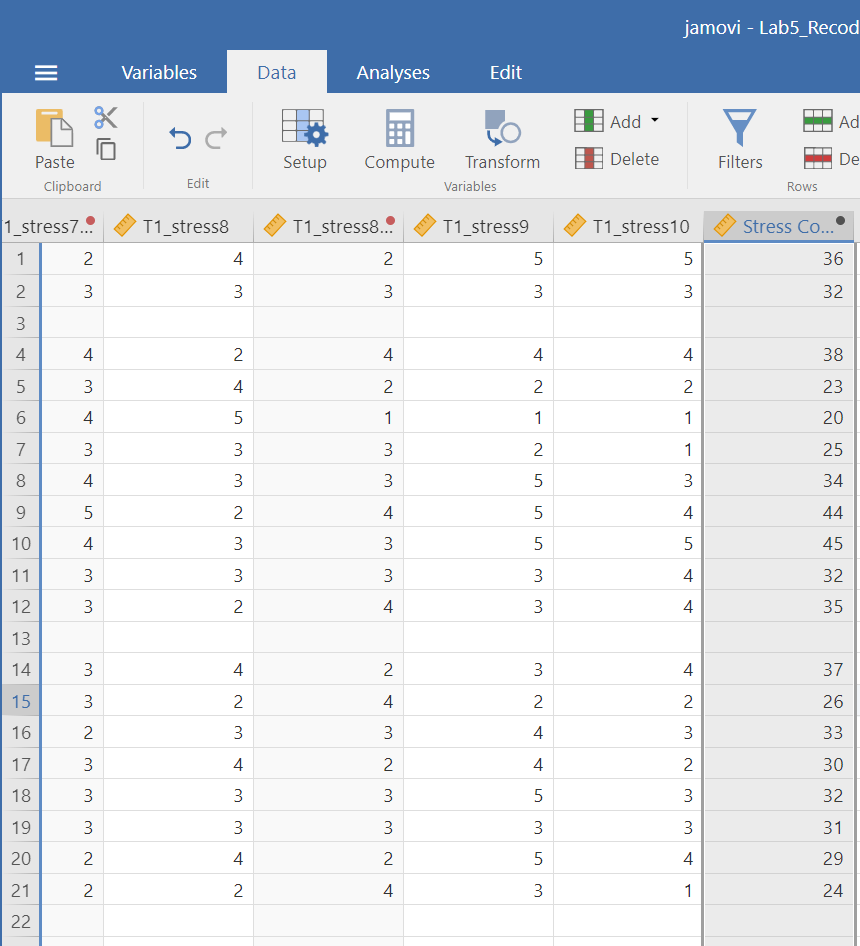
\includegraphics{img/StressScale_Column.png}

In JAMOVI, \emph{z}-scores can be obtained by selecting {Data} and {Compute} after the variable column is highlighted. As before, you can click on {Setup} while the column for the new variable is highlighted to fill in the Computed Variable attributes. When entering those attributes, you should also enter the formula for the \emph{z}-score. The Z is found in the formula editor's drop-down menu, but it can also be typed in. The variable name is in that drop-down menu, too. Similarly, it can be type instead.

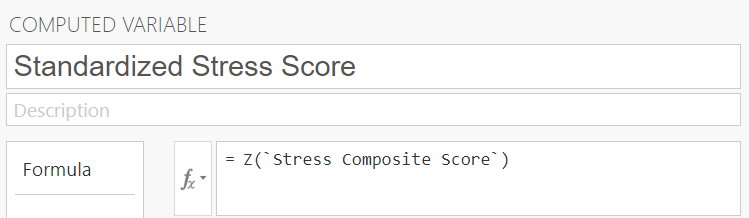
\includegraphics{img/StressScale_ZScoreFormula.png}

Remember to click the upward facing arrow to close the Computed Variable panel. \texttt{Standardized\ Stress\ Score} in the image below depicts the \emph{z}-scores for \texttt{Stress\ Composite\ Score}. Notice that computed variables have a black circle to the right of their name near the top of the column.

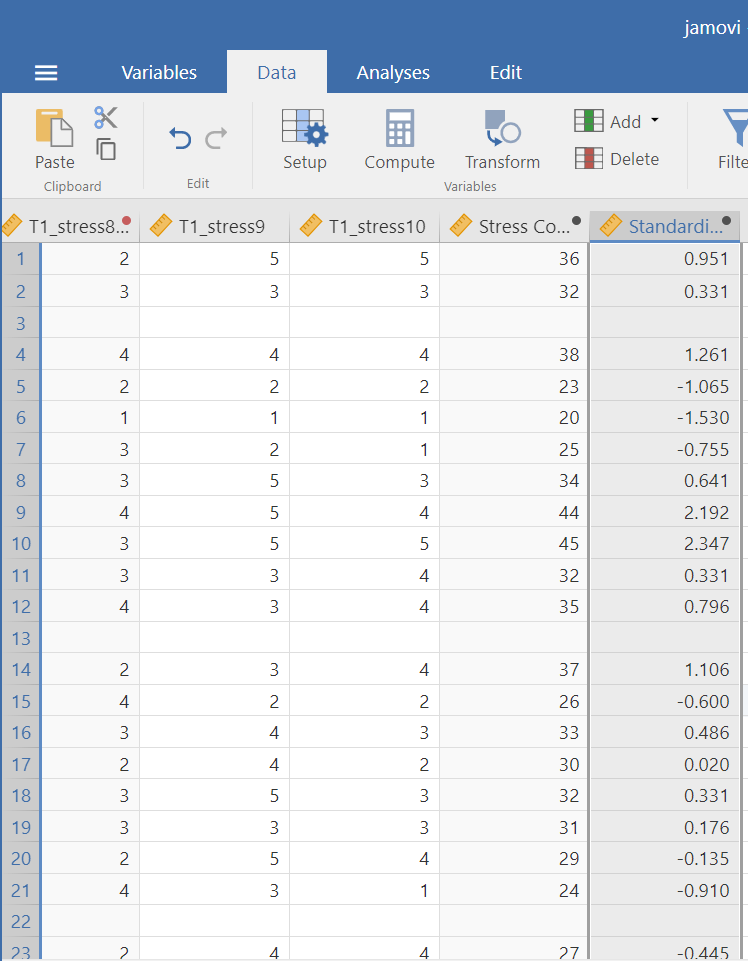
\includegraphics{img/StressScale_ZScoreColumn.png}

\hypertarget{homework}{%
\paragraph{Homework}\label{homework}}

See \href{https://moodle.stfx.ca/course/view.php?id=29319}{Moodle} for homework questions.

\hypertarget{copy-and-paste}{%
\paragraph{Copy and Paste}\label{copy-and-paste}}

jamovi produces nice American Psychological Association (APA) formatted tables and attractive plots. It is often useful to be able to copy and paste these, perhaps into a Word document, or into an email to a colleague. To copy results, right click on the object of interest, and from the menu, select exactly what you want to copy. The menu allows you to choose to copy only the image or the entire analysis. Selecting \texttt{copy} copies the content to the clipboard, and this content can be pasted into other programs in the usual way. You can practice this later on when we do some analyses.

\hypertarget{syntax-mode}{%
\paragraph{Syntax Mode}\label{syntax-mode}}

jamovi also provides an ``R Syntax Mode''. In this mode, jamovi produces equivalent R code for each analysis. To change to syntax mode, select the Application menu to the top right of jamovi (a button with three vertical dots) and click the ``Syntax mode'' checkbox there. You can turn off syntax mode by clicking this a second time.

In syntax mode, analyses continue to operate as before, but now they produce R syntax and \emph{ascii output} like an R session. Like all results objects in jamovi, you can right click on these items (including the R syntax) and copy and paste them, for example into an R session. At present, the provided R syntax does not include the data import step and so this must be performed manually in R. There are many resources explaining how to import data into R and if you are interested we recommend you take a look at these; just search on the interweb.

\hypertarget{loading-data-in-jamovi}{%
\subsection{Loading Data in jamovi}\label{loading-data-in-jamovi}}

There are several different types of files that are likely to be relevant to us when doing data analysis. There are two in particular that are especially important from the perspective of this book:

\begin{itemize}
\item
  \textbf{\emph{jamovi files}} are those with an .omv file extension. This is the standard kind of file that jamovi uses to store data, variables, and analyses.
\item
  \textbf{\emph{Comma separated value (.csv) files}} are those with a .csv file extension. These are just regular old text files and they can be opened with many different software programs. It's quite typical for people to store data in .csv files, precisely because they're so simple.
\end{itemize}

There are also several other kinds of data file that you might want to import into jamovi. For instance, you might want to open Microsoft Excel spreadsheets (.xls files), or data files that have been saved in the native file formats for other statistics software, such as SPSS or SAS. Whichever file formats you are using, it's a good idea to create a folder or folders especially for your jamovi data sets and analyses and to make sure you keep these backed up regularly.

\hypertarget{importing-data-from-csv-files}{%
\subsubsection{Importing Data from CSV Files}\label{importing-data-from-csv-files}}

One quite commonly used data format is the humble \emph{comma separated value} file, also called a .csv file, and usually bearing the file extension .csv. {[}These{]} .csv files are just plain old-fashioned text files, and what they store is basically just a table of data. This is illustrated in {[}the figure below{]}, which shows a file called \filename{booksales.csv} that I've created. As you can see, each row represents the book sales data for one month. The first row doesn't contain actual data though; it has the names of the variables.

As previously noted in this section, this figure is copied from \href{https://www.learnstatswithjamovi.com/}{Learning statistics with jamovi: A tutorial for psychology students and other beginners, Version 0.70}, according to its \href{https://creativecommons.org/licenses/by-sa/4.0/deed.ast}{CC license}. Thank you to Navarro \& Foxcroft (2019).

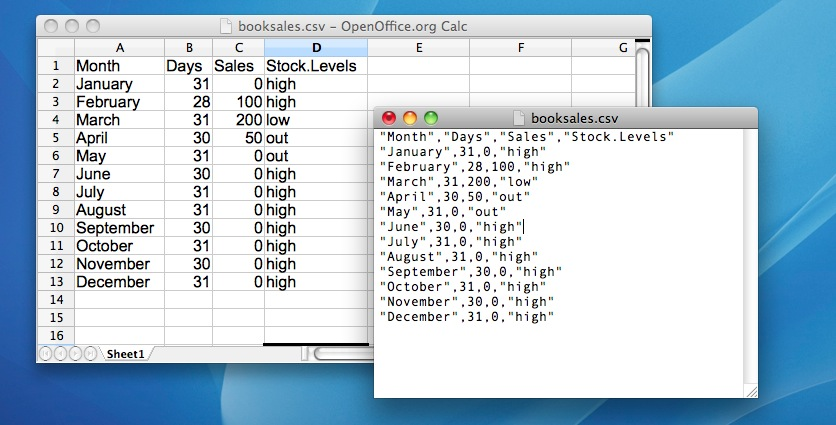
\includegraphics[width=0.75\linewidth]{img/booksalescsv}

\caption{The \filename{booksales.csv} data file. On the left, I've opened the file using a spreadsheet program (OpenOffice), which shows that the file is basically a table. On the right, the same file is open in a standard text editor (the TextEdit program on a Mac), which shows how the file is formatted. The entries in the table are wrapped in quote marks and separated by commas.}

It's easy to open .csv files in jamovi. From the top left menu (the button with three parallel lines), choose \texttt{Open} and browse to where you have stored the csv file on your computer. If you're on a Mac, it'll look like the usual Finder window that you use to choose a file; on Windows, it looks like an Explorer window. An example of what it looks like on a Mac is shown in {[}the following figure{]}. I'm assuming that you're familiar with your own computer, so you should have no problem finding the .csv file that you want to import! Find the one you want, and then click on the ``Open'' button.

As previously noted in this section, this figure is copied from \href{https://www.learnstatswithjamovi.com/}{Learning statistics with jamovi: A tutorial for psychology students and other beginners, Version 0.70}, according to its \href{https://creativecommons.org/licenses/by-sa/4.0/deed.ast}{CC license}. Thank you to Navarro \& Foxcroft (2019).

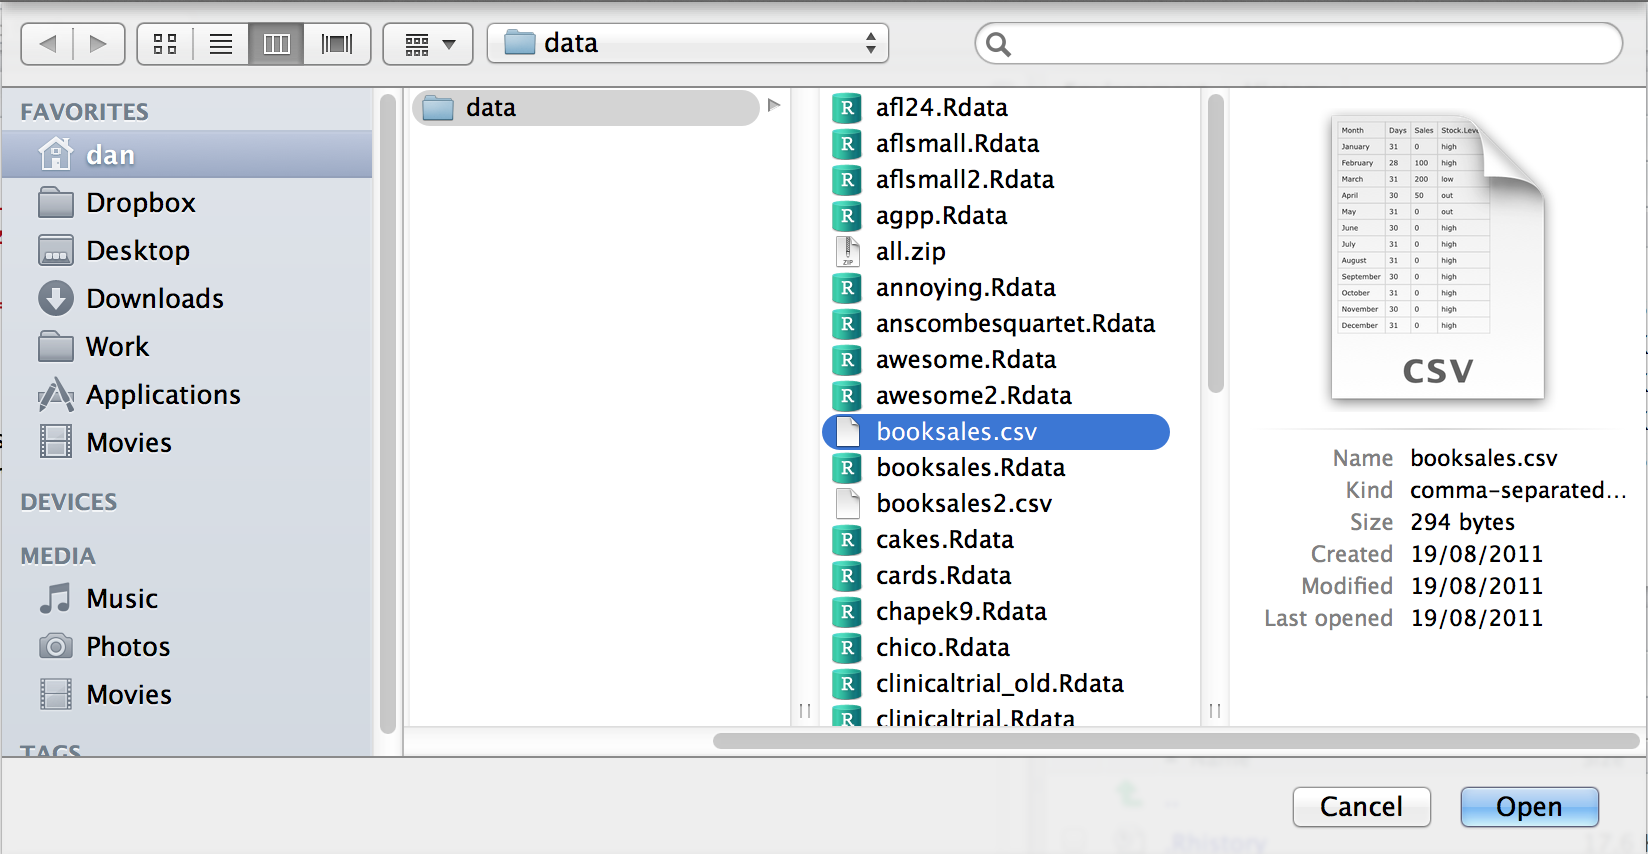
\includegraphics[width=0.75\linewidth]{img/openscreen}

\caption{A dialog box on a Mac asking you to select the .csv file jamovi should try to import. Mac users will recognize this immediately; it's the usual way in which a Mac asks you to find a file. Windows users won't see this; instead, they'll see the usual Explorer window that Windows always gives you when it wants you to select a file.}

There are a few things that you can check to make sure that the data gets imported correctly:

\begin{itemize}
\item
  Heading. Does the first row of the file contain the names for each variable - a \texttt{header} row? The \{booksales.csv\} file has a header, so that's a yes.
\item
  Separator. What character is used to separate different entries? In most .csv files, this will be a comma (it is ``comma separated'' after all).
\item
  Decimal. What character is used to specify the decimal point? In English-speaking countries, this is almost always a period (i.e., \{.\}). That's not universally true though. Many European countries use a comma.
\item
  Quote. What character is used to denote a block of text? That's usually going to be a double quote mark (\{``\}). It is for the \{booksales.csv\} file.
\end{itemize}

\hypertarget{importing-unusual-data-files}{%
\subsection{Importing Unusual Data Files}\label{importing-unusual-data-files}}

Throughout this book, I've assumed that your data are stored as a jamovi \{.omv\} file or as a ``properly'' formatted .csv file. However, in real life, that's not a terribly plausible assumption to make so I'd better talk about some of the other possibilities that you might run into.

\hypertarget{loading-data-from-text-files}{%
\subsubsection{Loading Data from Text Files}\label{loading-data-from-text-files}}

The first thing I should point out is that if your data are saved as a text file but aren't \emph{quite} in the proper .csv format, then there's still a pretty good chance that jamovi will be able to open it. You just need to try it and see if it works. Sometimes, though, you will need to change some of the formatting. The ones that I've often found myself needing to change are:

\begin{itemize}
\item
  \emph{header}. A lot of the time when you're storing data as a .csv file, the first row actually contains the column names and not data. If that's not true, then it's a good idea to open up the .csv file in a spreadsheet programme such as Open Office and add the header row manually.
\item
  \emph{sep}. As the name ``comma separated value'' indicates, the values in a row of a .csv file are usually separated by commas. This isn't universal, however. In Europe, the decimal point is typically written as \{,\} instead of \{.\}, and as a consequence, it would be somewhat awkward to use \{,\} as the separator. Therefore, it is not unusual to use \{;\} instead of \{,\} as the separator. At other times, I've seen a TAB character used.
\item
  \emph{quote}. It's conventional in .csv files to include a quoting character for textual data. As you can see by looking at the \{booksales.csv\} file, this is usually a double quote character, \{``\}. But sometimes there is no quoting character at all, or you might see a single quote mark (') used instead.
\item
  \emph{skip}. It's actually very common to receive .csv files in which the first few rows have nothing to do with the actual data. Instead, they provide a human readable summary of where the data came from, or maybe they include some technical info that doesn't relate to the data.
\item
  \emph{missing values}. Often, you'll be given data with missing values. For one reason or another, some entries in the table are missing. The data file needs to include a ``special'' value to indicate that the entry is missing. By default, jamovi assumes that this value is \{99\}\textsuperscript{3}{[}You can change the default value for missing values in jamovi from the top right menu (three vertical dots), but this only works at the time of importing data files into jamovi. The default missing value in the dataset should not be a valid number associated with any of the variables, e.g.~you could use \{-9999\} as this is unlikely to be a valid value.{]}, for both numeric and text data, so you should make sure that, where necessary, all missing values in the .csv file are replaced with \{99\} (or \{-9999\}; whichever you choose) before opening / importing the file into jamovi. Once you have opened / imported the file into jamovi, all the missing values are converted to blank cells in the jamovi spreadsheet view.
\end{itemize}

\hypertarget{loading-data-from-spss-and-other-statistics-packages}{%
\paragraph{Loading Data from SPSS (and other statistics packages)}\label{loading-data-from-spss-and-other-statistics-packages}}

The commands listed above are the main ones we'll need for data files in this book. But, in real life, we have many more possibilities. For example, you might want to read data files from other statistics programs. Since SPSS is probably the most widely used statistics package in psychology, it's worth mentioning that jamovi can also import SPSS data files (.sav file extension). Just follow the instructions above for how to open a .csv file, but this time navigate to the .sav file you want to import. For SPSS files, jamovi will regard all values as missing if they are regarded as ``system missing'' files in SPSS. The \texttt{Default\ missing} value does not seem to work as expected when importing SPSS files, so be aware of this - you might need another step: import the SPSS file into jamovi, and then export as a .csv file before re-opening in jamovi.\textsuperscript{4}{[}I know this is a bot of a fudge, but it does work, and hopefully this will be fixed in a later version of jamovi.{]}.

And that's pretty much it, at least as far as SPSS goes. As far as other statistical software goes, jamovi can also directly open / import SAS and STATA files.

\hypertarget{loading-excel-files}{%
\paragraph{Loading Excel Files}\label{loading-excel-files}}

A different problem is posed by Excel files. Despite years of yelling at people for sending data to me encoded in a proprietary data format, I get sent a lot of Excel files. The way to handle Excel files is to open them up first in Excel or another spreadsheet programme that can handle Excel files, and then export the data as a .csv file before opening / importing the csv file into jamovi.

\hypertarget{changing-data-from-one-level-to-another}{%
\subsection{Changing Data from One Level to Another}\label{changing-data-from-one-level-to-another}}

Sometimes you want to change the variable level. This can happen for all sorts of reasons. Sometimes when you import data from files, it can come to you in the wrong format. Numbers sometimes get imported as nominal, text values. Dates may get imported as text. Participant ID values can sometimes be read as continuous. Nominal values can sometimes be read as ordinal or even continuous. There's a good chance that sometimes you'll want to convert a variable from one measurement level into another one. Or, to use the correct term, you want to \emph{coerce} the variable from one class into another.

In Section 0.6.3, we saw how to specify different variable levels, and if you want to change a variable's measurement level, then you can do this in the jamovi data view for that variable. Just click the check box for the measurement level you want - continuous, ordinal, or nominal.

\hypertarget{installing-add-on-modules-into-jamovi}{%
\subsection{Installing Add-on Modules into jamovi}\label{installing-add-on-modules-into-jamovi}}

A really great feature of jamovi is the ability to install add-on modules from the jamovi library. These add-on modules have been developed by the jamovi community, i.e., jamovi users and developers who have created special software add-ons that do other, usually more advanced, analyses that go beyond the capabilities of the base jamovi program.

To install add-on modules, just click on the large \large\{``+''\} in the top right of the jamovi window, select \texttt{jamovi-library} and then browse through the various add-on modules that are available. Choose the one(s) you want, and then install them, as in {[}the following figure{]}. It's that easy. The newly installed modules can then be accessed from the \texttt{Analyses} button bar. Try it\ldots useful add-on modules to install include \texttt{scatr} (added under \texttt{Descriptives}) and \texttt{\textbackslash{}R\textbackslash{}\ j}.

As previously noted in this section, this figure is copied from \href{https://www.learnstatswithjamovi.com/}{Learning statistics with jamovi: A tutorial for psychology students and other beginners, Version 0.70}, according to its \href{https://creativecommons.org/licenses/by-sa/4.0/deed.ast}{CC license}. Thank you to Navarro \& Foxcroft (2019).

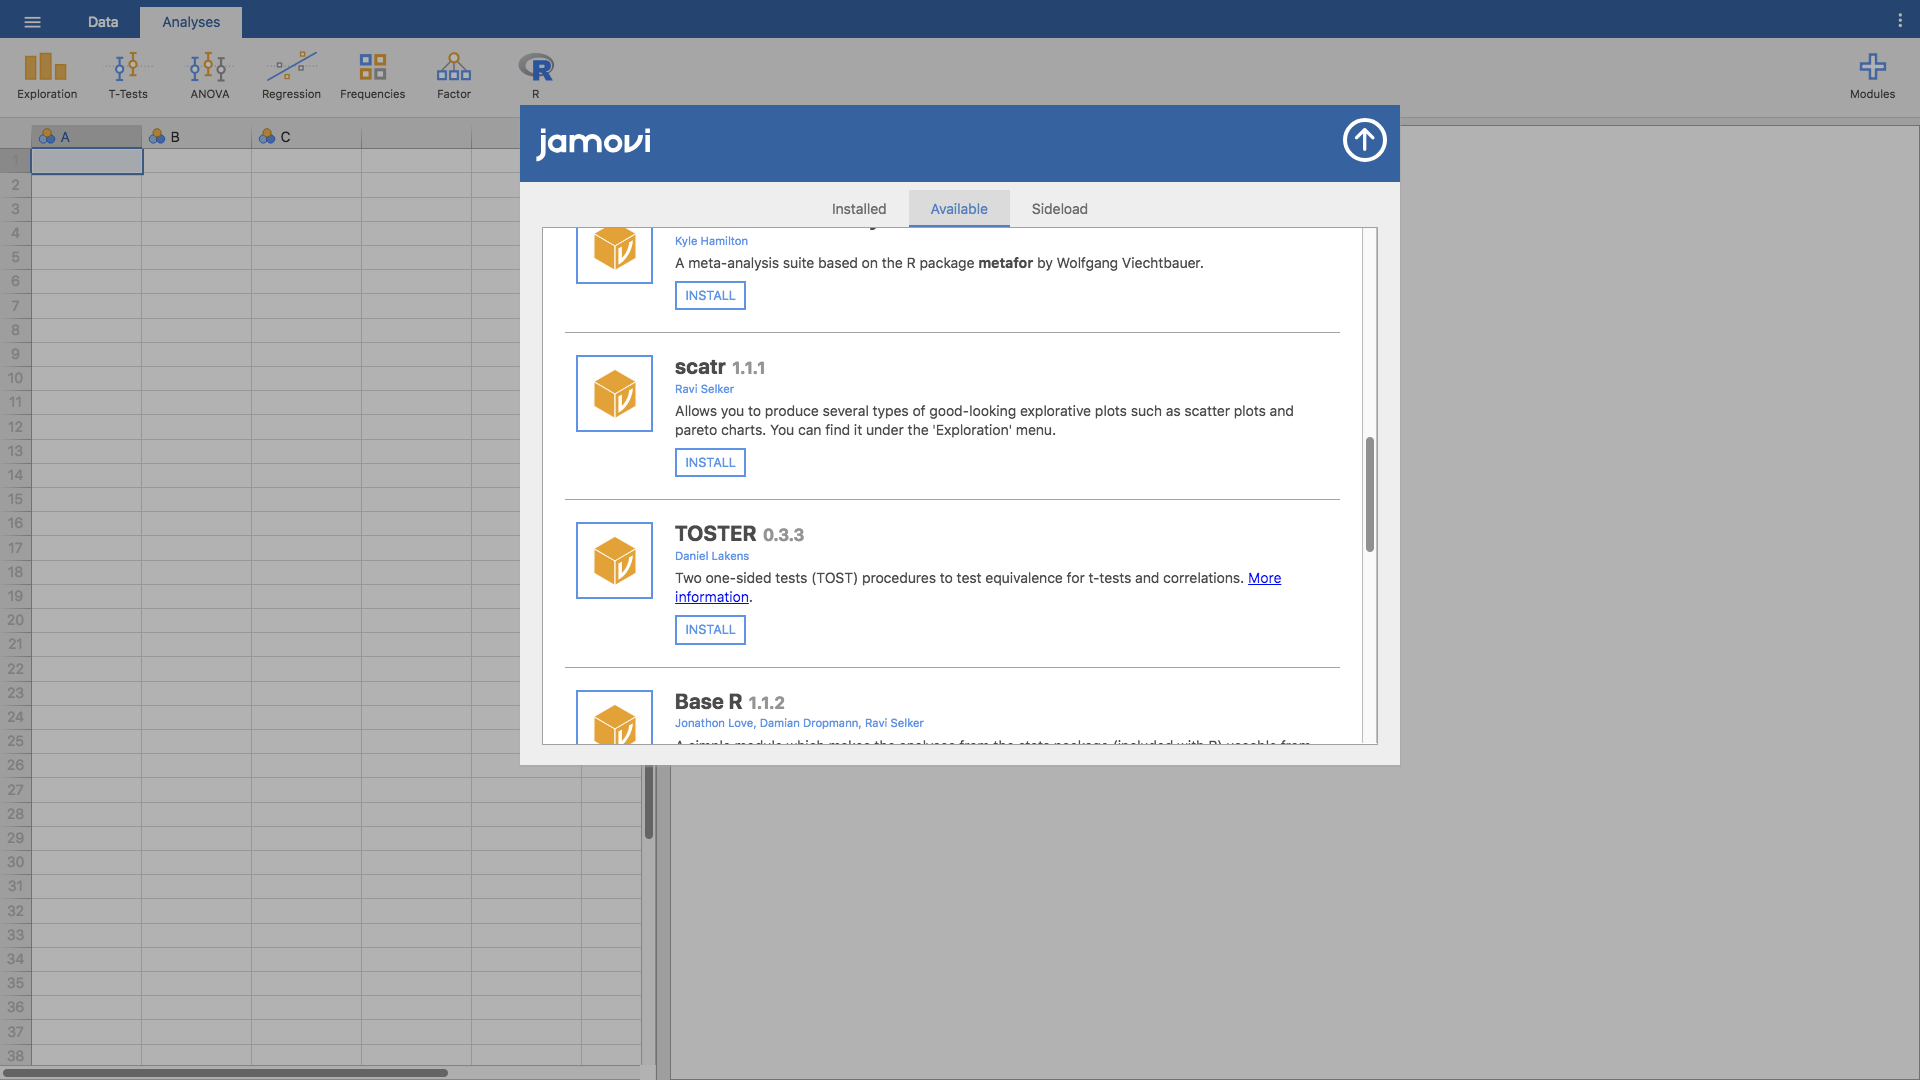
\includegraphics[width=0.75\linewidth]{img/modules}

\caption{Installing add-on modules in jamovi}

\hypertarget{quitting-jamovi}{%
\subsection{Quitting jamovi}\label{quitting-jamovi}}

There's one last thing I should cover in this chapter: how to quit jamovi. It's not hard, just close the program the same way you would any other program. However, what you might want to do before you quit is save your work! There are two parts to this: saving any changes to the data set, and saving the analyses that you ran.

It is good practice to save any changes to the data set as a \emph{new} data set. That way you can always go back to the original data. To save any changes in jamovi, select \texttt{Export...Data} from the main jamovi menu (button with three horizontal bars in the top left) and create a new file name for the changed data set.

Alternatively, you can save \emph{both} the changed data and any analyses you have undertaken by saving as a jamovi file. To do this, from the main jamovi menu select \texttt{Save\ as} and type in a file name for this \texttt{jamovi\ file\ (.omv)}. Remember to save the file in a location where you can find it again later. I usually create a new folder for specific data sets and analyses.

\hypertarget{summary}{%
\subsection{Summary}\label{summary}}

Every book that tries to teach a new statistical software program to novices has to cover roughly the same topics, and in roughly the same order. Ours is no exception, and so in the grand tradition of doing it just the same way everyone else did it, this chapter covered the following topics:

\begin{itemize}
\tightlist
\item
  In Section 0.6.1, we downloaded and installed jamovi, and started it up.
\item
  In Section 0.6.2, we very briefly oriented to the part of jamovi where analyses are done and results appear, but then deferred this until later in the book.
\item
  In Section 0.6.3, we spent more time looking at the spreadsheet part of jamovi, and considered different variable types, and how to compute new variables.
\item
  In Section 0.6.4, we also saw how to load data files in jamovi.
\item
  Then, in Section 0.6.5, we figured out how to open other data files, from different file types.
\item
  In Section 0.6.6, we saw that sometimes we need to coerce data from one type to another.
\item
  According to Section 0.6.7, installing add-on modules from the jamovi community really extends jamovi capabilities.
\item
  Finally, in Section 0.6.8, we looked at good practice in terms of saving your data set and analyses when you have finished and are about to quit jamovi.
\end{itemize}

\noindent
We still haven't arrived at anything that resembles data analysis. Maybe the next Chapter will get us a bit closer!

\hypertarget{lab-1-graphing-data}{%
\chapter{Lab 1: Graphing Data}\label{lab-1-graphing-data}}

{
The commonality between science and art is in trying to see profoundly - to develop strategies of seeing and showing.
-Edward Tufte
}

As we have found out from the textbook and lecture, when we measure things, we get lots of numbers. Too many. Sometimes so many your head explodes just thinking about them. One of \textbf{the most helpful things} you can do to begin to make sense of these numbers, is to look at them in graphical form. Unfortunately, for sight-impaired individuals, graphical summary of data is much more well-developed than other forms of summarizing data for our human senses. Some researchers are developing auditory versions of visual graphs, a process called \textbf{sonification}, but we aren't prepared to demonstrate that here. Instead, we will make charts, and plots, and things to look at, rather than the numbers themselves, mainly because these are tools that are easiest to get our hands on, they are the most developed, and they work really well for visual summary. If time permits, at some point I would like to come back here and do the same things with sonification. I think that would be really, really cool!

\hypertarget{general-goals}{%
\section{General Goals}\label{general-goals}}

Our general goals for this first lab are to get your feet wet, so to speak. We'll do these things:

\begin{enumerate}
\def\labelenumi{\arabic{enumi}.}
\tightlist
\item
  Load in some data to a statistical software program
\item
  Talk a little bit about how the data is structured
\item
  Make graphs of the data so we can look at it and make sense of it.
\end{enumerate}

We will use the EngageNS data to accomplish these goals.

\hypertarget{important-info}{%
\subsection{Important info}\label{important-info}}

\begin{enumerate}
\def\labelenumi{\arabic{enumi}.}
\item
  Data for NYC film permits was obtained from the NYC open data website. The .csv file can be found here: Film\_Permits.csv
\item
  Gapminder data from the gapminder project (copied from the R gapminder library) can be downloaded in .csv format here: gapminder.csv
\end{enumerate}

\hypertarget{r-1}{%
\section{R}\label{r-1}}

\hypertarget{download-the-lab-templates}{%
\subsection{Download the lab templates}\label{download-the-lab-templates}}

You will be completing each lab by writing your code and notes in an R Markdown document.

\begin{enumerate}
\def\labelenumi{\arabic{enumi}.}
\tightlist
\item
  Download the \href{https://github.com/CrumpLab/statisticsLab/raw/master/RMarkdownsLab.zip}{RMarkdownsLab.zip} to your computer.
\item
  Unzip the file, this will produce a new folder with three important parts

  \begin{enumerate}
  \def\labelenumii{\alph{enumii}.}
  \tightlist
  \item
    data folder (contains data files for all labs)
  \item
    LabTemplates folder (contains blank templates for completing all the labs)
  \item
    RMarkdownsLab.Rproj A file with a little blue cube with an R in it.
  \end{enumerate}
\item
  Double-click the RMarkdownsLab.Rproj file, this will automatically open R-studio (if you are at home, you must \href{https://crumplab.github.io/statisticsLab/software.html\#installing-r-and-r-studio}{install R and R-studio first}, or you can use \href{https://crumplab.github.io/statisticsLab/software.html\#r-studio-cloud}{R-studio Cloud} through your web-browser)
\item
  Copy the template .Rmd file for lab 1 from the LabTemplates folder into the main folder, then open it, and use it to begin adding your code and notes for lab 1.
\item
  Watch this screencast to help you get started.
\end{enumerate}

Your lab instructor will show you how to open R-studio on the lab computer. Just find it and double-click. Now you have R-studio. Your lab instructor will also walk you through the steps to get started completing the first lab. We also wrote down the steps \href{https://crumplab.github.io/statisticsLab/software.html\#how-to-complete-the-r-labs}{here}.

There are numerous resources for learning about R, we put some of them on the course website, under the \href{https://crumplab.github.io/psyc3400/Resources.html}{resouces page}. You will find these resources helpful as you learn. We also have a kind of \href{https://crumplab.github.io/statisticsLab/software.html\#r}{general introduction to R and Rstudio here}. This shows you how to download R and R-studio at home (it's free). Throughout the labs you will be writing things called R Markdown documents. You will learn how to do this throughout the labs, but it can also be worthwhile reading other tutorials, such as the one provided by \href{https://rmarkdown.rstudio.com/lesson-1.html}{R Markdown}.

When we made this course, we assumed that most students would be unfamiliar with R and R-studio, and might even be frightened of it, because it is a computer programming language (OOOOHHH NOOOOOOO, I NEED TO DROP THIS COURSE NOW)\ldots Don't worry. It's going to be way easier than you think. Let's compare to other statistics courses where you would learn something like SPSS. That is also a limited programming language, but you would mostly learn how to point with a mouse, and click with button. I bet you already know how to do that. I bet you also already know how to copy and paste text, and press enter. That's mostly what we'll be doing to learn R. We will be doing statistics by typing commands, rather than by clicking buttons. However, lucky for you, all of the commands are already written for you. You just have to copy/paste them.

We know that this will seem challenging at first. But, we think that with lots of working examples, you will get the hang of it, and by the end of the course you will be able to do things you might never have dreamed you can do. It's really a fantastic skill to learn, even if you aren't planning on going on to do research in Psychology (in which case, this kind of thing is necessary skill to learn). With that, let's begin.

\hypertarget{get-some-data}{%
\subsection{Get some data}\label{get-some-data}}

In order to graph data, we need to have some data first\ldots Actually, with R, that's not quite true. Run this bit of code and see what happens:

\begin{Shaded}
\begin{Highlighting}[]
\FunctionTok{hist}\NormalTok{(}\FunctionTok{rnorm}\NormalTok{(}\DecValTok{100}\NormalTok{, }\AttributeTok{mean=}\DecValTok{50}\NormalTok{, }\AttributeTok{sd=}\DecValTok{25}\NormalTok{))}
\end{Highlighting}
\end{Shaded}

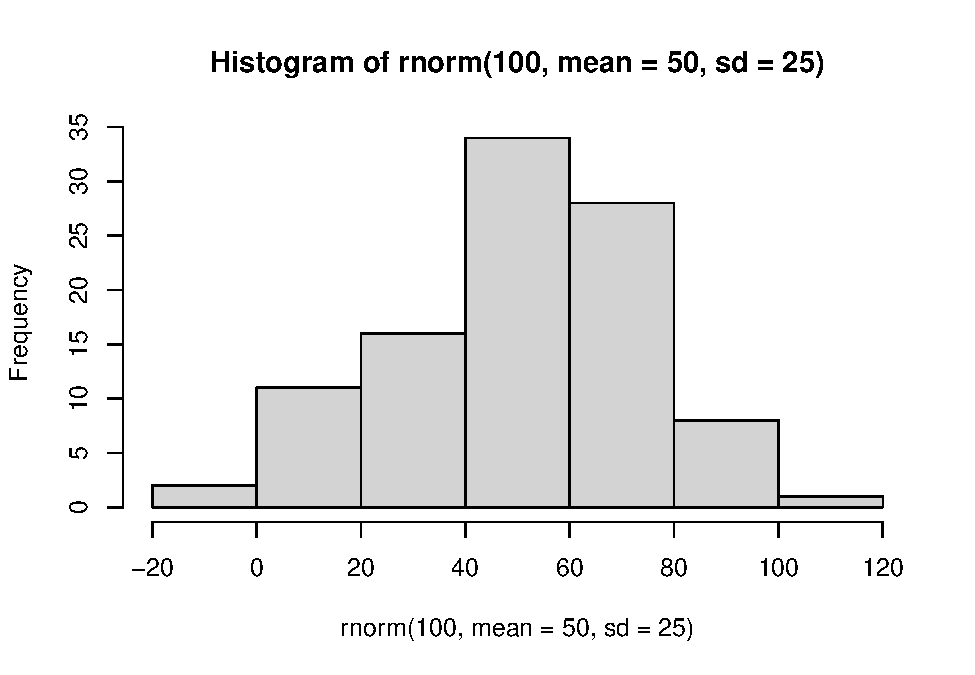
\includegraphics{Statistics_Lab_files/figure-latex/unnamed-chunk-34-1.pdf}

You just made R sample 100 numbers, and then plot the results in a histogram. Pretty neat. We'll be doing some of this later in the course, where get R to make fake data for us, and then we learn to think about how data behaves under different kinds of assumptions.

For now, let's do something that might be a little bit more interesting\ldots what movies are going to be filming in NYC? It turns out that NYC makes a lot of data about a lot things open and free for anyone to download and look at. This is the NYC Open Data website: \url{https://opendata.cityofnewyork.us}. I searched through the data, and found a data file that lists the locations of film permits for shooting movies all throughout the Burroughs. There are multiple ways to load this data into R.

\begin{enumerate}
\def\labelenumi{\arabic{enumi}.}
\tightlist
\item
  If you have downloaded the \href{https://github.com/CrumpLab/statisticsLab/raw/master/RMarkdownsLab.zip}{RMarkdownsLab.zip} file, then you already have the data file in the data folder. Assuming you are working in your main directory (your .rmd file is saved in the main folder that contains both the data and template folders), then use the following commands to load the data.
\end{enumerate}

\begin{Shaded}
\begin{Highlighting}[]
\FunctionTok{library}\NormalTok{(data.table)}
\NormalTok{nyc\_films }\OtherTok{\textless{}{-}}\FunctionTok{fread}\NormalTok{(}\StringTok{"data/Film\_Permits.csv"}\NormalTok{)}
\end{Highlighting}
\end{Shaded}

\begin{enumerate}
\def\labelenumi{\arabic{enumi}.}
\setcounter{enumi}{1}
\tightlist
\item
  If the above method doesn't work, you can try loading the data from the course website using:
\end{enumerate}

\begin{Shaded}
\begin{Highlighting}[]
\FunctionTok{library}\NormalTok{(data.table)}
\NormalTok{nyc\_films }\OtherTok{\textless{}{-}} \FunctionTok{fread}\NormalTok{(}\StringTok{"https://raw.githubusercontent.com/CrumpLab/statisticsLab/master/data/Film\_Permits.csv"}\NormalTok{)}
\end{Highlighting}
\end{Shaded}

If you are having issues getting the data loaded, then talk to your lab instructor

\hypertarget{look-at-the-data}{%
\subsection{Look at the data}\label{look-at-the-data}}

You will be downloading and analyzing all kinds of data files this semester. We will follow the very same steps every time. The steps are to load the data, then look at it. You want to see what you've got.

In R-studio, you will now see a variable called \texttt{nyc\_films} in the top right-hand corner of the screen, in the environment tab. If you click this thing, it will show you the contents of the data in a new window. The data is stored in something we call a \texttt{data\ frame}. It's R lingo, for the thing that contains the data. Notice is a square, with rows going across, and columns going up and down. It looks kind of like an excel spreadsheet if you are familiar with Excel.

It's useful to know you can look at the data frame this way if you need to. But, this data frame is really big, it has 50,728 rows of data. That's a lot too much to look at.

\hypertarget{summarytools}{%
\subsubsection{summarytools}\label{summarytools}}

The summarytools packages give a quick way to summarize all of the data in a data frame. Here's how. When you run this code you will see the summary in the viewer on the bottom right hand side. There's a little browser button (arrow on top of little window) that you can click to expand and see the whole thing in a browser.

\begin{Shaded}
\begin{Highlighting}[]
\FunctionTok{library}\NormalTok{(summarytools)}
\FunctionTok{view}\NormalTok{(}\FunctionTok{dfSummary}\NormalTok{(nyc\_films))}
\end{Highlighting}
\end{Shaded}

That is super helpful, but it's still a lot to look at. Because there is so much data here, it's pretty much mind-boggling to start thinking about what to do with it.

\hypertarget{make-plots-to-answer-questions}{%
\subsection{Make Plots to answer questions}\label{make-plots-to-answer-questions}}

Let's walk through a couple questions we might have about this data. We can see that there were 50,728 film permits made. We can also see that there are different columns telling us information about each of the film permits. For example, the \texttt{Borough} column lists the Borough for each request, whether it was made for: Manhattan, Brooklyn, Bronx, Queen's, or Staten Island. Now we can ask our first question, and learn how to do some plotting in R.

\hypertarget{where-are-the-most-film-permits-being-requested}{%
\subsubsection{Where are the most film permits being requested?}\label{where-are-the-most-film-permits-being-requested}}

Do you have any guesses? Is it Manhattan, or Brooklyn, of the Bronx? Or Queen's or Staten Island? We can find out by plotting the data using a bar plot. We just need to count how many film permits are made in each borough, and then make different bars represent the the counts.

First, we do the counting in R. Run the following code.

\begin{Shaded}
\begin{Highlighting}[]
\FunctionTok{library}\NormalTok{(dplyr)}

\NormalTok{counts }\OtherTok{\textless{}{-}}\NormalTok{ nyc\_films }\SpecialCharTok{\%\textgreater{}\%}
          \FunctionTok{group\_by}\NormalTok{(Borough) }\SpecialCharTok{\%\textgreater{}\%}
          \FunctionTok{summarize}\NormalTok{(}\AttributeTok{count\_of\_permits =} \FunctionTok{length}\NormalTok{(Borough))}
\end{Highlighting}
\end{Shaded}

The above grouped the data by each of the five Borough's, and then counted the number of times each Borough occurred (using the \texttt{length} function). The result is a new variable called \texttt{count}. I chose to name this variable \texttt{count}. You can see that it is now displayed in the top-right hand corned in the environment tab. If you gave \texttt{count} a different name, like \texttt{muppets}, then it would be named what you called it.

If you click on the \texttt{counts} variable, you will see the five boroughs listed, along with the counts for how many film permits were requested in each Borough. These are the numbers that we want to plot in a graph.

We do the plot using a fantastic package called \texttt{ggplot2}. It is very powerful once you get the hand of it, and when you do, you will be able to make all sorts of interesting graphs. Here's the code to make the plot

\begin{Shaded}
\begin{Highlighting}[]
\FunctionTok{library}\NormalTok{(ggplot2)}

\FunctionTok{ggplot}\NormalTok{(counts, }\FunctionTok{aes}\NormalTok{(}\AttributeTok{x =}\NormalTok{ Borough, }\AttributeTok{y =}\NormalTok{ count\_of\_permits )) }\SpecialCharTok{+}
  \FunctionTok{geom\_bar}\NormalTok{(}\AttributeTok{stat=}\StringTok{"identity"}\NormalTok{)}
\end{Highlighting}
\end{Shaded}

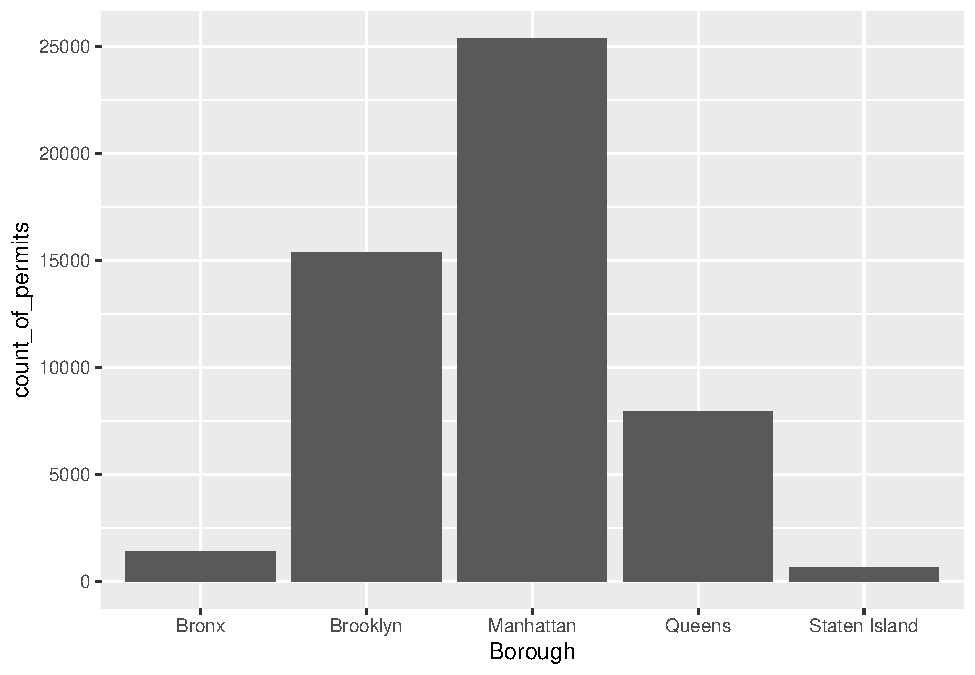
\includegraphics{Statistics_Lab_files/figure-latex/1borough-1.pdf}

There it is, we're done here! We can easily look at this graph, and answer our question. Most of the film permits were requested in Manhattan, followed by Brooklyn, then Queen's, the Bronx, and finally Staten Island.

\hypertarget{what-kind-of-films-are-being-made-what-is-the-category}{%
\subsubsection{What kind of ``films'' are being made, what is the category?}\label{what-kind-of-films-are-being-made-what-is-the-category}}

We think you might be skeptical of what you are doing here, copying and pasting things. Soon you'll see just how fast you can do things by copying and pasting, and make a few little changes. Let's quickly ask another question about what kinds of films are being made. The column \texttt{Category}, gives us some information about that. Let's just copy paste the code we already made, and see what kinds of categories the films fall into. See if you can tell what I changed in the code to make this work, I'll do it all at once:

\begin{Shaded}
\begin{Highlighting}[]
\NormalTok{counts }\OtherTok{\textless{}{-}}\NormalTok{ nyc\_films }\SpecialCharTok{\%\textgreater{}\%}
          \FunctionTok{group\_by}\NormalTok{(Category) }\SpecialCharTok{\%\textgreater{}\%}
          \FunctionTok{summarize}\NormalTok{(}\AttributeTok{count\_of\_permits =} \FunctionTok{length}\NormalTok{(Category))}

\FunctionTok{ggplot}\NormalTok{(counts, }\FunctionTok{aes}\NormalTok{(}\AttributeTok{x =}\NormalTok{ Category, }\AttributeTok{y =}\NormalTok{ count\_of\_permits )) }\SpecialCharTok{+}
  \FunctionTok{geom\_bar}\NormalTok{(}\AttributeTok{stat=}\StringTok{"identity"}\NormalTok{)}\SpecialCharTok{+} 
  \FunctionTok{theme}\NormalTok{(}\AttributeTok{axis.text.x =} \FunctionTok{element\_text}\NormalTok{(}\AttributeTok{angle =} \DecValTok{90}\NormalTok{, }\AttributeTok{hjust =} \DecValTok{1}\NormalTok{))}
\end{Highlighting}
\end{Shaded}

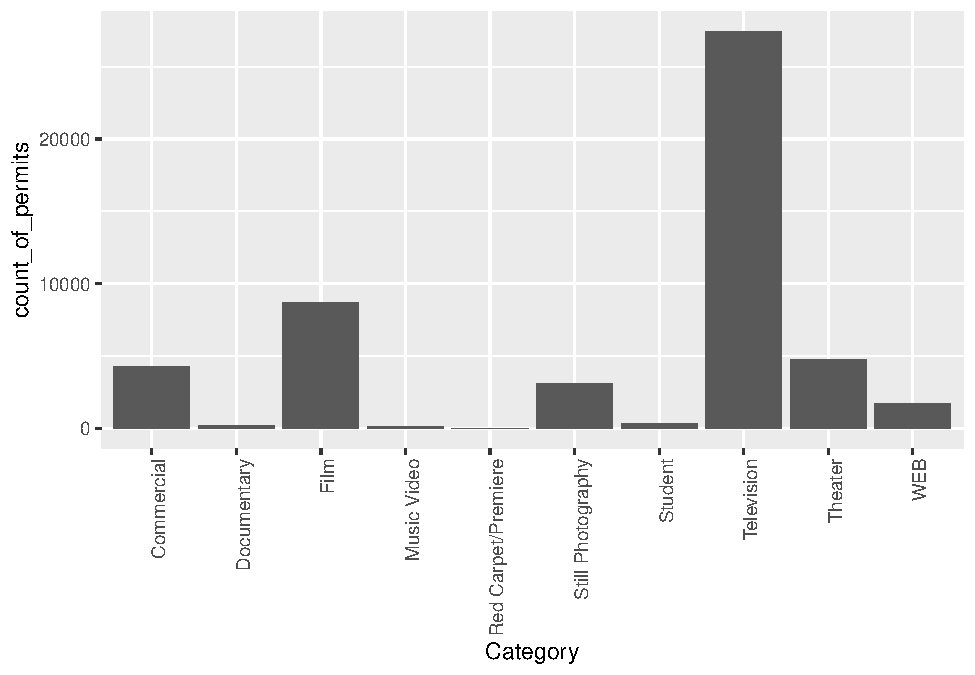
\includegraphics{Statistics_Lab_files/figure-latex/1category-1.pdf}

OK, so this figure might look a bit weird because the labels on the bottom are running into each other. We'll fix that in a bit. First, let's notice the changes.

\begin{enumerate}
\def\labelenumi{\arabic{enumi}.}
\item
  I changed \texttt{Borough} to \texttt{Category}. That was the main thing
\item
  I left out a bunch of things from before. None of the \texttt{library()} commands are used again, and I didn't re-run the very early code to get the data. R already has those things in it's memory, so we don't need to do that first. If you ever clear the memory of R, then you will need to reload those things. First-things come first.
\end{enumerate}

Fine, so how do we fix the graph? Good question. To be honest, I don't know right now. I totally forgot how. But, I know ggplot2 can do this, and I'm going to Google it, right now. Then I'm going to find the answer, and use it here. The googling of your questions is a fine way to learn. It's what everybody does these days\ldots.{[}goes to Google\ldots{]}.

Found it, actually found a lot of ways to do this. The trick is to add the last line. I just copy-pasted it from the solution I found on \href{https://stackoverflow.com/questions/1330989/rotating-and-spacing-axis-labels-in-ggplot2}{stack overflow} (you will become friend's with stack overflow, there are many solutions there to all of your questions)

\begin{Shaded}
\begin{Highlighting}[]
\NormalTok{counts }\OtherTok{\textless{}{-}}\NormalTok{ nyc\_films }\SpecialCharTok{\%\textgreater{}\%}
          \FunctionTok{group\_by}\NormalTok{(Category) }\SpecialCharTok{\%\textgreater{}\%}
          \FunctionTok{summarize}\NormalTok{(}\AttributeTok{count\_of\_permits =} \FunctionTok{length}\NormalTok{(Category))}

\FunctionTok{ggplot}\NormalTok{(counts, }\FunctionTok{aes}\NormalTok{(}\AttributeTok{x =}\NormalTok{ Category, }\AttributeTok{y =}\NormalTok{ count\_of\_permits )) }\SpecialCharTok{+}
  \FunctionTok{geom\_bar}\NormalTok{(}\AttributeTok{stat=}\StringTok{"identity"}\NormalTok{)}\SpecialCharTok{+} 
  \FunctionTok{theme}\NormalTok{(}\AttributeTok{axis.text.x =} \FunctionTok{element\_text}\NormalTok{(}\AttributeTok{angle =} \DecValTok{90}\NormalTok{, }\AttributeTok{hjust =} \DecValTok{1}\NormalTok{))}
\end{Highlighting}
\end{Shaded}

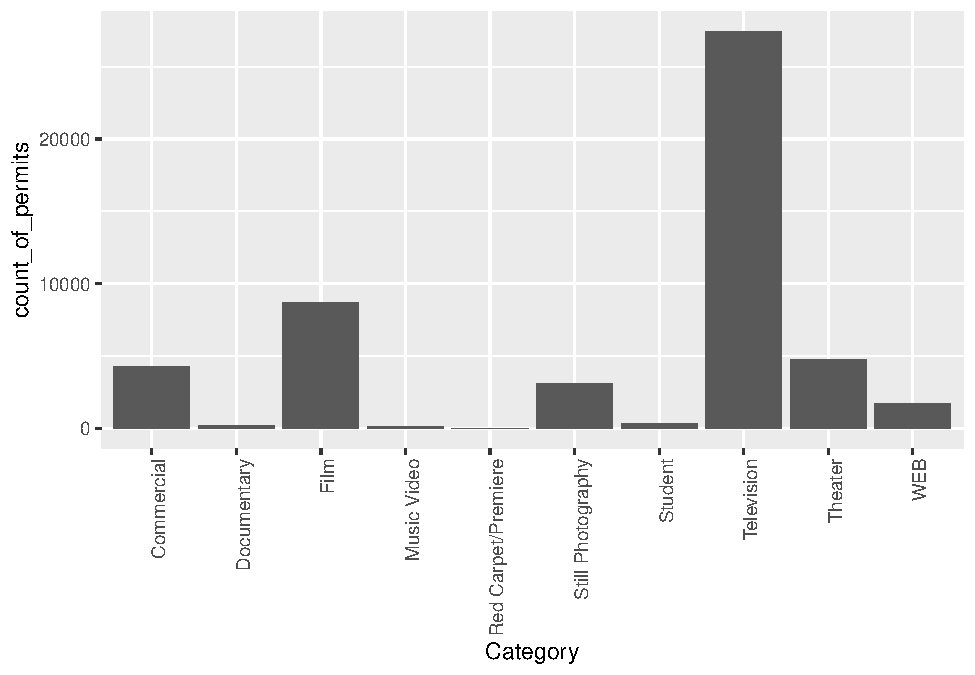
\includegraphics{Statistics_Lab_files/figure-latex/1categoryB-1.pdf}

\hypertarget{ggplot2-basics}{%
\subsection{ggplot2 basics}\label{ggplot2-basics}}

Before we go further, I want to point out some basic properties of ggplot2, just to give you a sense of how it is working. This will make more sense in a few weeks, so come back here to remind yourself. We'll do just a bit a basics, and then move on to making more graphs, by copying and pasting.

The ggplot function uses layers. Layers you say? What are these layers? Well, it draws things from the bottom up. It lays down one layer of graphics, then you can keep adding on top, drawing more things. So the idea is something like: Layer 1 + Layer 2 + Layer 3, and so on. If you want Layer 3 to be Layer 2, then you just switch them in the code.

Here is a way of thinking about ggplot code

\begin{verbatim}
ggplot(name_of_data, aes(x = name_of_x_variable, y = name_of_y_variable)) +
    geom_layer()+
    geom_layer()+
    geom_layer()
\end{verbatim}

What I want you to focus on in the above description is the \(+\) signs. What we are doing with the plus signs is adding layers to plot. The layers get added in the order that they are written. If you look back to our previous code, you will see we add a \texttt{geom\_bar} layer, then we added another layer to change the rotation of the words on the x-axis. This is how it works.

BUT WAIT? How am I supposed to know what to add? This is nuts! We know. You're not supposed to know just yet, how could you? We'll give you lots of examples where you can copy and paste, and they will work. That's how you'll learn. If you really want to read the \href{https://ggplot2.tidyverse.org/reference/index.html}{help manual} you can do that too. It's on the ggplot2 website. This will become useful after you already know what you are doing, before that, it will probably just seem very confusing. However, it is pretty neat to look and \href{http://www.ggplot2-exts.org/gallery/}{see all of the different things you can do}, it's very powerful.

For now, let's the get the hang of adding things to the graph that let us change some stuff we might want to change. For example, how do you add a title? Or change the labels on the axes? Or add different colors, or change the font-size, or change the background? You can change all of these things by adding different lines to the existing code.

\hypertarget{ylab-changes-y-label}{%
\subsubsection{ylab() changes y label}\label{ylab-changes-y-label}}

The last graph had \texttt{count\_of\_permits} as the label on the y-axis. That doesn't look right. ggplot2 automatically took the label from the column, and made it be the name on the y-axis. We can change that by adding \texttt{ylab("what\ we\ want")}. We do this by adding a \(+\) to the last line, then adding \texttt{ylab()}

\begin{Shaded}
\begin{Highlighting}[]
\FunctionTok{ggplot}\NormalTok{(counts, }\FunctionTok{aes}\NormalTok{(}\AttributeTok{x =}\NormalTok{ Category, }\AttributeTok{y =}\NormalTok{ count\_of\_permits )) }\SpecialCharTok{+}
  \FunctionTok{geom\_bar}\NormalTok{(}\AttributeTok{stat=}\StringTok{"identity"}\NormalTok{) }\SpecialCharTok{+} 
  \FunctionTok{theme}\NormalTok{(}\AttributeTok{axis.text.x =} \FunctionTok{element\_text}\NormalTok{(}\AttributeTok{angle =} \DecValTok{90}\NormalTok{, }\AttributeTok{hjust =} \DecValTok{1}\NormalTok{)) }\SpecialCharTok{+}
  \FunctionTok{ylab}\NormalTok{(}\StringTok{"Number of Film Permits"}\NormalTok{)}
\end{Highlighting}
\end{Shaded}

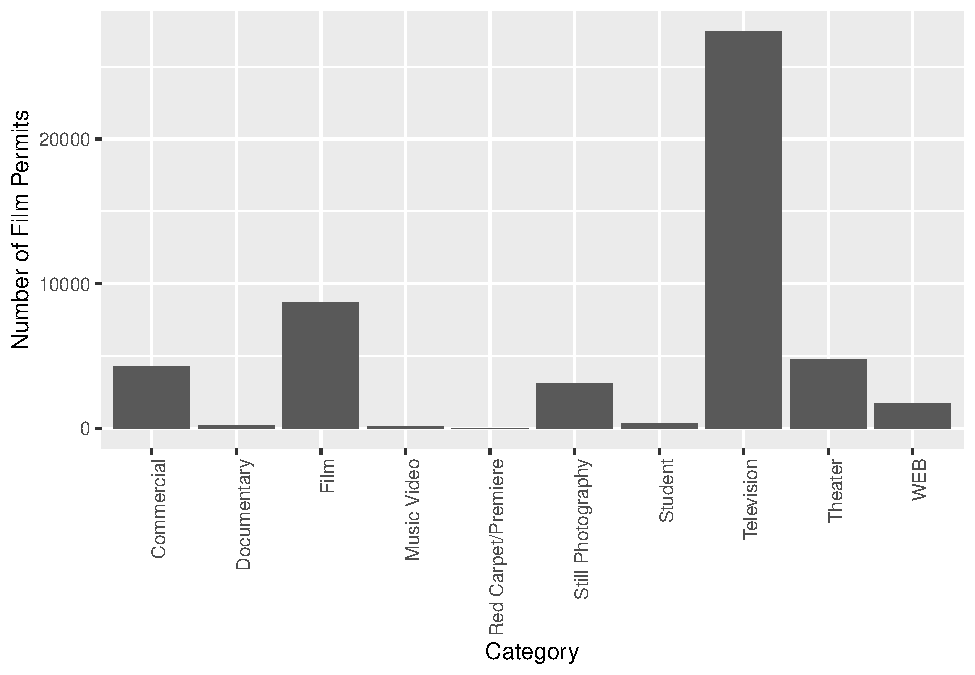
\includegraphics{Statistics_Lab_files/figure-latex/1categoryC-1.pdf}

\hypertarget{xlab-changes-x-label}{%
\subsubsection{xlab() changes x label}\label{xlab-changes-x-label}}

Let's slightly modify the x label too:

\begin{Shaded}
\begin{Highlighting}[]
\FunctionTok{ggplot}\NormalTok{(counts, }\FunctionTok{aes}\NormalTok{(}\AttributeTok{x =}\NormalTok{ Category, }\AttributeTok{y =}\NormalTok{ count\_of\_permits )) }\SpecialCharTok{+}
  \FunctionTok{geom\_bar}\NormalTok{(}\AttributeTok{stat=}\StringTok{"identity"}\NormalTok{) }\SpecialCharTok{+} 
  \FunctionTok{theme}\NormalTok{(}\AttributeTok{axis.text.x =} \FunctionTok{element\_text}\NormalTok{(}\AttributeTok{angle =} \DecValTok{90}\NormalTok{, }\AttributeTok{hjust =} \DecValTok{1}\NormalTok{)) }\SpecialCharTok{+}
  \FunctionTok{ylab}\NormalTok{(}\StringTok{"Number of Film Permits"}\NormalTok{) }\SpecialCharTok{+} 
  \FunctionTok{xlab}\NormalTok{(}\StringTok{"Category of film"}\NormalTok{)}
\end{Highlighting}
\end{Shaded}

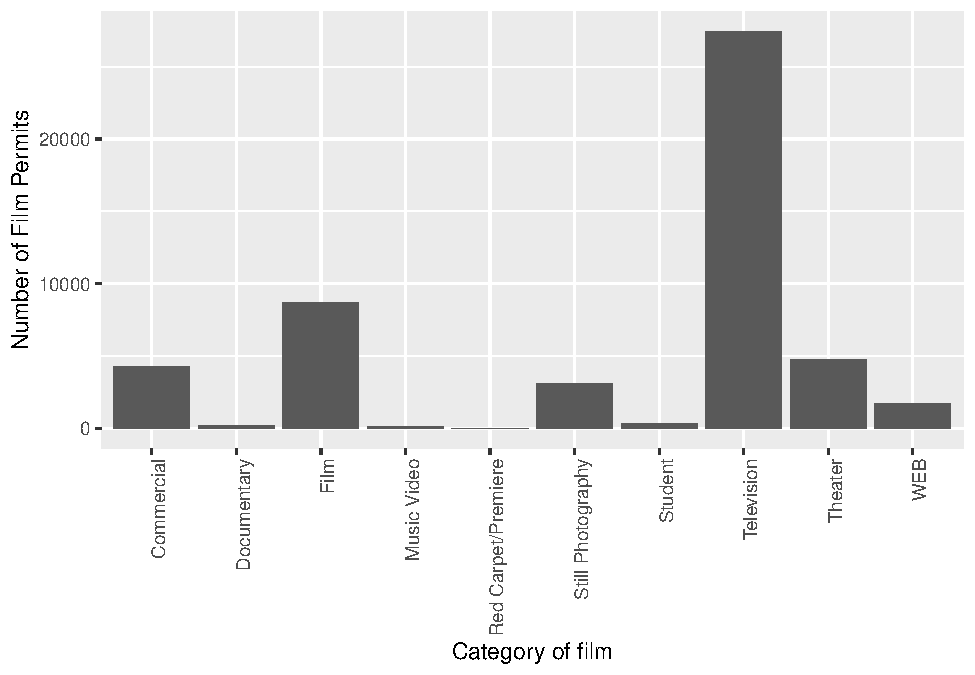
\includegraphics{Statistics_Lab_files/figure-latex/1categoryD-1.pdf}

\hypertarget{ggtitle-adds-title}{%
\subsubsection{ggtitle() adds title}\label{ggtitle-adds-title}}

Let's give our graph a title

\begin{Shaded}
\begin{Highlighting}[]
\FunctionTok{ggplot}\NormalTok{(counts, }\FunctionTok{aes}\NormalTok{(}\AttributeTok{x =}\NormalTok{ Category, }\AttributeTok{y =}\NormalTok{ count\_of\_permits )) }\SpecialCharTok{+}
  \FunctionTok{geom\_bar}\NormalTok{(}\AttributeTok{stat=}\StringTok{"identity"}\NormalTok{) }\SpecialCharTok{+} 
  \FunctionTok{theme}\NormalTok{(}\AttributeTok{axis.text.x =} \FunctionTok{element\_text}\NormalTok{(}\AttributeTok{angle =} \DecValTok{90}\NormalTok{, }\AttributeTok{hjust =} \DecValTok{1}\NormalTok{)) }\SpecialCharTok{+}
  \FunctionTok{ylab}\NormalTok{(}\StringTok{"Number of Film Permits"}\NormalTok{) }\SpecialCharTok{+} 
  \FunctionTok{xlab}\NormalTok{(}\StringTok{"Category of film"}\NormalTok{) }\SpecialCharTok{+}
  \FunctionTok{ggtitle}\NormalTok{(}\StringTok{"Number of Film permits in NYC by Category"}\NormalTok{)}
\end{Highlighting}
\end{Shaded}

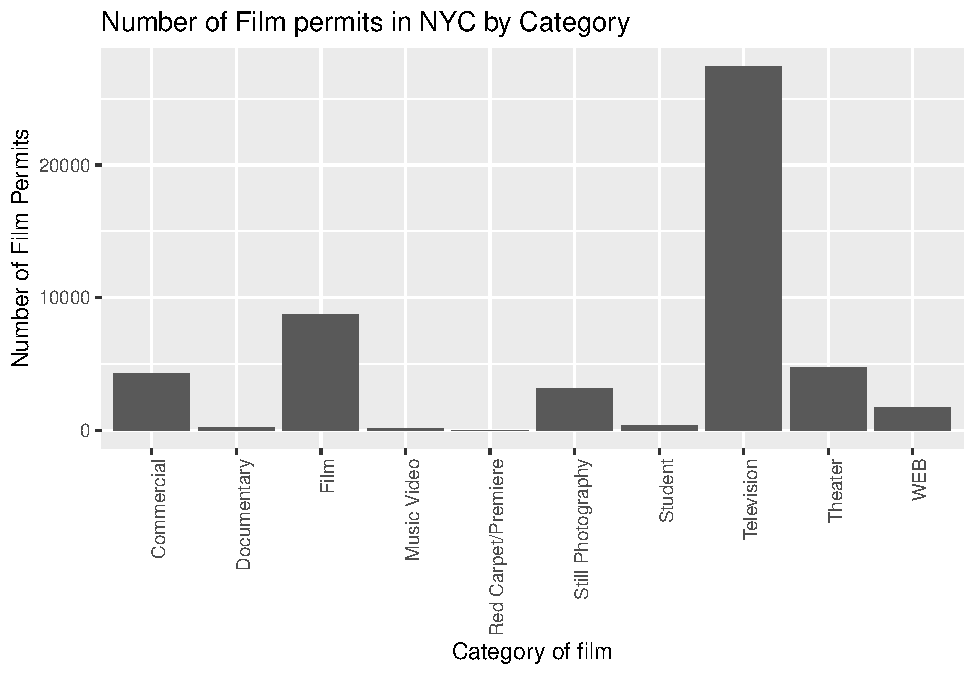
\includegraphics{Statistics_Lab_files/figure-latex/1categoryE-1.pdf}

\hypertarget{color-adds-color}{%
\subsubsection{color adds color}\label{color-adds-color}}

Let's make the bars different colors. To do this, we add new code to the inside of the \texttt{aes()} part:

\begin{Shaded}
\begin{Highlighting}[]
\FunctionTok{ggplot}\NormalTok{(counts, }\FunctionTok{aes}\NormalTok{(}\AttributeTok{x =}\NormalTok{ Category, }\AttributeTok{y =}\NormalTok{ count\_of\_permits, }\AttributeTok{color=}\NormalTok{Category )) }\SpecialCharTok{+}
  \FunctionTok{geom\_bar}\NormalTok{(}\AttributeTok{stat=}\StringTok{"identity"}\NormalTok{) }\SpecialCharTok{+} 
  \FunctionTok{theme}\NormalTok{(}\AttributeTok{axis.text.x =} \FunctionTok{element\_text}\NormalTok{(}\AttributeTok{angle =} \DecValTok{90}\NormalTok{, }\AttributeTok{hjust =} \DecValTok{1}\NormalTok{)) }\SpecialCharTok{+}
  \FunctionTok{ylab}\NormalTok{(}\StringTok{"Number of Film Permits"}\NormalTok{) }\SpecialCharTok{+} 
  \FunctionTok{xlab}\NormalTok{(}\StringTok{"Category of film"}\NormalTok{) }\SpecialCharTok{+}
  \FunctionTok{ggtitle}\NormalTok{(}\StringTok{"Number of Film permits in NYC by Category"}\NormalTok{)}
\end{Highlighting}
\end{Shaded}

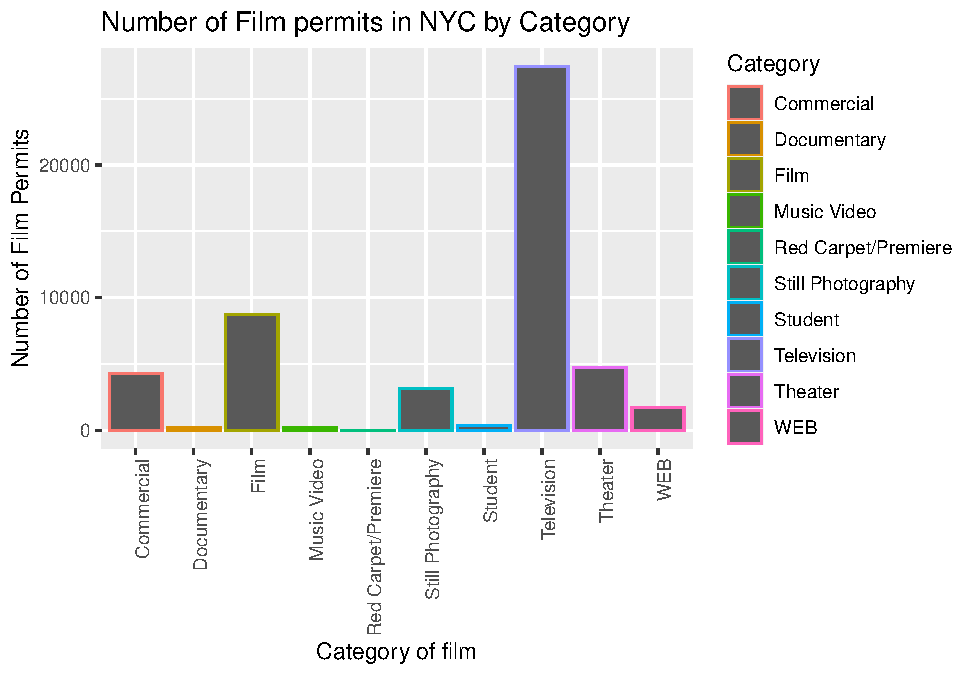
\includegraphics{Statistics_Lab_files/figure-latex/1categoryF-1.pdf}

\hypertarget{fill-fills-in-color}{%
\subsubsection{fill fills in color}\label{fill-fills-in-color}}

Let's make the bars different colors. To do this, we add new code to the inside of the \texttt{aes()} part\ldots Notice I've started using new lines to make the code more readable.

\begin{Shaded}
\begin{Highlighting}[]
\FunctionTok{ggplot}\NormalTok{(counts, }\FunctionTok{aes}\NormalTok{(}\AttributeTok{x =}\NormalTok{ Category, }\AttributeTok{y =}\NormalTok{ count\_of\_permits, }
                   \AttributeTok{color=}\NormalTok{Category, }
                   \AttributeTok{fill=}\NormalTok{ Category )) }\SpecialCharTok{+}
  \FunctionTok{geom\_bar}\NormalTok{(}\AttributeTok{stat=}\StringTok{"identity"}\NormalTok{) }\SpecialCharTok{+} 
  \FunctionTok{theme}\NormalTok{(}\AttributeTok{axis.text.x =} \FunctionTok{element\_text}\NormalTok{(}\AttributeTok{angle =} \DecValTok{90}\NormalTok{, }\AttributeTok{hjust =} \DecValTok{1}\NormalTok{)) }\SpecialCharTok{+}
  \FunctionTok{ylab}\NormalTok{(}\StringTok{"Number of Film Permits"}\NormalTok{) }\SpecialCharTok{+} 
  \FunctionTok{xlab}\NormalTok{(}\StringTok{"Category of film"}\NormalTok{) }\SpecialCharTok{+}
  \FunctionTok{ggtitle}\NormalTok{(}\StringTok{"Number of Film permits in NYC by Category"}\NormalTok{)}
\end{Highlighting}
\end{Shaded}

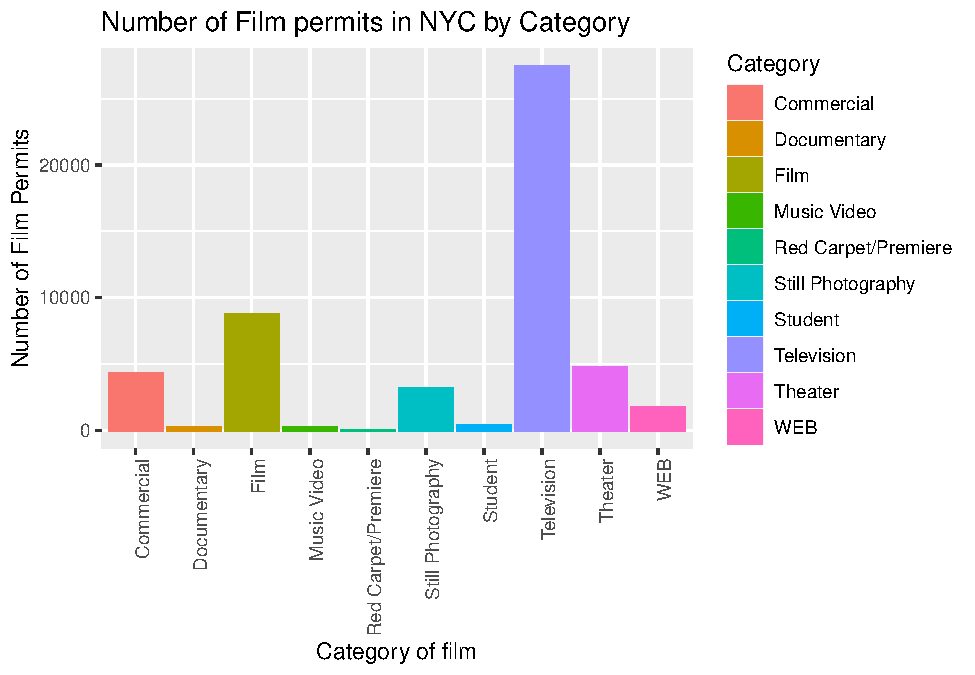
\includegraphics{Statistics_Lab_files/figure-latex/1categoryG-1.pdf}

\hypertarget{get-rid-of-the-legend}{%
\subsubsection{get rid of the legend}\label{get-rid-of-the-legend}}

Sometimes you just don't want the legend on the side, to remove it add

\texttt{theme(legend.position="none")}

\begin{Shaded}
\begin{Highlighting}[]
\FunctionTok{ggplot}\NormalTok{(counts, }\FunctionTok{aes}\NormalTok{(}\AttributeTok{x =}\NormalTok{ Category, }\AttributeTok{y =}\NormalTok{ count\_of\_permits, }
                   \AttributeTok{color=}\NormalTok{Category, }
                   \AttributeTok{fill=}\NormalTok{ Category )) }\SpecialCharTok{+}
  \FunctionTok{geom\_bar}\NormalTok{(}\AttributeTok{stat=}\StringTok{"identity"}\NormalTok{) }\SpecialCharTok{+} 
  \FunctionTok{theme}\NormalTok{(}\AttributeTok{axis.text.x =} \FunctionTok{element\_text}\NormalTok{(}\AttributeTok{angle =} \DecValTok{90}\NormalTok{, }\AttributeTok{hjust =} \DecValTok{1}\NormalTok{)) }\SpecialCharTok{+}
  \FunctionTok{ylab}\NormalTok{(}\StringTok{"Number of Film Permits"}\NormalTok{) }\SpecialCharTok{+} 
  \FunctionTok{xlab}\NormalTok{(}\StringTok{"Category of film"}\NormalTok{) }\SpecialCharTok{+}
  \FunctionTok{ggtitle}\NormalTok{(}\StringTok{"Number of Film permits in NYC by Category"}\NormalTok{) }\SpecialCharTok{+}
  \FunctionTok{theme}\NormalTok{(}\AttributeTok{legend.position=}\StringTok{"none"}\NormalTok{)}
\end{Highlighting}
\end{Shaded}

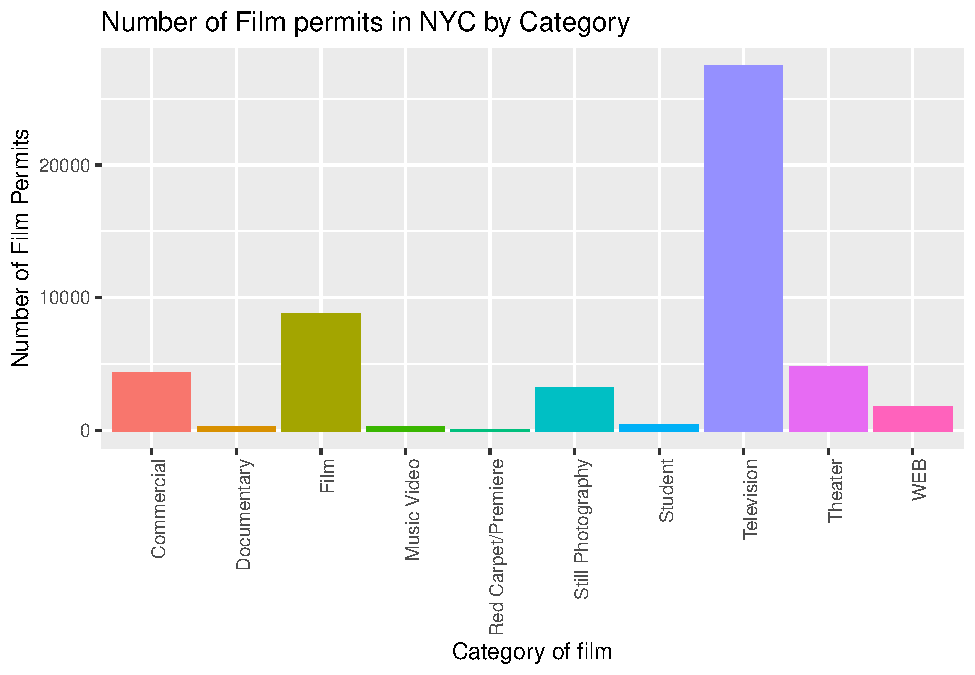
\includegraphics{Statistics_Lab_files/figure-latex/1categoryH-1.pdf}

\hypertarget{theme_classic-makes-white-background}{%
\subsubsection{theme\_classic() makes white background}\label{theme_classic-makes-white-background}}

The rest is often just visual preference. For example, the graph above has this grey grid behind the bars. For a clean classic no nonsense look, use \texttt{theme\_classic()} to take away the grid.

\begin{Shaded}
\begin{Highlighting}[]
\FunctionTok{ggplot}\NormalTok{(counts, }\FunctionTok{aes}\NormalTok{(}\AttributeTok{x =}\NormalTok{ Category, }\AttributeTok{y =}\NormalTok{ count\_of\_permits, }
                   \AttributeTok{color=}\NormalTok{Category, }
                   \AttributeTok{fill=}\NormalTok{ Category )) }\SpecialCharTok{+}
  \FunctionTok{geom\_bar}\NormalTok{(}\AttributeTok{stat=}\StringTok{"identity"}\NormalTok{) }\SpecialCharTok{+} 
  \FunctionTok{theme}\NormalTok{(}\AttributeTok{axis.text.x =} \FunctionTok{element\_text}\NormalTok{(}\AttributeTok{angle =} \DecValTok{90}\NormalTok{, }\AttributeTok{hjust =} \DecValTok{1}\NormalTok{)) }\SpecialCharTok{+}
  \FunctionTok{ylab}\NormalTok{(}\StringTok{"Number of Film Permits"}\NormalTok{) }\SpecialCharTok{+} 
  \FunctionTok{xlab}\NormalTok{(}\StringTok{"Category of film"}\NormalTok{) }\SpecialCharTok{+}
  \FunctionTok{ggtitle}\NormalTok{(}\StringTok{"Number of Film permits in NYC by Category"}\NormalTok{) }\SpecialCharTok{+}
  \FunctionTok{theme}\NormalTok{(}\AttributeTok{legend.position=}\StringTok{"none"}\NormalTok{) }\SpecialCharTok{+}
  \FunctionTok{theme\_classic}\NormalTok{()}
\end{Highlighting}
\end{Shaded}

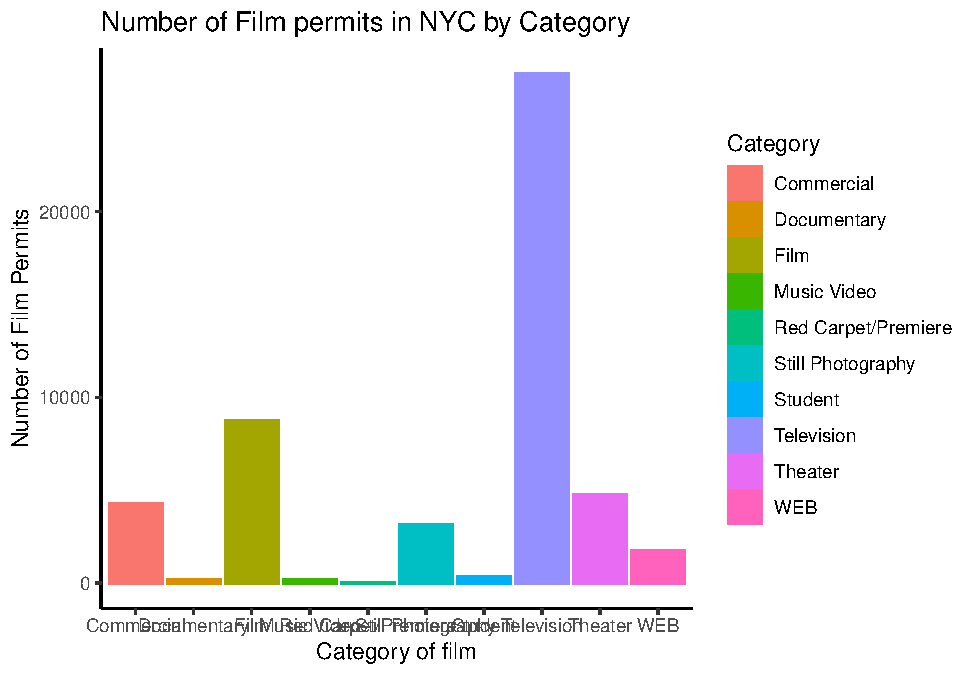
\includegraphics{Statistics_Lab_files/figure-latex/1categoryI-1.pdf}

\hypertarget{sometimes-layer-order-matters}{%
\subsubsection{Sometimes layer order matters}\label{sometimes-layer-order-matters}}

Interesting, \texttt{theme\_classic()} is misbehaving a little bit. It looks like we have some of our layer out of order, let's re-order. I just moved \texttt{theme\_classic()} to just underneath the \texttt{geom\_bar()} line. Now everything get's drawn properly.

\begin{Shaded}
\begin{Highlighting}[]
\FunctionTok{ggplot}\NormalTok{(counts, }\FunctionTok{aes}\NormalTok{(}\AttributeTok{x =}\NormalTok{ Category, }\AttributeTok{y =}\NormalTok{ count\_of\_permits, }
                   \AttributeTok{color=}\NormalTok{Category, }
                   \AttributeTok{fill=}\NormalTok{ Category )) }\SpecialCharTok{+}
  \FunctionTok{geom\_bar}\NormalTok{(}\AttributeTok{stat=}\StringTok{"identity"}\NormalTok{) }\SpecialCharTok{+} 
  \FunctionTok{theme\_classic}\NormalTok{() }\SpecialCharTok{+}
  \FunctionTok{theme}\NormalTok{(}\AttributeTok{axis.text.x =} \FunctionTok{element\_text}\NormalTok{(}\AttributeTok{angle =} \DecValTok{90}\NormalTok{, }\AttributeTok{hjust =} \DecValTok{1}\NormalTok{)) }\SpecialCharTok{+}
  \FunctionTok{ylab}\NormalTok{(}\StringTok{"Number of Film Permits"}\NormalTok{) }\SpecialCharTok{+} 
  \FunctionTok{xlab}\NormalTok{(}\StringTok{"Category of film"}\NormalTok{) }\SpecialCharTok{+}
  \FunctionTok{ggtitle}\NormalTok{(}\StringTok{"Number of Film permits in NYC by Category"}\NormalTok{) }\SpecialCharTok{+}
  \FunctionTok{theme}\NormalTok{(}\AttributeTok{legend.position=}\StringTok{"none"}\NormalTok{) }
\end{Highlighting}
\end{Shaded}

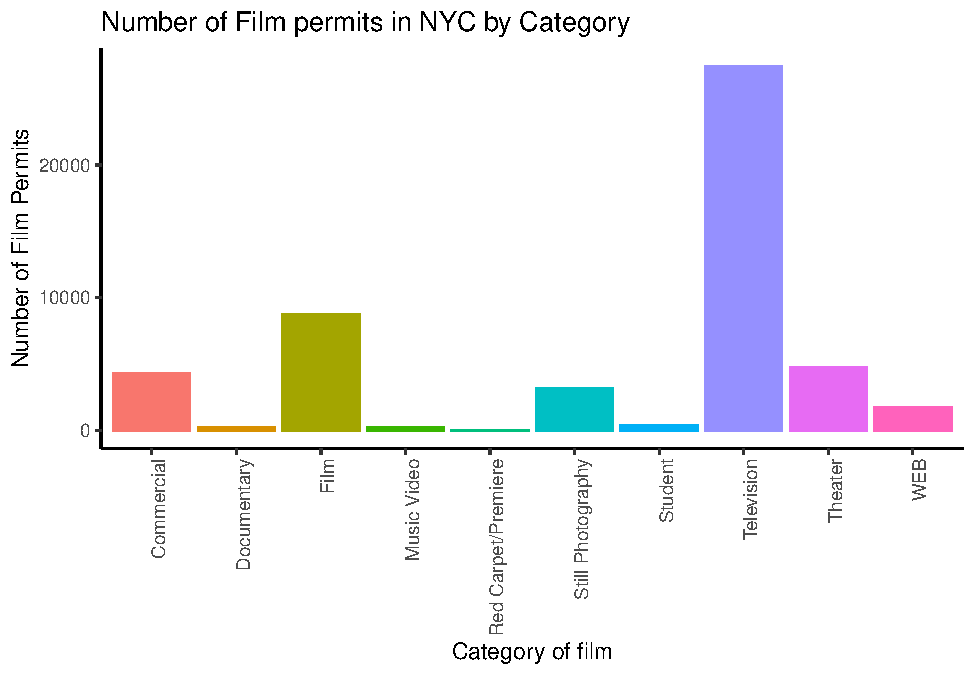
\includegraphics{Statistics_Lab_files/figure-latex/1categoryJ-1.pdf}

\hypertarget{font-size}{%
\subsubsection{Font-size}\label{font-size}}

Changing font-size is often something you want to do. ggplot2 can do this in different ways. I suggest using the \texttt{base\_size} option inside \texttt{theme\_classic()}. You set one number for the largest font size in the graph, and everything else gets scaled to fit with that that first number. It's really convenient. Look for the inside of \texttt{theme\_classic()}

\begin{Shaded}
\begin{Highlighting}[]
\FunctionTok{ggplot}\NormalTok{(counts, }\FunctionTok{aes}\NormalTok{(}\AttributeTok{x =}\NormalTok{ Category, }\AttributeTok{y =}\NormalTok{ count\_of\_permits, }
                   \AttributeTok{color=}\NormalTok{Category, }
                   \AttributeTok{fill=}\NormalTok{ Category )) }\SpecialCharTok{+}
  \FunctionTok{geom\_bar}\NormalTok{(}\AttributeTok{stat=}\StringTok{"identity"}\NormalTok{) }\SpecialCharTok{+} 
  \FunctionTok{theme\_classic}\NormalTok{(}\AttributeTok{base\_size =} \DecValTok{15}\NormalTok{) }\SpecialCharTok{+}
  \FunctionTok{theme}\NormalTok{(}\AttributeTok{axis.text.x =} \FunctionTok{element\_text}\NormalTok{(}\AttributeTok{angle =} \DecValTok{90}\NormalTok{, }\AttributeTok{hjust =} \DecValTok{1}\NormalTok{)) }\SpecialCharTok{+}
  \FunctionTok{ylab}\NormalTok{(}\StringTok{"Number of Film Permits"}\NormalTok{) }\SpecialCharTok{+} 
  \FunctionTok{xlab}\NormalTok{(}\StringTok{"Category of film"}\NormalTok{) }\SpecialCharTok{+}
  \FunctionTok{ggtitle}\NormalTok{(}\StringTok{"Number of Film permits in NYC by Category"}\NormalTok{) }\SpecialCharTok{+}
  \FunctionTok{theme}\NormalTok{(}\AttributeTok{legend.position=}\StringTok{"none"}\NormalTok{) }
\end{Highlighting}
\end{Shaded}

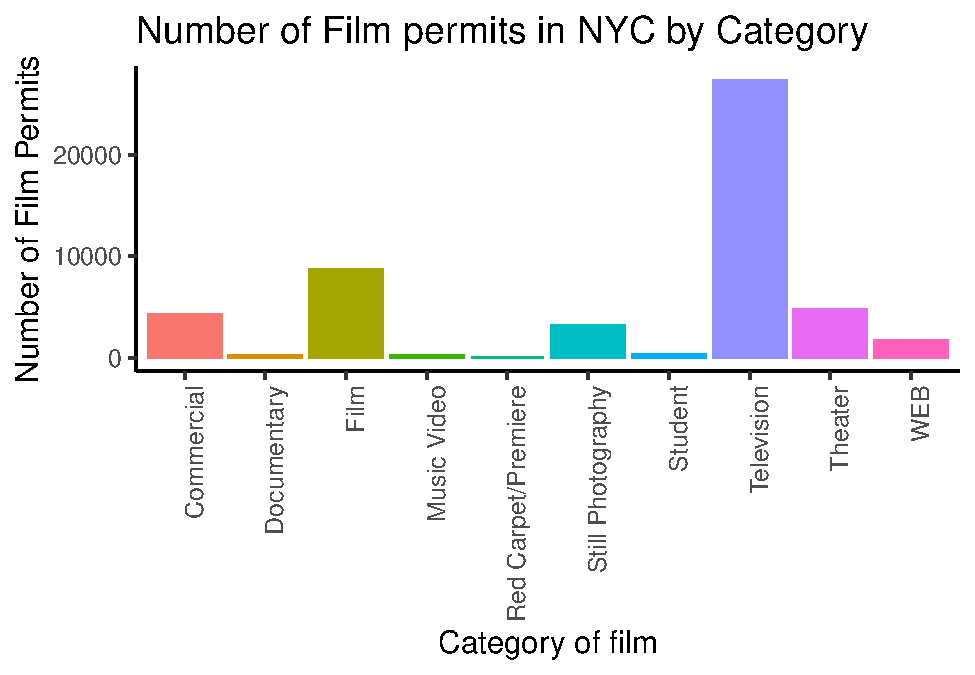
\includegraphics{Statistics_Lab_files/figure-latex/1categoryK-1.pdf}
or make things small\ldots{} just to see what happens

\begin{Shaded}
\begin{Highlighting}[]
\FunctionTok{ggplot}\NormalTok{(counts, }\FunctionTok{aes}\NormalTok{(}\AttributeTok{x =}\NormalTok{ Category, }\AttributeTok{y =}\NormalTok{ count\_of\_permits, }
                   \AttributeTok{color=}\NormalTok{Category, }
                   \AttributeTok{fill=}\NormalTok{ Category )) }\SpecialCharTok{+}
  \FunctionTok{geom\_bar}\NormalTok{(}\AttributeTok{stat=}\StringTok{"identity"}\NormalTok{) }\SpecialCharTok{+} 
  \FunctionTok{theme\_classic}\NormalTok{(}\AttributeTok{base\_size =} \DecValTok{10}\NormalTok{) }\SpecialCharTok{+}
  \FunctionTok{theme}\NormalTok{(}\AttributeTok{axis.text.x =} \FunctionTok{element\_text}\NormalTok{(}\AttributeTok{angle =} \DecValTok{90}\NormalTok{, }\AttributeTok{hjust =} \DecValTok{1}\NormalTok{)) }\SpecialCharTok{+}
  \FunctionTok{ylab}\NormalTok{(}\StringTok{"Number of Film Permits"}\NormalTok{) }\SpecialCharTok{+} 
  \FunctionTok{xlab}\NormalTok{(}\StringTok{"Category of film"}\NormalTok{) }\SpecialCharTok{+}
  \FunctionTok{ggtitle}\NormalTok{(}\StringTok{"Number of Film permits in NYC by Category"}\NormalTok{) }\SpecialCharTok{+}
  \FunctionTok{theme}\NormalTok{(}\AttributeTok{legend.position=}\StringTok{"none"}\NormalTok{) }
\end{Highlighting}
\end{Shaded}

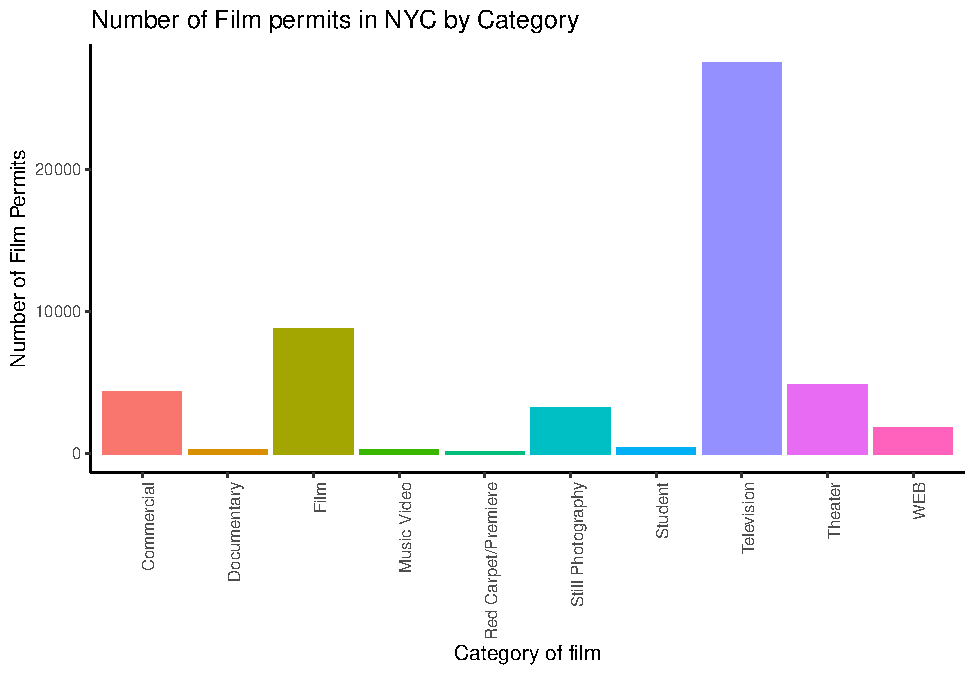
\includegraphics{Statistics_Lab_files/figure-latex/1categoryL-1.pdf}

\hypertarget{ggplot2-summary}{%
\subsubsection{ggplot2 summary}\label{ggplot2-summary}}

That's enough of the ggplot2 basics for now. You will discover that many things are possible with ggplot2. It is amazing. We are going to get back to answering some questions about the data with graphs. But, now that we have built the code to make the graphs, all we need to do is copy-paste, and make a few small changes, and boom, we have our graph.

\hypertarget{more-questions-about-nyc-films}{%
\subsection{More questions about NYC films}\label{more-questions-about-nyc-films}}

\hypertarget{what-are-the-sub-categories-of-films}{%
\subsubsection{What are the sub-categories of films?}\label{what-are-the-sub-categories-of-films}}

Notice the \texttt{nyc\_films} data frame also has a column for \texttt{SubCategoryName}. Let's see what's going on there with a quick plot.

\begin{Shaded}
\begin{Highlighting}[]
\CommentTok{\# get the counts (this is a comment it\textquotesingle{}s just here for you to read)}

\NormalTok{counts }\OtherTok{\textless{}{-}}\NormalTok{ nyc\_films }\SpecialCharTok{\%\textgreater{}\%}
          \FunctionTok{group\_by}\NormalTok{(SubCategoryName) }\SpecialCharTok{\%\textgreater{}\%}
          \FunctionTok{summarize}\NormalTok{(}\AttributeTok{count\_of\_permits =} \FunctionTok{length}\NormalTok{(SubCategoryName))}

\CommentTok{\# make the plot}

\FunctionTok{ggplot}\NormalTok{(counts, }\FunctionTok{aes}\NormalTok{(}\AttributeTok{x =}\NormalTok{ SubCategoryName, }\AttributeTok{y =}\NormalTok{ count\_of\_permits, }
                   \AttributeTok{color=}\NormalTok{SubCategoryName, }
                   \AttributeTok{fill=}\NormalTok{ SubCategoryName )) }\SpecialCharTok{+}
  \FunctionTok{geom\_bar}\NormalTok{(}\AttributeTok{stat=}\StringTok{"identity"}\NormalTok{) }\SpecialCharTok{+} 
  \FunctionTok{theme\_classic}\NormalTok{(}\AttributeTok{base\_size =} \DecValTok{10}\NormalTok{) }\SpecialCharTok{+}
  \FunctionTok{theme}\NormalTok{(}\AttributeTok{axis.text.x =} \FunctionTok{element\_text}\NormalTok{(}\AttributeTok{angle =} \DecValTok{90}\NormalTok{, }\AttributeTok{hjust =} \DecValTok{1}\NormalTok{)) }\SpecialCharTok{+}
  \FunctionTok{ylab}\NormalTok{(}\StringTok{"Number of Film Permits"}\NormalTok{) }\SpecialCharTok{+} 
  \FunctionTok{xlab}\NormalTok{(}\StringTok{"Sub{-}category of film"}\NormalTok{) }\SpecialCharTok{+}
  \FunctionTok{ggtitle}\NormalTok{(}\StringTok{"Number of Film permits in NYC by Sub{-}category"}\NormalTok{) }\SpecialCharTok{+}
  \FunctionTok{theme}\NormalTok{(}\AttributeTok{legend.position=}\StringTok{"none"}\NormalTok{) }
\end{Highlighting}
\end{Shaded}

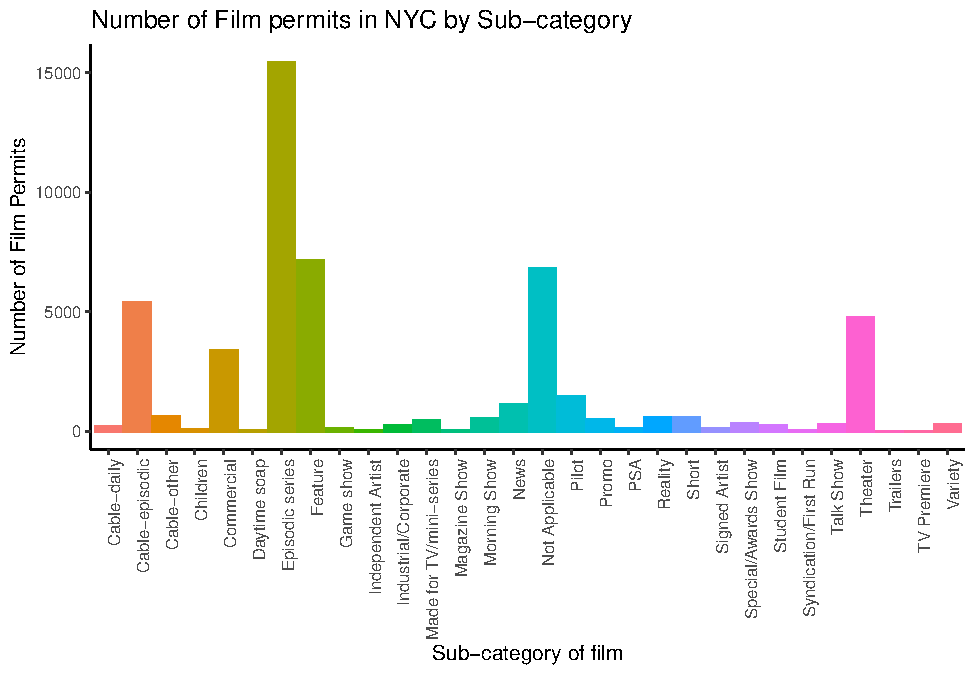
\includegraphics{Statistics_Lab_files/figure-latex/1subcategory-1.pdf}

I guess ``episodic series'' are the most common. Using a graph like this gave us our answer super fast.

\hypertarget{categories-by-different-boroughs}{%
\subsubsection{Categories by different Boroughs}\label{categories-by-different-boroughs}}

Let's see one more really useful thing about ggplot2. It's called \texttt{facet\_wrap()}. It's an ugly word, but you will see that it is very cool, and you can do next-level-super-hero graph styles with \texttt{facet\_wrap} that other people can't do very easily.

Here's our question. We know that some films are made in different Boroughs, and that same films are made in different categories, but do different Boroughs have different patterns for the kinds of categories of films they request permits for? Are their more TV shows in Brooklyn? How do we find out? Watch, just like this:

\begin{Shaded}
\begin{Highlighting}[]
\CommentTok{\# get the counts (this is a comment it\textquotesingle{}s just here for you to read)}

\NormalTok{counts }\OtherTok{\textless{}{-}}\NormalTok{ nyc\_films }\SpecialCharTok{\%\textgreater{}\%}
          \FunctionTok{group\_by}\NormalTok{(Borough,Category) }\SpecialCharTok{\%\textgreater{}\%}
          \FunctionTok{summarize}\NormalTok{(}\AttributeTok{count\_of\_permits =} \FunctionTok{length}\NormalTok{(Category))}

\CommentTok{\# make the plot}

\FunctionTok{ggplot}\NormalTok{(counts, }\FunctionTok{aes}\NormalTok{(}\AttributeTok{x =}\NormalTok{ Category, }\AttributeTok{y =}\NormalTok{ count\_of\_permits, }
                   \AttributeTok{color=}\NormalTok{Category, }
                   \AttributeTok{fill=}\NormalTok{ Category )) }\SpecialCharTok{+}
  \FunctionTok{geom\_bar}\NormalTok{(}\AttributeTok{stat=}\StringTok{"identity"}\NormalTok{) }\SpecialCharTok{+} 
  \FunctionTok{theme\_classic}\NormalTok{(}\AttributeTok{base\_size =} \DecValTok{10}\NormalTok{) }\SpecialCharTok{+}
  \FunctionTok{theme}\NormalTok{(}\AttributeTok{axis.text.x =} \FunctionTok{element\_text}\NormalTok{(}\AttributeTok{angle =} \DecValTok{90}\NormalTok{, }\AttributeTok{hjust =} \DecValTok{1}\NormalTok{)) }\SpecialCharTok{+}
  \FunctionTok{ylab}\NormalTok{(}\StringTok{"Number of Film Permits"}\NormalTok{) }\SpecialCharTok{+} 
  \FunctionTok{xlab}\NormalTok{(}\StringTok{"Category of film"}\NormalTok{) }\SpecialCharTok{+}
  \FunctionTok{ggtitle}\NormalTok{(}\StringTok{"Number of Film permits in NYC by Category and Borough"}\NormalTok{) }\SpecialCharTok{+}
  \FunctionTok{theme}\NormalTok{(}\AttributeTok{legend.position=}\StringTok{"none"}\NormalTok{) }\SpecialCharTok{+}
  \FunctionTok{facet\_wrap}\NormalTok{(}\SpecialCharTok{\textasciitilde{}}\NormalTok{Borough, }\AttributeTok{ncol=}\DecValTok{3}\NormalTok{)}
\end{Highlighting}
\end{Shaded}

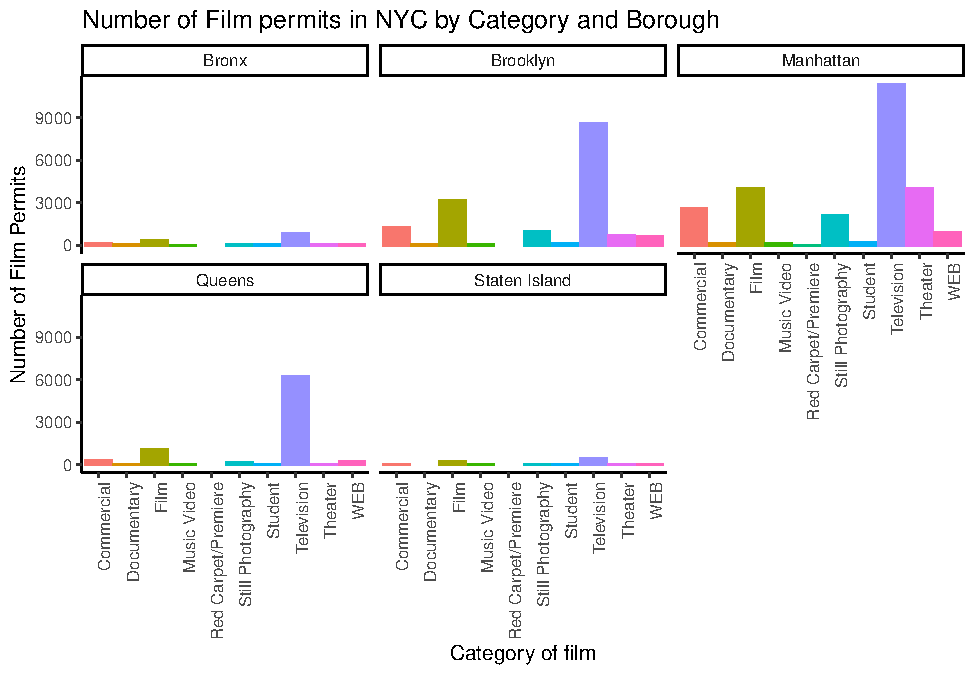
\includegraphics{Statistics_Lab_files/figure-latex/1facetwrap-1.pdf}

We did two important things. First we added \texttt{Borough} and \texttt{Category} into the \texttt{group\_by()} function. This automatically gives separate counts for each category of film, for each Borough. Then we added \texttt{facet\_wrap(\textasciitilde{}Borough,\ ncol=3)} to the end of the plot, and it automatically drew us 5 different bar graphs, one for each Borough! That was fast. Imagine doing that by hand.

The nice thing about this is we can switch things around if we want. For example, we could do it this way by switching the \texttt{Category} with \texttt{Borough}, and facet-wrapping by Category instead of Borough like we did above. Do what works for you.

\begin{Shaded}
\begin{Highlighting}[]
\FunctionTok{ggplot}\NormalTok{(counts, }\FunctionTok{aes}\NormalTok{(}\AttributeTok{x =}\NormalTok{ Borough, }\AttributeTok{y =}\NormalTok{ count\_of\_permits, }
                   \AttributeTok{color=}\NormalTok{Borough, }
                   \AttributeTok{fill=}\NormalTok{ Borough )) }\SpecialCharTok{+}
  \FunctionTok{geom\_bar}\NormalTok{(}\AttributeTok{stat=}\StringTok{"identity"}\NormalTok{) }\SpecialCharTok{+} 
  \FunctionTok{theme\_classic}\NormalTok{(}\AttributeTok{base\_size =} \DecValTok{10}\NormalTok{) }\SpecialCharTok{+}
  \FunctionTok{theme}\NormalTok{(}\AttributeTok{axis.text.x =} \FunctionTok{element\_text}\NormalTok{(}\AttributeTok{angle =} \DecValTok{90}\NormalTok{, }\AttributeTok{hjust =} \DecValTok{1}\NormalTok{)) }\SpecialCharTok{+}
  \FunctionTok{ylab}\NormalTok{(}\StringTok{"Number of Film Permits"}\NormalTok{) }\SpecialCharTok{+} 
  \FunctionTok{xlab}\NormalTok{(}\StringTok{"Borough"}\NormalTok{) }\SpecialCharTok{+}
  \FunctionTok{ggtitle}\NormalTok{(}\StringTok{"Number of Film permits in NYC by Category and Borough"}\NormalTok{) }\SpecialCharTok{+}
  \FunctionTok{theme}\NormalTok{(}\AttributeTok{legend.position=}\StringTok{"none"}\NormalTok{) }\SpecialCharTok{+}
  \FunctionTok{facet\_wrap}\NormalTok{(}\SpecialCharTok{\textasciitilde{}}\NormalTok{Category, }\AttributeTok{ncol=}\DecValTok{5}\NormalTok{)}
\end{Highlighting}
\end{Shaded}

\includegraphics{Statistics_Lab_files/figure-latex/1facetwrap2-1.pdf}

\hypertarget{gapminder-data}{%
\subsection{Gapminder Data}\label{gapminder-data}}

\url{https://www.gapminder.org} is an organization that collects some really interesting worldwide data. They also make cool visualization tools for looking at the data. There are many neat examples, and they have visualization tools built right into their website that you can play around with \url{https://www.gapminder.org/tools/}. That's fun check it out.

There is also an R package called \texttt{gapminder}. When you install this package, it loads in some of the data from gapminder, so we can play with it in R.

If you don't have the gapminder package installed, you can install it by running this code

\begin{Shaded}
\begin{Highlighting}[]
\FunctionTok{install.packages}\NormalTok{(}\StringTok{"gapminder"}\NormalTok{)}
\end{Highlighting}
\end{Shaded}

Once the package is installed, you need to load the new library, like this. Then, you can put the \texttt{gapminder} data into a data frame, like we do here: \texttt{gapminder\_df}.

\begin{Shaded}
\begin{Highlighting}[]
\FunctionTok{library}\NormalTok{(gapminder)}
\NormalTok{gapminder\_df}\OtherTok{\textless{}{-}}\NormalTok{gapminder}
\end{Highlighting}
\end{Shaded}

\hypertarget{look-at-the-data-frame}{%
\subsubsection{Look at the data frame}\label{look-at-the-data-frame}}

You can look at the data frame to see what is in it, and you can use \texttt{summarytools} again to view a summary of the data.

\begin{Shaded}
\begin{Highlighting}[]
\FunctionTok{view}\NormalTok{(}\FunctionTok{dfSummary}\NormalTok{(gapminder\_df))}
\end{Highlighting}
\end{Shaded}

There are 1704 rows of data, and we see some columns for country, continent, year, life expectancy, population, and GDP per capita.

\hypertarget{asking-questions-with-the-gap-minder-data}{%
\subsection{Asking Questions with the gap minder data}\label{asking-questions-with-the-gap-minder-data}}

We will show you how to graph some the data to answer a few different kinds of questions. Then you will form your own questions, and see if you can answer them with ggplot2 yourself. All you will need to do is copy and paste the following examples, and change them up a little bit

\hypertarget{life-expectancy-histogram}{%
\subsubsection{Life Expectancy histogram}\label{life-expectancy-histogram}}

How long are people living all around the world according to this data set? There are many ways we could plot the data to find out. The first way is a histogram. We have many numbers for life expectancy in the column \texttt{lifeExp}. This is a big sample, full of numbers for 142 countries across many years. It's easy to make a histogram in ggplot to view the distribution:

\begin{Shaded}
\begin{Highlighting}[]
\FunctionTok{ggplot}\NormalTok{(gapminder\_df, }\FunctionTok{aes}\NormalTok{(}\AttributeTok{x=}\NormalTok{lifeExp))}\SpecialCharTok{+}
  \FunctionTok{geom\_histogram}\NormalTok{(}\AttributeTok{color=}\StringTok{"white"}\NormalTok{)}
\end{Highlighting}
\end{Shaded}

\includegraphics{Statistics_Lab_files/figure-latex/1gapminder-1.pdf}

See, that was easy. Next, is a code block that adds more layers and settings if you wanted to modify parts of the graph:

\begin{Shaded}
\begin{Highlighting}[]
\FunctionTok{ggplot}\NormalTok{(gapminder\_df, }\FunctionTok{aes}\NormalTok{(}\AttributeTok{x =}\NormalTok{ lifeExp)) }\SpecialCharTok{+}
  \FunctionTok{geom\_histogram}\NormalTok{(}\AttributeTok{color=}\StringTok{"white"}\NormalTok{)}\SpecialCharTok{+} 
  \FunctionTok{theme\_classic}\NormalTok{(}\AttributeTok{base\_size =} \DecValTok{15}\NormalTok{) }\SpecialCharTok{+}
  \FunctionTok{ylab}\NormalTok{(}\StringTok{"Frequency count"}\NormalTok{) }\SpecialCharTok{+} 
  \FunctionTok{xlab}\NormalTok{(}\StringTok{"Life Expectancy"}\NormalTok{) }\SpecialCharTok{+}
  \FunctionTok{ggtitle}\NormalTok{(}\StringTok{"Histogram of Life Expectancy from Gapminder"}\NormalTok{)}
\end{Highlighting}
\end{Shaded}

\includegraphics{Statistics_Lab_files/figure-latex/1gapminderB-1.pdf}

The histogram shows a wide range of life expectancies, from below 40 to just over 80. Histograms are useful, they can show you what kinds of values happen more often than others.

One final thing about histograms in ggplot. You may want to change the bin size. That controls how wide or narrow, or the number of bars (how they split across the range), in the histogram. You need to set the \texttt{bins=} option in \texttt{geom\_histogram()}.

\begin{Shaded}
\begin{Highlighting}[]
\FunctionTok{ggplot}\NormalTok{(gapminder\_df, }\FunctionTok{aes}\NormalTok{(}\AttributeTok{x =}\NormalTok{ lifeExp)) }\SpecialCharTok{+}
  \FunctionTok{geom\_histogram}\NormalTok{(}\AttributeTok{color=}\StringTok{"white"}\NormalTok{, }\AttributeTok{bins=}\DecValTok{50}\NormalTok{)}\SpecialCharTok{+} 
  \FunctionTok{theme\_classic}\NormalTok{(}\AttributeTok{base\_size =} \DecValTok{15}\NormalTok{) }\SpecialCharTok{+}
  \FunctionTok{ylab}\NormalTok{(}\StringTok{"Frequency count"}\NormalTok{) }\SpecialCharTok{+} 
  \FunctionTok{xlab}\NormalTok{(}\StringTok{"Life Expectancy"}\NormalTok{) }\SpecialCharTok{+}
  \FunctionTok{ggtitle}\NormalTok{(}\StringTok{"Histogram of Life Expectancy from Gapminder"}\NormalTok{)}
\end{Highlighting}
\end{Shaded}

\includegraphics{Statistics_Lab_files/figure-latex/1gapminderC-1.pdf}

See, same basic patter, but now breaking up the range into 50 little equal sized bins, rather than 30, which is the default. You get to choose what you want to do.

\hypertarget{life-expectancy-by-year-scatterplot}{%
\subsubsection{Life Expectancy by year Scatterplot}\label{life-expectancy-by-year-scatterplot}}

We can see we have data for life expectancy and different years. So, does worldwide life expectancy change across the years in the data set? As we go into the future, are people living longer?

Let's look at this using a scatter plot. We can set the x-axis to be year, and the y-axis to be life expectancy. Then we can use \texttt{geom\_point()} to display a whole bunch of dots, and then look at them. Here's the simple code:

\begin{Shaded}
\begin{Highlighting}[]
\FunctionTok{ggplot}\NormalTok{(gapminder\_df, }\FunctionTok{aes}\NormalTok{(}\AttributeTok{y=}\NormalTok{ lifeExp, }\AttributeTok{x=}\NormalTok{ year))}\SpecialCharTok{+}
  \FunctionTok{geom\_point}\NormalTok{()}
\end{Highlighting}
\end{Shaded}

\includegraphics{Statistics_Lab_files/figure-latex/1scatterplot-1.pdf}

Whoa, that's a lot of dots! Remember that each country is measured each year. So, the bands of dots you see, show the life expectancies for the whole range of countries within each year of the database. There is a big spread inside each year. But, on the whole it looks like groups of dots slowly go up over years.

\hypertarget{one-country-life-expectancy-by-year}{%
\subsubsection{One country, life expectancy by year}\label{one-country-life-expectancy-by-year}}

I'm (Matt) from Canada, so maybe I want to know if life expectancy for Canadians is going up over the years. To find out the answer for one country, we first need to split the full data set, into another smaller data set that only contains data for Canada. In other words, we want only the rows where the word ``Canada'' is found in the \texttt{country} column. We will use the \texttt{filter} function from \texttt{dplyr} for this:

\begin{Shaded}
\begin{Highlighting}[]
\CommentTok{\# filter rows to contain Canada}

\NormalTok{smaller\_df }\OtherTok{\textless{}{-}}\NormalTok{ gapminder\_df }\SpecialCharTok{\%\textgreater{}\%} 
                 \FunctionTok{filter}\NormalTok{(country }\SpecialCharTok{==} \StringTok{"Canada"}\NormalTok{)}

\CommentTok{\# plot the new data contained in smaller\_df}

\FunctionTok{ggplot}\NormalTok{(smaller\_df, }\FunctionTok{aes}\NormalTok{(}\AttributeTok{y=}\NormalTok{ lifeExp, }\AttributeTok{x=}\NormalTok{ year))}\SpecialCharTok{+}
  \FunctionTok{geom\_point}\NormalTok{()}
\end{Highlighting}
\end{Shaded}

\includegraphics{Statistics_Lab_files/figure-latex/1scatterB-1.pdf}

I would say things are looking good for Canadians, their life expectancy is going up over the years!

\hypertarget{multiple-countries-scatterplot}{%
\subsubsection{Multiple countries scatterplot}\label{multiple-countries-scatterplot}}

What if we want to look at a few countries altogether. We can do this too. We just change how we filter the data so more than one country is allowed, then we plot the data. We will also add some nicer color options and make the plot look pretty. First, the simple code:

\begin{Shaded}
\begin{Highlighting}[]
\CommentTok{\# filter rows to contain countries of choice}

\NormalTok{smaller\_df }\OtherTok{\textless{}{-}}\NormalTok{ gapminder\_df }\SpecialCharTok{\%\textgreater{}\%} 
                 \FunctionTok{filter}\NormalTok{(country }\SpecialCharTok{\%in\%} \FunctionTok{c}\NormalTok{(}\StringTok{"Canada"}\NormalTok{,}\StringTok{"France"}\NormalTok{,}\StringTok{"Brazil"}\NormalTok{) }\SpecialCharTok{==} \ConstantTok{TRUE}\NormalTok{)}

\CommentTok{\# plot the new data contained in smaller\_df}

\FunctionTok{ggplot}\NormalTok{(smaller\_df, }\FunctionTok{aes}\NormalTok{(}\AttributeTok{y=}\NormalTok{ lifeExp, }\AttributeTok{x=}\NormalTok{ year, }\AttributeTok{group=}\NormalTok{ country))}\SpecialCharTok{+}
  \FunctionTok{geom\_point}\NormalTok{()}
\end{Highlighting}
\end{Shaded}

\includegraphics{Statistics_Lab_files/figure-latex/1scatterC-1.pdf}

Nice, we can now see three sets of dots, but which are countries do they represent? Let's add a legend, and make the graph better looking.

\begin{Shaded}
\begin{Highlighting}[]
\FunctionTok{ggplot}\NormalTok{(smaller\_df,}\FunctionTok{aes}\NormalTok{(}\AttributeTok{y=}\NormalTok{ lifeExp, }\AttributeTok{x=}\NormalTok{ year, }
                      \AttributeTok{group=}\NormalTok{ country, }\AttributeTok{color =}\NormalTok{ country)) }\SpecialCharTok{+}
  \FunctionTok{geom\_point}\NormalTok{()}\SpecialCharTok{+} 
  \FunctionTok{theme\_classic}\NormalTok{(}\AttributeTok{base\_size =} \DecValTok{15}\NormalTok{) }\SpecialCharTok{+}
  \FunctionTok{ylab}\NormalTok{(}\StringTok{"Life Expectancy"}\NormalTok{) }\SpecialCharTok{+} 
  \FunctionTok{xlab}\NormalTok{(}\StringTok{"Year"}\NormalTok{) }\SpecialCharTok{+}
  \FunctionTok{ggtitle}\NormalTok{(}\StringTok{"Life expectancy by year for three countries"}\NormalTok{)}
\end{Highlighting}
\end{Shaded}

\includegraphics{Statistics_Lab_files/figure-latex/1scatterD-1.pdf}

\hypertarget{geom_line-connecting-the-dots}{%
\subsubsection{geom\_line() connecting the dots}\label{geom_line-connecting-the-dots}}

We might also want to connect the dots with a line, to make it easier to see the connection! Remember, ggplot2 draws layers on top of layers. So, we add in a new \texttt{geom\_line()} layer.

\begin{Shaded}
\begin{Highlighting}[]
\FunctionTok{ggplot}\NormalTok{(smaller\_df,}\FunctionTok{aes}\NormalTok{(}\AttributeTok{y=}\NormalTok{ lifeExp, }\AttributeTok{x=}\NormalTok{ year, }
                      \AttributeTok{group=}\NormalTok{ country, }\AttributeTok{color =}\NormalTok{ country)) }\SpecialCharTok{+}
  \FunctionTok{geom\_point}\NormalTok{()}\SpecialCharTok{+} 
  \FunctionTok{geom\_line}\NormalTok{()}\SpecialCharTok{+}
  \FunctionTok{theme\_classic}\NormalTok{(}\AttributeTok{base\_size =} \DecValTok{15}\NormalTok{) }\SpecialCharTok{+}
  \FunctionTok{ylab}\NormalTok{(}\StringTok{"Life Expectancy"}\NormalTok{) }\SpecialCharTok{+} 
  \FunctionTok{xlab}\NormalTok{(}\StringTok{"Year"}\NormalTok{) }\SpecialCharTok{+}
  \FunctionTok{ggtitle}\NormalTok{(}\StringTok{"Life expectancy by year for three countries"}\NormalTok{)}
\end{Highlighting}
\end{Shaded}

\includegraphics{Statistics_Lab_files/figure-latex/1scatline-1.pdf}

\hypertarget{generalization-exercise}{%
\subsection{Generalization Exercise}\label{generalization-exercise}}

The following generalization exercise and writing assignment is also in your lab R Markdown document for this lab. Complete your work in that document and hand it in.

(1 point - Pass/Fail)

Use the code from above to attempt to solve the extra things we ask you do for this assignment. You generalization exercises are as follows:

\begin{enumerate}
\def\labelenumi{\arabic{enumi}.}
\item
  Make a graph plotting Life Expectancy by year for the five continents, using the \texttt{continent} factor. Make sure you change the title so it reads correctly
\item
  Make a graph plotting GDP per capita by year for the USA, Canada, and Mexico. Use the \texttt{gdpPercap} column for the GDP per capita data
\item
  Make a new graph plotting anything you are interested in using the gapminder dataset. It just needs to be a plot that we have not given an example for
\end{enumerate}

\hypertarget{writing-assignment}{%
\subsection{Writing assignment}\label{writing-assignment}}

Complete the writing assignment described in your R Markdown document for this lab. When you have finished everything. Knit the document and hand in your stuff (you can submit your .RMD file to blackboard if it does not knit.)

The question for this lab is a long answer question about histograms. Here is the question:

Describe what histograms are, how to interpret them, and what they are useful for. You should answer each of these questions:

The answers to each of these questions are worth .25 points each, for a total of 2 points

\begin{enumerate}
\def\labelenumi{\alph{enumi}.}
\tightlist
\item
  What do the bars on a histogram represent?
\item
  How many bars can a histogram have?
\item
  What do the heights of the bars tell you
\item
  What is on the x-axis and y-axis of a histogram
\item
  What does the tallest bar on a histogram tell you?
\item
  What does the shortest bar on a histogram tell you?
\item
  What are some uses for histograms, why would you want to look at a histogram of some numbers that you collected?
\item
  Imagine you had two histograms, one was very wide and spread out, the other was very narrow with a very tall peak. Which histogram would you expect to contain more consistent numbers (numbers that are close to each other), explain why.
\end{enumerate}

\textbf{Rubric}

General grading.

\begin{itemize}
\tightlist
\item
  You will receive 0 points for missing answers (say, if you do not answer question c, then you will receive 0 out .25 points for that question)
\item
  You must write in complete sentences. Point form sentences will be given 0 points.
\item
  Completely incorrect answers will receive 0 points. For example, if you incorrectly describe what the x and y-axes refer to, then you will receive 0 points for that question.
\item
  If your answer is generally correct but very difficult to understand and unclear you may receive half points for the question
\end{itemize}

\hypertarget{excel-1}{%
\section{Excel}\label{excel-1}}

\hypertarget{spss-1}{%
\section{SPSS}\label{spss-1}}

In this lab, we will get you acquainted with the SPSS software layout and graph some sample data to make sense of it. We will be doing the following:

\begin{enumerate}
\def\labelenumi{\arabic{enumi}.}
\tightlist
\item
  Opening SPSS and the SPSS layout
\item
  Reviewing variable properties and the Variable View tab
\item
  Opening a data file and producing different types of graphs
\end{enumerate}

\hypertarget{opening-spss-and-the-spss-layout-1}{%
\subsection{Opening SPSS and the SPSS layout}\label{opening-spss-and-the-spss-layout-1}}

Your lab instructor will take you through the process of opening the SPSS program. You may double-click on its icon located on the desktop of your lab computer, or you may find it using the Start menu. Once the program loads, you will be prompted with a pop-up window that asks you which file you would like to open. For now, we will be examining the basic layout of SPSS without a data set, so you can click {Cancel}.

Once you do, the main SPSS spreadsheet should open. It will look like this, a basic spreadsheet:

\begin{figure}
\centering
\includegraphics{img/1.4.11.png}
\caption{\label{fig:unnamed-chunk-42}Empty SPSS spreadsheet}
\end{figure}

Notice at the bottom of your window there are two tabs; ``Data View'' and ``Variable View''. In data view, we enter data into our spreadsheet. You will notice that rows are numbered on the left-hand side of the spreadsheet, while columns are labeled ``var''. This is an indication of the general structure of SPSS: Variables are contained in the columns, and rows indicate individual observations. For example, if you obtained the heights (in inches) of 5 people \{x= 64, 70, 63, 62, 65\} and wanted to enter their data into SPSS, each person's height would be entered in a new row, not across the columns, as seen below:

\includegraphics{img/1.4.12.png}

\hypertarget{reviewing-variable-properties-and-the-variable-view-tab-1}{%
\subsection{Reviewing variable properties and the Variable View tab}\label{reviewing-variable-properties-and-the-variable-view-tab-1}}

Now that we have some data entered, we might want to name our variable so that it's evident our measurements represent heights. In order to view or modify variable names and other properties, look to the bottom of your SPSS window and switch over to the ``Data View'' tab. Once you do this, your window will appear as follows:

\includegraphics{img/1.4.13.png}

Here, you can edit the name of your variables, and specify their properties. Variable names can be anything you like, with the restriction that you cannot use numbers or spaces. Next, notice several other important properties of variables you may at some point need to set or modify:

\begin{itemize}
\tightlist
\item
  Name: the name of your variable that will appear as a column header in Data View. No spaces or numerals.
\item
  Type: Your data will most often be Numeric, but sometimes, as in data representing currency or data in scientific notation, you may change the data type appropriately. If your data is simply a label, word, or response (such as an open-ended response to a survey question), choose ``String'': this tells SPSS not to treat this variable as a number. (Nota bene: if you select the wrong type of variable, SPSS may not be able to process your requested calculations, so always remember to check this parameter!)
\item
  Width: This refers to how many digits will be visible by default.
\item
  Decimals: This refers to how many decimal places will be visible by default.
\item
  Label: This is a description of the variable. Any information too long to be included in the variable name goes here.
\item
  Values: For nominal scale data, let's say 1 represents male and 2 represents female, this is where you include the values and their corresponding labels.
\item
  Measure: This variable property allows you to specify the nature of your data. Depending on the kind of scale you are using, you will choose a different measure type. Nominal and ordinal are chosen for nominal and ordinal scales, respectively. ``Scale'' is used when your data is measured on a ratio or interval scale.
\end{itemize}

\hypertarget{opening-a-data-file-and-producing-different-types-of-graphs}{%
\subsection{Opening a data file and producing different types of graphs}\label{opening-a-data-file-and-producing-different-types-of-graphs}}

Now that we know about the properties of the SPSS spreadsheet window, let's open a data file and learn how to make some sense of it by creating different types of graphs. Use the `nyc\_films.sav' file from the zip file you downloaded in section 0.2.3, which contains information about film permits (requests made by film companies to shoot TV shows and movies on location) filed in New York City.

Once you open the data file, browse through to familiarize yourself with the variables that are being measured. Switch over to Variable View for details of each variable.

\hypertarget{bar-graphs}{%
\subsubsection{Bar Graphs}\label{bar-graphs}}

Now, back to Data View. We will not be working with every single variable in this spreadsheet, but we'll select a few interesting ones with which to answer questions. Let's start with \texttt{borough}. Suppose we wanted to know which borough receives the most film permits (you can probably guess which one is most popular). Let's use SPSS to produce a graph to answer this question. With your data file open, go up to the top menu and choose {Graphs}, then {Legacy Dialogs}. You will see an entire list of possible graphs we can use to plot our data.

Let's think about the nature of our question: we would like to know how many permits were filed for each borough. Borough is simply a label or a name for a region, and we want to know the frequency of permits for each borough. This is a nominal scale variable and so, we will appropriately choose a BAR graph to plot it. Select {Bar\ldots{}}

\includegraphics{img/1.4.14.png}

The next window will ask you to specify what kind of graph you would like. Select {Simple} and then {Define}.
\includegraphics{img/1.4.15.png}
The following window will ask which variable you'd like to plot. Select \texttt{borough} from the left-hand list and use the arrow to move it into the field labeled ``Category Axis''. Then click {OK}.

\includegraphics{img/1.4.16.png}

SPSS will produce a new output window which will contain the bar graph you have generated. Notice which borough receives the most film permits. Note: your graph might be a different colour.

\includegraphics{img/1.4.17.png}

\hypertarget{histograms}{%
\subsubsection{Histograms}\label{histograms}}

Now, let's use a different data set to plot a histogram. The defining difference between a histogram and a bar graph (although they look very similar as they both utilize bars) is that a histogram is used to display a continuous variable (interval or ratio scale). In the previous example, boroughs were simply labels or names, so we used a nominal scale and therefore a bar graph. Here, we will deal with life expectancy (measured in years), an interval scale measure. Open life\_expectancy.sav (from the zip file you downloaded from 0.2.3). Open this file and examine its rows and columns. Each column represents a year during which life expectancy was measured. Each row represents a different country.

Let's first get an idea about life expectancy in general. We want to plot a histogram with life expectancy on the x-axis and frequency on the y-axis. Choose {Graphs} in the top menu, then {Legacy Dialogs}. From here, remember we want a histogram, not a bar graph, so let's select {Histogram\ldots{}}.

\includegraphics{img/1.4.18.png}

The window that appears contains every variable in your spreadsheet listed on the left-hand side. We can choose one variable at a time to plot. Let's scroll all the way down the list and choose \texttt{2017\ {[}v219{]}}. This is the variable containing life expectancies for the year 2017. Using the arrow, move that variable into the field labeled ``Variable:'', then click {OK}.

\includegraphics{img/1.4.19.png}

SPSS will produce an output window containing the distribution of life expectancy for the year 2017. Note: You may get different axis intervals/labels than what is shown here.

\includegraphics{img/1.4.20.png}

\hypertarget{scatterplots}{%
\subsubsection{Scatterplots}\label{scatterplots}}

Now, we will look to a different type of data plot; the scatterplot. A scatterplot allows us to visualize bivariate data, that is, data for which there are two measurements per individual. For example, we may ask whether life expectancy in a country (or how long you live, on average) is related to the average income. Using the life\_expectancy.sav data file, let's plot both variables: \texttt{2017\ {[}v219{]}} and \texttt{income}. The income variable in the spreadsheet refers to data collected in 2017 by the Better Life Initiative. Notice not all the countries listed have estimates for average annual income. For those that do, this value represents household net adjusted income (annual) in US dollars.

To create the scatterplot, let's go to {Graphs} in the menu toolbar, then {Legacy Dialogs}, then {Scatter}.

\includegraphics{img/1.4.21.png}

You will choose {Simple} scatter, then click {Define}.
\includegraphics{img/1.4.22.png}

Next, indicate which variables (there are 2 this time!) you would like in the x- and y-axes. Use the arrows to place \texttt{income} in the x-axis field, and \texttt{2017\ (V219)} in the y-axis field. (For the purposes of graphing a scatterplot, it does not matter which variable goes into the y-axis and x-axis fields for now; you can reverse them if you'd like and you can still interpret the data similarly)

\includegraphics{img/1.4.23.png}

Then click {OK}.
SPSS will produce output containing a scatterplot. What relationship do you notice? What happens to life expectancy the more individuals earn, on average?

\includegraphics{img/1.4.24.png}

\hypertarget{homework-1}{%
\subsection{Homework}\label{homework-1}}

\begin{center}\rule{0.5\linewidth}{0.5pt}\end{center}

Create the following three graphs in a single SPSS output file (*.spv). Upload this file to Moodle and use the graphs to answer the questions in the homework ``quiz'' on Moodle. Note that you can attempt the quiz as many times as you like before the due date and only your highest mark will be counted.

\begin{enumerate}
\def\labelenumi{\arabic{enumi}.}
\tightlist
\item
  Create a histogram for life expectancy in the year 1800.
\item
  If you haven't already, create a histogram for life expectancy in the year 2017.
\item
  Create a scatterplot of life expectancy of each country in 1800 vs.~that of 2018.
\end{enumerate}

\hypertarget{jamovi---week-4---january-30th-31st}{%
\section{JAMOVI - Week 4 - January 30th \& 31st}\label{jamovi---week-4---january-30th-31st}}

This section is copied almost verbatim, with some editorial changes, from \href{https://www.erinmazerolle.com/statisticsLab/lab-1-graphing-data.html\#spss-1}{Answering questions with data: The lab manual for R, Excel, SPSS and JAMOVI, Lab 1, Section 1.4, SPSS}, according to its \href{https://creativecommons.org/licenses/by-sa/4.0/deed.ast}{CC license}. Thank you to Crump, Krishnan, Volz, \& Chavarga (2018).

In this lab, it is hoped you will become more acquainted with the jamovi software layout and graph some sample data to make sense of it. We will be doing the following:

\begin{enumerate}
\def\labelenumi{\arabic{enumi}.}
\tightlist
\item
  Deciding on which is the best graph based on the scale of measurement
\item
  Reviewing variable attributes (or properties) using the Edit (in Variables menu) or Setup (in Data menu) buttons
\item
  Opening a data file and producing different types of graphs
\end{enumerate}

\hypertarget{opening-jamovi-and-reviewing-the-jamovi-layout}{%
\subsection{Opening JAMOVI and Reviewing the JAMOVI Layout}\label{opening-jamovi-and-reviewing-the-jamovi-layout}}

To open jamovi if you are using Windows, either double-click its icon located on the desktop of your computer, or click it in the Start menu.

To open jamovi if you are using a Mac, find the icon in your Applications folder and double-click it.

Once the program loads, you can click on the button that looks like three horizontal lines at the top left. This bottom reveals a menu. Take note that you have some familiar options here: {New} (for a new file), {Open} (to open an existing file), and {Save}. For now, we will be reviewing the basic layout of jamovi without a data set, so you can click the left facing arrow to close this menu.

Once you do, the main jamovi spreadsheet should be apparent. It will look like this, with a basic spreadsheet on the left and a results panel on the right:

\begin{figure}
\centering
\includegraphics{img/1.5.1.1.png}
\caption{\label{fig:unnamed-chunk-56}Empty jamovi spreadsheet}
\end{figure}

As explained in \href{https://www.erinmazerolle.com/statisticsLab/software.html\#getting-started-with-jamovi}{Section 0.6.1.2}, you can slide the separating line between these two panels to make one panel or the other larger. You should also recall that, in the spreadsheet, each row represents a case or a \emph{participant} and each column represents a \emph{variable}. (For more details about the jamovi program, see Section 0.6.) If, for example, you obtained the heights (in inches) of 5 people \{x = 64, 70, 63, 62, 65\} and wanted to enter their data into jamovi, each person's height would be entered in a new row, as seen below, not across the columns:

\includegraphics{img/1.5.1.2.png}

\hypertarget{reviewing-variable-properties-and-the-edit-or-setup-button}{%
\subsection{Reviewing Variable Properties and the Edit or Setup button}\label{reviewing-variable-properties-and-the-edit-or-setup-button}}

Now that we have some data entered, we might want to name our variable so that it's evident our measurements represent heights. In order to view or modify variable names and other properties, look to the menu ribbon at the top of the jamovi window. Notice that when you are enterring data, you are working in the {Data} tab or menu (look at the top set of menu options). While you are within any column representing a variable, you can click the {Setup} button. This {Setup} button will reveal, in a top panel, information about the attributes of the variable. (You may recall from lab that the other way to access this panel is to have the variable name highlighted while in the {Variables}) menu and to click the {Edit} button.)

\includegraphics{img/1.5.2.1A.png}

Once selected, your window will appear as follows:

\includegraphics{img/1.5.2.1B.png}

A more detailed description of variable types is presented in \href{https://www.erinmazerolle.com/statisticsLab/software.html\#the-spreadsheet}{Section 0.6.3}. Within this variable panel, you can edit the name of your variables and specify their properties. Variable names can be anything you like (\emph{without the restrictions that SPSS has}). Based on some user feedback, however, you may want to consider using Camel Case or underscores in variable names to play it safe (ex. ParticipantNumber or Participant\_Number). Also, you may want to consider how much of the variable name you will see in the spreadsheet panel based on the size of screen and the number of variables you have in your data set.

\includegraphics{img/1.5.2.2A.png}

\includegraphics{img/1.5.2.2B.png}

Below the variable name is a place for a description of the data. Below the description is a drop-down menu allowing you to identify the measure type: nominal, ordinal, continuous, or ID. Below that is a drop-down menu allowing you to identify the data type: Integer, Decimal, or Text. The final variable attribute on the left side is a place for you to identify any missing values. To the left of the measure type, data type, and missing values is a box wherein levels can be specified. If you need to code data, this is the place to do so. (Just in case it helps you to know this: It is similar to the Values column in the Variable View of SPSS.) Selecting the ``Retain unused levels'' radio button forces the program to keep levels even if they do not appear in the data set.

\includegraphics{img/1.5.2.3.png}

You may want to click the arrowhead that points to the left or right to move to an adjacent variable. Alternatively, clicking the {Setup} button again or clicking the upward facing arrow will hide this variable attribute information from your view.

\hypertarget{opening-a-data-file-through-the-jamovi-software}{%
\subsection{Opening a Data File (Through the JAMOVI Software)}\label{opening-a-data-file-through-the-jamovi-software}}

Now that we know about the properties of the jamovi spreadsheet window, let's open a data file and learn how to make some sense of it by creating different types of graphs. (It is not important for you to {Save} the jamovi file you just created because we will not be doing anything with those fictitious height data).

For a previous lab, you agreed to some terms of use regarding the data set we will be using in this lab. Then, you downloaded the data file and saved the file somewhere sensible on your computer so you could find it later.

In jamovi, click the button that looks like three horizontal lines at the top left. Select {Open}. Click {Browse}, locate the jamovi file you downloaded (\emph{EngageNS\_StartingFile\_2023.omv}), and double click. It is a somewhat large file and will take a few minutes to import. Once it is finished, we want to save it in jamovi format (.omv) using a new name to indicate you will change it for the lab demonstration. Click the button that looks like three horizontal lines at the top left. Select {Save As}, type a sensible name for your file, ensure it is set to ``jamovi file (.omv)'', click browse and select the folder in which to save your file, and click {Save}. (Mac users may need to copy the file, paste it, and rename it.) Remember that EngageNS surveyed Nova Scotians about various aspects of their quality of life.

The data dictionary, which is a .pdf file (in this case), lists all the variables that were included in the EngageNS survey and shows how these variables were measured.You should open this file, too. (It is not a jamovi file, and you should be able to open it by double-clicking on the file name - \emph{CIW-NovaScotia2019-SurveyDataDictionary} - wherever you saved the file.)

Once you open the data file, browse through to familiarize yourself with the variables that are being measured. Take a look at the rows and columns in each file. Each \textbf{column} represents a \textbf{different variable} that was measured in the EngageNS survey. Each \textbf{row} represents the responses of a \textbf{single survey respondent}.

After opening the data file and data dictionary, browse through both files to familiarize yourself with the variables that are being measured. After you review the ``Variable label'' (second column) and the ``Response options'' (third column) in the data dictionary, switch over to Variable View in the data file to check the variable attributes of each variable.

Switch over to the {Variables} menu for a list of variables, and a quick view of the details of each variable (See the icon to the left of the variable name and the description to the right of the variable name). Sometimes this information is correct, but sometimes it is erroneous. We can use the data dictionary and what we know about scales of measurement to input the correct scales of measurement as needed.

The scale of measurement will help us consider the most appropriate type of graph for the data collected on any given variable.

\hypertarget{producing-different-types-of-graphs}{%
\subsection{Producing Different Types of Graphs}\label{producing-different-types-of-graphs}}

\hypertarget{bar-graphs-and-histograms}{%
\subsubsection{Bar Graphs and Histograms}\label{bar-graphs-and-histograms}}

Bar graphs and histograms are different types of graphs. Bar graphs are used for nominal variables. The \emph{y}-axis of a bar graph could be the mean of each level, the frequency of each level, or some other summary of each level.

Histograms are used for continuous variables (interval or ratio scales of measurement). The \emph{y}-axis is always frequency. Sometimes they are labeled ``count'' or ``density,'' but they always represent the number of times certain values appear in the data.

Are ordinal variables continuous? No.~However, many ordinal variables can be conceptualized as quasi-interval. Likert scales are often quasi-interval. For the scale to be quasi-interval, we generally require at least five options on the scale. In addition, it should be reasonable to assume equal spacing between options on the scale. For example, a scale with the following options might be considered quasi-interval, because there are five options and they all seem equally spaced from one another:
Strongly disagree, somewhat disagree, neither agree or disagree, somewhat agree, strongly agree

A quirk of JAMOVI is that histograms do not include numbers across all of the \emph{y}-axis, which makes them difficult to read. However, bar graphs do include numbers below each bar on the \emph{y}-axis in JAMOVI. For small, quasi-interval scales, you \textbf{could} (\emph{See note that follows this paragraph.}) approximate a histogram with a bar graph. The biggest difference is that usually histograms do not have any space between the bars, whereas bar graphs do have space between the bars, but this is not problematic for small, quasi-interval scales. (\textbf{Remember: In 292, for the 2024 Winter term, you will treat Likert scales that are quasi-interval with \emph{reasonably equal intervals} as interval scales. Therefore, you will use histograms when graphing these quasi-interval scales.})

\hypertarget{bar-graphs-1}{%
\subsubsection{Bar Graphs}\label{bar-graphs-1}}

Now, let's have a look at the spreadsheet showing the data set using the {Data} menu. We will not be working with every single variable in this spreadsheet, but we'll select a few interesting ones with which to answer questions. Let's start with \texttt{PARSPORT}. Suppose we want to know how many respondents in the EngageNS survey are members of or participants in sports or recreational organizations. Let's use JAMOVI to produce a graph to answer the question. Go up to the top menu and choose {Analyses}, then select {Exploration}, and then select {Descriptives}.

Let's think about the nature of our question. We want to know how many people in the data set indicated that they participate in sports and/or recreational organizations. From a quick check in the data dictionary, we can determine that \texttt{PARSPORT} is the name of the variable, it represents whether the survey respondent is a member or participant in sports or recreational activities, and it is measured using Yes/No response options. These response options represent a nominal scale, so we will appropriately choose a BAR graph to plot it. (Bar graphs are used to represent nominal scales because nominal scales are not continuous. In bar graphs, the bars do not touch -- showing the non-continuous nature of the scale.)

\includegraphics{img/PARSPORTinDataDictionary.png}

In the analysis panel (the view to the left in JAMOVI), select the variable of interest for the graph by highlighting \texttt{PARSPORT} and using the right-facing arrow to move it to that Variables field on the right.

\includegraphics{img/MovingPARSPORTToVarField.png}

Then, click on the {Plots} ribbon. You will see a number of options available. Select {Bar plot}\ldots{}

\includegraphics{img/PARSPORTBarGraphCommands.png}

In the Results panel, you will see a Descriptives table was produced when you selected the variable, and a bar graph was produced when you selected \texttt{Bar\ plot.} Notice how many respondents are involved in sports/recreational organizations and how many are not. Roughly how many people participate in sports/recreational organizations? How many do not?

\includegraphics{img/PARSPORTBarGraph.png}

Your bar graph will have as many bars as there are categories in your nominal variable. For example, if you want to know how many respondents were from each region of NS, create a bar graph for REGION. The number of regions from which the survey participants come is represented by the number of bars on your graph. If you want to construct this graph without moving both \texttt{PARSPORT} and \texttt{REGION} into the same Descriptives table, you can click on the arrow that faces to the right to close the Descriptives analysis and bar plot that you just completed.

\includegraphics{img/PARSPORTBarGraphCommitToResults.png}

Then, click on the {Exploration} and {Descriptives} commands again. Now, you can repeat the process looking at only \texttt{REGION}. From how many regions in Canada did the survey participants come? (Yes, the labelling of the \emph{x}-axis is very difficult to read with the words overlapping.)

\includegraphics{img/REGIONBarGraph_MessyXAxis.png}

\hypertarget{histograms-1}{%
\subsubsection{Histograms}\label{histograms-1}}

Now, let's use a different variable to plot a histogram. The defining difference between a histogram and a bar graph (although they look very similar as they both utilize bars) is that a histogram is used to display a continuous variable (interval or ratio scale). A second difference, and one that is more noticeable, is that, in histograms, the bars touch one another while there are gaps between the bars in bar graphs. This is a visual way to show that these types of graphs represent variables measured on different scales of measurement. Histograms are used to represent variables that are measured on continuous scales (e.g., interval or ratio scales). The bars in a histogram touch indicating the continuous nature of the measurement scale. In the previous example, respondents indicated simply whether they were or were not participants in sports/recreational organizations. Their responses were either yes or no; therefore, the data is categorical and was measured on a nominal scale. Given that the data is categorical, the gaps between the bars in the bar graph we made earlier represent the non-continuous nature of the data.
Here, we will deal with people's self-reported mental health, \texttt{MNTLHLTH}. In the EngageNS survey, respondents were asked to rate their own mental health on a 5-point scale, ranging from 1 to 5 where 1 = poor, 2 = fair, 3 = good, 4 = very good, and 5 = excellent.
\textbf{This is a good example of a real data set where there is inaccurate information in the file you have been given.} Having looked at the data dictionary and viewed the response options, you would consider \texttt{MNTLHLTH} to have a quasi-interval scale; however, in JAMOVI we see the variable attributes indicating \texttt{MNTLHLTH} has a nominal scale (under Measure type). Depending on where you land on the quasi-interval scale controversy, you should change the ``Measure type'' to ordinal or continuous.

\includegraphics{img/MNTLHLTHWrongScale.png}

Let's plot a histogram for this variable. (Remember to close the Descriptives menu, by clicking on the arrow facing to the right, before you keep going unless you want to run the same analyses on a number of variables.) We want to put our variable of interest - mental health - on the \emph{x}-axis and frequency for each score on the \emph{y}-axis. If you will recall, there were a number of options for types of graphs in the sub-menu we used for the bar graph. It is in that sub-menu where we will find the histogram option.
Under the {Analyses} tab, choose {Exploration} and {Descriptives}. Let's either use the search function or scroll through the variable list to find \texttt{MNTLHLTH}. Using the arrow or dragging the highlighted variable and dropping it, move \texttt{MNTLHLTH} into the Variables field. Now, click on the {Plots} ribbon. From here, remember we want a histogram, not a bar graph, so let's select {Histogram}\ldots{}

\includegraphics{img/MNTLHLTHCommands.png}

JAMOVI will produce, in the Results panel, the distribution of scores for respondents' self-reported mental health. (Remember to save your file -- using a different name than that you use for your starting file -- if you think you may want to look at it again in the future.)

\includegraphics{img/MNTLHLTHHistogram.png}

\hypertarget{tables}{%
\subsection{Tables}\label{tables}}

Please see the lab Moodle site for a handout of what you are expected to know about APA-formatted tables.

\hypertarget{homework-2}{%
\subsection{Homework}\label{homework-2}}

See Moodle.

\hypertarget{thinking-about-data---practice-questions}{%
\subsection{Thinking about Data - Practice Questions}\label{thinking-about-data---practice-questions}}

\begin{enumerate}
\def\labelenumi{\arabic{enumi}.}
\tightlist
\item
  Describe what histograms are, how to interpret them, and what they are useful for. You should answer each of these questions:
\end{enumerate}

The answers to each of these questions are worth .25 points each, for a total of 2 points.

\begin{itemize}
\tightlist
\item
  What do the bars on a histogram represent?
\item
  How many bars can a histogram have?
\item
  What do the heights of the bars tell you?
\item
  What is on the \emph{x}-axis and \emph{y}-axis of a histogram?
\item
  What does the tallest bar on a histogram tell you?
\item
  What does the shortest bar on a histogram tell you?
\item
  What are some uses for histograms, or why would you want to look at a histogram of some numbers that you collected?
\item
  Imagine you had two histograms, one was very wide and spread out while the other was very narrow with a very tall peak. Which histogram would you expect to contain more consistent numbers (numbers that are close to each other)? Explain why.
\end{itemize}

Rubric
General grading.

You will receive 0 points for missing answers (say, if you do not answer question c, then you will receive 0 out .25 points for that question)

You must write in complete sentences. Point form sentences will be given 0 points.

Completely incorrect answers will receive 0 points. For example, if you incorrectly describe what the x and y-axes refer to, then you will receive 0 points for that question.

If your answer is generally correct but very difficult to understand and unclear, you may receive half points for the question.

\begin{enumerate}
\def\labelenumi{\arabic{enumi}.}
\setcounter{enumi}{1}
\item
  Create the appropriate graph for the HB\_SUBUSE variable. In this variable, respondents were asked ``In the past week, I engaged in substance use (e.g., recreational drugs).'' Responses were measured on a 7-point scale where 1 = very strongly disagree to 7 = very strongly agree, with 4 = neutral. What do you learn by looking at the graph?
\item
  Create the appropriate graph for GAMBLING. In this variable, respondents were asked ``In the past year, how often did you engage in gambling (e.g., video lottery; lottery tickets)? Responses were measured on the following scale: 1 = never, 2 = once in the past year, 3 = at least once every 6 months, 4 = at least once every 3 months, 5 = at least once a month, 6 = at least once a week. What do you learn by looking at the graph?
\item
  Use the data dictionary to find a variable you are interested in. Create the appropriate graph. What do you learn by looking at the graph?
\end{enumerate}

\hypertarget{lab-2-descriptive-statistics-and-more-graphs}{%
\chapter{Lab 2: Descriptive Statistics (and more graphs)}\label{lab-2-descriptive-statistics-and-more-graphs}}

{
Describing comic sensibility is near impossible. It's sort of an abstract silliness, that sometimes the joke isn't the star.
-Dana Carvey
}

The purpose of this lab is to show you how to compute basic descriptive statistics, including measures of central tendency (mean, mode, median) and variation (range, variance, standard deviation).

\hypertarget{general-goals-1}{%
\section{General Goals}\label{general-goals-1}}

\begin{enumerate}
\def\labelenumi{\arabic{enumi}.}
\tightlist
\item
  Compute measures of central tendency using software
\item
  Compute measures of variation using software
\item
  Ask some questions of a data set using descriptive statistics
\end{enumerate}

\hypertarget{important-info-1}{%
\subsection{Important info}\label{important-info-1}}

We will be using data from the gapminder project. You can download a small snippet of the data in .csv format from this link (note this dataset was copied from the gapminder library for R) gapminder.csv. If you are using R, then you can install the gapminder package. This method is described later in the R section.

\hypertarget{r-2}{%
\section{R}\label{r-2}}

\hypertarget{descriptives-basics-in-r}{%
\subsection{Descriptives basics in R}\label{descriptives-basics-in-r}}

We learned in lecture and from the textbook that data we want to use ask and answer questions often comes with loads of numbers. Too many numbers to look at all at once. That's one reason we use descriptive statistics. To reduce the big set of numbers to one or two summary numbers that tell use something about all of the numbers. R can produce descriptive statistics for you in many ways. There are base functions for most of the ones that you want. We'll go over some R basics for descriptive statistics, and then use our new found skills to ask some questions about real data.

\hypertarget{making-numbers-in-r}{%
\subsubsection{Making numbers in R}\label{making-numbers-in-r}}

In order to do descriptive statistics we need to put some numbers in a variable. You can also do this using the \texttt{c()} command, which stands for combine

\begin{Shaded}
\begin{Highlighting}[]
\NormalTok{my\_numbers }\OtherTok{\textless{}{-}} \FunctionTok{c}\NormalTok{(}\DecValTok{1}\NormalTok{,}\DecValTok{2}\NormalTok{,}\DecValTok{3}\NormalTok{,}\DecValTok{4}\NormalTok{)}
\end{Highlighting}
\end{Shaded}

There a few other handy ways to make numbers. We can use \texttt{seq()} to make a sequence. Here's making the numbers from 1 to 100

\begin{Shaded}
\begin{Highlighting}[]
\NormalTok{one\_to\_one\_hundred }\OtherTok{\textless{}{-}} \FunctionTok{seq}\NormalTok{(}\DecValTok{1}\NormalTok{,}\DecValTok{100}\NormalTok{,}\DecValTok{1}\NormalTok{)}
\end{Highlighting}
\end{Shaded}

We can repeat things, using rep. Here's making 10 5s, and 25 1s:

\begin{Shaded}
\begin{Highlighting}[]
\FunctionTok{rep}\NormalTok{(}\DecValTok{10}\NormalTok{,}\DecValTok{5}\NormalTok{)}
\end{Highlighting}
\end{Shaded}

\begin{verbatim}
## [1] 10 10 10 10 10
\end{verbatim}

\begin{Shaded}
\begin{Highlighting}[]
\FunctionTok{rep}\NormalTok{(}\DecValTok{1}\NormalTok{,}\DecValTok{25}\NormalTok{)}
\end{Highlighting}
\end{Shaded}

\begin{verbatim}
##  [1] 1 1 1 1 1 1 1 1 1 1 1 1 1 1 1 1 1 1 1 1 1 1 1 1 1
\end{verbatim}

\begin{Shaded}
\begin{Highlighting}[]
\NormalTok{all\_together\_now }\OtherTok{\textless{}{-}} \FunctionTok{c}\NormalTok{(}\FunctionTok{rep}\NormalTok{(}\DecValTok{10}\NormalTok{,}\DecValTok{5}\NormalTok{),}\FunctionTok{rep}\NormalTok{(}\DecValTok{1}\NormalTok{,}\DecValTok{25}\NormalTok{)) }
\end{Highlighting}
\end{Shaded}

\hypertarget{sum}{%
\subsubsection{Sum}\label{sum}}

Let's play with the number 1 to 100. First, let's use the \texttt{sum()} function to add them up

\begin{Shaded}
\begin{Highlighting}[]
\NormalTok{one\_to\_one\_hundred }\OtherTok{\textless{}{-}} \FunctionTok{seq}\NormalTok{(}\DecValTok{1}\NormalTok{,}\DecValTok{100}\NormalTok{,}\DecValTok{1}\NormalTok{)}
\FunctionTok{sum}\NormalTok{(one\_to\_one\_hundred)}
\end{Highlighting}
\end{Shaded}

\begin{verbatim}
## [1] 5050
\end{verbatim}

\hypertarget{length}{%
\subsubsection{Length}\label{length}}

We put 100 numbers into the variable \texttt{one\_to\_one\_hundred}. We know how many numbers there are in there. How can we get R to tell us? We use \texttt{length()} for that.

\begin{Shaded}
\begin{Highlighting}[]
\FunctionTok{length}\NormalTok{(one\_to\_one\_hundred)}
\end{Highlighting}
\end{Shaded}

\begin{verbatim}
## [1] 100
\end{verbatim}

\hypertarget{central-tendency}{%
\subsection{Central Tendency}\label{central-tendency}}

\hypertarget{mean}{%
\subsubsection{Mean}\label{mean}}

Remember the mean of some numbers is their sum, divided by the number of numbers. We can compute the mean like this:

\begin{Shaded}
\begin{Highlighting}[]
\FunctionTok{sum}\NormalTok{(one\_to\_one\_hundred)}\SpecialCharTok{/}\FunctionTok{length}\NormalTok{(one\_to\_one\_hundred)}
\end{Highlighting}
\end{Shaded}

\begin{verbatim}
## [1] 50.5
\end{verbatim}

Or, we could just use the \texttt{mean()} function like this:

\begin{Shaded}
\begin{Highlighting}[]
\FunctionTok{mean}\NormalTok{(one\_to\_one\_hundred)}
\end{Highlighting}
\end{Shaded}

\begin{verbatim}
## [1] 50.5
\end{verbatim}

\hypertarget{median}{%
\subsubsection{Median}\label{median}}

The median is the number in the exact middle of the numbers ordered from smallest to largest. If there are an even number of numbers (no number in the middle), then we take the number in between the two (decimal .5). Use the \texttt{median} function. There's only 3 numbers here. The middle one is 2, that should be the median

\begin{Shaded}
\begin{Highlighting}[]
\FunctionTok{median}\NormalTok{(}\FunctionTok{c}\NormalTok{(}\DecValTok{1}\NormalTok{,}\DecValTok{2}\NormalTok{,}\DecValTok{3}\NormalTok{))}
\end{Highlighting}
\end{Shaded}

\begin{verbatim}
## [1] 2
\end{verbatim}

\hypertarget{mode}{%
\subsubsection{Mode}\label{mode}}

R does not a base function for the Mode. You would have to write one for yourself. Here is an example of writing your own mode function, and then using it. Note I searched how to do this on Google, and am using the mode defined by \href{https://stackoverflow.com/questions/2547402/is-there-a-built-in-function-for-finding-the-mode}{this answer on stack overflow}

Remember, the mode is the most frequently occurring number in the set. Below 1 occurs the most, so the mode will be one.

\begin{Shaded}
\begin{Highlighting}[]
\NormalTok{my\_mode }\OtherTok{\textless{}{-}} \ControlFlowTok{function}\NormalTok{(x) \{}
\NormalTok{  ux }\OtherTok{\textless{}{-}} \FunctionTok{unique}\NormalTok{(x)}
\NormalTok{  ux[}\FunctionTok{which.max}\NormalTok{(}\FunctionTok{tabulate}\NormalTok{(}\FunctionTok{match}\NormalTok{(x, ux)))]}
\NormalTok{\}}

\FunctionTok{my\_mode}\NormalTok{(}\FunctionTok{c}\NormalTok{(}\DecValTok{1}\NormalTok{,}\DecValTok{1}\NormalTok{,}\DecValTok{1}\NormalTok{,}\DecValTok{1}\NormalTok{,}\DecValTok{1}\NormalTok{,}\DecValTok{1}\NormalTok{,}\DecValTok{1}\NormalTok{,}\DecValTok{2}\NormalTok{,}\DecValTok{3}\NormalTok{,}\DecValTok{4}\NormalTok{))}
\end{Highlighting}
\end{Shaded}

\begin{verbatim}
## [1] 1
\end{verbatim}

\hypertarget{variation}{%
\subsection{Variation}\label{variation}}

We often want to know how variable the numbers are. We are going to look at descriptive statistics to describe this such as the \textbf{range}, \textbf{variance}, the \textbf{standard deviation}, and a few others.

First, let's remind ourselves what variation looks like (it's when the numbers are different). We will sample 100 numbers from a normal distribution (don't worry about this yet), with a mean of 10, and a standard deviation of 5, and then make a histogram so we can see the variation around 10..

\begin{Shaded}
\begin{Highlighting}[]
\NormalTok{sample\_numbers }\OtherTok{\textless{}{-}} \FunctionTok{rnorm}\NormalTok{(}\DecValTok{100}\NormalTok{,}\DecValTok{10}\NormalTok{,}\DecValTok{5}\NormalTok{)}
\FunctionTok{hist}\NormalTok{(sample\_numbers)}
\end{Highlighting}
\end{Shaded}

\includegraphics{Statistics_Lab_files/figure-latex/unnamed-chunk-81-1.pdf}

\hypertarget{range}{%
\subsubsection{range}\label{range}}

The range is the minimum and maximum values in the set, we use the \texttt{range} function.

\begin{Shaded}
\begin{Highlighting}[]
\FunctionTok{range}\NormalTok{(sample\_numbers)}
\end{Highlighting}
\end{Shaded}

\begin{verbatim}
## [1] -3.814636 21.324221
\end{verbatim}

\hypertarget{var-variance}{%
\subsubsection{var = variance}\label{var-variance}}

We can find the sample variance using \texttt{var}. Note, divides by (n-1)

\begin{Shaded}
\begin{Highlighting}[]
\FunctionTok{var}\NormalTok{(sample\_numbers)}
\end{Highlighting}
\end{Shaded}

\begin{verbatim}
## [1] 20.35961
\end{verbatim}

\hypertarget{sd-standard-deviation}{%
\subsubsection{sd = standard deviation}\label{sd-standard-deviation}}

We find the sample standard deviation us SD. Note, divides by (n-1)

\begin{Shaded}
\begin{Highlighting}[]
\FunctionTok{sd}\NormalTok{(sample\_numbers)}
\end{Highlighting}
\end{Shaded}

\begin{verbatim}
## [1] 4.512163
\end{verbatim}

Remember that the standard deviation is just the square root of the variance, see:

\begin{Shaded}
\begin{Highlighting}[]
\FunctionTok{sqrt}\NormalTok{(}\FunctionTok{var}\NormalTok{(sample\_numbers))}
\end{Highlighting}
\end{Shaded}

\begin{verbatim}
## [1] 4.512163
\end{verbatim}

\hypertarget{all-descriptives}{%
\subsubsection{All Descriptives}\label{all-descriptives}}

Let's put all of the descriptives and other functions so far in one place:

\begin{Shaded}
\begin{Highlighting}[]
\NormalTok{sample\_numbers }\OtherTok{\textless{}{-}} \FunctionTok{rnorm}\NormalTok{(}\DecValTok{100}\NormalTok{,}\DecValTok{10}\NormalTok{,}\DecValTok{5}\NormalTok{)}

\FunctionTok{sum}\NormalTok{(sample\_numbers)}
\end{Highlighting}
\end{Shaded}

\begin{verbatim}
## [1] 960.5306
\end{verbatim}

\begin{Shaded}
\begin{Highlighting}[]
\FunctionTok{length}\NormalTok{(sample\_numbers)}
\end{Highlighting}
\end{Shaded}

\begin{verbatim}
## [1] 100
\end{verbatim}

\begin{Shaded}
\begin{Highlighting}[]
\FunctionTok{mean}\NormalTok{(sample\_numbers)}
\end{Highlighting}
\end{Shaded}

\begin{verbatim}
## [1] 9.605306
\end{verbatim}

\begin{Shaded}
\begin{Highlighting}[]
\FunctionTok{median}\NormalTok{(sample\_numbers)}
\end{Highlighting}
\end{Shaded}

\begin{verbatim}
## [1] 8.945858
\end{verbatim}

\begin{Shaded}
\begin{Highlighting}[]
\FunctionTok{my\_mode}\NormalTok{(sample\_numbers)}
\end{Highlighting}
\end{Shaded}

\begin{verbatim}
## [1] 2.222849
\end{verbatim}

\begin{Shaded}
\begin{Highlighting}[]
\FunctionTok{range}\NormalTok{(sample\_numbers)}
\end{Highlighting}
\end{Shaded}

\begin{verbatim}
## [1] -1.563686 21.926417
\end{verbatim}

\begin{Shaded}
\begin{Highlighting}[]
\FunctionTok{var}\NormalTok{(sample\_numbers)}
\end{Highlighting}
\end{Shaded}

\begin{verbatim}
## [1] 22.57911
\end{verbatim}

\begin{Shaded}
\begin{Highlighting}[]
\FunctionTok{sd}\NormalTok{(sample\_numbers)}
\end{Highlighting}
\end{Shaded}

\begin{verbatim}
## [1] 4.751748
\end{verbatim}

\hypertarget{descriptives-by-conditions}{%
\subsection{Descriptives by conditions}\label{descriptives-by-conditions}}

Sometimes you will have a single variable with some numbers, and you can use the above functions to find the descriptives for that variable. Other times (most often in this course), you will have a big data frame of numbers, with different numbers in different conditions. You will want to find descriptive statistics for each the sets of numbers inside each of the conditions. Fortunately, this is where R really shines, it does it all for you in one go.

Let's illustrate the problem. Here I make a date frame with 10 numbers in each condition. There are 10 conditions, each labelled, A, B, C, D, E, F, G, H, I, J.

\begin{Shaded}
\begin{Highlighting}[]
\NormalTok{scores }\OtherTok{\textless{}{-}} \FunctionTok{rnorm}\NormalTok{(}\DecValTok{100}\NormalTok{,}\DecValTok{10}\NormalTok{,}\DecValTok{5}\NormalTok{)}
\NormalTok{conditions }\OtherTok{\textless{}{-}} \FunctionTok{rep}\NormalTok{(}\FunctionTok{c}\NormalTok{(}\StringTok{"A"}\NormalTok{,}\StringTok{"B"}\NormalTok{,}\StringTok{"C"}\NormalTok{,}\StringTok{"D"}\NormalTok{,}\StringTok{"E"}\NormalTok{,}\StringTok{"F"}\NormalTok{,}\StringTok{"G"}\NormalTok{,}\StringTok{"H"}\NormalTok{,}\StringTok{"I"}\NormalTok{,}\StringTok{"J"}\NormalTok{), }\AttributeTok{each =}\DecValTok{10}\NormalTok{)}
\NormalTok{my\_df }\OtherTok{\textless{}{-}} \FunctionTok{data.frame}\NormalTok{(conditions,scores)}
\end{Highlighting}
\end{Shaded}

If you look at the \texttt{my\_df} data frame, you will see it has 100 rows, there are 10 rows for each condition with a label in the \texttt{conditions} column, and 10 scores for each condition in the \texttt{scores} column. What if you wanted to know the mean of the scores in each condition? You would want to find 10 means.

The slow way to do it would be like this:

\begin{Shaded}
\begin{Highlighting}[]
\FunctionTok{mean}\NormalTok{(my\_df[my\_df}\SpecialCharTok{$}\NormalTok{conditions}\SpecialCharTok{==}\StringTok{"A"}\NormalTok{,]}\SpecialCharTok{$}\NormalTok{scores)}
\end{Highlighting}
\end{Shaded}

\begin{verbatim}
## [1] 11.00857
\end{verbatim}

\begin{Shaded}
\begin{Highlighting}[]
\FunctionTok{mean}\NormalTok{(my\_df[my\_df}\SpecialCharTok{$}\NormalTok{conditions}\SpecialCharTok{==}\StringTok{"B"}\NormalTok{,]}\SpecialCharTok{$}\NormalTok{scores)}
\end{Highlighting}
\end{Shaded}

\begin{verbatim}
## [1] 13.68244
\end{verbatim}

\begin{Shaded}
\begin{Highlighting}[]
\FunctionTok{mean}\NormalTok{(my\_df[my\_df}\SpecialCharTok{$}\NormalTok{conditions}\SpecialCharTok{==}\StringTok{"C"}\NormalTok{,]}\SpecialCharTok{$}\NormalTok{scores)}
\end{Highlighting}
\end{Shaded}

\begin{verbatim}
## [1] 9.282638
\end{verbatim}

\begin{Shaded}
\begin{Highlighting}[]
\CommentTok{\# and then keep going}
\end{Highlighting}
\end{Shaded}

Nobody wants to do that! Not, me I stopped doing it that way, you should to.

\hypertarget{group_by-and-summarise}{%
\subsubsection{group\_by and summarise}\label{group_by-and-summarise}}

We can easily do everything all at once using the \texttt{group\_by} and \texttt{summarise} function from the \texttt{dplyr} package. Just watch

\begin{Shaded}
\begin{Highlighting}[]
\FunctionTok{library}\NormalTok{(dplyr)}

\NormalTok{my\_df }\SpecialCharTok{\%\textgreater{}\%}
  \FunctionTok{group\_by}\NormalTok{(conditions) }\SpecialCharTok{\%\textgreater{}\%}
  \FunctionTok{summarise}\NormalTok{(}\AttributeTok{means =} \FunctionTok{mean}\NormalTok{(scores))}
\end{Highlighting}
\end{Shaded}

\begin{verbatim}
## # A tibble: 10 x 2
##    conditions means
##    <chr>      <dbl>
##  1 A          11.0 
##  2 B          13.7 
##  3 C           9.28
##  4 D           8.65
##  5 E          12.4 
##  6 F           9.24
##  7 G           8.65
##  8 H           9.07
##  9 I           9.92
## 10 J          11.6
\end{verbatim}

A couple things now. First, the print out of this was ugly. Let's fix that. we put the results of our code into a new variable, then we use \texttt{knitr::kable} to print it out nicely when we \texttt{knit} the document

\begin{Shaded}
\begin{Highlighting}[]
\NormalTok{summary\_df }\OtherTok{\textless{}{-}}\NormalTok{ my\_df }\SpecialCharTok{\%\textgreater{}\%}
               \FunctionTok{group\_by}\NormalTok{(conditions) }\SpecialCharTok{\%\textgreater{}\%}
               \FunctionTok{summarise}\NormalTok{(}\AttributeTok{means =} \FunctionTok{mean}\NormalTok{(scores))}

\NormalTok{knitr}\SpecialCharTok{::}\FunctionTok{kable}\NormalTok{(summary\_df)}
\end{Highlighting}
\end{Shaded}

\begin{tabular}{l|r}
\hline
conditions & means\\
\hline
A & 11.008573\\
\hline
B & 13.682442\\
\hline
C & 9.282638\\
\hline
D & 8.651373\\
\hline
E & 12.387553\\
\hline
F & 9.243973\\
\hline
G & 8.647043\\
\hline
H & 9.067883\\
\hline
I & 9.922536\\
\hline
J & 11.638505\\
\hline
\end{tabular}

\hypertarget{multiple-descriptives}{%
\subsubsection{multiple descriptives}\label{multiple-descriptives}}

The best thing about the \texttt{dplyr} method, is that we can add more than one function, and we'll get more than one summary returned, all in a nice format, let's add the standard deviation:

\begin{Shaded}
\begin{Highlighting}[]
\NormalTok{summary\_df }\OtherTok{\textless{}{-}}\NormalTok{ my\_df }\SpecialCharTok{\%\textgreater{}\%}
               \FunctionTok{group\_by}\NormalTok{(conditions) }\SpecialCharTok{\%\textgreater{}\%}
               \FunctionTok{summarise}\NormalTok{(}\AttributeTok{means =} \FunctionTok{mean}\NormalTok{(scores),}
                         \AttributeTok{sds =} \FunctionTok{sd}\NormalTok{(scores))}

\NormalTok{knitr}\SpecialCharTok{::}\FunctionTok{kable}\NormalTok{(summary\_df)}
\end{Highlighting}
\end{Shaded}

\begin{tabular}{l|r|r}
\hline
conditions & means & sds\\
\hline
A & 11.008573 & 3.600200\\
\hline
B & 13.682442 & 4.863821\\
\hline
C & 9.282638 & 4.840763\\
\hline
D & 8.651373 & 4.326686\\
\hline
E & 12.387553 & 3.492181\\
\hline
F & 9.243973 & 4.281632\\
\hline
G & 8.647043 & 3.519232\\
\hline
H & 9.067883 & 3.456236\\
\hline
I & 9.922536 & 5.364235\\
\hline
J & 11.638505 & 4.832033\\
\hline
\end{tabular}

We'll add the min and the max too:

\begin{Shaded}
\begin{Highlighting}[]
\NormalTok{summary\_df }\OtherTok{\textless{}{-}}\NormalTok{ my\_df }\SpecialCharTok{\%\textgreater{}\%}
               \FunctionTok{group\_by}\NormalTok{(conditions) }\SpecialCharTok{\%\textgreater{}\%}
               \FunctionTok{summarise}\NormalTok{(}\AttributeTok{means =} \FunctionTok{mean}\NormalTok{(scores),}
                         \AttributeTok{sds =} \FunctionTok{sd}\NormalTok{(scores),}
                         \AttributeTok{min =} \FunctionTok{min}\NormalTok{(scores),}
                         \AttributeTok{max =} \FunctionTok{max}\NormalTok{(scores))}

\NormalTok{knitr}\SpecialCharTok{::}\FunctionTok{kable}\NormalTok{(summary\_df)}
\end{Highlighting}
\end{Shaded}

\begin{tabular}{l|r|r|r|r}
\hline
conditions & means & sds & min & max\\
\hline
A & 11.008573 & 3.600200 & 5.5642620 & 16.89469\\
\hline
B & 13.682442 & 4.863821 & 3.1098206 & 19.96784\\
\hline
C & 9.282638 & 4.840763 & 3.3603339 & 14.81994\\
\hline
D & 8.651373 & 4.326686 & 0.4820195 & 14.46386\\
\hline
E & 12.387553 & 3.492181 & 6.9222949 & 18.74193\\
\hline
F & 9.243973 & 4.281632 & 1.8996134 & 16.33896\\
\hline
G & 8.647043 & 3.519232 & 3.5825397 & 14.24473\\
\hline
H & 9.067883 & 3.456236 & 4.3828822 & 17.18947\\
\hline
I & 9.922536 & 5.364235 & 0.6827831 & 18.51722\\
\hline
J & 11.638505 & 4.832033 & 0.3197659 & 17.96277\\
\hline
\end{tabular}

\hypertarget{describing-gapminder}{%
\subsection{Describing gapminder}\label{describing-gapminder}}

Now that we know how to get descriptive statistics from R, we cam do this will some real data. Let's quickly ask a few question about the gapminder data.

\begin{Shaded}
\begin{Highlighting}[]
\FunctionTok{library}\NormalTok{(gapminder)}
\NormalTok{gapminder\_df }\OtherTok{\textless{}{-}}\NormalTok{ gapminder}
\end{Highlighting}
\end{Shaded}

Note: The above code will only work if you have installed the gapminder package. Make sure you are connected to the internet, then choose the Packages tab from the bottom right panel, and choose install. Thens search for gapminder, choose it, and install it.

\hypertarget{what-are-some-descriptive-for-life-expectancy-by-continent}{%
\subsubsection{What are some descriptive for Life expectancy by continent?}\label{what-are-some-descriptive-for-life-expectancy-by-continent}}

Copy the code from the last part of descriptives using \texttt{dplyr}, then change the names like this:

\begin{Shaded}
\begin{Highlighting}[]
\NormalTok{summary\_df }\OtherTok{\textless{}{-}}\NormalTok{ gapminder\_df }\SpecialCharTok{\%\textgreater{}\%}
               \FunctionTok{group\_by}\NormalTok{(continent) }\SpecialCharTok{\%\textgreater{}\%}
               \FunctionTok{summarise}\NormalTok{(}\AttributeTok{means =} \FunctionTok{mean}\NormalTok{(lifeExp),}
                         \AttributeTok{sds =} \FunctionTok{sd}\NormalTok{(lifeExp),}
                         \AttributeTok{min =} \FunctionTok{min}\NormalTok{(lifeExp),}
                         \AttributeTok{max =} \FunctionTok{max}\NormalTok{(lifeExp))}

\NormalTok{knitr}\SpecialCharTok{::}\FunctionTok{kable}\NormalTok{(summary\_df)}
\end{Highlighting}
\end{Shaded}

\begin{tabular}{l|r|r|r|r}
\hline
continent & means & sds & min & max\\
\hline
Africa & 48.86533 & 9.150210 & 23.599 & 76.442\\
\hline
Americas & 64.65874 & 9.345088 & 37.579 & 80.653\\
\hline
Asia & 60.06490 & 11.864532 & 28.801 & 82.603\\
\hline
Europe & 71.90369 & 5.433178 & 43.585 & 81.757\\
\hline
Oceania & 74.32621 & 3.795611 & 69.120 & 81.235\\
\hline
\end{tabular}

\hypertarget{generalization-exercise-1}{%
\subsection{Generalization Exercise}\label{generalization-exercise-1}}

(1 point - Pass/Fail)

Complete the generalization exercise described in your R Markdown document for this lab.

\begin{enumerate}
\def\labelenumi{\arabic{enumi}.}
\item
  What is the mean, standard deviation, minimum and maximum life expectancy for all the gapminder data (across all the years and countries). Hint: do not use \texttt{group\_by}
\item
  What is the mean, standard deviation, minimum and maximum life expectancy for all of the continents in 2007, the most recent year in the dataset. Hint: add another pipe using \texttt{filter(year==2007)\ \%\textgreater{}\%}
\end{enumerate}

\hypertarget{writing-assignment-1}{%
\subsection{Writing assignment}\label{writing-assignment-1}}

(2 points - Graded)

Complete the writing assignment described in your R Markdown document for this lab. When you have finished everything. Knit the document and hand in your stuff (you can submit your .RMD file to blackboard if it does not knit.)

Your writing assignment is to answer these questions in full sentences using simple plain langauge:

\begin{enumerate}
\def\labelenumi{\arabic{enumi}.}
\tightlist
\item
  Define the mode.
\item
  Explain what would need to happen in order for a set of numbers to have two modes
\item
  Define the median
\item
  Define the mean
\item
  Define the range
\item
  When calculating the standard deviation, explain what the difference scores represent
\item
  Explain why the difference scores are squared when calculating the standard deviation
\item
  If one set of numbers had a standard deviation of 5, and another had a standard deviation of 10, which set of numbers would have greater variance, explain why.
\end{enumerate}

\textbf{Rubric}

General grading.

\begin{itemize}
\tightlist
\item
  You will receive 0 points for missing answers (say, if you do not answer question c, then you will receive 0 out .25 points for that question)
\item
  You must write in complete sentences. Point form sentences will be given 0 points.
\item
  Completely incorrect answers will receive 0 points.
\item
  If your answer is generally correct but very difficult to understand and unclear you may receive half points for the question
\end{itemize}

\hypertarget{excel-2}{%
\section{Excel}\label{excel-2}}

How to do it in Excel

\hypertarget{spss-2}{%
\section{SPSS}\label{spss-2}}

In this lab, we will use SPSS to calculate a variety of descriptive statistics. SPSS allows us to specify which statistics we would like calculated and produce them all in one output table. Here, we will learn to:

\begin{enumerate}
\def\labelenumi{\arabic{enumi}.}
\tightlist
\item
  Calculate descriptive statistics
\item
  Graph data using a histogram
\item
  Edit graphs
\item
  Create and interpret a boxplot
\end{enumerate}

Let's begin with a short data set \{x= 1, 1, 4, 1, 2, 5, 7\}

Suppose we want to calculate the measures of central tendency (mean, median, and mode) as well as variability (range, standard deviation, and variance). First, we will have to enter our data into the SPSS spreadsheet. There are 7 measurements, so we will need 7 rows of data (I have also changed the name of this variable in Variable View to \texttt{x}:

\includegraphics{img/2.4.11.png}

\hypertarget{calculating-descriptive-statistics}{%
\subsection{Calculating Descriptive Statistics}\label{calculating-descriptive-statistics}}

From here, go to the top menu and choose {Analyze}, then {Descriptive Statistics} and then {Frequencies}:

\includegraphics{img/2.4.12.png}

A new window will ask you to specify for which variables you want descriptives statistics calculated. Use the arrow to move the \texttt{x} variable from the left-hand to the right-hand field.

\includegraphics{img/2.4.13.png}

Now, click the {Statistics} button. This will open a new window containing a list of statistics. You can choose as many as you want to be calculated. We will choose {mean, median, mode, range, standard deviation, and variance}. SPSS will not create a table with the inter-quartile range (IQR); however, we will select quartiles which will allow us to calculate IQR ourselves (recall that IQR = Q3 - Q1).

\includegraphics{img/2.4.14.png}

Then click {Continue}, and then {OK}. SPSS will produce a set of two output tables: one containing the descriptive statistics we have chosen, and the other a frequency table--a list of all the possible values in our data set and their corresponding frequencies.

\includegraphics{img/2.4.15.png}

\hypertarget{descriptive-statistics-and-histograms}{%
\subsection{Descriptive Statistics and Histograms}\label{descriptive-statistics-and-histograms}}

Now let's use a real dataset to calculate the same measures of central tendency and variability as in the last example, but with the addition of a histogram to visualize a distribution. We want to relate the visualization back to the descriptive statistics. Use the life\_expectancy.sav you downloaded from Section 0.2.3 (the same file we used for our lab session on graphing last week).

Suppose we wanted to know about life expectancy (around the world) in 2018. This will include calculating descriptive statistics, as well as graphing a histogram to examine the distribution of our data. While the last section of the lab manual showed how to use the {Graphs} menu to accomplish this task, SPSS often has neat shortcuts to graph data within other menu options. In other words, there is sometimes more than one way to get SPSS to do what we want it to do. For example, in the process of asking SPSS to produce a table of descriptive statistics, we can also add a histogram to the output without having to go to the {Graphs} menu.

First, we go to {Analyze}, then {Descriptive Statistics}, then {Frequencies}.

\includegraphics{img/2.4.16.png}

A window will appear asking us to indicate which variable to use. We will scroll all the way down in the list of variables on the left, choose \texttt{2018\ {[}V220{]}}, and then move it into the field on the right using the arrow.

\includegraphics{img/2.4.17.png}

As in the previous example, we will click the {Statistics} button next, and choose our measures of central tendency {(mean, median, mode)} as well as variability {(range, quartiles, standard deviation, variance)}.

\includegraphics{img/2.4.18.png}

Once we click continue, we are back to the previous window. Here, we can conveniently ask SPSS to insert a histogram. Let's click on the {Charts} button:

\includegraphics{img/2.4.19.png}

This will open a new window that asks us to specify the type of chart we would like. Let's select {Histogram}, and check off {Show normal curve on histogram}:

\includegraphics{img/2.4.20.png}

Click {Continue}, and then {OK}.

SPSS will produce a table of the requested descriptive statistics, a frequency table (we will ignore this for now because it is long and not relevant to this exercise), and finally, a histogram showing the distribution of life expectancy (in years) with a normal distribution superimposed for comparison.

\includegraphics{img/2.4.21.png}

\includegraphics{img/2.4.22.png}

Something to think about: What do the mean, median, and mode indicate about the shape of the distribution? Is it confirmed when we look at the histogram? How does the shape of this distribution compare to the symmetrical normal distribution which is superimposed over it?

\hypertarget{editing-graphs}{%
\subsection{Editing graphs}\label{editing-graphs}}

It is helpful to know how to manipulate not just the superficial, cosmetic appearance of data visualizations, but also the components of graphs that communicate important information. For example, when you are trying to compare multiple graphs, it is very helpful if all of the features of the graphs are the same.

\hypertarget{editing-the-axes}{%
\subsubsection{Editing the axes}\label{editing-the-axes}}

To modify the scale of an axis in a graph, first {double-click} on the graph itself in the output window. A Chart Editor should pop up.

\includegraphics{img/2.4.23.png}

Now, hover your mouse over one of the values on the x-axis, and click down once. You will see all the x-axis values suddenly highlight:

\includegraphics{img/2.4.24.png}

Now that you know how to select the entire axis, {double click} on it. A properties window will pop up:

\includegraphics{img/2.4.25.png}

Notice that in the default tab, you can change the fill color of components of your graph. For now, we will select the {Scale} tab instead:

\includegraphics{img/2.4.26.png}

Notice in this tab, we can change the minimum, maximum, and increments of our scale. Let's change the major increment to 5:

\includegraphics{img/2.4.27.png}

Click {Apply}.

\hypertarget{editing-the-bin-width}{%
\subsubsection{Editing the bin width}\label{editing-the-bin-width}}

Another important aspect of a histogram's appearance is the bin width. You can change the bin width in the Chart Editor. Double click on one of the bars to bring the Properties window up.

\includegraphics{img/2.4.28.png}

The default tab, {Binning}, will allow you to change the properties of the bins. You can set the bin width or the number of bins in this tab. For example, to set the bin width, select {Custom} (in the X Axis box, about halfway down the Properties window). Then select {Interval width}, input your chosen bin width (in this example, {10}), and hit {Apply}.

\includegraphics{img/2.4.29.png}

Then {Close}. Click the x to close the Chart Editor window. The SPSS output window will now contain your edited graph:

\includegraphics{img/2.4.30.png}

\hypertarget{boxplots}{%
\subsection{Boxplots}\label{boxplots}}

Another useful graph is the boxplot. A boxplot, or box plot, gives us a visual representation of a data set in terms of its quartiles.You might think about the data in terms of four groups, each with 25\% of the total set. Inside the box are the two middle groups. The line inside the box is the median, which is the same as the second quartile. The two ends of the box mark the first (or lower) quartile and the third (or upper) quartile. The difference between the first and third quartile is known as the interquartile range (IQR).

Outside the box are two whiskers. The end of the lower whisker is the minimum score (excluding any outliers - we will get to what those are later) and the end of the higher/upper whisker is the maximum score (again, excluding any outliers). Note that boxplots can be presented horizontally or vertically. These graphs allow us to visualize the median, quartiles, interquartile range, range, and any potential outliers.

Using the life\_expectancy.sav data file, we can create a boxplot to visually inspect the distribution of the data for the variable: \texttt{1934\ {[}v136{]}}. To create the boxplot, go to {Analyze} in the menu toolbar, then {Descriptives}, then {Explore}.

\includegraphics{img/2.4.31.png}

If you click on {Plots}, you will notice that SPSS has, by default, settings that will provide both a Boxplot and a Stem-and-Leaf graph. You can deselect {Stem-and-Leaf}.

\includegraphics{img/2.4.32.png}

Next, click {Continue} and {OK}.

SPSS will produce output containing a boxplot. What do you notice about the relative sizes of the second and third quartiles? Are the whiskers the same size? If not, how might you explain the difference?

\includegraphics{img/2.4.33.png}

Notice the circles with numbers next to them in the boxplot. These circle represent outliers, and the numbers correspond to the case/participant/subject number that is being recorded. Sometimes, you will see asterisks with numbers next to them in the boxplot. These asterisks represent extreme outliers. You can imagine that the identification of these outliers gives you reason to go investigate your data more closely.

\hypertarget{homework-3}{%
\subsection{Homework}\label{homework-3}}

\begin{center}\rule{0.5\linewidth}{0.5pt}\end{center}

\begin{enumerate}
\def\labelenumi{\arabic{enumi}.}
\tightlist
\item
  Create a single SPSS output file (.spv) and upload it to Moodle. The file should contain the following:
\end{enumerate}

1a. Using the life expectancy data set, produce a table of output showing the descriptive statistics (measures of central tendency and variability - don't forget to include quartiles so you can calculate IQR) for both years 1800 and 1934 (during the Great Depression). Note: We are looking for a single table that contains the descriptives for both years.

1b. Plot histograms of life expectancy for both 1800 and 1934. How are these distributions different? Note: We are looking for two histograms, one for each year. (Hint: Make sure the axes and bins of both graphs are the same, so the histograms are comparable).

\begin{enumerate}
\def\labelenumi{\arabic{enumi}.}
\setcounter{enumi}{1}
\item
  Download the CCHS Annual 2017 2018 (SPSS sav file) from the ``Team Project'' section at the bottom of our lab Moodle page.
\item
  Use the information on your .spv file and the CCHS .sav file to answer the questions in the homework ``quiz'' on Moodle. Note that you can attempt the quiz as many times as you like before the due date and only your highest mark will be counted.
\end{enumerate}

\hypertarget{jamovi---week-3---january-23rd-24th}{%
\section{JAMOVI - Week 3 - January 23rd \& 24th}\label{jamovi---week-3---january-23rd-24th}}

This section is copied almost verbatim, with some editorial changes, from \href{https://www.erinmazerolle.com/statisticsLab/lab-2-descriptive-statistics-and-more-graphs.html\#spss-2}{Answering questions with data: The lab manual for R, Excel, SPSS and JAMOVI, Lab 2, Section 2.4, SPSS}, according to its \href{https://creativecommons.org/licenses/by-sa/4.0/deed.ast}{CC license}. Thank you to Crump, Krishnan, Volz, \& Chavarga (2018).

In this lab, we will use jamovi to calculate a variety of descriptive statistics. jamovi allows us to specify which statistics we would like calculated and produces them all in one output table. Here, we will learn to:

\begin{enumerate}
\def\labelenumi{\arabic{enumi}.}
\tightlist
\item
  Select and calculate descriptive statistics
\item
  Create and interpret a boxplot (We will skip this information for PSYC 292 labs in Winter 2024.)
\end{enumerate}

\hypertarget{getting-ready-for-this-lesson}{%
\subsection{Getting ready for this lesson}\label{getting-ready-for-this-lesson}}

Please complete all of these tasks before your lab starts. Do these tasks as soon as possible and post to the Q\&A forum or come to virtual help hours if you run into any trouble.

You will need access to the EngageNS dataset for this lesson. Be sure you completed the Terms of Use quiz in Moodle and download the data set before lab.

You should also download the data dictionary. It is the pdf file in the OneDrive directory from which you just downloaded the .omv file. The data dictionary contains important information about what the data mean.

Open JAMOVI. It might be slow to open.

Click on the three lines near the top left of the JAMOVI window (circled in red below).

\includegraphics{img/3lines.png}

Click {Open} and then {Browse}.

Find the EngageNS .omv data file you just downloaded. Select it and click open. It may take a few minutes to open.

When it has finished opening, your JAMOVI window should look something like this:

\includegraphics{img/engagens_orig_data.png}

Now, you are going to save the JAMOVI (.omv) file. Click the three horizontal lines, then click {Save As}. Input a sensible file name (perhaps with the term ``StartingFile'' or ``Original\_Data'') and make sure your file type is set to \texttt{jamovi\ file\ (.omv)} (red circle below).

\includegraphics{img/saveasjamovi.png}

Browse to your PSYC 292 lab folder, and click save.

Read over the remainder of Chapter 2.5 of this lab manual.

Now, you are all ready for lab! You can close everything for now, but before your lab session begins, open your .omv file in JAMOVI and your data dictionary pdf in a pdf viewer such as Preview or Adobe.

Come to your lab session with your .omv file open in JAMOVI and your data dictionary pdf open in a pdf viewer such as Preview or Adobe.

\hypertarget{the-basics}{%
\subsection{The basics}\label{the-basics}}

In JAMOVI, click the three horizontal lines and then click {New} to open a new file.

Let's begin with a short data set \{x = 1, 1, 4, 1, 2, 5, 7\}

Suppose we want to calculate the measures of central tendency (mean, median, and mode) as well as variability (range, standard deviation, and variance). First, we will have to enter our data into our new jamovi spreadsheet. There are 7 measurements (1 measurement from each of 7 individual cases), so we will need 7 \textbf{rows} of data (In {Setup}, I have also changed the name of this variable to \texttt{X} and changed the scale to continuous.):

\includegraphics{img/2.5.1.png}

\hypertarget{calculating-descriptive-statistics-1}{%
\subsection{Calculating Descriptive Statistics}\label{calculating-descriptive-statistics-1}}

From here, go to the top menu, click on {Analyses}, {Exploration}, and {Descriptives}.

\includegraphics{img/2.5.2.png}

As soon as you select the variable of interest, \texttt{X}, and use the arrow to move it to the ``Variables'' window, you will notice that jamovi produces a Descriptives table in the Results pane. By default, jamovi will show you the sample size, number of missing case measurements, mean, median, standard deviation, minimum, and maximum.

\includegraphics{img/2.5.3.png}

Recall from the earlier instructions that we would also like to look at the mode, range, and variance -- which are not included by default. To include these descriptive statistics, click the {Statistics} button. Clicking on this button will open a new window containing a list of statistics. You can choose as many as you want to be calculated. We will select those which were missing from the default settings: { mode, range, and variance}. Another descriptive statistic of interest may be the interquartile range. Let's select it, too. Click on { IQR}.

\includegraphics{img/2.5.4.png}

In the Results pane, you should see the additional descriptive statistics appear as you select them.

\includegraphics{img/2.5.5.png}

\hypertarget{descriptive-statistics-and-graphs}{%
\subsection{Descriptive Statistics and Graphs}\label{descriptive-statistics-and-graphs}}

\hypertarget{example-1-sleep}{%
\subsubsection{Example 1: Sleep}\label{example-1-sleep}}

Now, let's use a real dataset to calculate the same measures of central tendency and variability as in the last example, but with the addition of a histogram to visualize a distribution. We want to relate the visualization back to the descriptive statistics. Use the EngageNS data. Remember, you should have already opened your .omv (JAMOVI file) of the EngageNS data on your computer.

Because .omv files contain both the data and the output, we want to save a new file before each analysis. So, before you start following along, save a new copy of your .omv file by clicking on the three lines and selecting {Save As}. Give the file a new name. A file name related to the date and or the lab lesson might be helpful. Now, as you generate output by following the instructions below, you can continue to save this file. \textbf{When you are ready to start your homework, you can open the original file, save a copy with a new name, and create your homework output in that new file.}

Suppose we wanted to know about Nova Scotians' sleep duration. We can use both descriptive statistics and graphs such as histograms to explore a variable such as sleep duration.

You can find information about the \texttt{SLEEP} variable in the data dictionary.

\includegraphics{img/sleepdatadictionary.png}

According to the data dictionary, \texttt{SLEEP} is the number of hours participants' reported sleep per day, and it includes both night time and naps. To find the \texttt{SLEEP} variable, first click on the Variables tab near the top left (red circle). Now you can search for your variable of interest by typing in the search bar.

\includegraphics{img/sleepsearch.png}

You will notice that there are two variables with similar names, \texttt{SLEEP} and \texttt{R\_SLEEP}. In the EngageNS data, variables that start with \texttt{R\_} are revised variables. This means they have been cleaned in some way. Not all variables needed cleaning, so they do not have a \texttt{R\_} version. Always use the \texttt{R\_} variable if it is there. We will see why in a minute!

For our purposes right now, select \texttt{SLEEP} from the list by checking the box. When you click back to the Data tab (next to the Variables tab), you will be on the \texttt{SLEEP} variable.

While \texttt{SLEEP} is highlighted, click on the {Setup} button. Consider including a variable description based on the information in the EngageNS data dictionary. Also, ensure that the information jamovi included for the variable attributes is correct based on your interpretation of this variable. \texttt{SLEEP} is measured in number of hours. It has equal intervals and a true zero (you can't have negative sleep). So, our \texttt{SLEEP} variable is a ratio scale. The measure type is set to continuous, so we are good to go.

After you have considered the variable attributes, click on {Descriptives} again, or click on the up arrow to close the Setup panel. As you will recall, to get jamovi to produce a table of descriptive statistics, we begin in the top menu by selecting {Analyses}, {Exploration}, and {Descriptives}. Click on the magnifying glass icon at the top of the list of variables to search. Select \texttt{SLEEP} and use the right arrow to move it to the ``Variable'' window at the right.

\includegraphics{img/movesleep.png}

The default settings may not give us all descriptive statistics in which we are interested. Let's consider the scale of measurement. Which descriptive statistics are appropriate to consider based on this scale of measurement? The most typical choice for a ratio scale of measurement is to report the mean for central tendency, and the standard deviation for variation. Other choices might also be correct, depending on the data and your research question.

As in the previous example, we will click the {Statistics} button next, and choose our measures of central tendency {(mean, median, mode)} as well as variability ({standard deviation, variance, range}, and {IQR}). As we click to indicate these commands, we will see the resulting Descriptives table in the Results panel.

\includegraphics{img/sleepdescriptives.png}

So, we have a mean of 674, a median of 7, and a mode of 7. Pause for a moment and think about that. What does the \texttt{SLEEP} variable represent again? Hours of sleep per day. This table is saying that, on average, Nova Scotians sleep for 674 hours per day. What's going on?

In brief, the \texttt{SLEEP} variable contains some garbage data. You can see that the maximum is 8.00e+6 or 8 million hours of sleep. Another way to evaluate the data is to look at the histogram. Scroll down below the descriptive statistics you selected to the Plots section, and select Histogram.

\includegraphics{img/Sleephistogram.png}

The \emph{x}-axis on this histogram is too big because of the garbage data. It doesn't make sense to look at a histogram of sleep from 0 to 8 million hours. Assuming you could fit about 5 bars between 0 and 2 million (2e+06), all that tall bar tells us is that most people sleep between 0 and 400 000 hours. Not very helpful.

Luckily, we can check the revised sleep variable, \texttt{R\_SLEEP}. The data in this variable have been cleaned to remove any values above 23. Even a sleep duration of 23 would be a bit silly (Would you even have time to fill out the survey if you slept for 23 hours a day?), but at least it is a lower number than the number of hours in the day. Back at the top of this window, move the \texttt{R\_SLEEP} variable into the Variables box. This will add a new column to our Descriptives table:

\includegraphics{img/sleepr_sleepdescriptives.png}

The mean of \texttt{R\_SLEEP} is 7.04 hours. Much more sensible than 674 hours!

We can also ask for a histogram of \texttt{R\_SLEEP}:

\includegraphics{img/r_sleephistogram.png}

Now that the \emph{x}-axis stops at 23 instead of 8e+6, we can see the shape of the distribution much better. The tallest bar is somewhere around 7. Almost all of the responses are between 4 and 10.

You often have to write sentences to report your descriptive statistics. For sleep, you might write: The mean (standard deviation) hours of sleep per day reported by Nova Scotians was 7.05 (1.30).

\hypertarget{example-2-volunteering}{%
\subsubsection{Example 2: Volunteering}\label{example-2-volunteering}}

Let's look at another variable. If you simply select another variable as you did just before with \texttt{R\_SLEEP}, the new variable will appear in the same table. To begin a new analysis, close the analysis you just completed by clicking on the right-facing arrow (circled in red in the image below) in the Descriptives menu:

\includegraphics{img/CloseAnalysesBeforeNewOnes.png}

The \texttt{VOLUNTEER} variable represents whether participants volunteered in the past year. A 1 means they did, and a 2 means they didn't. (\textbf{Notice this coding has been recorded in the variable attributes. This may not be the case for all variables you use this term. You will be responsible for adding variable attributes based on what you find in the data dictionary.}) Take a moment and make a prediction: What percentage of participants do you expect have volunteered in the past year?

Back in the {Variables} tab, search for VOLUNTEER. Select it by clicking so the check box is visible, and then click the {Data} tab. Click {Setup}. The measurement type is nominal, which is correct: the \texttt{VOLUNTEER} variable does not have order, equal spacing between intervals, or a true 0. We don't need to fix anything here.

Click the {Analyses} tab, click {Exploration} and then click {Descriptives}. Search for VOLUNTEER and move the variable into the Variables box (Note: There's no \texttt{R\_VOLUNTEER} variable, so we don't have to worry about that in this case). As before, select all the measures of Central Tendency and Dispersion. Your table should look like this:

\includegraphics{img/volunteerresults.png}

We can use this table to check our prediction from above. The mode is 1, so most participants reported volunteering in the past year.

We could ask more questions about this variable. How many participants volunteered? You can get that information a few different ways. First, select Frequency tables (red circle):

\includegraphics{img/frequencytables.png}

The output panel will now include a new table, Frequencies of VOLUNTEER:

\includegraphics{img/volunteerfrequenciestable.png}

This table shows that 6715 participants answered with a 1, meaning they did volunteer in the past year, and 6105 answered with a 2, meaning they did not.

You can also get this information from a bar graph. Under {Plots}, select Bar plot:

\includegraphics{img/barplot.png}

Your output panel should now include the following graph:

\includegraphics{img/barplotvolunteer.png}

Can you see how the frequencies table and bar plot are related?

\hypertarget{selecting-the-appropriate-descriptive-statistics}{%
\subsection{Selecting the appropriate descriptive statistics}\label{selecting-the-appropriate-descriptive-statistics}}

We usually report at least two descriptive statistics for each variable: a measure of central tendency and a measure of variation.

\hypertarget{selecting-the-central-tendency-measure}{%
\subsubsection{Selecting the central tendency measure}\label{selecting-the-central-tendency-measure}}

Choosing the right descriptive statistics for a given variable depends on understanding the distribution or shape of the data. It also depends on the scale of measurement of your variable. Sometimes, there can be more than one right answer.

\begin{longtable}[]{@{}ll@{}}
\toprule\noalign{}
Scale of measurement & Central tendency \\
\midrule\noalign{}
\endhead
\bottomrule\noalign{}
\endlastfoot
Nominal & Mode \\
Ordinal & Median \\
Quasi-interval & \emph{Your choice of how to treat this scale affects which descriptive statistics will be used} \\
Interval & Mean \emph{OR Median if the distribution is skewed or there are outliers} \\
Ratio & Mean \emph{OR Median if the distribution is skewed or there are outliers} \\
\end{longtable}

If the measurement scale is nominal, we usually look at the mode for information about central tendency. If the measurement scale is ordinal, we usually look at the median for information about central tendency. The central tendency measure used for interval or ratio scales of measurement can vary. If the distribution is not skewed, we would usually consider the mean. If the distribution is skewed, we might look to the median to avoid the influence the long, asymmetric tail of the distribution has on the mean. The median is also a good choice for interval or ratio data if there are outliers present. This is because the mean is ``sensitive'' to outliers - outliers can impact the mean a lot. The median is not sensitive to outliers.

The \texttt{SLEEP} variable is an example of how a skewed distribution and/or outliers can impact the mean.

Some concepts can be measured at multiple scales of measurement. Consider, for example, exercise behaviour of Nova Scotians. The descriptive statistics you choose to calculate usually depend on the scale of measurement. While browsing through the data dictionary, if we look at \texttt{HB\_EXERCISE}, we see that the variable asks participants to indicate their agreement with the following statement: ``In the past week, I regularly engaged in good quality exercise.'' Participants' agreement is indicated using a Likert scale, ranging from 1 to 7, wherein 1 = very strongly disagree and 7 = very strongly agree. Likert scales such as this one are ordinal; however, we often treat them as interval. In this case, we call it a quasi-interval scale. If we consider the scale ordinal, we would probably report the median. If we consider the scale quasi-interval, we would most likely report the mean. \textbf{(For 292 labs in the Winter of 2024, you are asked to consider \emph{Likert scales that have reasonably equal intervals} as interval scales.)}

If, however, we look at \texttt{PA\_VIGOROUS}, we see that the variable asks participants to indicate their physical activity participation in the previous month. Participants were instructed to enter the number of times they engaged in a a vigorous activity in the past month. This variable is measured on a ratio scale. Unless the data are skewed or there are outliers, we would likely report the mean. You can see that the answer to a research question about Nova Scotians' exercise, as well as the statistics you consider to formulate that answer, will depend upon the variable at which you look.

\hypertarget{selecting-the-variation-measure}{%
\subsubsection{Selecting the variation measure}\label{selecting-the-variation-measure}}

To select the appropriate measure of variation, choose the one that goes best with the central tendency measure you chose.

\begin{longtable}[]{@{}ll@{}}
\toprule\noalign{}
Central tendency & Variation \\
\midrule\noalign{}
\endhead
\bottomrule\noalign{}
\endlastfoot
Mode & Frequency of each category \\
Median & IQR \\
Mean & SD \\
\end{longtable}

As you read more psychology research articles, you might notice it's unusual to see statistical variance reported. In addition, we often report the range in addition to another measure of variation.

\hypertarget{example-sense-of-belonging}{%
\subsubsection{Example: Sense of belonging}\label{example-sense-of-belonging}}

Participants were also asked about their sense of belonging to the community. As you will see in the data dictionary, their answers could range from 1 = very weak, to 7 = very strong. While it is not explicitly shown, a 4 would be neutral.

Thinking about scales of measurement, this could arguably be perceived as an example of an ordinal variable. Let's look at the \texttt{BELONGING} variable in the dataset. Select the variable (remember you can search in the {Variables} tab first to find it faster) and click {Setup}.

\includegraphics{img/belongingsetup.png}

This time, we need to change the measurement type. JAMOVI thinks this is a nominal variable, but we know it is ordinal. Change it in the drop-down menu. You may get an error and it may not appear to work. Check whether it worked by closing the Setup panel by clicking the up arrow. You should notice that the icon next to \texttt{BELONGING} in the spreadsheet now corresponds to an ordinal variable, so we know we successfully set the measurement type to ordinal.

\includegraphics{img/belongingordinal.png}

Let's look at how Nova Scotians rated their sense of belonging. As before, click {Analyses}, {Exploration}, and then {Descriptives}. Search for the \texttt{BELONGING} variable and move it into the Variable box. This time, we are going to \textbf{select only the descriptive statistics that are appropriate}. BELONGING is measured on an ordinal scale of measurement, so we are going to use the \textbf{median} as a measure of central tendency, and the \textbf{IQR} as a measure of variation. Your JAMOVI window will look like this:

\includegraphics{img/belongingordinaloutput.png}

You could write a sentence to report these results like this: Participants reported a median (IQR) sense of belonging of 5 (2), corresponding to a sense of belonging between neutral and very strong.

Let's say you felt that the \texttt{BELONGING} variable had equal spacing between intervals, so that you could consider it a quasi-interval variable. In that case, you might wish to report the mean and standard deviation. (Remember: This is the default choice in 292 Labs for the Winter of 2024.)

\includegraphics{img/belongingquasioutput.png}

Now, you might describe your results with a sentence such as: Participants reported a mean (SD) sense of belonging of 4.61 (1.68), corresponding to a sense of belonging between neutral and very strong.

Finally, you might want to look at the data graphically. A histogram would be appropriate whether you are considering \texttt{BELONGING} to be ordinal or quasi-interval.

\includegraphics{img/belonginghistogram.png}

\hypertarget{boxplots-1}{%
\subsection{Boxplots}\label{boxplots-1}}

Let us look at another useful graph: the boxplot. A boxplot, or box plot, gives us a visual representation of a data set in terms of its quartiles. You might think about the data in terms of four groups, each with 25\% of the total set. Inside the box are the two middle groups. The line inside the box is the median, which is the same as the second quartile (Q2). The two ends of the box mark the first (or lower) quartile (also called Q1) and the third (or upper) quartile (also called Q3). These lines marking the sides of the box might be considered as the medians of the lower half of the data set and the upper half of the data set. The difference between the first and third quartile is known as the interquartile range (IQR). In effect, IQR = Q3 -- Q1.

Outside the box are two whiskers. The end of the lower whisker is the minimum score (excluding any outliers - we'll get to what those are later), and the end of the higher/upper whisker is the maximum score (again, excluding any outliers). Note that boxplots can be presented horizontally or vertically. These graphs allow us to visualize the median, quartiles, interquartile range, range, and any potential outliers.

Using the \texttt{SLEEP} and \texttt{R\_SLEEP} variables, we can create boxplots. You should now feel comfortable accessing descriptive statistics and graphs in the jamovi menus (Click {Analyses}, {Exploration}, and {Descriptives}). Move both variables into the Variables box. Under {Plots}, select Box plot. In the Results panel, jamovi will produce output containing two boxplots.

\includegraphics{img/sleepboxplots.png}

Just like when we looked at the histograms, looking at the boxplot for the \texttt{SLEEP} variable isn't very helpful. The garbage data (participants reporting 8e+06 or 8 million hours of sleep per day) squishes the boxplot, making the individual features impossible to see. The boxplot for \texttt{R\_SLEEP} is more helpful. We can clearly see the median, IQR, whiskers (min/max excluding outliers), and outliers (black dots).

Remember to save your file before closing jamovi by clicking on the three lines near the top left and selecting the appropriate command. You might have saved the .omv file you created as a newly named file as you began reading and following along in this section. If not, you might want to use {Save As} now and give the file a new name. The .omv file will have both data and the results of analyses you conducted. To save just your output, after clicking the three lines, select {Export}. This will allow you to save a pdf.

\hypertarget{editing-graphs-1}{%
\subsection{Editing graphs}\label{editing-graphs-1}}

It is helpful to know how to manipulate not just the superficial, cosmetic appearance of data visualizations, but also the components of graphs that communicate important information. For example, when you are trying to compare multiple graphs, it is very helpful if all of the features of the graphs, such as the axis scales and the bin widths, are the same. Unfortunately, this is not easy to accomplish in jamovi. I might suggest using Excel to quickly chart your graphs, edit them, and compare/contrast them.

\hypertarget{homework-4}{%
\subsection{Homework}\label{homework-4}}

Because .omv files contain both the data and the output, we want you to save a new file before each novel analysis task. The lab demonstration would be one analysis task. The homework is another analysis task. So, before you start your homework, open the starting JAMOVI file with which you were provided and save a new version of your .omv file by clicking on the three lines and selecting {Save As}. Give the file a new name. Then, as you generate output by following the instructions below, you can continue to save this file.

Recall that to save just your output, you can click the three lines and select {Export}. This will allow you to save a pdf.

See \href{https://moodle.stfx.ca/course/view.php?id=29319}{Moodle} for the homework questions.

\hypertarget{practice-questions}{%
\subsection{Practice Questions}\label{practice-questions}}

\begin{enumerate}
\def\labelenumi{\arabic{enumi}.}
\item
  Were participants likely to have attended a local/municipal council meeting? How do you know?
\item
  What is the most populated postal code prefix among participants? What measure of central tendency did you use to determine this, and why? Integrating skills (advanced question): Can you figure out what geographic area this corresponds to?
\item
  Can you calculate mean and median postal code prefix? Why or why not?
\item
  Calculate the mean, median, and mode of ETHNIC1. Which is the most useful and why?
\item
  Who do Nova Scotians trust more: people in their neighbourhood, people they go to work/school with, or strangers? What measure of central tendency did you use to determine this, and why?
\item
  How would you have answered homework Question \#2 differently had you been asked to look at \texttt{INCOME} and \texttt{NUMJOB}?
\end{enumerate}

\hypertarget{lab-3-sampling-and-sampling-distributions}{%
\chapter{Lab 3: Sampling and Sampling Distributions}\label{lab-3-sampling-and-sampling-distributions}}

\hypertarget{r-3}{%
\section{R}\label{r-3}}

How to do it in R

\hypertarget{excel-3}{%
\section{Excel}\label{excel-3}}

How to do it in Excel

\hypertarget{spss-3}{%
\section{SPSS}\label{spss-3}}

How to do it in SPSS

\hypertarget{jamovi---week-7---march-8-9}{%
\section{JAMOVI - Week 7 - March 8 \& 9}\label{jamovi---week-7---march-8-9}}

This lab activity was developed by Erin Mazerolle and Sherry Neville-MacLean.

\hypertarget{learning-objectives}{%
\subsection{Learning Objectives}\label{learning-objectives}}

\begin{enumerate}
\def\labelenumi{\arabic{enumi}.}
\tightlist
\item
  Create sampling distributions from a ``population'' dataset.
\item
  Interpret sampling distributions, especially with respect to sample size.
\item
  Use the {Filter} function to randomly sample from a dataset.
\item
  Use the {Filter} function to select specific cases from a dataset.
\end{enumerate}

\hypertarget{pre-lab-tasks}{%
\subsection{Pre-lab tasks}\label{pre-lab-tasks}}

In order for our computers to run a bit faster, we use a version of the EngageNS Quality of Life data that only contains four variables for this activity. It can be downloaded from Moodle. Download this file to your computer before the beginning of your lab session. Have it open in JAMOVI at the beginning of your lab session.

In addition, have a new Excel spreadsheet open. You can use Excel on your computer or Office365.

\hypertarget{the-impact-of-sampling-on-research-results}{%
\subsection{The impact of sampling on research results}\label{the-impact-of-sampling-on-research-results}}

When we read about research, only one set of results are presented to us - the results from the sample obtained by the researchers. However, it's important to realize that the particular results obtained are completely dependent on the sample. This means if they repeated the exact same data collection, but the sample included different participants, the results would be different. ``How different?'' is an extremely important question. Through this lab activity, you will see that the answer depends quite a bit on sample size.

For the purpose of this lab activity, we are going to define all the data in the EngageNS dataset as the population (i.e., all 12871 rows). We are going to randomly sample from that population, using different sample sizes.

You should have four columns of data in the ``Simplified\_CIW-NovaScotiaQualityofLife-SHAREDSurveyData-May2020\_cleaned\_2022-02-28\_SamplingLabActivity.omv'' dataset: \texttt{PC1}, \texttt{REGION}, \texttt{VOLUNTEER}, and \texttt{R\_FRIENDS}.

\includegraphics{img/simplified_file.png}

First, we need to set up our analysis. As we have done in previous labs, click on {Analyses}, {Exploration}, and {Descriptives}. Move the \texttt{R\_FRIENDS} variable into the ``Variables'' box or window.

\includegraphics{img/AnalysisWithFriendsVariable.png}

Remember, you can use the data dictionary to learn what the variables are. \texttt{R\_FRIENDS} is the revised (cleaned) \texttt{FRIENDS} variable. \texttt{FRIENDS} is described in the data dictionary as:

\includegraphics{img/FRIENDSdictionary.png}

Ask yourself, what is the scale of measurement of \texttt{R\_FRIENDS}? Is it recorded correctly in JAMOVI?

Back to the JAMOVI program, expand the ``Statistics'' section. For this activity, we are going to focus on the mean and the sample size, so deselect everything else. Your JAMOVI window should look something like this:

\includegraphics{img/AnalysisSetup.png}

While the file has 12871 rows, your table will display an \emph{N} of 12710. This is because there is no data in this column for some participants.

We are going to repeatedly randomly sample using different sample sizes and record the mean each time.

Click the {Data} tab, and then click {Filters}:

\includegraphics{img/Filters.png}

The following Row Filters panel will be displayed:

\includegraphics{img/FiltersPanel.png}

Filters allow us to select a subset (or sample) of the data. In this case, we are going to randomly select samples of different sizes. You can see that all the rows are selected by looking at the ``Filter 1'' column that has appeared as the leftmost column. The green checks indicate that those rows are included.

We will start with a sample size of 5 (\emph{N} = 5). To create a sample from our population of 12871, we are going to use the SAMPLE function. This will tell JAMOVI to select 5 rows at random. Type SAMPLE(REGION,5) after the equals sign, as follows:

\includegraphics{img/SAMPLEN5.png}

We use \texttt{REGION} in this filter as a placeholder. The filter also works if you use \texttt{VOLUNTEER}.

Now, most of the data are excluded, as indicated by the red Xs. If you scroll around, you should be able to find five rows with a green check. Your rows might look something like this:

\includegraphics{img/Filters_redX.png}

You will also have a new Results table. Yours might have different numbers, but mine looks like this:

\includegraphics{img/ResultsN5.png}

Not only might the value of the mean you see be different from the result above, but also the value of \emph{N} recorded in your Descriptives table might not be exactly 5. This difference in \emph{N} would be the result of your random sample including rows with missing data.

In your Excel spreadsheet, name a column ``Means for N = 5'' and input your mean into the next row:

\includegraphics{img/ExcelN5.png}

You can sample a new set of 5 rows by turning the filter on and off. Move the slider to change the filter from active:

\includegraphics{img/ActiveFilter.png}

to inactive:
\includegraphics{img/InactiveFilter.png}

When you move the slider back to ``active,'' you should have a different sample in your results table. It will probably have a different mean from your previous sample.

Repeat this process 19 more times, to record the mean from 20 random samples.

Once you have 20 samples, input your means into the class \href{https://moodle.stfx.ca/course/view.php?id=26030\#section-10}{spreadsheet}.

Then, create a new column in your Excel spreadsheet, ``Means for N = 500'' and repeat the process, but this time select random samples of 500. This means you need to adjust your filter so that it reads SAMPLE(REGION,500), and you have to continue to inactivate and activate the filter until you have 20 means with \emph{N} = 500.

\includegraphics{img/NewSamplingN500.png}

\includegraphics{img/RepeatingTheFilter2.png}

Once you have 20 samples with \emph{N} = 500, input those into the class \href{https://moodle.stfx.ca/course/view.php?id=26030\#section-10}{spreadsheet}.

Once everyone has completed these tasks, we will make histograms of the means for both sample sizes as a group. While you are waiting, complete the lab activities described in the next sections.

\hypertarget{other-types-of-filters}{%
\subsection{Other types of filters}\label{other-types-of-filters}}

Perhaps you are interested in the number of friends reported by those who volunteer versus those who don't volunteer. You can use a filter in JAMOVI to get the mean number of friends for each group.

To find out the number of friends reported by those who volunteer, type VOLUNTEER==1 into the filter function:

The double equals sign (==) checks for equivalence. This is commonly used in programming language because a single equals sign (=) is used to assign or set a value to a given variable.

\includegraphics{img/FilterVolunteer.png}

We see that the mean number of friends reported by participants who volunteer is 5.71:

\includegraphics{img/MeanFriendsVolunteers.png}

\hypertarget{homework-problems}{%
\subsection{Homework Problems}\label{homework-problems}}

See Moodle.

\hypertarget{lab-4-t-test-one-sample-paired-sample}{%
\chapter{Lab 4: t-Test (one-sample, paired sample)}\label{lab-4-t-test-one-sample-paired-sample}}

{
Any experiment may be regarded as forming an individual of a `population' of experiments which might be performed under the same conditions. A series of experiments is a sample drawn from this population.
-William Sealy Gossett
}

This lab is modified and extended from \href{https://sites.trinity.edu/osl}{Open Stats Labs}. Thanks to Open Stats Labs (Dr.~Kevin P. McIntyre) for their fantastic work.

\hypertarget{intro-material-for-r-and-spss-activities}{%
\section{Intro material for R and SPSS activities}\label{intro-material-for-r-and-spss-activities}}

\hypertarget{does-music-convey-social-information-to-infants}{%
\subsection{Does Music Convey Social Information to Infants?}\label{does-music-convey-social-information-to-infants}}

This lab activity uses the open data from Experiment 1 of Mehr, Song, and Spelke (2016) to teach one-sample and paired samples \emph{t}-tests. Results of the activity provided below should exactly reproduce the results described in the paper.

\hypertarget{study-description}{%
\subsubsection{Study description}\label{study-description}}

Parents often sing to their children and, even as infants, children listen to and look at their parents while they are singing. Research by Mehr, Song, and Spelke (2016) sought to explore the psychological function that music has for parents and infants, by examining the hypothesis that particular melodies convey important social information to infants. Specifically, melodies convey information about social affiliation.

The authors argue that melodies are shared within social groups. Whereas children growing up in one culture may be exposed to certain songs as infants (e.g., ``Rock-a-bye Baby''), children growing up in other cultures (or even other groups within a culture) may be exposed to different songs. Thus, when a novel person (someone who the infant has never seen before) sings a familiar song, it may signal to the infant that this new person is a member of their social group.

To test this hypothesis, the researchers recruited 32 infants and their parents to complete an experiment. During their first visit to the lab, the parents were taught a new lullaby (one that neither they nor their infants had heard before). The experimenters asked the parents to sing the new lullaby to their child every day for the next 1-2 weeks.

Following this 1-2 week exposure period, the parents and their infant returned to the lab to complete the experimental portion of the study. Infants were first shown a screen with side-by-side videos of two unfamiliar people, each of whom were silently smiling and looking at the infant. The researchers recorded the looking behavior (or gaze) of the infants during this `baseline' phase. Next, one by one, the two unfamiliar people on the screen sang either the lullaby that the parents learned or a different lullaby (that had the same lyrics and rhythm, but a different melody). Finally, the infants saw the same silent video used at baseline, and the researchers again recorded the looking behavior of the infants during this `test' phase.For more details on the experiment's methods, please refer to Mehr et al.~(2016) Experiment 1.

\hypertarget{lab-skills-learned}{%
\subsection{Lab skills learned}\label{lab-skills-learned}}

\begin{enumerate}
\def\labelenumi{\arabic{enumi}.}
\tightlist
\item
  Conducting a one-sample \emph{t}-test
\item
  Conducting a paired samples \emph{t}-test
\item
  Plotting the data
\item
  Discussing inferences and limitations
\end{enumerate}

\hypertarget{important-stuff}{%
\subsection{Important Stuff}\label{important-stuff}}

\begin{itemize}
\tightlist
\item
  citation: Mehr, S. A., Song. L. A., \& Spelke, E. S. (2016). For 5-month-old infants, melodies are social. Psychological Science, 27, 486-501.
\item
  \href{http://journals.sagepub.com/stoken/default+domain/d5HcBHg85XamSXGdYqYN/full}{Link to .pdf of article}
\item
  Data in .csv format
\item
  \href{https://drive.google.com/open?id=0Bz-rhZ21ShvOa3c4X3hqOWxwcUU}{Data in SPSS format}
\end{itemize}

\hypertarget{r-4}{%
\section{R}\label{r-4}}

\hypertarget{loading-the-data}{%
\subsection{Loading the data}\label{loading-the-data}}

The first thing to do is download the .csv formatted data file, using the link above, or just click \href{https://drive.google.com/open?id=0Bz-rhZ21ShvOdW1wV0pmUTJSSk0}{here}. It turns out there are lots of ways to load .csv files into R.

\begin{enumerate}
\def\labelenumi{\arabic{enumi}.}
\tightlist
\item
  Load the data.table library. Then use the \texttt{fread} function and supply the web address to the file. Just like this. No downloading required.
\end{enumerate}

\begin{Shaded}
\begin{Highlighting}[]
\FunctionTok{library}\NormalTok{(data.table)}
\NormalTok{all\_data }\OtherTok{\textless{}{-}} \FunctionTok{fread}\NormalTok{(}\StringTok{"https://raw.githubusercontent.com/CrumpLab/statisticsLab/master/data/MehrSongSpelke2016.csv"}\NormalTok{)}
\end{Highlighting}
\end{Shaded}

\begin{enumerate}
\def\labelenumi{\arabic{enumi}.}
\setcounter{enumi}{1}
\tightlist
\item
  Or, if you downloaded the .csv file. Then you can use \texttt{fread}, but you need to point it to the correct file location. The file location in this next example will not work for you, because the file is on my computer.
\end{enumerate}

\begin{Shaded}
\begin{Highlighting}[]
\FunctionTok{library}\NormalTok{(data.table)}
\NormalTok{all\_data }\OtherTok{\textless{}{-}} \FunctionTok{fread}\NormalTok{(}\StringTok{"data/MehrSongSpelke2016.csv"}\NormalTok{)}
\end{Highlighting}
\end{Shaded}

\hypertarget{inspect-the-data-frame}{%
\subsection{Inspect the data frame}\label{inspect-the-data-frame}}

When you have loaded data it's always a good idea to check out what it looks like. You can look at all of the data in the environment tab on the top right hand corner. The data should be in a variable called \texttt{all\_data}. Clicking on \texttt{all\_data} will load it into a viewer, and you can scroll around. This can be helpful to see things. But, there is so much data, can be hard to know what you are looking for.

\hypertarget{summarytools-1}{%
\subsubsection{summarytools}\label{summarytools-1}}

The \texttt{summarytools} packages give a quick way to summarize all of the data in a data frame. Here's how. When you run this code you will see the summary in the viewer on the bottom right hand side. There's a little browser button (arrow on top of little window) that you can click to expand and see the whole thing in a browser.

\begin{Shaded}
\begin{Highlighting}[]
\FunctionTok{library}\NormalTok{(summarytools)}
\FunctionTok{view}\NormalTok{(}\FunctionTok{dfSummary}\NormalTok{(all\_data))}
\end{Highlighting}
\end{Shaded}

\hypertarget{get-the-data-for-experiment-one}{%
\subsection{Get the data for Experiment one}\label{get-the-data-for-experiment-one}}

The data contains all of the measurements from all five experiments in the paper. By searching through the \texttt{all\_data} data frame, you should look for the variables that code for each experiment. For example, the third column is called \texttt{exp1}, which stands for experiment 1. Notice that it contains a series of 1s. If you keep scrolling down, the 1s stop. These 1s identify the rows associated with the data for Experiment 1. We only want to analyse that data. So, we need to filter our data, and put only those rows into a new variable. We do this with the \texttt{dplyr} library, using the \texttt{filter} function.

\begin{Shaded}
\begin{Highlighting}[]
\FunctionTok{library}\NormalTok{(dplyr)}
\NormalTok{experiment\_one }\OtherTok{\textless{}{-}}\NormalTok{ all\_data }\SpecialCharTok{\%\textgreater{}\%} \FunctionTok{filter}\NormalTok{(exp1}\SpecialCharTok{==}\DecValTok{1}\NormalTok{)}
\end{Highlighting}
\end{Shaded}

Now if you look at the new variable \texttt{experiment\_one}, there are only 32 rows of data. Much less than before. Now we have the data from experiment 1.

\hypertarget{baseline-phase-conduct-a-one-sample-t-test}{%
\subsection{\texorpdfstring{Baseline phase: Conduct a one sample \emph{t}-test}{Baseline phase: Conduct a one sample t-test}}\label{baseline-phase-conduct-a-one-sample-t-test}}

You first want to show that infants' looking behavior did not differ from chance during the baseline trial. The baseline trial was 16 seconds long. During the baseline, infants watched a video of two unfamiliar people, one of the left and one on the right. There was no sound during the baseline. Both of the actors in the video smiled directly at the infant.

The important question was to determine whether the infant looked more or less to either person. If they showed no preference, the infant should look at both people about 50\% of the time. How could we determine whether the infant looked at both people about 50\% of the time?

The \texttt{experiment\_one} data frame has a column called \texttt{Baseline\_Proportion\_Gaze\_to\_Singer}. All of these values show how the proportion of time that the infant looked to the person who would later sing the familiar song to them. If the average of these proportion is .5 across the infants, then we would have some evidence that the infants were not biased at the beginning of the experiment. However, if the infants on average had a bias toward the singer, then the average proportion of the looking time should be different than .5.

Using a one-sample \emph{t}-test, we can test the hypothesis that our sample mean for the \texttt{Baseline\_Proportion\_Gaze\_to\_Singer} was not different from .5.

To do this in R, we just need to isolate the column of data called \texttt{Baseline\_Proportion\_Gaze\_to\_Singer}. We will do this using the \texttt{\$} operator. The \texttt{\$} operator is placed after any data frame variable, and allows you to select a column of the data. The next bit of code will select the column of data we want, and put it into a new variable called \texttt{Baseline}. Note, if you type \texttt{exp1\$} then R-Studio should automatically bring up all the columns you can choose from.

\begin{Shaded}
\begin{Highlighting}[]
\NormalTok{baseline }\OtherTok{\textless{}{-}}\NormalTok{ experiment\_one}\SpecialCharTok{$}\NormalTok{Baseline\_Proportion\_Gaze\_to\_Singer}
\end{Highlighting}
\end{Shaded}

\hypertarget{look-at-the-numbers}{%
\subsubsection{Look at the numbers}\label{look-at-the-numbers}}

\textbf{Question:} Why is it important to look at your numbers? What could happen if you didn't?

OK, we could just do the \emph{t}-test right away, it's really easy, only one line of code. But, we haven't even looked at the numbers yet. Let's at least do that. First, we'll just use plot. It will show every data point for each infant as a dot.

\begin{Shaded}
\begin{Highlighting}[]
\FunctionTok{plot}\NormalTok{(baseline)}
\end{Highlighting}
\end{Shaded}

\includegraphics{Statistics_Lab_files/figure-latex/unnamed-chunk-166-1.pdf}

That's helpful, we see that the dots are all over the place. Let's do a histogram, so we can get a better sense of the frequency of different proportions.

\begin{Shaded}
\begin{Highlighting}[]
\FunctionTok{hist}\NormalTok{(baseline)}
\end{Highlighting}
\end{Shaded}

\includegraphics{Statistics_Lab_files/figure-latex/unnamed-chunk-167-1.pdf}

\hypertarget{look-at-the-descriptives}{%
\subsubsection{Look at the descriptives}\label{look-at-the-descriptives}}

Let's get the mean and standard deviation of the sample

\begin{Shaded}
\begin{Highlighting}[]
\FunctionTok{mean}\NormalTok{(baseline)}
\end{Highlighting}
\end{Shaded}

\begin{verbatim}
## [1] 0.5210967
\end{verbatim}

\begin{Shaded}
\begin{Highlighting}[]
\FunctionTok{sd}\NormalTok{(baseline)}
\end{Highlighting}
\end{Shaded}

\begin{verbatim}
## [1] 0.1769651
\end{verbatim}

OK, so just looking at the mean, we see the proportion is close to .5 (it's .521). And, we see there is a healthy amount of variance (the dots were all over the place), as the standard deviation was about .176.

\textbf{Question:} Based on the means and standard deviations can you make an educated guess about what the \emph{t} and \emph{p} values might be? Learn how to do this and you will be improving your data-sense.

Now, before we run the \emph{t}-test, what do you think is going to happen? We are going to get a t-value, and an associated p-value. If you can make a guess at what those numbers would be right now in your head, and those end up being pretty close to the ones we will see in a moment, then you should pat yourself on the back. You have learned how to have intuitions about the data. As I am writing this I will tell you that 1) I can't remember what the \emph{t} and \emph{p} was from the paper, and I haven't done the test yet, so I don't know the answer. So, I am allowed to guess what the answer will be. Here are my guesses \emph{t}(31) = 0.2, \emph{p} = .95. The numbers in the brackets are degrees of freedom, which we know are 31 (\emph{df}= \emph{n} - 1 = 32 - 1 = 31). More important than the specific numbers I am guessing (which will probably be wrong), I am guessing that the p-value will be pretty large, it will not be less than .05, which the author's set as their alpha rate. So, I am guessing we will not reject the hypothesis that .52 is different from .5.

Let's do the \emph{t}-test and see what happens.

\hypertarget{conduct-t.test}{%
\subsubsection{Conduct t.test}\label{conduct-t.test}}

\begin{Shaded}
\begin{Highlighting}[]
\FunctionTok{t.test}\NormalTok{(baseline, }\AttributeTok{mu=}\NormalTok{.}\DecValTok{5}\NormalTok{)}
\end{Highlighting}
\end{Shaded}

\begin{verbatim}
## 
##  One Sample t-test
## 
## data:  baseline
## t = 0.67438, df = 31, p-value = 0.5051
## alternative hypothesis: true mean is not equal to 0.5
## 95 percent confidence interval:
##  0.4572940 0.5848994
## sample estimates:
## mean of x 
## 0.5210967
\end{verbatim}

\textbf{Question:} Why was the baseline condition important for the experiment? What does performance in this condition tell us?

So, there we have it. We did a one-sample \emph{t}-test. Here's how you would report it, \emph{t}(31) = .67, \emph{p} = .505. Or, we might say something like:

\begin{quote}
During the baseline condition, the mean proportion looking time toward the singer was .52, and was not significantly different from .5, according to a one-sample test, \emph{t}(31) = .67, \emph{p} = .505.
\end{quote}

You should take the time to check this result, and see if it is the same one that was reported in the paper.

\hypertarget{test-phase}{%
\subsection{Test phase}\label{test-phase}}

Remember how the experiment went. Infants watched silent video recordings of two women (Baseline). Then each person sung a song, one was familiar to the infant (their parents sung the song to them many times), and one was unfamiliar (singing phase). After the singing phase, the infants watched the silent video of the two singers again (test phase). The critical question was whether the infants would look more to the person who sung the familiar song compared to the person who sun the unfamiliar song. If the infants did this, they should look more than 50\% of the time to the singer who sang the familiar song. We have the data, we can do another one sample \emph{t}-test to find out. We can re-use all the code we already wrote to do this. I'll put it all in one place. If we run all of this code, we will see all of the things we want to see.

We only need to make two changes. We will change \texttt{experiment\_one\$Baseline\_Proportion\_Gaze\_to\_Singer} to \texttt{experiment\_one\$Test\_Proportion\_Gaze\_to\_Singer}, because that column has the test phase data. And, instead of putting the data into the variable \texttt{baseline}. We will make a new variable called \texttt{test\_phase} to store the data.

\begin{Shaded}
\begin{Highlighting}[]
\NormalTok{test\_phase }\OtherTok{\textless{}{-}}\NormalTok{ experiment\_one}\SpecialCharTok{$}\NormalTok{Test\_Proportion\_Gaze\_to\_Singer}
\FunctionTok{plot}\NormalTok{(test\_phase)}
\end{Highlighting}
\end{Shaded}

\includegraphics{Statistics_Lab_files/figure-latex/unnamed-chunk-170-1.pdf}

\begin{Shaded}
\begin{Highlighting}[]
\FunctionTok{hist}\NormalTok{(test\_phase)}
\end{Highlighting}
\end{Shaded}

\includegraphics{Statistics_Lab_files/figure-latex/unnamed-chunk-170-2.pdf}

\begin{Shaded}
\begin{Highlighting}[]
\FunctionTok{mean}\NormalTok{(test\_phase)}
\end{Highlighting}
\end{Shaded}

\begin{verbatim}
## [1] 0.5934913
\end{verbatim}

\begin{Shaded}
\begin{Highlighting}[]
\FunctionTok{sd}\NormalTok{(test\_phase)}
\end{Highlighting}
\end{Shaded}

\begin{verbatim}
## [1] 0.1786884
\end{verbatim}

\begin{Shaded}
\begin{Highlighting}[]
\FunctionTok{t.test}\NormalTok{(test\_phase, }\AttributeTok{mu =}\NormalTok{ .}\DecValTok{5}\NormalTok{)}
\end{Highlighting}
\end{Shaded}

\begin{verbatim}
## 
##  One Sample t-test
## 
## data:  test_phase
## t = 2.9597, df = 31, p-value = 0.005856
## alternative hypothesis: true mean is not equal to 0.5
## 95 percent confidence interval:
##  0.5290672 0.6579153
## sample estimates:
## mean of x 
## 0.5934913
\end{verbatim}

\textbf{Question:} Why was the test condition important for the experiment? What does performance in this condition tell us?

Alright. What did we find? You should take a stab at writing down what we found. You can use the same kind of language that I used from the first one sample-test. You should state the mean proportion, the \emph{t}-value, the \emph{df}s, and the \emph{p}-value. You should be able to answer the question, did the infants look longer at the singer who sang the familiar song? And, did they look longer than would be consist with chance at 50\%.

\hypertarget{paired-samples-t-test}{%
\subsection{\texorpdfstring{Paired-samples \emph{t}-test}{Paired-samples t-test}}\label{paired-samples-t-test}}

The paired samples \emph{t}-test is easy to do. We've already made two variables called \texttt{baseline}, and \texttt{test\_phase}. These contain each of the infants looking time proportions to the singer for both parts of the experiment. We can see if the difference between them was likely or unlikely due to chance by running a paired samples \emph{t}-test. We do it like this in one line:

\begin{Shaded}
\begin{Highlighting}[]
\FunctionTok{t.test}\NormalTok{(test\_phase, baseline, }\AttributeTok{paired=}\ConstantTok{TRUE}\NormalTok{, }\AttributeTok{var.equal=}\ConstantTok{TRUE}\NormalTok{)}
\end{Highlighting}
\end{Shaded}

\begin{verbatim}
## 
##  Paired t-test
## 
## data:  test_phase and baseline
## t = 2.4164, df = 31, p-value = 0.02175
## alternative hypothesis: true mean difference is not equal to 0
## 95 percent confidence interval:
##  0.01129217 0.13349698
## sample estimates:
## mean difference 
##      0.07239458
\end{verbatim}

\textbf{Question:} Why was the paired samples \emph{t}-test necessary if we already did two one sample \emph{t}-test? What new question is the paired samples \emph{t}-test asking?

I'll leave it to you to interpret these values, and to see if they are the same as the ones in the paper. Based on these values what do you conclude? Is there a difference between the mean proportion looking times for the baseline and testing phase?

\hypertarget{relationship-between-one-sample-and-paired-sample-t-test}{%
\subsubsection{\texorpdfstring{Relationship between one-sample and paired sample \emph{t}-test}{Relationship between one-sample and paired sample t-test}}\label{relationship-between-one-sample-and-paired-sample-t-test}}

\textbf{Question:} Why is it that a paired samples \emph{t}-test can be the same as the one sample \emph{t}-test? What do you have to do the data in the paired samples \emph{t}-test in order to conduct a one-sample \emph{t}-test that would give you the same result?

We've discussed in the textbook that the one-sample and paired sample \emph{t}-tests are related, they can be the same test. The one-sample test is to determine whether a sample mean is different from some particular mean. The paired sample \emph{t}-test is to determine whether one sample mean is different from another sample mean. If you take the scores for each variable in a paired samples \emph{t}-test, and subtract them from one another, then you have one list of difference scores. Then, you could use a one sample \emph{t}-test to test whether these difference scores are different from 0. It turns out you get the same answer from a paired sample \emph{t}-test testing the difference between two sample means, and the one sample \emph{t}-test testing whether the mean difference of the difference scores between the samples are different from 0. We can show this in r easily like this:

\begin{Shaded}
\begin{Highlighting}[]
\FunctionTok{t.test}\NormalTok{(test\_phase, baseline, }\AttributeTok{paired=}\ConstantTok{TRUE}\NormalTok{, }\AttributeTok{var.equal=}\ConstantTok{TRUE}\NormalTok{)}
\end{Highlighting}
\end{Shaded}

\begin{verbatim}
## 
##  Paired t-test
## 
## data:  test_phase and baseline
## t = 2.4164, df = 31, p-value = 0.02175
## alternative hypothesis: true mean difference is not equal to 0
## 95 percent confidence interval:
##  0.01129217 0.13349698
## sample estimates:
## mean difference 
##      0.07239458
\end{verbatim}

\begin{Shaded}
\begin{Highlighting}[]
\NormalTok{difference\_scores}\OtherTok{\textless{}{-}}\NormalTok{test\_phase}\SpecialCharTok{{-}}\NormalTok{baseline}
\FunctionTok{t.test}\NormalTok{(difference\_scores, }\AttributeTok{mu=}\DecValTok{0}\NormalTok{)}
\end{Highlighting}
\end{Shaded}

\begin{verbatim}
## 
##  One Sample t-test
## 
## data:  difference_scores
## t = 2.4164, df = 31, p-value = 0.02175
## alternative hypothesis: true mean is not equal to 0
## 95 percent confidence interval:
##  0.01129217 0.13349698
## sample estimates:
##  mean of x 
## 0.07239458
\end{verbatim}

\hypertarget{usefulness-of-difference-scores}{%
\subsubsection{Usefulness of difference scores}\label{usefulness-of-difference-scores}}

OK fine, the paired samples \emph{t}-test can be a one sample \emph{t}-test if you use the difference scores. This might just seem like a mildly useful factoid you can use for stats trivia games (which no one plays). The point of drawing your attention to the relationship, is to get you to focus on the difference scores. These are what we are actually interested in.

Let's use the difference scores to one more useful thing. Sometime the results of a \emph{t}-test aren't intuitively obvious. By the \emph{t}-test we found out that a small difference between the test phase and baseline was not likely produced by chance. How does this relate to the research question about infants using familiar songs as cues for being social? Let's ask a very simple question. How many infants actually showed the bias? How many infants out of 32 looked longer at the singer who sang the familiar song during test, compared to during baseline.

We can determine this by calculating the difference scores. Then, asking how many of them were greater than zero:

\begin{Shaded}
\begin{Highlighting}[]
\NormalTok{difference\_scores }\OtherTok{\textless{}{-}}\NormalTok{ test\_phase}\SpecialCharTok{{-}}\NormalTok{baseline}
\FunctionTok{length}\NormalTok{(difference\_scores[difference\_scores}\SpecialCharTok{\textgreater{}}\DecValTok{0}\NormalTok{])}
\end{Highlighting}
\end{Shaded}

\begin{verbatim}
## [1] 22
\end{verbatim}

So, 22 out of 32 infants showed the effect. To put that in terms of probability, 68.75\% of infants showed the effect. These odds and percentages give us another way to appreciate how strong the effect is. It wasn't strong enough for all infants to show it.

\hypertarget{graphing-the-findings}{%
\subsection{Graphing the findings}\label{graphing-the-findings}}

It is often useful to graph the results of our analysis. We have already looked at dot plots and histograms of the individual samples. But, we also conducted some \emph{t}-tests on the means of the baseline and test\_phase samples. One of the major questions was whether these means are different. Now, we will make a graph that shows the means for each condition. Actually, we will make a few different graphs, so that you can think about what kinds of graphs are most helpful. There are two major important things to show: 1) the sample means, and 2) a visual aid for statistical inference showing whether the results were likely due to chance.

We will use the ggplot2 package to make our graphs. Remember, there are two steps to take when using ggplot2. 1) put your data in a long form data frame, where each measure has one row, and 2) define the layers of the ggplot.

\hypertarget{make-the-dataframe-for-plotting}{%
\subsubsection{Make the dataframe for plotting}\label{make-the-dataframe-for-plotting}}

To start we will need 2 columns. One column will code the experimental phase, Baseline or Test. There are 32 observations in each phase, so we want the word \texttt{Baseline} to appear 32 times, followed by the word \texttt{Test} 32 times. Then we want a single column with each of the proportions for each infant.

\begin{Shaded}
\begin{Highlighting}[]
\NormalTok{Phase }\OtherTok{\textless{}{-}} \FunctionTok{rep}\NormalTok{(}\FunctionTok{c}\NormalTok{(}\StringTok{"Baseline"}\NormalTok{,}\StringTok{"Test"}\NormalTok{), }\AttributeTok{each =} \DecValTok{32}\NormalTok{)}
\NormalTok{Proportions }\OtherTok{\textless{}{-}} \FunctionTok{c}\NormalTok{(baseline,test\_phase)}
\NormalTok{plot\_df }\OtherTok{\textless{}{-}} \FunctionTok{data.frame}\NormalTok{(Phase,Proportions)}
\end{Highlighting}
\end{Shaded}

\hypertarget{dot-plot-of-raw-scores}{%
\subsubsection{Dot plot of raw scores}\label{dot-plot-of-raw-scores}}

This shows every scores value on the y-axis, split by the baseline and test groups. If you just looked at this, you might not think the test phase was different from the baseline phase. Still very useful to see the spread of individual scores. Supports the intuition that the scores are still kind of in a similar ballpark.

\begin{Shaded}
\begin{Highlighting}[]
\FunctionTok{library}\NormalTok{(ggplot2)}
\FunctionTok{ggplot}\NormalTok{(plot\_df, }\FunctionTok{aes}\NormalTok{(}\AttributeTok{x=}\NormalTok{Phase, }\AttributeTok{y=}\NormalTok{Proportions))}\SpecialCharTok{+}
  \FunctionTok{geom\_point}\NormalTok{()}
\end{Highlighting}
\end{Shaded}

\includegraphics{Statistics_Lab_files/figure-latex/unnamed-chunk-175-1.pdf}

\hypertarget{dot-plot-with-means-and-raw-scores}{%
\subsubsection{Dot plot with means and raw scores}\label{dot-plot-with-means-and-raw-scores}}

\textbf{Question:} What kinds of inferences about the role of chance in producing the difference between the means can we make from this graph? What is missing?

\texttt{ggplot2} is great because it let's us add different layers on top of an existing plot. It would be good to see where the mean values for each sample lie on top of the sample scores. We can do this. But, to do it, we need to supply ggplot with another data frame, one that contains the means for each phase in long form. There are are only two phases, and two means, so we will make a rather small data.frame. It will have two columns, a Phase column, and Mean\_value column. There will only be two rows in the data frame, one for the mean for each phase.

To make the smaller data frame for the means we will use the \texttt{aggregate} function. This allows us to find the means for each phase from the plot\_df data frame. It also automatically returns the data frame we are looking for.

\begin{Shaded}
\begin{Highlighting}[]
\NormalTok{mean\_df }\OtherTok{\textless{}{-}} \FunctionTok{aggregate}\NormalTok{(Proportions }\SpecialCharTok{\textasciitilde{}}\NormalTok{ Phase, plot\_df, mean)}

\FunctionTok{ggplot}\NormalTok{(plot\_df, }\FunctionTok{aes}\NormalTok{(}\AttributeTok{x=}\NormalTok{Phase, }\AttributeTok{y=}\NormalTok{Proportions))}\SpecialCharTok{+} 
  \FunctionTok{geom\_point}\NormalTok{()}\SpecialCharTok{+}
  \FunctionTok{geom\_point}\NormalTok{(}\AttributeTok{data=}\NormalTok{mean\_df, }\AttributeTok{color=}\StringTok{"Red"}\NormalTok{, }\AttributeTok{size=}\DecValTok{2}\NormalTok{)}
\end{Highlighting}
\end{Shaded}

\includegraphics{Statistics_Lab_files/figure-latex/unnamed-chunk-176-1.pdf}

\hypertarget{bar-plot}{%
\subsubsection{Bar plot}\label{bar-plot}}

It's very common to use bars in graphs. We can easily do this by using \texttt{geom\_bar}, rather than \texttt{geom\_point}. Also, we can plot bars for the means, and keep showing the dots like this\ldots(note this will be messed up, but I want to show you why).

Also look for these changes.

\begin{enumerate}
\def\labelenumi{\arabic{enumi}.}
\tightlist
\item
  added \texttt{stat="identity"} Necessary for bar plot to show specific numbers
\item
  added \texttt{aes(fill=Phase)} Makes each bar a different color, depending on which phase it comes from
\end{enumerate}

\begin{Shaded}
\begin{Highlighting}[]
\FunctionTok{ggplot}\NormalTok{(plot\_df, }\FunctionTok{aes}\NormalTok{(}\AttributeTok{x=}\NormalTok{Phase, }\AttributeTok{y=}\NormalTok{Proportions))}\SpecialCharTok{+} 
  \FunctionTok{geom\_point}\NormalTok{()}\SpecialCharTok{+}
  \FunctionTok{geom\_bar}\NormalTok{(}\AttributeTok{data=}\NormalTok{mean\_df, }\AttributeTok{stat=}\StringTok{"identity"}\NormalTok{,}\FunctionTok{aes}\NormalTok{(}\AttributeTok{fill=}\NormalTok{Phase))}
\end{Highlighting}
\end{Shaded}

\includegraphics{Statistics_Lab_files/figure-latex/unnamed-chunk-177-1.pdf}

OK, we see the bars and some of the dots, but not all of them. What is going on? Remember, ggplot2 works in layers. Whatever layer you add first will be printed first in the graph, whatever layer you add second will be printed on top of the first. We put the bars on top of the dots. Let's change the order of the layers so the dot's go on top of the bars.

\begin{Shaded}
\begin{Highlighting}[]
\FunctionTok{ggplot}\NormalTok{(plot\_df, }\FunctionTok{aes}\NormalTok{(}\AttributeTok{x=}\NormalTok{Phase, }\AttributeTok{y=}\NormalTok{Proportions))}\SpecialCharTok{+} 
  \FunctionTok{geom\_bar}\NormalTok{(}\AttributeTok{data=}\NormalTok{mean\_df, }\AttributeTok{stat=}\StringTok{"identity"}\NormalTok{,}\FunctionTok{aes}\NormalTok{(}\AttributeTok{fill=}\NormalTok{Phase))}\SpecialCharTok{+}
  \FunctionTok{geom\_point}\NormalTok{()}
\end{Highlighting}
\end{Shaded}

\includegraphics{Statistics_Lab_files/figure-latex/unnamed-chunk-178-1.pdf}

\hypertarget{bar-plot-with-error-bars}{%
\subsubsection{Bar plot with error bars}\label{bar-plot-with-error-bars}}

So far we have only plotted the means and individual sample scores. These are useful, but neither of them give us clear visual information about our statistical test. Our paired sample \emph{t}-test suggested that the mean difference between Baseline and Test was not very likely by chance. It could have happened, but wouldn't happen very often.

\textbf{Question:} Why would the standard deviation of each mean, or the standard error of each mean be inappropriate to use in this case?

\textbf{Question:} How would error bars based on the standard error of the mean differences aid in visual inference about the role of chance in producing the difference?

Error bars are commonly used as an aid for visual inference. The use of error bars can be a subtle nuanced issue. This is because there a different kinds of error bars that can be plotted, and each one supports different kinds of inference. In general, the error bar is supposed to represent some aspect of the variability associated with each mean. We could plot little bars that are +1 or -1 standard deviations of each mean, or we would do +1 or -1 standard errors of each mean. In the case of paired samples, neither or these error bars would be appropriate, they wouldn't reflect the variability associated with mean we are interested in. In a paired samples \emph{t}-test, we are interested in the variability of the mean of the difference scores. Let's calculate the standard error of the mean (SEM) for the difference scores between Baseline and Test, and then add error bars to the plot.

\begin{Shaded}
\begin{Highlighting}[]
\NormalTok{difference\_scores }\OtherTok{\textless{}{-}}\NormalTok{ baseline}\SpecialCharTok{{-}}\NormalTok{test\_phase }\CommentTok{\#calculate difference scores}
\NormalTok{standard\_error }\OtherTok{\textless{}{-}} \FunctionTok{sd}\NormalTok{(difference\_scores)}\SpecialCharTok{/}\FunctionTok{sqrt}\NormalTok{(}\FunctionTok{length}\NormalTok{(difference\_scores)) }\CommentTok{\#calculate SEM}


\FunctionTok{ggplot}\NormalTok{(plot\_df, }\FunctionTok{aes}\NormalTok{(}\AttributeTok{x=}\NormalTok{Phase, }\AttributeTok{y=}\NormalTok{Proportions))}\SpecialCharTok{+} 
  \FunctionTok{geom\_bar}\NormalTok{(}\AttributeTok{data=}\NormalTok{mean\_df, }\AttributeTok{stat=}\StringTok{"identity"}\NormalTok{,}\FunctionTok{aes}\NormalTok{(}\AttributeTok{fill=}\NormalTok{Phase))}\SpecialCharTok{+}
  \FunctionTok{geom\_errorbar}\NormalTok{(}\AttributeTok{data=}\NormalTok{mean\_df, }\FunctionTok{aes}\NormalTok{(}\AttributeTok{ymin=}\NormalTok{Proportions}\SpecialCharTok{{-}}\NormalTok{standard\_error, }
                                  \AttributeTok{ymax=}\NormalTok{Proportions}\SpecialCharTok{+}\NormalTok{standard\_error), }\AttributeTok{width=}\NormalTok{.}\DecValTok{1}\NormalTok{) }\SpecialCharTok{+}
  \FunctionTok{geom\_point}\NormalTok{(}\AttributeTok{alpha=}\NormalTok{.}\DecValTok{25}\NormalTok{)}
\end{Highlighting}
\end{Shaded}

\includegraphics{Statistics_Lab_files/figure-latex/unnamed-chunk-179-1.pdf}

\textbf{Question:} What is one reason why these error bars (standard error of the mean difference between Baseline and Test) are appropriate to use. What is one reason they are not appropriate to use?

We have done something that is useful for visual inference. From the textbook, we learned that differences of about 2 standard errors of the mean are near the point where we would claim that chance is unlikely to have produced the difference. This is a rough estimate. But, we can see that the top of the error bar for Baseline is lower than the bottom of the error bar for Test, resulting in a difference greater than 2 standard error bars. So, based on this graph, we might expect the difference between conditions to be significant. We can also complain about what we have done here, we are placing the same error bars from the mean difference scores onto the means for each condition. In some sense this is misleading. The error bars are not for the depicted sample means, they are for the hidden single set of difference scores. To make this more clear, we will make a bar plot with a single bar only for the differences scores.

\begin{Shaded}
\begin{Highlighting}[]
\NormalTok{difference\_scores }\OtherTok{\textless{}{-}}\NormalTok{ test\_phase}\SpecialCharTok{{-}}\NormalTok{baseline }\CommentTok{\#calculate difference scores}
\NormalTok{standard\_error }\OtherTok{\textless{}{-}} \FunctionTok{sd}\NormalTok{(difference\_scores)}\SpecialCharTok{/}\FunctionTok{sqrt}\NormalTok{(}\FunctionTok{length}\NormalTok{(difference\_scores)) }\CommentTok{\#calculate SEM}
\NormalTok{mean\_difference }\OtherTok{\textless{}{-}} \FunctionTok{mean}\NormalTok{(difference\_scores)}

\FunctionTok{qplot}\NormalTok{(}\AttributeTok{x=}\StringTok{"MeanDifference"}\NormalTok{, }\AttributeTok{y=}\NormalTok{mean\_difference)}\SpecialCharTok{+}
  \FunctionTok{geom\_bar}\NormalTok{(}\AttributeTok{stat=}\StringTok{"identity"}\NormalTok{, }\AttributeTok{width=}\NormalTok{.}\DecValTok{5}\NormalTok{, }\AttributeTok{alpha=}\NormalTok{.}\DecValTok{5}\NormalTok{)}\SpecialCharTok{+}
  \FunctionTok{geom\_hline}\NormalTok{(}\AttributeTok{yintercept=}\DecValTok{0}\NormalTok{)}\SpecialCharTok{+}
  \FunctionTok{geom\_point}\NormalTok{(}\FunctionTok{aes}\NormalTok{(}\AttributeTok{y=}\NormalTok{difference\_scores), }\AttributeTok{alpha=}\NormalTok{.}\DecValTok{25}\NormalTok{)}\SpecialCharTok{+}
  \FunctionTok{geom\_errorbar}\NormalTok{(}\FunctionTok{aes}\NormalTok{(}\AttributeTok{ymin=}\NormalTok{mean\_difference}\SpecialCharTok{{-}}\NormalTok{standard\_error, }
                                  \AttributeTok{ymax=}\NormalTok{mean\_difference}\SpecialCharTok{+}\NormalTok{standard\_error), }\AttributeTok{width=}\NormalTok{.}\DecValTok{1}\NormalTok{)}
\end{Highlighting}
\end{Shaded}

\includegraphics{Statistics_Lab_files/figure-latex/unnamed-chunk-180-1.pdf}

\textbf{Question:} Why is is it more appropriate to put the standard error of the difference on this bar graph? What important aspects of the original results shown in the previous graph are missing from this graph?

This plot is very useful, too; it gives us some new information. We can see that the mean difference (test - baseline) was greater than 0. And, we are plotting the standard error of the mean differences, which are the error bars that more formally belong to this graph. Still, we are in a position to make some guesses for visual inference. The lower error bar represents only 1 SEM. It does not cross 0, but the fact that 1 SEM does not cross zero isn't important. For SEMs it's usually closer to 2. We can sort of visually guesstimate that that 2 SEMs would not cross zero, which would suggest we would obtain a small p-value. We also see each of the mean difference scores. It's very clear that they are all over the place. This means that not every infant showed a looking time preference toward the singer of the familiar song. Finally, this single bar plot misses something. It doesn't tell us what the values of the original means were.

\hypertarget{bar-plot-with-confidence-intervals}{%
\subsubsection{Bar plot with confidence intervals}\label{bar-plot-with-confidence-intervals}}

Confidence intervals are also often used for error bars, rather than the standard error (or other measure of variance). If we use 95\% confidence intervals, then our error bars can be even more helpful for visual inference. Running the \texttt{t.test} function produces confidence interval estimates, and we can pull them out and use them for error bars.

\begin{Shaded}
\begin{Highlighting}[]
\NormalTok{t\_test\_results }\OtherTok{\textless{}{-}} \FunctionTok{t.test}\NormalTok{(difference\_scores)}
\NormalTok{lower\_interval}\OtherTok{\textless{}{-}}\NormalTok{ t\_test\_results}\SpecialCharTok{$}\NormalTok{conf.int[}\DecValTok{1}\NormalTok{]}
\NormalTok{upper\_interval}\OtherTok{\textless{}{-}}\NormalTok{ t\_test\_results}\SpecialCharTok{$}\NormalTok{conf.int[}\DecValTok{2}\NormalTok{]}

\FunctionTok{qplot}\NormalTok{(}\AttributeTok{x=}\StringTok{"MeanDifference"}\NormalTok{, }\AttributeTok{y=}\NormalTok{mean\_difference)}\SpecialCharTok{+}
  \FunctionTok{geom\_bar}\NormalTok{(}\AttributeTok{stat=}\StringTok{"identity"}\NormalTok{, }\AttributeTok{width=}\NormalTok{.}\DecValTok{5}\NormalTok{, }\AttributeTok{alpha=}\NormalTok{.}\DecValTok{5}\NormalTok{)}\SpecialCharTok{+}
  \FunctionTok{geom\_hline}\NormalTok{(}\AttributeTok{yintercept=}\DecValTok{0}\NormalTok{)}\SpecialCharTok{+}
  \FunctionTok{geom\_point}\NormalTok{(}\FunctionTok{aes}\NormalTok{(}\AttributeTok{y=}\NormalTok{difference\_scores), }\AttributeTok{alpha=}\NormalTok{.}\DecValTok{25}\NormalTok{)}\SpecialCharTok{+}
  \FunctionTok{geom\_errorbar}\NormalTok{(}\FunctionTok{aes}\NormalTok{(}\AttributeTok{ymin=}\NormalTok{lower\_interval, }
                                  \AttributeTok{ymax=}\NormalTok{upper\_interval), }\AttributeTok{width=}\NormalTok{.}\DecValTok{1}\NormalTok{)}
\end{Highlighting}
\end{Shaded}

\includegraphics{Statistics_Lab_files/figure-latex/unnamed-chunk-181-1.pdf}

Notice that the 95\% confidence intervals around the mean are wider than the SEM error bars from the previous graph. These new confidence intervals tell us that 95\% of the time our sample mean will fall between the two lines. The bottom line is slightly above 0, so we can now visually see support for our statistical inference that chance was unlikely to produce the result. If chance was likely to produce the result, the horizontal line indicating 0, would be well inside the confidence interval. We can also notice that the mean difference was just barely different from chance, that lower bar is almost touching 0.

\hypertarget{data-simulation}{%
\subsection{Data-simulation}\label{data-simulation}}

We can do a little bit of data simulation to get a better feel for this kind of data. For example, we saw that the dots in our plots were quite variable. We might wonder about what chance can do in the current experiment. One way to do this is to estimate the standard deviation of the looking time proportions. Perhaps the best way to do that would be to an average of the standard deviation in the baseline and test\_phase conditions. Then, we could simulate 32 scores from a normal distribution with mean = .5, and standard deviation equaling our mean standard deviation. We could calculate the mean of our simulated sample. And, we could do this many times, say 1000 times. Then, we could look at a histogram of our means. This will show the range of sample means we would expect just by chance. This is another way to tell whether the observed difference in this experiment in the testing phase was close or not close from being produced by chance. Take a look at the histogram. What do you think?

\begin{Shaded}
\begin{Highlighting}[]
\NormalTok{sample\_sd   }\OtherTok{\textless{}{-}}\NormalTok{ (}\FunctionTok{sd}\NormalTok{(baseline)}\SpecialCharTok{+}\FunctionTok{sd}\NormalTok{(test\_phase))}\SpecialCharTok{/}\DecValTok{2}

\NormalTok{simulated\_means }\OtherTok{\textless{}{-}} \FunctionTok{length}\NormalTok{(}\DecValTok{1000}\NormalTok{)}
\ControlFlowTok{for}\NormalTok{(i }\ControlFlowTok{in} \DecValTok{1}\SpecialCharTok{:}\DecValTok{1000}\NormalTok{)\{}
\NormalTok{ simulated\_means[i] }\OtherTok{\textless{}{-}} \FunctionTok{mean}\NormalTok{(}\FunctionTok{rnorm}\NormalTok{(}\DecValTok{32}\NormalTok{,.}\DecValTok{5}\NormalTok{, sample\_sd))}
\NormalTok{\}}

\FunctionTok{hist}\NormalTok{(simulated\_means)}
\end{Highlighting}
\end{Shaded}

\includegraphics{Statistics_Lab_files/figure-latex/unnamed-chunk-182-1.pdf}
\#\#\#\# Simulating the mean differences

We can do the simulation slightly differently to give us a different look at chance. Above we simulated the sample means from a normal distribution centered on .5. The experimental question of interest was whether the mean difference between the baseline and test\_phase condition was different. So, we should do a simulation of the difference scores. First, we estimate the standard deviation of the difference scores, and then run the simulation with a normal distribution centered on 0 (an expected mean difference of 0). This shows roughly how often we might expect mean differences of various sizes to occur. One major limitation is that we likely had only a rough estimate of the true standard deviation of these mean differences, after all there were only 32 of them, so we should take this with a grain of salt. Nevertheless, the pattern in the simulation fits well with the observations in that we already made from the data.

\begin{Shaded}
\begin{Highlighting}[]
\NormalTok{sample\_sd   }\OtherTok{\textless{}{-}} \FunctionTok{sd}\NormalTok{(baseline}\SpecialCharTok{{-}}\NormalTok{test\_phase)}

\NormalTok{simulated\_mean\_difference }\OtherTok{\textless{}{-}} \FunctionTok{length}\NormalTok{(}\DecValTok{1000}\NormalTok{)}
\ControlFlowTok{for}\NormalTok{(i }\ControlFlowTok{in} \DecValTok{1}\SpecialCharTok{:}\DecValTok{1000}\NormalTok{)\{}
\NormalTok{ simulated\_mean\_difference[i] }\OtherTok{\textless{}{-}} \FunctionTok{mean}\NormalTok{(}\FunctionTok{rnorm}\NormalTok{(}\DecValTok{32}\NormalTok{,}\DecValTok{0}\NormalTok{, sample\_sd))}
\NormalTok{\}}

\FunctionTok{hist}\NormalTok{(simulated\_mean\_difference)}
\end{Highlighting}
\end{Shaded}

\includegraphics{Statistics_Lab_files/figure-latex/unnamed-chunk-183-1.pdf}

\hypertarget{generalization-exercise-2}{%
\subsection{Generalization Exercise}\label{generalization-exercise-2}}

( 1 point - Pass/Fail )

The following code creates two variables with simulated means for each of 20 subjects in two conditions (A and B). Each sample comes from a normal distribution with mean = 100, and standard deviation = 25.

\begin{Shaded}
\begin{Highlighting}[]
\NormalTok{Condition\_A }\OtherTok{\textless{}{-}} \FunctionTok{rnorm}\NormalTok{(}\DecValTok{20}\NormalTok{,}\DecValTok{100}\NormalTok{,}\DecValTok{25}\NormalTok{)}
\NormalTok{Condition\_B }\OtherTok{\textless{}{-}} \FunctionTok{rnorm}\NormalTok{(}\DecValTok{20}\NormalTok{,}\DecValTok{100}\NormalTok{,}\DecValTok{25}\NormalTok{)}
\end{Highlighting}
\end{Shaded}

\begin{enumerate}
\def\labelenumi{\arabic{enumi}.}
\item
  Conduct a paired samples \emph{t}-test on sample data stored in the variables \texttt{Condition\_A}, and \texttt{Condition\_B}. Report the results of the \emph{t}-test, and the mean difference between conditions
\item
  The above code assumes no difference in the means between Condition A and Condition B. Both samples come from the same normal distribution. Change the mean for one of the distributions. Make the change large enough so that you find a significant \emph{p}-value (p \textless{} 0.05) when you conduct the \emph{t}-test on the new simulated data. Report the \emph{t}-test and the means for each condition
\end{enumerate}

\hypertarget{writing-assignment-2}{%
\subsection{Writing assignment}\label{writing-assignment-2}}

(2 points - Graded)

Complete the writing assignment described in your R Markdown document for this lab. When you have finished everything. Knit the document and hand in your stuff (you can submit your .RMD file to blackboard if it does not knit.)

\begin{enumerate}
\def\labelenumi{\arabic{enumi}.}
\tightlist
\item
  Answer the following questions
\end{enumerate}

\begin{enumerate}
\def\labelenumi{\alph{enumi}.}
\item
  Explain the general concept of a \emph{t}-value, and how it is different from a mean and the standard error. (.33 points)
\item
  Imagine you obtained a \emph{t}-value with an associated \emph{p}-value of .25. Explain what this means. (.33 points)
\item
  Imagine the critical \emph{t}-value for a particular test was 2.6. What does the critical \emph{t}-value mean (assuming alpha = 0.05 and the test is two-tailed). (.33 points)
\item
  Explain the differences between a one-sample and paired-sample \emph{t}-test. ( 1 point )
\end{enumerate}

General grading.

\begin{itemize}
\tightlist
\item
  You will receive 0 points for missing answers
\item
  You must write in complete sentences. Point form sentences will be given 0 points.
\item
  Completely incorrect answers will receive 0 points.
\item
  If your answer is generally correct but very difficult to understand and unclear you may receive half points for the question
\end{itemize}

\hypertarget{excel-4}{%
\section{Excel}\label{excel-4}}

How to do it in Excel

\hypertarget{spss-4}{%
\section{SPSS}\label{spss-4}}

In this lab, we will use SPSS to:

\begin{enumerate}
\def\labelenumi{\arabic{enumi}.}
\tightlist
\item
  Perform a one sample \emph{t}-test
\item
  Perform a paired samples \emph{t}-test
\item
  Graph the data
\item
  Assess the relationship between a one-sample and a paired-samples \emph{t}-test
\item
  Practice using descriptive statistics to give context to inferential statistics
\end{enumerate}

\hypertarget{experiment-background}{%
\subsection{Experiment Background}\label{experiment-background}}

For this lab, we will be using the data from Mehr, Song, and Spelke's (2016) study of how music may convey important social information to infants.

To test their hypothesis, the researchers recruited 32 infants and their parents to complete an experiment. During their first visit to the lab, the parents were taught a new lullaby (one that neither they nor their infants had heard before). The experimenters asked the parents to sing the new lullaby to their child every day for the next 1-2 weeks.

Following this exposure period, the parents and their infants returned to the lab to complete the experimental portion of the study. Infants were first shown a screen with side-by-side videos of two unfamiliar people, each of whom were silently smiling and looking at the infant. The researchers recorded the looking behavior (or gaze) of the infants during this `baseline' phase. Next, one by one, the two unfamiliar people on the screen sang either the lullaby that the parents learned or a different lullaby (that had the same lyrics and rhythm, but a different melody). Finally, the infants saw the same silent video used at baseline, and the researchers again recorded the looking behavior of the infants during this `test' phase.

\hypertarget{optional-performing-a-one-sample-t-test}{%
\subsection{\texorpdfstring{OPTIONAL: Performing a one sample \emph{t}-test}{OPTIONAL: Performing a one sample t-test}}\label{optional-performing-a-one-sample-t-test}}

First, let's open the relevant data file. The data file has been simplified and is available on the lab Moodle page under ``T-Tests.'' Click on ``Mehr et al.~Simplified Data File'' to download it, note the filename and where you've downloaded it to, and then open it in SPSS. Your data should look like this:

\includegraphics{img/6.4.11.png}

We will use SPSS to determine whether the infants looked equally at each of the people in the side-by-side videos at baseline. Let's think about why this is important. The infants in this experiment watched silent video recordings of two women (Baseline). Later, each person in the videos sang a song, one familiar (their parents had sang the song to them many times), and one unfamiliar. Afterwards, the infants watched the silent video of the two singers again (test phase). The critical question was whether the infants would look more to the person who sang the familiar song compared to the person who sang the unfamiliar song.

If the measure of what infants ``like'' or ``prefer'' is based on how long they look at a stimulus (in this case, a person in a video), we need to know that at baseline (before either of the people were associated with a song), infants looked equally at each person. If one of the people in the video was more memorable or attractive to the infants, then they would have a preferential bias towards looking at one person over the other. This could mean that the results of the study may have nothing to do with the songs, but rather an inherent bias towards the appearance of one of the people. This is why it is important to ensure that the infants looked at the people equally to start with (at baseline).

In our data file, the variable we will use is called ``Baseline\_Proportion\_Gaze\_to\_Singer''; this variable represents the proportion of time (out of 100\%) that the infant spent looking at the person who would later be the singer of the familiar song. If the infant looks equally at each person, then the proportion of time spent looking at one out of the two people should be .5, or half of the time. Thus, we want to test whether the proportions measured are different from .5. Whenever we want to compare a sample data set (the proportions measured for all 32 infants) to a known mean (.5, or the proportion we expect if infants looked equally at both people), we use a one sample \emph{t}-test.

In order to run the \emph{t}-test, go to the {Analyze} menu, then choose {Compare Means} and then {One-Sample T-test}:

\includegraphics{img/6.4.14.png}

This will open up a window in which you will specify which variable contains the relevant sample data. Remember, we are interested in the variable labeled \texttt{Baseline\_Proportion\_Gaze\_to\_Singer}, so let's choose this variable from the list on the left and move it to the right-hand field using the arrow.

Next, make sure to change the value in the field labeled ``Test Value'' to the mean to which you are comparing the sample. Since we are comparing our sample's proportions to the proportion that represents equal time spent looking at both people in the video, we are going to use .5 as our test value. Enter this number in the appropriate field. Your window should look like this:

\includegraphics{img/6.4.15.png}

Now, click {OK}. SPSS will produce several output tables.

\includegraphics{img/6.4.16.png}

The first table contains descriptive statistics related to the sample. We can see from this table that the average proportion of time spent looking at the person who would later be the familiar song singer is .52. This is very close to .50.

The second table contains the information resulting from our \emph{t}-test: The t-statistic calculated is .67, with 31 (N-1) degrees of freedom. The p-value is listed under ``Sig. (2-tailed)''. The fact that this value is not less than our alpha level (set at .05) means we fail to reject the null hypothesis. In other words, the proportion of time infants spent looking at the singer was not different from .50. We might formally words this as follows:

During the baseline condition, the mean proportion looking time toward the singer was .52, and was not significantly different from .50, according to a one-sample test, \emph{t}(31) = 0.67, \emph{p} = .51.

Alternatively, you could also write:
During the baseline condition, the mean proportion looking time toward the singer was .52, and was not significantly different from .50, according to a one-sample test, \emph{t}(31) = 0.67, \emph{p} \textgreater{} .05.

\hypertarget{performing-a-paired-samples-t-test}{%
\subsection{\texorpdfstring{Performing a paired-samples \emph{t}-test}{Performing a paired-samples t-test}}\label{performing-a-paired-samples-t-test}}

In this example, we will be comparing data from two measurements taken from the same individuals. In the same data file as above, we have two variables named \texttt{Baseline\_Proportion\_Gaze\_to\_Singer} and \texttt{Test\_Proportion\_Gaze\_to\_Singer}. These variables represent the proportion of time spent looking at the familiar song singer at baseline, and then again in the test phase (after the 1-2 week period in which infants have been familiarized with the song). Because each infant was measured once (baseline), and then re-measured again (test), we will use a paired samples \emph{t}-test.

\textbf{Important terminology note:} \texttt{Baseline\_Proportion\_Gaze\_to\_Singer} and \texttt{Test\_Proportion\_Gaze\_to\_Singer} are represented as two variables in SPSS, but they refer to two levels of a single independent variable. You can think of the independent variable as time point with two levels: baseline and test.

In order to run the paired-samples \emph{t}-test, go to {Analyze}, then {Compare Means}, then {Paired-Samples T-test..}.

\includegraphics{img/6.4.17.png}

A window will appear with a list of all variables in a field on the left. We must choose the two variables that contain our data: \texttt{Baseline\_Proportion\_Gaze\_to\_Singer} and \texttt{Test\_Proportion\_Gaze\_to\_Singer}. Move these into the right-hand field individually using the arrow. Make sure that they appear next to each other in the right-hand field, as follows:

\includegraphics{img/6.4.18.png}

Click {OK}, and SPSS will produce several output tables. The tables are as follows:

\includegraphics{img/6.4.19.png}

The paired samples \emph{t}-test produces a \emph{t}-value (i.e., our observed \emph{t}), degrees of freedom (N-1), and a \emph{p}-value. You can interpret these values the same way as in the previous example.

During the baseline condition, the difference between infants' mean proportion looking time toward the singer at baseline and the test phase was -0.07, and this difference was significant according to a paired samples \emph{t}-test, t(31) = -2.42, \emph{p} \textless{} .05.

\hypertarget{graphing-your-results}{%
\subsection{Graphing your results}\label{graphing-your-results}}

In order to visualize the difference between means (for a paired-samples \emph{t}-test, in this case), it is most appropriate to create a bar chart, or bar plot. Because our two conditions (baseline and test) make up a discrete (and not continuous) categorical variable (also called a nominal variable), a bar chart is most appropriate. Let's begin by going to {Graphs}, then {Chart Builder\ldots{}}

\includegraphics{img/6.4.20.png}

The Chart Builder window will open and look like this:

\includegraphics{img/6.4.21.png}

We are going to choose a simple bar chart, which is represented by the bar icon at the top left of the set of chart options. Click on this icon and drag it into the chart window as follows:

\includegraphics{img/6.4.22.png}

Once you do this, your window should look like this:

\includegraphics{img/6.4.23.png}

From here, you must indicate which variables should be included in the chart on the y-axis. We will first take the \texttt{Baseline\_Proportion\_Gaze\_to\_Singer} variable, found in the list on the left of the window, and drag it to the y-axis in the chart window. You will see that the y-axis area will highlight with a red border when you do this.

\includegraphics{img/6.4.24.png}

Now, take the next variable, \texttt{Test\_Proportion\_Gaze\_to\_Singer}, and drag it over the same y-axis title, but this time aim for the very top of the variable field. You will know you're doing it right when a red plus sign appears in this area as you hover:

\includegraphics{img/6.4.25.png}

Drop this variable into this field once you see the plus sign. A window will pop us asking if you want both variables on this axis. {Click OK}.

\includegraphics{img/6.4.26.png}

The result will look like this (both variables' means, baseline and test, appear in the chart).

\includegraphics{img/6.4.27.png}

From here, you can customize the appearance of the graph. One thing we will do is add Error Bars. Find the window to the right of the main chart builder window, and select {Error Bars}. You will have the option to select Confidence Intervals, Standard Error, etc. Choose {Standard Error} and set the {Multiplier to 2}. Click {Apply}. Now, you should be able to see the bars in the chart builder window.

\includegraphics{img/6.4.29.png}

If you are satisfied with the chart, click OK and it will appear in an SPSS output window:

\includegraphics{img/6.4.30.png}

\hypertarget{optional-the-relationship-between-the-one-sample-and-the-paired-samples-t-test}{%
\subsection{\texorpdfstring{OPTIONAL: The relationship between the one-sample and the paired-samples \emph{t}-test}{OPTIONAL: The relationship between the one-sample and the paired-samples t-test}}\label{optional-the-relationship-between-the-one-sample-and-the-paired-samples-t-test}}

This section is dedicated to demonstrating that the one-sample and paired-samples \emph{t}-tests are almost the very same thing. In order to understand this, we must reframe how we think about the paired-samples \emph{t}-test. We typically consider it a comparison between two samples in which observations have been repeated (like in a before-after scenario, for example). We can also think of the paired samples \emph{t}-test as testing the difference scores between two conditions. If the difference between two conditions is 0, then there is no difference, or there is no effect of the independent variable. If the difference is non-zero, then we can say there is a difference.

Thus, the paired-samples \emph{t}-test is exactly the same as the one-sample \emph{t}-test if we consider it as a comparison of the mean difference score to 0. Let's demonstrate this using SPSS.

We'll continue using the same data as above. Specifically, locate the variable named \texttt{Difference\_in\_Proportion\_Looking}. This variable contains the difference score between the baseline and test conditions for each infant. We're going to treat this as our one sample (as in the one-sample \emph{t}-test), and we'll be comparing it to a mean of 0.

Let's begin. Go to {Analyze}, then {Compare Means}, then {One-Sample \emph{t}-test\ldots{}}

\includegraphics{img/6.4.31.png}

A window will appear. Move the variable of interest, \texttt{Difference\_in\_Proportion\_Looking}, into the ``Test Variable(s)'' field. Below that, make sure to enter 0 in the ``Test Value'' field.

\includegraphics{img/6.4.32.png}

Then click {OK}. SPSS will generate several tables in the output window. They should look like this:

\includegraphics{img/6.4.33.png}

You will see that the t-statistic and p-value are identical to the ones obtained when we conducted a paired-samples \emph{t}-test. Therefore, a paired-samples \emph{t}-test conducted on two samples is equivalent to a one-sample \emph{t}-test conducted on the difference scores (calculated on the two samples) compared against 0.

Nota Bene: You will see that in the previous paired-samples \emph{t}-test we obtained a t-statistic of -2.42, but here the t-statistic is positive. This difference comes from the fact that SPSS automatically subtracts the later-occurring variable in your spreadsheet from the earlier-occurring one. If your variables were ordered differently, you would obtain a positive t-statistic as well. In other words, the sign does not matter; it results from the order of the variables.

\hypertarget{using-descriptive-statistics-to-give-context-to-inferential-statistics}{%
\subsection{Using descriptive statistics to give context to inferential statistics}\label{using-descriptive-statistics-to-give-context-to-inferential-statistics}}

In Section 2.4.1 of the lab manual, you learned how to request descriptive statistics. If you return to the output generated by SPSS when we ran the paired-samples \emph{t}-test, you should notice that the first table depicted in the output provides the mean, the sample size, the standard deviation, and the standard error of the mean for each measurement - Baseline\_Proportion\_Gaze\_to\_Singer and Test\_Proportion\_Gaze\_to\_Singer.

\includegraphics{img/6.4.34.png}

These descriptive statistics are useful for contextualizing the inferential statistics. In this case, we see that, for Baseline\_Proportion\_Gaze\_to\_Singer, the mean is 0.52 while for Test\_Proportion\_Gaze\_to\_Singer, the mean for 0.59. The standard deviation for both rounds to 0.18. In Section 6.6.3, we reported the mean difference of -0.07 was significant according to the paired-samples \emph{t}-test. Now, we might add another sentence to explain the difference.

Using the means and the standard deviations for each level of the independent variable, we will generate a more detailed interpretation which includes a statement about whether there is an increase or a decrease:

There was a significant difference between infants' mean proportion looking time toward the singer between the baseline (\emph{M} = 0.52; \emph{SD} = 0.18) and the test phase (\emph{M} = 0.59; \emph{SD} = 0.18). This difference was significant according to a paired samples \emph{t}-test, \emph{t}(31) = -2.42, \emph{p} \textless{} .05.

\hypertarget{lab-homework-6}{%
\subsection{Lab Homework \#6}\label{lab-homework-6}}

\begin{center}\rule{0.5\linewidth}{0.5pt}\end{center}

\begin{enumerate}
\def\labelenumi{\arabic{enumi}.}
\item
  Use the data file from this lab to test whether the number of frames the baby spent gazing at the familiar song is significantly different than the number of frames spent gazing at the unfamiliar song (use alpha = .05). Hint: If you are having trouble figuring out what variables to use, remember to check the {Label} column in {Variable View}. Complete the Moodle quiz, which will ask you about both descriptive and inferential statistics.
\item
  Graph this result (including 1 SEM error bars) as a bar graph. Upload your output file, including the graph, to Moodle.
\end{enumerate}

\hypertarget{jamovi---week-9---march-19th-20th}{%
\section{JAMOVI - Week 9 - March 19th \& 20th}\label{jamovi---week-9---march-19th-20th}}

This lab activity was developed by Erin Mazerolle, Christine Lomore, and Sherry Neville-MacLean.

\hypertarget{learning-objectives-1}{%
\subsection{Learning Objectives}\label{learning-objectives-1}}

In this lab, we will use jamovi to:

\begin{enumerate}
\def\labelenumi{\arabic{enumi}.}
\tightlist
\item
  Perform a paired-sample \emph{t}-test (an inferential statistic)
\item
  Use descriptive statistics and graphs to give context to inferential statistics
\item
  Report a paired-sample \emph{t}-test in APA format
\item
  Perform a one-sample \emph{t}-test
\end{enumerate}

\hypertarget{research-context-for-data-set}{%
\subsection{Research Context for Data Set}\label{research-context-for-data-set}}

We will be working with the Psych 291 data set. This data set is from an online survey. Participants were students in a 200-level, Research Methods in Psychology course. They responded to questions about anxiety, stress, sleep, self-care, and substance use. We are using a subset of the data from the survey for this lab.

The survey was delivered to the same class of students twice during the semester - once early in the term and once immediately after the course midterm. The person who constructed the data file used T1\_ and T2\_ before variable names to denote whether the data came from the beginning of the term (T1) or immediately after the midterm (T2).

\hypertarget{performing-a-paired-samples-t-test-1}{%
\subsection{\texorpdfstring{Performing a Paired-Samples \emph{t}-Test}{Performing a Paired-Samples t-Test}}\label{performing-a-paired-samples-t-test-1}}

\hypertarget{motivation-to-perform-statistical-analyses}{%
\subsubsection{Motivation to perform statistical analyses}\label{motivation-to-perform-statistical-analyses}}

Imagine you are a researcher who is interested in how midterms impact students' sleep patterns. You are curious about whether the number of nightly sleep hours changes during midterm time. You plan to use the survey data described above to answer your question.

First, what is your research question?

Possible research question: Do the number of hours of sleep change between the beginning of term and the time during midterms?

Note that this is just one possible research question. You might also ask a directional question. Consider the following example: Do the number of hours of sleep decrease during midterms? We will use the non-directional research question (the first possible research question) for now.

\hypertarget{using-descriptive-statistics-to-look-at-the-question}{%
\subsubsection{Using descriptive statistics to look at the question}\label{using-descriptive-statistics-to-look-at-the-question}}

What might you do to answer this question? You can use some JAMOVI skills we've already learned to explore the differences in sleep duration between the two time points: descriptive statistics! graphing! You should recall the commands used to request \href{https://www.erinmazerolle.com/statisticsLab/lab-2-descriptive-statistics-and-more-graphs.html\#jamovi---week-3---january-24th-25th}{descriptive statistics} and \href{https://www.erinmazerolle.com/statisticsLab/lab-1-graphing-data.html\#jamovi---week-7---february-28th-march-1st}{graphs} from previous chapters. Let's make those requests now.

\includegraphics{img/SleepHours_Descriptives.png}

\includegraphics{img/T1_SleepHours_Histogram.png}

\includegraphics{img/T2_SleepHours_Histogram.png}

Stretch your Thinking: Why do the histograms look high-low-high-low?

(Answer: because people tend to write/remember whole hours, so those values occur more frequently in the data).

\hypertarget{motivation-to-perform-inferential-statistics}{%
\subsubsection{Motivation to perform inferential statistics}\label{motivation-to-perform-inferential-statistics}}

Having looked at the descriptive statistics and graphs, we see differences between the sleep scores at the two time points. It looks like the mean sleep duration is slightly lower during midterms, compared to the beginning of term. But, how confident are we that that the means are truly different? That is, do the differences between these time points represent true differences in the sleep of students between the beginning of term and midterms? Or, could the differences explained by sampling error?

Remember: Each sample is different. If you repeated these surveys with a different sample, would you expect to get the same results? (Answer: \textbf{No.}) Do the differences between time points exist in the population of all students? That is what inferential statistics will help us decide.

We use a paired-samples \emph{t}-test in this case because the data are paired. The survey was completed by the same participants at both time points. Paired-samples \emph{t}-tests are also known as paired \emph{t}-tests, matched \emph{t}-tests, and dependent \emph{t}-tests.

First, we need to set up our null and alternative hypotheses. Remember our research question: Do the number of hours of sleep change between the beginning of term and the time during midterms?
So, our null hypothesis (\(H_0\)) is there is no difference in sleep between the two time points: \(\mu_{T1}\) = \(\mu_{T2}\).
Our alternative hypothesis (\(H_A\) or \(H_1\)) is there is a difference: \(\mu_{T1}\) \(\neq\) \(\mu_{T2}\).

Question: Why are our hypotheses about the mean, as opposed to a different measure of central tendency, or the distributions? Answer: \emph{t}-tests answer questions about means. Other tests can be used for research questions about different statistics.

\hypertarget{using-jamovi-to-request-the-paired-samples-t-test}{%
\subsubsection{\texorpdfstring{Using JAMOVI to request the paired-samples \emph{t}-test}{Using JAMOVI to request the paired-samples t-test}}\label{using-jamovi-to-request-the-paired-samples-t-test}}

You can find the paired \emph{t}-tests in JAMOVI by clicking {Analyses} menu, {T-Tests}, and then, {Paired Samples T-Test}:

\includegraphics{img/paired_menu.png}

Move your two variables of interest to ``Paired Variables'':

\includegraphics{img/select_vars_pairedttest.png}

Under \textbf{Tests}, ``Student's'' should be selected (Student was the pseudonym of the person who invented the \emph{t}-test). Also, make sure Measure 1 \(\neq\) Measure 2 under \textbf{Hypothesis} (because we have a non-directional hypothesis for this example):

\includegraphics{img/paired_ttest_params1.png}

Under \textbf{Additional Statistics}, select Mean difference and under that, Confidence Interval. Select Effect size. You can also select Descriptives and Descriptive Plots:

\includegraphics{img/paired_ttest_params2.png}

There will now be some output in the JAMOVI output panel. The first table is Paired Samples T-Test. It names the variables that were used in the test (\texttt{T1\_sleep\_hours} and \texttt{T2\_sleep\ hours}), gives the Student's \emph{t}-value (under the statistic column), the degrees of freedom (df), the \emph{p}-value (p), the mean difference, the standard error (SE) of the difference, the 95\% Confidence Interval lower and upper bounds, and Cohen's \emph{d} (under the Effect size column). This table is quite wide, so we've split it into two below:

\includegraphics{img/pairedttestoutput_1.png}

\includegraphics{img/pairedttestoutput_2.png}

The Descriptives table gives some descriptive statistics, which is convenient for writing up your results:

\includegraphics{img/paireddescriptives.png}

Compare these descriptive statistics to the ones we generated earlier via the Exploration function. Why are they different? We'll answer this question below.

The plot includes both the mean and the median of both variables. The mean has ``whiskers'' that represent the 95\% confidence interval. You can think of this plot as a bar graph, without the bars:

\includegraphics{img/pairedplot.png}

\textbf{Tip}: If you would like to make a bar graph corresponding to a paired \emph{t}-test, it's a bit tricky in JAMOVI. We recommend using Excel to plot your means. Usually, the standard errors (SE), which can be found in the Descriptives table, are a good choice for your error bars.

\hypertarget{interpreting-the-paired-samples-t-test-output}{%
\subsubsection{\texorpdfstring{Interpreting the Paired Samples \emph{t}-Test output}{Interpreting the Paired Samples t-Test output}}\label{interpreting-the-paired-samples-t-test-output}}

What output do you look at to determine the answer to your research question (Do the number of hours of sleep change between the beginning of term and the time during midterms?)? The Paired Samples T-Test table has two particularly important numbers, the \emph{p}-value (in this case, 0.009) and the effect size (in this case, 0.308). The \emph{p}-value is the probability of observing a difference as extreme, or more extreme, than the one you observed, assuming the null hypothesis is true (that is, assuming that sleep duration at time is the same as sleep duration at time 2). In this case, the probability is 0.009, or 0.9\%, which is very low. How do you decide if your \emph{p}-value is ``low enough''? We typically use a cutoff, called an alpha, of 0.05 or 5\%. If the \emph{p}-value is lower than the alpha value, we conclude that it is very unlikely that the null hypothesis is true. We often call this rejecting the null hypothesis. In this case, 0.009 \textless{} 0.05, so we reject the null hypothesis. Note that we \textbf{do not accept the alternative hypothesis}!

In research papers, we often use the phrase ``statistically significant'' or ``significantly different'' to mean reject the null hypothesis. For example, we observed significantly different sleep durations at time 1 versus time 2.

The effect size gives us a sense for how large the difference is. Cohen's \emph{d} is the appropriate effect size for a \emph{t}-test, but you may learn about effect sizes for other tests as you progress in studies of statistics. Cohen's \emph{d} tells us how large the mean difference is, in units of standard deviation. In this case, Cohen's \emph{d} is 0.308, so the difference in sleep duration between time 1 and time 2 is about 0.3 standard deviations.

The degrees of freedom (\emph{df}) for a paired \emph{t}-test is equal to the number of participants included in the test minus one:
\(df = N - 1\)

Note: Different tests use different formulas for df.

Our \emph{df} = 76, meaning that 77 participants were included in the paired \emph{t}-test. There were actually 103 participants (and 101 participants' scores are shown in the data set), but not all participants had sleep duration data for both time points. Participants with missing data at one or both time points get excluded from the test. This is why the descriptives statistics are different depending on whether you generate them via the {Exploration} panel or the {Paired T-Test} command. The {Exploration} descriptives table includes all participants with data, whereas the {Paired T-Test} descriptives table only includes participants with data at both time points.

The 95\% confidence interval for a paired \emph{t}-test are limits constructed such that, for 95\% of samples, the population mean difference will fall within the limits. This means that, assuming our sample belongs to that 95\% of samples, the population mean difference is between 0.101 and 0.670. Remember, if we collected the data again using a different sample, we would get a different estimate for the population mean.

\hypertarget{writing-results-in-apa-format}{%
\subsection{Writing results in APA format}\label{writing-results-in-apa-format}}

We can write sentences in APA format to describe our results. Such sentences are what you tend to see in Results sections of research papers. For the paired \emph{t}-test example above, we would write a sentence such as:

Using a paired \emph{t}-test, we observed a significant difference in sleep duration between the beginning of term and midterms (\emph{t}(76) = 2.70, \emph{p} = .009, \emph{d} = 0.31). Mean (standard deviation) sleep duration at the beginning of term was 7.03 (1.14) hours, dropping to 6.64 (1.30) hours at midterms. The mean difference was 0.39 hours (95\% CI {[}0.10, 0.67{]}).

Can you find where all the numbers in the sentence came from in the two tables?

A few notes about APA format:

\begin{enumerate}
\def\labelenumi{\arabic{enumi}.}
\item
  Always note the name of the test you performed (in this case, paired \emph{t}-test).
\item
  We usually round to two decimal places, except for \emph{p}-values. If you know the exact \emph{p}-value, you round to two or three decimal places, except if that means it is \emph{p} = .000. In this case, you would indicate \emph{p} \textless{} .001.
\item
  Do not include a leading 0 before the decimal for the \emph{p}-value (\emph{p} = .009, \textbf{not} \emph{p} = 0.009)
\end{enumerate}

Yes, I'm serious. No, I don't know why. Yes, it does seem a bit silly. Yes, you lose points if you don't adhere to APA format when asked to do so.

\begin{enumerate}
\def\labelenumi{\arabic{enumi}.}
\setcounter{enumi}{3}
\item
  Pay attention to spaces, parentheses, etc. APA is very picky about that. For example, it's \emph{t}(76) = 2.70 \textbf{not} \emph{t}(76)=2.70.
\item
  Symbols such as \emph{M}, \emph{SD}, \emph{t}, \emph{p}, and \emph{d} are italicized.
\end{enumerate}

\hypertarget{performing-a-one-sample-t-test}{%
\subsection{\texorpdfstring{Performing a one-sample \emph{t}-test}{Performing a one-sample t-test}}\label{performing-a-one-sample-t-test}}

Sometimes you are interested in whether a sample's mean is different from a specific value. For example, you might wonder whether students are getting 8 hours of sleep per night at the start of term. To ask this question, we use a one-sample \emph{t}-test. Click {Analyses} menu, then choose {T-Tests}, and then, {One-Sample T-test}:

\includegraphics{img/onesample.png}

Move your variable of interest (\texttt{T1\_sleep\_hours}) into the Dependent Variables box.

Under \textbf{Hypothesis}, be sure to set your ``Test value'' to 8. If you leave it at 0, it will test whether the mean sleep duration is equal to 0. So, your null hypothesis is that sleep duration at the start of term is equal to 8 hours, i.e., \(H_0: \mu = 8\)

Your output will look like this:

\includegraphics{img/onesampleoutput.png}

The \emph{p}-value is less than .05, so we reject our null hypothesis. Sleep duration is significantly different from 8 hours per night at the beginning of term.

You can also add the outputs we included for the paired \emph{t}-test, including mean difference, confidence interval, descriptives, and descriptive plots.

\hypertarget{homework-questions}{%
\subsection{Homework Questions}\label{homework-questions}}

See Moodle.

\hypertarget{practice-questions-1}{%
\subsection{Practice Questions}\label{practice-questions-1}}

\begin{enumerate}
\def\labelenumi{\arabic{enumi}.}
\item
  Canada's Healthy Drinking Guidelines suggest that women should consume ``no more than 2 standard drinks on most days and no more than 10 drinks per week.'' Using the data collected in PSYC 291, select only those participants who identify as cisgender women (hint: review lab manual section on \href{https://www.erinmazerolle.com/statisticsLab/lab-3-sampling-and-sampling-distributions.html\#other-types-of-filters}{filters}). Compare the number of drinks women in PSYC 291 consumed in the week prior to Time 1 (September) to the healthy drinking standard. Conduct the appropriate \emph{t}-test. What can you conclude? Write your answer in APA format, including the 95\% confidence interval, and effect size (Cohen's \emph{d}).
\item
  Is there a significant difference in cannabis use between the beginning of term versus midterms? Report your results in APA format.
\item
  Consider the sleep duration example. Use JAMOVI to perform a directional test, such that the alternative hypothesis is that sleep duration at the beginning of term is longer than sleep duration at midterms. Compare your results to the non-directional test. What are the similarities and what are the differences?
\item
  Does it matter in what order you input the variables for the paired \emph{t}-test? Why or why not? If you aren't sure, given it a try!
\end{enumerate}

\hypertarget{lab-5-t-test-independent-sample}{%
\chapter{\texorpdfstring{Lab 5: \emph{t}-test (Independent Sample)}{Lab 5: t-test (Independent Sample)}}\label{lab-5-t-test-independent-sample}}

{
I think he {[}Gosset{]} was really the big influence in
statistics\ldots{} he asked the questions and Pearson and Fisher put them into statistical language, and then Neyman came to work with the mathematics. But I think
most of it came from Gosset.
-F. N. David
}

This lab is modified and extended from \href{https://sites.trinity.edu/osl}{Open Stats Labs}. Thanks to Open Stats Labs (Dr.~Kevin P. McIntyre) for their fantastic work.

\hypertarget{do-you-come-across-as-smarter-when-people-read-what-you-say-or-hear-what-you-say}{%
\section{Do you come across as smarter when people read what you say or hear what you say?}\label{do-you-come-across-as-smarter-when-people-read-what-you-say-or-hear-what-you-say}}

\hypertarget{study-description-1}{%
\subsection{STUDY DESCRIPTION}\label{study-description-1}}

Imagine you were a job candidate trying to pitch your skills to a potential employer. Would you be more likely to get the job after giving a short speech describing your skills, or after writing a short speech and having a potential employer read those words? That was the question raised by Schroeder and Epley (2015).The authors predicted that a person's speech (i.e., vocal tone, cadence, and pitch) communicates information about their intellect better than their written words (even if they are the same words as in the speech).

To examine this possibility, the authors randomly assigned 39 professional recruiters for Fortune 500 companies to one of two conditions. In the audio condition, participants listened to audio recordings of a job candidate's spoken job pitch. In the transcript condition, participants read a transcription of the job candidate's pitch. After hearing or reading the pitch, the participants rated the job candidates on three dimensions: intelligence, competence, and thoughtfulness. These ratings were then averaged to create a single measure of the job candidate's intellect, with higher scores indicating the recruiters rated the candidates as higher in intellect. The participants also rated their overall impression of the job candidate (a composite of two items measuring positive and negative impressions). Finally, the participants indicated how likely they would be to recommend hiring the job candidate (0 - not at all likely, 10 - extremely likely).

What happened? Did the recruiters think job applicants were smarter when they read the transcripts, or when the heard the applicants speak? We have the data, we can find out.

\hypertarget{lab-skills-learned-1}{%
\section{Lab skills learned}\label{lab-skills-learned-1}}

\begin{enumerate}
\def\labelenumi{\arabic{enumi}.}
\tightlist
\item
  Conduct independent samples \emph{t}-tests
\item
  Generate figures
\item
  Discuss the results and implications
\end{enumerate}

\hypertarget{important-stuff-1}{%
\section{Important Stuff}\label{important-stuff-1}}

\begin{itemize}
\tightlist
\item
  citation: Schroeder, J., \& Epley, N. (2015). The sound of intellect: Speech reveals a thoughtful mind, increasing a job candidate's appeal. Psychological Science, 26, 877-891.
\item
  \href{http://journals.sagepub.com/stoken/default+domain/PhtK6MPtXvkgnYRrnGbA/full}{Link to .pdf of article}
\item
  Data in .csv format
\item
  \href{https://drive.google.com/open?id=0Bz-rhZ21ShvOVXlDMjEzQU1oY1k}{Data in SPSS format}
\end{itemize}

\hypertarget{r-5}{%
\section{R}\label{r-5}}

\hypertarget{load-the-data}{%
\subsection{Load the data}\label{load-the-data}}

Remember that any line with a \# makes a comment and the code does not run. Below is how to load the .csv data from the online repository, or from a local file (you need to change the file path to where the local file is, if you downloaded it). The data contains all of the measures and conditions from Experiment 4.

\begin{Shaded}
\begin{Highlighting}[]
\FunctionTok{library}\NormalTok{(data.table)}
\CommentTok{\# load from github repo}
\CommentTok{\#all\_data \textless{}{-} fread("https://raw.githubusercontent.com/CrumpLab/statisticsLab/master/data/SchroederEpley2015data.csv")}

\NormalTok{all\_data }\OtherTok{\textless{}{-}} \FunctionTok{fread}\NormalTok{(}\StringTok{"data/SchroederEpley2015data.csv"}\NormalTok{) }\CommentTok{\# load from file on computer}
\end{Highlighting}
\end{Shaded}

\hypertarget{inspect-data-frame}{%
\subsection{Inspect data frame}\label{inspect-data-frame}}

This will give you a big picture of the data frame. Click the button to view it in your browser, then take a look to see what is in it.

\begin{Shaded}
\begin{Highlighting}[]
\FunctionTok{library}\NormalTok{(summarytools)}
\FunctionTok{view}\NormalTok{(}\FunctionTok{dfSummary}\NormalTok{(all\_data))}
\end{Highlighting}
\end{Shaded}

\hypertarget{find-the-data-you-need}{%
\subsection{Find the data you need}\label{find-the-data-you-need}}

This time the data comes pre-filtered for us. The authors ran lots of experiments, but we only have the data from Experiment 4. This is great, we don't need to subset the data frame to find all of the data that we need. But, we do still need to understand what data we want to analyze. Let's start with identify the column that codes the experimental conditions for whether or not the evaluator read a transcript or heard the interview.

\hypertarget{condition-variable}{%
\subsubsection{Condition variable}\label{condition-variable}}

Lucky for us, the condition variable is called \texttt{CONDITION}! Let's take a look. We printed it out just by writing down \texttt{all\_data\$CONDITION}. There 0s and 1s for each condition (audio vs.~transcript). But which one is which? This isn't clear from the data, and it isn't clear from the paper, or from the repository. We have to do some guess work. I went ahead and computed the means for the Intellect\_rating between each condition, and then compared those to the graph in the paper for E4. It looks like 1 = audio condition, and 0 = transcript condition.

\begin{Shaded}
\begin{Highlighting}[]
\NormalTok{all\_data}\SpecialCharTok{$}\NormalTok{CONDITION}
\end{Highlighting}
\end{Shaded}

\begin{verbatim}
##  [1] 1 1 1 0 0 0 1 0 1 0 0 1 1 0 0 1 1 1 0 0 0 0 0 1 1 1 0 1 1 1 0 0 1 1 0 1 0 1
## [39] 1
\end{verbatim}

\begin{Shaded}
\begin{Highlighting}[]
\FunctionTok{aggregate}\NormalTok{(Intellect\_Rating}\SpecialCharTok{\textasciitilde{}}\NormalTok{CONDITION,all\_data,mean)}
\end{Highlighting}
\end{Shaded}

\begin{verbatim}
##   CONDITION Intellect_Rating
## 1         0         3.648148
## 2         1         5.634921
\end{verbatim}

Let's use words instead of 0s and 1s to refer to our experimental conditions. To do this, we will chance the values of 0 and 1, to the words \texttt{transcript} and \texttt{audio}. We can do this in two steps. First we convert the CONDITION column to a factor. This will automatically turn the 0s and 1s into strings (not numbers, text). Factors have an internal variable for the names of the levels, which will be 0 and 1. We can simply change the level names to transcript and audio.

\begin{Shaded}
\begin{Highlighting}[]
\NormalTok{all\_data}\SpecialCharTok{$}\NormalTok{CONDITION }\OtherTok{\textless{}{-}} \FunctionTok{as.factor}\NormalTok{(all\_data}\SpecialCharTok{$}\NormalTok{CONDITION)}
\FunctionTok{levels}\NormalTok{(all\_data}\SpecialCharTok{$}\NormalTok{CONDITION) }\OtherTok{\textless{}{-}} \FunctionTok{c}\NormalTok{(}\StringTok{"transcript"}\NormalTok{,}\StringTok{"audio"}\NormalTok{)}
\end{Highlighting}
\end{Shaded}

Now if you look at the \texttt{all\_data} variable, you will see the words transcript and audio, where 0s and 1s used to be.

\hypertarget{dependent-measures}{%
\subsubsection{Dependent Measures}\label{dependent-measures}}

Next it's time to find the dependent measure columns. The graph from the paper shows three different measures in each condition. These included \texttt{Intellect}, \texttt{General\ Impression}, and \texttt{Hiring\ Likelihood}. Every evaluator (either given a transcript or audio recording of the interview) gave ratings on a scale of 1 to 10 for each of those concepts. It's not immediately clear which columns in \texttt{all\_data} correspond to those three measures. There are lots of different measures that could be the ones they reported. It turns out the relevant ones are called

\begin{enumerate}
\def\labelenumi{\arabic{enumi}.}
\tightlist
\item
  \texttt{Intellect\_Rating}
\item
  \texttt{Impression\_Rating}
\item
  \texttt{Hire\_Rating}
\end{enumerate}

In this tutorial we are going to walk through doing an independent samples \emph{t}-test for the first measure, \texttt{Intellect\_Rating}. You can follow these same steps to complete the same kind of \emph{t}-test for the other two variables.

\hypertarget{look-at-the-dependent-variable.}{%
\subsection{Look at the dependent variable.}\label{look-at-the-dependent-variable.}}

\textbf{Question:} Why do we always want to look at the data?

What is the first thing we do before even considering an inferential test? Look at the data. Always look at the data. We could make a dot plot or histogram of the data from the \texttt{Intellect\_ratings}. But, from our last lab we already learned how to make graphs showing most of the information we would want to look at. For example, we could make a bar graph that has the means for each condition (transcript vs.~audio), standard errors of the mean and the actual scores as little dots. This would be great to look at it. Not only will it tell us if there are really weird numbers in the data (who knows maybe the data file is corrupted, you need to look), it will also give us strong intuitions about what to expect for the \emph{t}-test.

We can plot each score as a dot using the \texttt{all\_data} data frame. If we want to add on a layer for the sample means, and for the sample standard errors, we have to compute those and put them in a new data frame first. Then we use both data frames with ggplot to plot all of the information.

We will use \texttt{dplyr} to quickly get the means and the standard errors and put them in a new data frame called \texttt{decriptive\_df}.

\begin{Shaded}
\begin{Highlighting}[]
\FunctionTok{library}\NormalTok{(dplyr)}
\FunctionTok{library}\NormalTok{(ggplot2)}

\CommentTok{\# get means and SEs}
\NormalTok{descriptive\_df }\OtherTok{\textless{}{-}}\NormalTok{ all\_data }\SpecialCharTok{\%\textgreater{}\%} 
                    \FunctionTok{group\_by}\NormalTok{(CONDITION) }\SpecialCharTok{\%\textgreater{}\%} 
                    \FunctionTok{summarise}\NormalTok{(}\AttributeTok{means=} \FunctionTok{mean}\NormalTok{(Intellect\_Rating),}
                              \AttributeTok{SEs =} \FunctionTok{sd}\NormalTok{(Intellect\_Rating)}\SpecialCharTok{/}\FunctionTok{sqrt}\NormalTok{(}\FunctionTok{length}\NormalTok{(Intellect\_Rating)))}

\CommentTok{\# Make the plot}
\FunctionTok{ggplot}\NormalTok{(descriptive\_df, }\FunctionTok{aes}\NormalTok{(}\AttributeTok{x=}\NormalTok{CONDITION, }\AttributeTok{y=}\NormalTok{means))}\SpecialCharTok{+} 
  \FunctionTok{geom\_bar}\NormalTok{(}\AttributeTok{stat=}\StringTok{"identity"}\NormalTok{, }\FunctionTok{aes}\NormalTok{(}\AttributeTok{fill=}\NormalTok{CONDITION))}\SpecialCharTok{+} \CommentTok{\# add means}
  \FunctionTok{geom\_errorbar}\NormalTok{(}\FunctionTok{aes}\NormalTok{(}\AttributeTok{ymin=}\NormalTok{means}\SpecialCharTok{{-}}\NormalTok{SEs,               }\CommentTok{\# add error bars}
                    \AttributeTok{ymax=}\NormalTok{means}\SpecialCharTok{+}\NormalTok{SEs), }\AttributeTok{width=}\NormalTok{.}\DecValTok{1}\NormalTok{) }\SpecialCharTok{+}
  \FunctionTok{geom\_point}\NormalTok{(}\AttributeTok{data=}\NormalTok{all\_data, }\FunctionTok{aes}\NormalTok{(}\AttributeTok{x=}\NormalTok{CONDITION, }\AttributeTok{y=}\NormalTok{Intellect\_Rating), }\AttributeTok{alpha=}\NormalTok{.}\DecValTok{5}\NormalTok{)}\SpecialCharTok{+}
  \FunctionTok{geom\_point}\NormalTok{(}\AttributeTok{alpha=}\NormalTok{.}\DecValTok{25}\NormalTok{)}\SpecialCharTok{+}
  \FunctionTok{ylab}\NormalTok{(}\StringTok{"Rating"}\NormalTok{)}
\end{Highlighting}
\end{Shaded}

\includegraphics{Statistics_Lab_files/figure-latex/unnamed-chunk-223-1.pdf}

This plot is very useful. First, we can see the numbers in our dependent measure are behaving sensibly. We know that the numbers have to be between 1-10, because those were the only options in the scale. If we found numbers bigger or smaller, we would know something was wrong. Checking for things that are obviously wrong in the data is one reason why we always look at first. We are checking for obvious errors. There are other ways to check to, but looking is fast and easy.

\textbf{Question:} Why are the standard errors of each sample an appropriate thing to use for error bars?

Now that you can see the patterns in the data, you should form an intuition about how the independent samples \emph{t}-test will turn out. You can see how big the error bars (+1/-1 standard error of each sample man). The \emph{t}-test will tell us whether the observed difference (or greater) is likely due to chance. Should we find a big \emph{t}-value or a small \emph{t}-value? Should we find a big \emph{p}-value or a small \emph{t}-value. If you understand how \emph{t}-values and \emph{p}-values work, the answer should be very clear from the graph. You should already know how the \emph{t}-test will turn out before you run it. Running it will confirm what you already suspect to be true.

\hypertarget{conduct-independent-samples-t-test}{%
\subsection{\texorpdfstring{Conduct Independent samples \emph{t}-test}{Conduct Independent samples t-test}}\label{conduct-independent-samples-t-test}}

\textbf{Question:} Why are we conducting an independent samples \emph{t}-test, and not a one-sample or paired samples \emph{t}-test?

We use the very same \texttt{t.test} function that we used last time to conduct a \emph{t}-test. The only difference is that we don't tell the R to use a paired sample \emph{t}-test. We leave the \texttt{paired=TRUE} statement out, and R automatically knows we want to do an independent samples \emph{t}-test. Remember to set the \texttt{var.equal=TRUE}, otherwise R will compute a different version of the \emph{t}-test.

You can use different syntax to run the \emph{t}-test. Because our data is already in a data frame we can use this syntax.

\begin{Shaded}
\begin{Highlighting}[]
\FunctionTok{t.test}\NormalTok{(Intellect\_Rating}\SpecialCharTok{\textasciitilde{}}\NormalTok{CONDITION, }\AttributeTok{data=}\NormalTok{all\_data, }\AttributeTok{var.equal=}\ConstantTok{TRUE}\NormalTok{)}
\end{Highlighting}
\end{Shaded}

\begin{verbatim}
## 
##  Two Sample t-test
## 
## data:  Intellect_Rating by CONDITION
## t = -3.5259, df = 37, p-value = 0.001144
## alternative hypothesis: true difference in means between group transcript and group audio is not equal to 0
## 95 percent confidence interval:
##  -3.1284798 -0.8450652
## sample estimates:
## mean in group transcript      mean in group audio 
##                 3.648148                 5.634921
\end{verbatim}

The \texttt{t.test} function also will work on two variables, not in a data frame. For example, the following does the same thing. But, it's harder to read, and the means are described in terms of X and Y, not terms of \texttt{transcript} and \texttt{audio}, like the report above.

\begin{Shaded}
\begin{Highlighting}[]
\FunctionTok{t.test}\NormalTok{(all\_data[all\_data}\SpecialCharTok{$}\NormalTok{CONDITION}\SpecialCharTok{==}\StringTok{\textquotesingle{}transcript\textquotesingle{}}\NormalTok{,]}\SpecialCharTok{$}\NormalTok{Intellect\_Rating,}
\NormalTok{       all\_data[all\_data}\SpecialCharTok{$}\NormalTok{CONDITION}\SpecialCharTok{==}\StringTok{\textquotesingle{}audio\textquotesingle{}}\NormalTok{,]}\SpecialCharTok{$}\NormalTok{Intellect\_Rating,}
       \AttributeTok{var.equal=}\NormalTok{T)}
\end{Highlighting}
\end{Shaded}

\begin{verbatim}
## 
##  Two Sample t-test
## 
## data:  all_data[all_data$CONDITION == "transcript", ]$Intellect_Rating and all_data[all_data$CONDITION == "audio", ]$Intellect_Rating
## t = -3.5259, df = 37, p-value = 0.001144
## alternative hypothesis: true difference in means is not equal to 0
## 95 percent confidence interval:
##  -3.1284798 -0.8450652
## sample estimates:
## mean of x mean of y 
##  3.648148  5.634921
\end{verbatim}

\textbf{Question:} What conclusions do we draw from the \emph{t}-test? Based on these results, if you were being evaluated for a job interview, would you rather have the evaluator read a transcript of your interview or listen to an audio recording?

So, now we have the \emph{t}-test. It shows the \emph{t}-value, the \emph{p}-value, and the means for each group. You can double-check with the paper to see if we found the same results as reported by the authors.

\hypertarget{remaining-ratings}{%
\subsection{Remaining ratings}\label{remaining-ratings}}

Now, you should use what you have learned to analyse the last two ratings for the dependent variables \texttt{Impression\_Rating}, and \texttt{Hire\_Rating}. This is your task for the generalization exercise. Remember to plot the data for each, and conduct a \emph{t}-test for each. Then compare what you found to the original article. What did you find, and what do the results mean?

\hypertarget{reconstructing-the-graph-from-the-paper}{%
\subsection{Reconstructing the graph from the paper}\label{reconstructing-the-graph-from-the-paper}}

The results from Experiment 4 in the paper plot the means and error bars (+1 / -1 SEM) for all three dependent measures, for both experimental conditions. We can do this in ggplot using the data. We will have to make a couple changes to the data frame. But, it won't be too hard. What we need to do is make a fully long form data frame. Remember a long form data frame has one row per dependent measure.

The \texttt{all\_data} frame is partly long and partly wide. If we are only interested in one dependent measure, then it is a long data frame for that measure. For example, example if we are only interested in plotting \texttt{Intellect\_Rating}, then we already have one observation of that dependent measure for each row. But, in the other columns, the dependent measures for \texttt{Impression\_Rating} and \texttt{Hire\_Rating} are in the same rows.

Before continuing, it is very much worth mentioning that this part of data analysis happens a lot, and it is kind of annoying. I call it the rubix cube problem, because we need to ``rotate'' and transform the format of the data to accomplish different kinds of analysis goals. It's good to be able to know how to do this. This problem occurs all of the time, and can occur for any software package. It's a good thing you are learning R, because we can do these things easily in R. They are not often so easy to do without a computer programming language like R. The worst thing to do is transform the data by hand. That really sucks. Believe me you don't want to do it. Why? Because you will make mistakes, and you will mess up the data, then you will mess up your analysis. And, you won't be able to find your mistakes, and it will take you ages to correct them. That sucks.

There's more than one way to transform data in R. For example the \texttt{cast} and \texttt{melt} functions do this kind of thing. You can look those up. In this example we will not use those functions. Instead we will show some steps to build the required data frame one step at a time.

\begin{Shaded}
\begin{Highlighting}[]
\CommentTok{\# repeat CONDITION column three times}

\NormalTok{condition }\OtherTok{\textless{}{-}} \FunctionTok{rep}\NormalTok{(all\_data}\SpecialCharTok{$}\NormalTok{CONDITION,}\DecValTok{3}\NormalTok{)}

\CommentTok{\# make a ratings variable with all three ratings in one variable}

\NormalTok{ratings }\OtherTok{\textless{}{-}} \FunctionTok{c}\NormalTok{(all\_data}\SpecialCharTok{$}\NormalTok{Intellect\_Rating,}
\NormalTok{             all\_data}\SpecialCharTok{$}\NormalTok{Impression\_Rating,}
\NormalTok{             all\_data}\SpecialCharTok{$}\NormalTok{Hire\_Rating)}

\CommentTok{\# make a new factor variable with the names of the ratings}
\CommentTok{\# need to repeat each level name the appropriate number of times}

\NormalTok{num\_to\_repeat }\OtherTok{\textless{}{-}} \FunctionTok{length}\NormalTok{(all\_data}\SpecialCharTok{$}\NormalTok{CONDITION)}

\NormalTok{rating\_type }\OtherTok{\textless{}{-}} \FunctionTok{rep}\NormalTok{(}\FunctionTok{c}\NormalTok{(}\StringTok{"Intellect"}\NormalTok{,}\StringTok{"Impression"}\NormalTok{,}\StringTok{"Hire"}\NormalTok{),num\_to\_repeat)}

\CommentTok{\# put the new variables into a data frame}

\NormalTok{plot\_all }\OtherTok{\textless{}{-}} \FunctionTok{data.frame}\NormalTok{(condition,rating\_type,ratings)}

\CommentTok{\# Get the means and standard errors for each rating by condition}

\NormalTok{descriptive\_all }\OtherTok{\textless{}{-}}\NormalTok{ plot\_all }\SpecialCharTok{\%\textgreater{}\%} 
                    \FunctionTok{group\_by}\NormalTok{(condition,rating\_type) }\SpecialCharTok{\%\textgreater{}\%} 
                    \FunctionTok{summarise}\NormalTok{(}\AttributeTok{means=} \FunctionTok{mean}\NormalTok{(ratings),}
                              \AttributeTok{SEs =} \FunctionTok{sd}\NormalTok{(ratings)}\SpecialCharTok{/}\FunctionTok{sqrt}\NormalTok{(}\FunctionTok{length}\NormalTok{(ratings)))}

\CommentTok{\# Make the plot}

\FunctionTok{ggplot}\NormalTok{(descriptive\_all, }\FunctionTok{aes}\NormalTok{(}\AttributeTok{x=}\NormalTok{rating\_type, }\AttributeTok{y=}\NormalTok{means, }\AttributeTok{group=}\NormalTok{condition))}\SpecialCharTok{+} 
  \FunctionTok{geom\_bar}\NormalTok{(}\AttributeTok{stat=}\StringTok{"identity"}\NormalTok{, }\FunctionTok{aes}\NormalTok{(}\AttributeTok{fill=}\NormalTok{condition), }\AttributeTok{position=}\StringTok{\textquotesingle{}dodge\textquotesingle{}}\NormalTok{)}\SpecialCharTok{+} 
  \FunctionTok{geom\_errorbar}\NormalTok{(}\FunctionTok{aes}\NormalTok{(}\AttributeTok{ymin=}\NormalTok{means}\SpecialCharTok{{-}}\NormalTok{SEs,               }
                    \AttributeTok{ymax=}\NormalTok{means}\SpecialCharTok{+}\NormalTok{SEs), }
                \AttributeTok{width=}\NormalTok{.}\DecValTok{1}\NormalTok{, }
                \AttributeTok{position =} \FunctionTok{position\_dodge}\NormalTok{(}\AttributeTok{width=}\NormalTok{.}\DecValTok{9}\NormalTok{)) }\SpecialCharTok{+}
  \FunctionTok{geom\_point}\NormalTok{(}\AttributeTok{data=}\NormalTok{plot\_all, }\FunctionTok{aes}\NormalTok{(}\AttributeTok{x=}\NormalTok{rating\_type, }
                                \AttributeTok{y=}\NormalTok{ratings, }
                                \AttributeTok{group=}\NormalTok{condition), }
             \AttributeTok{alpha=}\NormalTok{.}\DecValTok{25}\NormalTok{, }
             \AttributeTok{position =} \FunctionTok{position\_dodge}\NormalTok{(}\AttributeTok{width=}\NormalTok{.}\DecValTok{9}\NormalTok{))}\SpecialCharTok{+}
  \FunctionTok{geom\_point}\NormalTok{(}\AttributeTok{alpha=}\NormalTok{.}\DecValTok{25}\NormalTok{)}\SpecialCharTok{+}
  \FunctionTok{ylab}\NormalTok{(}\StringTok{"Rating"}\NormalTok{)}
\end{Highlighting}
\end{Shaded}

\includegraphics{Statistics_Lab_files/figure-latex/unnamed-chunk-226-1.pdf}

Well, we didn't make the exact graph. We have the bars, the error bars, and we added the individual scores because they are useful to look at. Otherwise, it's the same graph (except the the ordering of bars is determined alphabetically here. We change that in ggplot, but we won't do that today.)

\hypertarget{generalization-exercise-3}{%
\subsection{Generalization Exercise}\label{generalization-exercise-3}}

(1 point - Pass/Fail)

Complete the generalization exercise described in your R Markdown document for this lab.

Now, you should use what you have learned to analyse the last two ratings for the dependent variables \texttt{Impression\_Rating}, and \texttt{Hire\_Rating}. Report the \emph{t}-tests and means for each.

\hypertarget{writing-assignment-3}{%
\subsection{Writing assignment}\label{writing-assignment-3}}

(2 points - Graded)

Complete the writing assignment described in your R Markdown document for this lab. When you have finished everything. Knit the document and hand in your stuff (you can submit your .RMD file to blackboard if it does not knit.)

\begin{enumerate}
\def\labelenumi{\arabic{enumi}.}
\tightlist
\item
  Answer the following questions
\end{enumerate}

\begin{enumerate}
\def\labelenumi{\alph{enumi}.}
\item
  Explain the difference between a paired-samples \emph{t}-test and an independent samples \emph{t}-test. ( 1 point )
\item
  Imagine you were to conduct a between-subjects experiment with two groups, where the manipulation had no effect whatsoever. If you repeated this experiment (that doesn't work) 100 times and computed a \emph{t}-test each time, approximately how many of the experiments out of 100 would you expect find the associated \emph{p}-value is .05 or smaller? Explain (1 point)
\end{enumerate}

General grading.

\begin{itemize}
\tightlist
\item
  You will receive 0 points for missing answers
\item
  You must write in complete sentences. Point form sentences will be given 0 points.
\item
  Completely incorrect answers will receive 0 points.
\item
  If your answer is generally correct but very difficult to understand and unclear you may receive half points for the question
\end{itemize}

\hypertarget{excel-5}{%
\section{Excel}\label{excel-5}}

How to do it in Excel

\hypertarget{spss-5}{%
\section{SPSS}\label{spss-5}}

In this lab, we will use SPSS to:

\begin{enumerate}
\def\labelenumi{\arabic{enumi}.}
\tightlist
\item
  Perform an independent-samples \emph{t}-test
\item
  Graph the data
\end{enumerate}

\hypertarget{experiment-background-1}{%
\subsection{Experiment Background}\label{experiment-background-1}}

Schroeder and Epley (2015) conducted an experiment to determine whether a person's speech (i.e., vocal tone, cadence, and pitch) communicates information about their intellect better than their written words (even if they are the same words as in the speech).

To conduct this study, the authors randomly assigned 39 professional recruiters for Fortune 500 companies to one of two conditions. In the audio condition, participants listened to audio recordings of a job candidate's spoken job pitch. In the transcript condition, participants read a transcription of the job candidate's pitch. After hearing or reading the pitch, the participants rated the job candidates on three dimensions: intelligence, competence, and thoughtfulness. These ratings were then averaged to create a single measure of the job candidate's intellect, with higher scores indicating the recruiters rated the candidates as higher in intellect. The participants also rated their overall impression of the job candidate (a composite of two items measuring positive and negative impressions). Finally, the participants indicated how likely they would be to recommend hiring the job candidate (0 - not at all likely, 10 - extremely likely).

So, what happened? Did the recruiters think job applicants were smarter when they read the transcripts, or when the heard the applicants speak? We have the data, and we can find out.

\hypertarget{performing-an-independent-samples-t-test}{%
\subsection{\texorpdfstring{Performing an independent-samples \emph{t}-test}{Performing an independent-samples t-test}}\label{performing-an-independent-samples-t-test}}

First, let's open the relevant data file in SPSS. You should have already downloaded this data file from section 0.2.3 of the lab manual - we used it when we worked through the exercises in Chapter 12 of the lab manual. The file we are working with in this lesson is called ``SchroederEpley2015\_Study4\_data.sav''. Your data should look like this:

\includegraphics{img/7.4.11.png}

For our analysis, we will focus on only one of the three measures mentioned above: \texttt{intellect}. We want to know if perceived intellect is different in the audio condition (where recruiters listened to a job pitch) than in the transcript condition (where recruiters read a transcript of a job pitch).

Before we run the \emph{t}-test, let's review a button at the top of our SPSS spreadsheet window. This will be important for identifying the values assigned to groups later on. The button I refer to here is highlighted below; it has two boxes, one with an A and one with a 1 on it, with arrows in-between.

\includegraphics{img/7.4.12.png}

Press this button and see what happens to your data spreadsheet:

\includegraphics{img/7.4.13.png}

Notice that this button has revealed the values used to signify the Audio and Transcript groups. We will need to know that these groups are signified by 0s and 1s when we come to running our \emph{t}-test. If you click the button again, the cells will go back to displaying their labels. Keep in mind that revealing the values or labels does not change anything about the data itself or any subsequent analyses; it is merely a cosmetic change.

Now, we're ready to run the independent-samples \emph{t}-test. Go to {Analyze}, then {Compare Means}, then {Independent Samples \emph{t}-test\ldots{}}

\includegraphics{img/7.4.14.png}

A window will appear asking you to specify which variable to use in this analysis. Remember, we are only using \texttt{intellect}, so find this variable in the lef\emph{t}-hand list and move it into the ``Test Variable(s)'' field on the right using the arrow. For the field labeled ``Grouping Variable'', we will specify which variable is our independent variable. That variable is \texttt{CONDITION} (we have two conditions: audio and transcript). Move \texttt{CONDITION} into the ``Grouping Variable'' field. Notice that next to the variable name there are two question marks and the OK button is disabled:

\includegraphics{img/7.4.15.png}

Here, SPSS wants to know the values used to signify these conditions (remember the 0s and 1s?). So, click {Define Groups}, and place 0 and 1 in the fields that ask for Values for Group 1 and Group 2.

\includegraphics{img/7.4.16.png}

Click {Continue}, and then {OK}. SPSS will produce output tables as follows:

\includegraphics{img/7.4.17.png}

The \emph{t}-test output has similarities with the paired \emph{t}-test output we saw in Chapter 6 of this lab manual. Like the paired \emph{t}-test output, the first table contains useful descriptive statistics that help us understand the pattern of results and contextualize our inferential statistics.

In the case of an independent-samples \emph{t}-test, there is one special consideration to be made: the equality of variances. One of the assumptions of a \emph{t}-test is that the groups being compared have roughly equal variances. Conveniently, the independent-samples \emph{t}-test in SPSS performs another test automatically to determine if the variances are equal or not: this test is called the Levene's test.

In the second output table, there is a section dedicated to Levene's test. The rule is as follows: If the Sig. value under the Levene's test heading is smaller than your alpha level, then your variances are \textbf{not} equal and you must refer to the values in the second row of the table, labeled ``Equal variances not assumed.'' If the Sig. value for Levene's test is larger than alpha, then you can use the top row labeled ``Equal variances assumed.'' However, I recommend that you \textbf{always} use the ``Equal variances not assumed'' row.

In this case, the Sig. value associated with the Levene's test is .35, which is greater than the conventional alpha level of .05, so you might use the ``Equal variances assumed'' row, but we are still going to use the ``Equal variances not assumed'' row. The \emph{t}-statistic for our independent-samples \emph{t}-test is -3.48, the degrees of freedom are adjusted to 33.43, and the \emph{p}-value for the \emph{t}-test is .001. \textbf{Note}: Be sure to look at the \emph{p}-value associated with the \emph{t}-test and not Levene's test when you are interpreting your \emph{t}-test results.

What does the \emph{t}-test tell us about the data? We can put our finding into words to clarify:

Recruiter ratings for audio job pitches (M = 6.63, SD = 1.61) are higher than ratings for transcripts of pitches (M = 4.65, SD = 1.91). This difference is significant, \emph{t}(33.43) = -3.48, \emph{p} \textless{} .05.

The default SPSS output also includes effect sizes in the third table. You can include Cohen's \emph{d} in your results sentence as well. Find it in the \texttt{Independent\ Samples\ Effect\ Sizes} table in the first row, in the \texttt{Point\ Estimate} column. For example:

Recruiter ratings for audio job pitches (M = 6.63, SD = 1.61) are higher than ratings for transcripts of pitches (M = 4.65, SD = 1.91). This difference is significant according to an independent samples \emph{t}-test, \emph{t}(33.43) = -3.48, \emph{p} \textless{} .05, \emph{d} = 1.13.

\textbf{Some formatting guidelines for writing results sections: }

All of the numbers are rounded to two decimal places, but if your \emph{p}-value was .0001, it would be OK to write \emph{p} \textless{} .001.

Italicize symbols such as \emph{p} and \emph{t}.

There are spaces on either side of =, \textgreater, or \textless{} symbols.

\hypertarget{graphing-your-data}{%
\subsection{Graphing your data}\label{graphing-your-data}}

\texttt{CONDITION} in this experiment represents a discrete, categorical variable. Therefore, we will be using a bar chart to visualize this data. To begin, go to {Graphs}, then {Legacy Dialogs}, then {Bar\ldots{}}

\includegraphics{img/7.4.18.png}

Next, choose {Simple} in the window that appears, then click {Define}.

\includegraphics{img/7.4.19.png}

In the next window, make sure that under ``Bars Represent'', you have chosen {Other statistic}. Move your variable of interest (\texttt{intellect}) into the field labeled ``Variable.'' Then, move \texttt{CONDITION} to the ``category axis'' field.

\includegraphics{img/7.4.20.png}

Next, click {Options}. Then choose {Display Error Bars}, and have them represent {Standard Error} with a {multiplier of 1}.

\includegraphics{img/7.4.21.png}

Click {Continue}, then {OK}.

SPSS will produce a bar graph of your mean ratings for both audio and transcript conditions.

\includegraphics{img/7.4.22.png}

\textbf{Note}: It's always a good idea to compare your graph to the descriptive statistics to make sure it looks right.

\hypertarget{optional-activities}{%
\subsection{Optional activities}\label{optional-activities}}

At this point, you've covered everything you need to successfully complete the homework assignment below. However, there are a number of different analyses we can practice with this dataset. This section walks you through some optional analyses to consolidate what we've already covered as well as add breadth. If you're running out of time, skip down to the Homework now. You can return to these exercises later (i.e., when studying).

\hypertarget{using-a-cut-point-to-define-groups-for-an-independent-t-test}{%
\subsubsection{\texorpdfstring{Using a cut point to define groups for an independent \emph{t}-test}{Using a cut point to define groups for an independent t-test}}\label{using-a-cut-point-to-define-groups-for-an-independent-t-test}}

Sometimes you will see groups defined with a non-nominal independent variable. For example, in class we talked about defining countries as ``overweight'' or ``not overweight'' depending on whether 50\% of their population was classified as overweight. The rate of overweight is known for each country, but we can divide the countries into two groups at an arbitrary cut point (in this case, a rate of 50\%). Aside: This is a good example of how an ordinal, interval, or ratio variable might be considered to have distinct categories - you have to define the boundaries of the categories yourself first.

A commonly used cut point is the median value (this is called a ``median split''). Let's use the example of \texttt{age} in the current dataset. You can find the median value of \texttt{age} via many menus. Let's go {Analyze}, then {Descriptive Statistics}, then {Frequencies\ldots{}}. Move \texttt{age} to the \texttt{Variable(s)} box and then click {Statistics}. Select \texttt{Median}, then click {Continue} and then {OK}. The first output table contains the median:

\includegraphics{img/7.4.23.png}

We can use the median of 29 as the cut point. We'll be running an independent \emph{t}-test to determine whether there is a significant difference in \texttt{intellect} between candidates under 29 years old and over 29 years old.

Click {Analyze}, then {Compare Means}, then {Independent Samples \emph{t}-test\ldots{}}

It's likely that \texttt{intellect} is already selected as your \texttt{Test\ Variable(s)}, but do so if not. Then, move \texttt{age} to the \texttt{Grouping\ Variable} (you may need to move \texttt{CONDIITION} out first). Then click {Define Groups\ldots{}} Select {Cut point} and input 29 as follows:

\includegraphics{img/7.4.24.png}

Click {Continue} and then {OK}. You should get the following output tables:

\includegraphics{img/7.4.25.png}

Practice writing a sentence describing the results, and then compare it to \#1 in the ``Example answers to optional activities'' below.

Let's say you had a different research question: Is the age of the candidate correlated with intellect ratings? You could answer this question with the same variables analyzed in the section above, but using correlation instead of an independent \emph{t}-test. Click {Analyze}, then {Correlation}, then {Bivariate\ldots{}} and move \texttt{age} and \texttt{intellect} into the \texttt{Variables} box:

\includegraphics{img/7.4.26.png}

Click {OK}. The output table should look as follows:

\includegraphics{img/7.4.27.png}

As we noted in the previous lab session on correlations, some of the information in this output table is redundant or not useful. We can clean that up by changing some of the options in the \texttt{Bivariate\ Correlations} dialog. Click {Analyze}, then {Correlation}, then {Bivariate\ldots{}}, but this time, select {Show only the lower triangle} and unselect {Show diagonal} (both found near the bottom). Click {OK}. Now the output is tidier:

\includegraphics{img/7.4.28.png}

Write a sentence describing the results of this test. Compare your answer to \#2 in the ``Example answers to practice problems'' below.

Now, assume you are in the mood to do some exploratory data analysis. We can run multiple bivariate correlations at the same time in the same dialog. Click {Analyze}, then {Correlation}, then {Bivariate\ldots{}} again. To the \texttt{Variables} box, add \texttt{wordcount}, \texttt{time}, and \texttt{impression}, in addition to \texttt{age} and \texttt{intellect}:

\includegraphics{img/7.4.29.png}

Click {OK}. Now our output table contains the \emph{r}- and \emph{p}-values for each possible pair of the five variables:

\includegraphics{img/7.4.30.png}

SPSS flags significant correlations for us with an \texttt{*} or \texttt{**}. In this case, we see a \texttt{**} next to the correlation between \texttt{impression} and \texttt{intellect}. The note at the bottom of the table indicates that the correlation is significant at the 0.01 level. SPSS automatically indicates whether correlations are significant at .05 or .01. If your Sig. (\emph{p}-value) is between .05 and .01, SPSS will flag it as * (significant at the 0.05 level) and if your Sig. (\emph{p}-value) is less than .01, SPSS will flag it as ** (significant at the 0.01 level).

Let's pick a few pairs of variables and make scatterplots. We have a good range of different correlations in this table, so we can use these data to practice identifying correlations of different strengths. Click {Graphs}, {Legacy Dialogs}, and then {Scatter/Dot\ldots{}}. Then click {Simple Scatter} and then {Define}. Move \texttt{intellect} into the \texttt{Y\ axis} and \texttt{age} into the \texttt{X\ axis}. Click {OK}. This should produce a scatterplot in the output file. Repeat for all correlations with \texttt{intellect}, using \texttt{intellect} on the \texttt{Y\ axis} each time to make it easier to compare to the example answers below (\#3). Compare the pattern of dots in each scatterplot to the \emph{r}-values reported in the tables. Can you see the differences between the plots? Can you tell from the scatterplots whether we have violated any of the assumptions of Pearson's \emph{r} (i.e., linearity, no outliers)?

\hypertarget{lab-homework-7}{%
\subsection{Lab Homework \#7}\label{lab-homework-7}}

\begin{center}\rule{0.5\linewidth}{0.5pt}\end{center}

\begin{enumerate}
\def\labelenumi{\arabic{enumi}.}
\item
  Use the same data file from this lab's tutorial to test whether \texttt{intellect} ratings were different between the \texttt{gender} categories (use alpha = .05). Which \texttt{gender} category had higher \texttt{intellect} ratings? Was this difference significant? What was the effect size? Report your result in a sentence or two, using the example and guidelines above to help with the format and structure. Be sure to submit your writing on Moodle.
\item
  Graph this result (including 1 SEM error bars) as a bar graph. Submit the .spv file containing your independent \emph{t}-test and graph on Moodle.
\end{enumerate}

Grading: TBD

\hypertarget{example-answers-to-practice-problems}{%
\subsection{Example answers to practice problems}\label{example-answers-to-practice-problems}}

\begin{center}\rule{0.5\linewidth}{0.5pt}\end{center}

\begin{enumerate}
\def\labelenumi{\arabic{enumi}.}
\item
  Intellect ratings for candidates aged 29 or younger (M = 5.33, SD = 1.94) were not significantly different from intellect ratings for candidates over age 29 (M = 5.88, SD = 2.28), as demonstrated by an independent \emph{t}-test {[}\emph{t}(29.70) = -0.74, \emph{p} \textgreater{} .05{]}.
  \textbf{Note}: If you included Cohen's \emph{d}, the value was -0.26, but we often don't report effect size if the effect was not significant.
\item
  Intellect ratings were not significantly correlated with the age of the candidates, \emph{r} = .05, \emph{p} \textgreater{} .05.
\item
  You should have created four scatterplots. They are included below as well as some notes about each.
\end{enumerate}

\includegraphics{img/7.4.31.png}
For the correlation between \texttt{age} and \texttt{intellect}, we found \emph{r} was very close to 0, at .05. This is reflected in the pattern of dots, which are spread fairly uniformly across the entire plot. There are no concerns with violating the assumption of linearity on this plot. There are also no outliers.

\includegraphics{img/7.4.32.png}
For the correlation between \texttt{time} and \texttt{intellect}, we found \emph{r} was also close to 0 but negative, at -.07. It is harder to link the \emph{r} with the plot in this case because of the two dots far to the right in the plot. These might be outliers and could be investigated further, but how to do so is not covered in PSYC 292.

\includegraphics{img/7.4.33.png}
The correlation between \texttt{wordcount} and \texttt{intellect} was \emph{r} = -.24. This is a fairly weak correlation but if you focus on the cluster of dots on the left, you can get the impression that there are more dots in the top left and bottom right than the other two quadrants. The dot to the far right might be an outlier and could be investigated further, but how to do so is not covered in PSYC 292.

\includegraphics{img/7.4.34.png}
For \texttt{impression} and \texttt{intellect}, a correlation of \emph{r} = .83 was observed. In the scatterplot, you can see the dots cluster around an imaginary line that goes from the bottom left corner to the top left corner. There are no concerns that the assumption of linearity has been violated. There is also no evidence of outliers.

\hypertarget{jamovi---week-10---march-26th-27th}{%
\section{JAMOVI - Week 10 - March 26th \& 27th}\label{jamovi---week-10---march-26th-27th}}

This section is copied almost verbatim, with some editorial changes, from \href{https://www.crumplab.com/statisticsLab/lab-7-t-test-independent-sample.html\#spss-7}{Answering questions with data: The lab manual for R, Excel, SPSS and JAMOVI, Lab 7, Section 7.6, SPSS}, according to its \href{https://creativecommons.org/licenses/by-sa/4.0/deed.ast}{CC license}. Thank you to Crump, Krishnan, Volz, \& Chavarga (2018).

In this lab, we will use jamovi to:

\begin{enumerate}
\def\labelenumi{\arabic{enumi}.}
\tightlist
\item
  Perform an independent-samples \emph{t}-test
\item
  Graph the data
\item
  Report the results of an independent-samples \emph{t}-test
\end{enumerate}

\hypertarget{pre-lab-reading-and-tasks}{%
\subsection{Pre-lab reading and tasks}\label{pre-lab-reading-and-tasks}}

\begin{enumerate}
\def\labelenumi{\arabic{enumi}.}
\tightlist
\item
  Read the following section about an experiment performed by Schroeder and Epley.
\item
  Download the data set (instructions are below).
\item
  Have the data set opened in JAMOVI before lab begins.
\end{enumerate}

\hypertarget{experiment-background-2}{%
\subsubsection{Experiment Background}\label{experiment-background-2}}

Schroeder and Epley (2015) conducted an experiment to determine whether a person's speech (i.e., vocal tone, cadence, and pitch) communicates information about their intellect better than their written words (even if they are the same words as in the speech).

To conduct this study, the authors randomly assigned 39 professional recruiters for Fortune 500 companies to one of two conditions. In the audio condition, participants listened to audio recordings of a job candidate's spoken job pitch. In the transcript condition, participants read a transcription of the job candidate's pitch. After hearing or reading the pitch, the participants rated the job candidates on three dimensions: intelligence, competence, and thoughtfulness. These ratings were then averaged to create a single measure of the job candidate's intellect, with higher scores indicating the recruiters rated the candidates as higher in intellect. The participants also rated their overall impression of the job candidate (a composite of two items measuring positive and negative impressions). Finally, the participants indicated how likely they would be to recommend hiring the job candidate (0 - not at all likely, 10 - extremely likely).

So, what happened? Did the recruiters think job applicants were smarter when they read the transcripts or when they heard the applicants speak? We have the data, and we can find out.

\textbf{Note}: This dataset includes variables that have very similar names. Be careful to select the correct variable as you complete the exercises.

\hypertarget{download-and-open-the-data}{%
\subsubsection{Download and open the data}\label{download-and-open-the-data}}

The dataset described above can be downloaded from your \href{https://moodle.stfx.ca}{lab Moodle site}. Remember, if double-clicking on the downloaded data file does not result in it opening on your laptop or computer, you should, first, open the JAMOVI program first, and then, from within the program, click the three horizontal lines, click {Open}, and browse for the downloaded file.

\includegraphics{img/OpenFileFromWithinJAMOVI.png}

\hypertarget{performing-an-independent-samples-t-test-1}{%
\subsection{\texorpdfstring{Performing an independent-samples \emph{t}-test}{Performing an independent-samples t-test}}\label{performing-an-independent-samples-t-test-1}}

For our analysis, we will focus on only one of the three measures mentioned above: \texttt{intellect}. We want to know if perceived intellect is different in the audio condition (where recruiters listened to a job pitch) than in the transcript condition (where recruiters read a transcript of a job pitch).

Before we run the \emph{t}-test, let's review the variable attributes by using the {Data} menu and the {Setup} button (or using the {Variables} menu and the {Edit} button), available at the top of our jamovi spreadsheet window. Check \texttt{CONDITION}.

\includegraphics{img/VariableAttributesForConditionVariable.png}

When you check \texttt{CONDITION}, notice that this {Setup} button has revealed the values used to signify the Audio and Transcript groups. Take note that these groups are signified by 0s and 1s. This coding helps the program to run our \emph{t}-test. Keep in mind that whether we look at the codes or labels does not change anything about the data itself or any subsequent analyses; it is merely a cosmetic change.

Remember to check \texttt{intellect} while considering the information about the study (the context). Is \texttt{intellect} a variable measured on a continuous scale? Does it get represented by decimal-type data? (\emph{Hint: Be sure to carefully read the names of the variables during these exercises. Some variable names are similar and can lead to confusion when you select the variables to be included in your analysis.})

\includegraphics{img/VariableAttributesForIntellVariable.png}

Remember to press the {Setup} button again (or the {Edit} button again if you are using the {Edit} menu) or to press the upward facing arrows to return to a more full version of your data spreadsheet and Results panel:

\includegraphics{img/ClosingVariableAttributesWindow1.png}

Or

\includegraphics{img/ClosingVariableAttributesWindow2.png}

Now, we're ready to run the independent-samples \emph{t}-test. Go to {Analyses}, then {T-Tests}, then {Independent Samples T-test}.

\includegraphics{img/IndependentTTestCommands.png}

A window will appear asking you to specify which variable to use in this analysis. Remember, we are only using \texttt{intellect}, so find this variable in the left-hand list. One way you can find the \texttt{intellect} variable by clicking on the search icon, the one that looks like a magnifying glass, and then typing the name of the variable. Another way to find the variable is to use the slider at the right of the list of variables and move down until you see the \texttt{intellect} variable. Then, move the variable into the \textbf{Dependent Variables} field on the right by highlighting the variable and using the arrow to move it.

\includegraphics{img/MovingDVInIndependTTest.png}

For the field labeled \textbf{Grouping Variable}, we will specify which variable is our independent variable. That variable is \texttt{CONDITION} (we have two conditions: audio and transcript). Move \texttt{CONDITION} into the \textbf{Grouping Variable} field.

\includegraphics{img/MovingIVInIndependTTest.png}

In the Results panel, jamovi will produce an output tables as follows:

\includegraphics{img/IndependTTestResults.png}

The \emph{t}-test output share some similarities with the paired \emph{t}-test output we saw in Chapter 4 of this lab manual. The Independent Samples T-Test table contains a \emph{t}-statistic obtained, the degrees of freedom, and a \emph{p}-value. Much like we learned when discussing the paired-samples \emph{t}-test output, we can click on the Independent Samples T-Test table to reveal the {Analyses} menu again, and click the {Descriptives} button to request a second table that contains useful descriptive statistics that help us understand the pattern of results and contextualize our inferential statistics. We can also request {Effect size}, the 95\% {Confidence interval}, {Welch's}, and some \textbf{Assumption Checks}.

\includegraphics{img/IndependTTestCommandsInFull.png}

In the case of an independent-samples \emph{t}-test, one assumption made is that there is equality of variances. The groups being compared are assumed to have roughly equal variances. This test is called the Levene's test. Simply click on {Homogeneity test}, and the table showing the results will appear between the table depicting the independent-samples \emph{t}-test and the Descriptives table. Conveniently, in jamovi, you can request another test to determine if the assumption of normality is also upheld. This test is called the Shapiro-Wilk test. It, too, is conveniently requested by clicking on {Normality test}. The results will appear right after the Independent Samples T-Test table.

\includegraphics{img/AssumptionChecks.png}

Let's examine the results of these assumption checks.

\includegraphics{img/NormalityCheck.png}

When interpreting the second output table, or Shapiro-Wilk test, the rule is as follows: If the \emph{p}-value in the table is smaller than your alpha level, which is often the conventional .05, then your data are \textbf{not} normally distributed. Is this a problem? It depends. Remember, the normality assumption of the \emph{t}-test refers to the sampling distribution, not the distribution of the sample. If your sample size is reasonably large (N \textgreater= 30), you can usually rely on the central limit theorem to assuming your \textbf{sampling distribution} is normal.

The next output table is Levene's test, which checks the assumption of homogeneity of variance.

\includegraphics{img/LevenesTest.png}

When interpreting Levene's test, the rule is as follows: If the \emph{p}-value in the table is smaller than your alpha level, then your variances are \textbf{not} equal and you should request { Welch's} \emph{t}-test. If the \emph{p}-value for Levene's test is larger than alpha, then you can use the Student's \emph{t}-test that is automatically generated when you request an independent \emph{t}-test.

\includegraphics{img/IndependTTestResults2A.png}

Some people may recommend that you \textbf{always} use Welch's \emph{t}-test - whether the assumptions are upheld or violated.

\includegraphics{img/IndependTTestResults2B.png}

In this example, the \emph{p}-value associated with the Shapiro-Wilk test is .12, which is greater than the conventional alpha level of .05, so the assumption of normality is upheld. The \emph{p}-value associated with the Levene's test is .35, which is greater than the conventional alpha level of .05, so the assumption of homogeneity is upheld. You \textbf{could} report the results of the Student \emph{t}-test (i.e., we do not need to use the Welch's \emph{t}-test for this example). The \emph{t}-statistic for our independent-samples \emph{t}-test is -3.53, the degrees of freedom are 37, and the \emph{p}-value for the \emph{t}-test is .001. \textbf{Note}: Be sure to look at the \emph{p}-value associated with the \emph{t}-test - and not Levene's test - when you are interpreting your \emph{t}-test results.

What does the \emph{t}-test tell us about the data? We can put our finding into words to clarify:

Recruiter ratings of candidates' intellect when the recruiters heard audio job pitches (\emph{M} = 6.63, \emph{SD} = 1.61) are higher than recruiters' ratings of candidates' intellect when they read transcripts of pitches (\emph{M} = 4.65, \emph{SD} = 1.91). An independent \emph{t}-test revealed that this difference is significant, \emph{t}(37) = -3.53, \emph{p} = .001, \emph{d} = -1.13 (95\% CI {[}-1.85,-0.39{]}).

What if you had reported Welch's \emph{t}-test in this case? Well, the \emph{t}-statistic for our independent-samples \emph{t}-test is -3.48, the degrees of freedom are adjusted to 33.4, and the \emph{p}-value for the \emph{t}-test is .001.

We can also look at the descriptive statistics to better understand what happened in the experiment:

\includegraphics{img/indttestdesc.png}

What does the \emph{t}-test tell us about the data? We can put our finding into words to clarify:

Recruiter ratings of candidates' intellect when the recruiters heard audio job pitches (\emph{M} = 6.63, \emph{SD} = 1.61) are higher than their ratings of candidates' intellect when they read transcripts of pitches (\emph{M} = 4.65, \emph{SD} = 1.91). An independent \emph{t}-test revealed that this difference is significant, \emph{t}(33.43) = -3.48, \emph{p} = .001, \emph{d} = -1.12 (95\% CI {[}-1.85,-0.39{]}).

\hypertarget{some-apa-formatting-reminders-for-writing-results-sections}{%
\subsection{Some APA formatting reminders for writing results sections}\label{some-apa-formatting-reminders-for-writing-results-sections}}

\begin{enumerate}
\def\labelenumi{\arabic{enumi}.}
\item
  Always note the name of the test you performed (in this case, independent \emph{t}-test, or independent-samples \emph{t}-test) and whether the result is significant or non-significant (\emph{Note: We do not use the word insignificant.}).
\item
  We usually round to two decimal places, except for \emph{p}-values. If you know the exact \emph{p}-value, you round to two or three decimal places, except if that means it is \emph{p} = .000. In this case, you would indicate \emph{p} \textless{} .001.
\item
  Do not include a leading 0 before the decimal for the \emph{p}-value (\emph{p} = .001, \textbf{not} \emph{p} = 0.001; or \emph{p} \textless{} .001, \textbf{not} \emph{p} \textless{} 0.001).
\end{enumerate}

Yes, I'm serious. No, I don't know why. Yes, it does seem a bit silly. Yes, you lose points if you don't adhere to APA format when requested to do so.

\begin{enumerate}
\def\labelenumi{\arabic{enumi}.}
\setcounter{enumi}{3}
\item
  Pay attention to spaces, parentheses, etc. APA is very picky about that. For example, it's \emph{t}(33.4) = -3.48 \textbf{not} \emph{t}(33.4)=-3.48. There are spaces on either side of =, \textgreater, or \textless{} symbols.
\item
  Italicize symbols such as \emph{M}, \emph{SD}, \emph{p}, \emph{t}, and \emph{d}.
\end{enumerate}

\hypertarget{graphing-your-data-1}{%
\subsection{Graphing your data}\label{graphing-your-data-1}}

\texttt{CONDITION} in this experiment represents a discrete, categorical variable. Therefore, we will be using a bar chart to visualize this data. To begin, go to {Analyses}, then {Exploration}, and then {Descriptives}.

\includegraphics{img/GraphingCommands.png}

Next, move \texttt{intellect} to the ``Variables'' window by highlighting the variable and using the arrow, and move \texttt{CONDITION} to the ``Split by'' window.

\includegraphics{img/GraphingVariablesForIndTest.png}

Click on {Plots}, and then click {Bar plot}.

\includegraphics{img/GraphingCommandsForBarGraph.png}

jamovi will produce a bar graph of your mean ratings for both audio and transcript conditions.

\includegraphics{img/BarGraphForIndTTest.png}

\textbf{Note}: It's always a good idea to compare your graph to the descriptive statistics to make sure it looks right.
\textbf{Another Important Note}: Unfortunately, you cannot simply copy and paste the graph from jamovi into a paper that requires APA formatting. Be sure to use/model the other resources provided to you so as to create properly formatted graphs for your course assignments.

\hypertarget{optional-exercises}{%
\subsection{Optional exercises}\label{optional-exercises}}

At this point, you've covered everything you need to successfully complete the homework assignment below. However, there are a number of different analyses we can practice with this dataset. This section walks you through some optional analyses to consolidate what we've already covered as well as add breadth. If you're running out of time, skip down to the Homework now. You can return to these exercises later (i.e., when studying).

\hypertarget{using-a-cut-point-to-define-groups-for-an-independent-t-test-1}{%
\subsubsection{\texorpdfstring{Using a cut point to define groups for an independent \emph{t}-test}{Using a cut point to define groups for an independent t-test}}\label{using-a-cut-point-to-define-groups-for-an-independent-t-test-1}}

Sometimes you will see groups defined with a non-nominal independent variable. For example, we might talk about defining countries as ``overweight'' or ``not overweight'' depending on whether 50\% of their population was classified as overweight. The rate of overweight is known for each country, but we can divide the countries into two groups at an arbitrary cut point (in this case, a rate of 50\%). Aside: This is a good example of how an ordinal, interval, or ratio variable might be considered to have distinct categories - you have to define the boundaries of the categories yourself first.

A commonly used cut point is the median value (this is called a ``median split''). Let's use the example of \texttt{age} in the current dataset. You can find the median value of \texttt{age} in different ways. Let's go with a familiar path: Click {Analyses}, then {Exploration}, and then { Descriptive Statistics}. Move \texttt{age} to the ``Variables'' field. If the median were not showing in the table visible in the Results panel, we could click {Statistics} and select {Median} . The first output table contains the median:

\includegraphics{img/DescriptivesTableForAgeVariable.png}

We can use the median of 29 as the cut point. We'll be running an independent \emph{t}-test to determine whether there is a significant difference in \texttt{intellect} between candidates under 29 years old and over 29 years old.

First, we will need to transform the \texttt{age} variable. Click {Data}, then {Add}, and then either {Insert} or {Append}. Notice that when you use {Insert}, the new, transformed variable is added to the left of whichever variable you have highlighted or were last working in (so I highlighted \texttt{time}). When you use {Append}, the new, transformed variable is added to the far right of all the variables.

\includegraphics{img/InsertTransformedVariableToLeft.png}

After clicking the commands to get the transformed variable, be sure to name the variable and to write a description. Select the {Source variable}, by clicking on the drop-down menu and selecting \texttt{age}.

\includegraphics{img/TransformingAgeVariable1.png}

Then, create a rule for jamovi to follow to populate the new variable column. To do so, click on {using transform} and {Create New Transform}.

\includegraphics{img/TransformingAgeVariable2.png}

A new panel will pop up and we will enter our transform rule here. First, we should name the transformation; we might use ``AgeMedSplit'' for the transformation name. Next, we must write the recoding rule. Click on {Add recode condition}.

\includegraphics{img/TransformingAgeVariable3.png}

Since our median is 29, we might show that if our source variable has data that is equal to or less than 29, it should be recoded as a 1 which we will consider as a younger age group. The second part of the recoding rule will indicate what code we want to use if the first part of the rule is not true. Let's use 2 as our other code, for an older age group. We can also indicate that the ``Measure type'' is nominal; we have younger and older groups. Clarifying the scale of measurement is an important step as you want to use this transformed variable as a grouping variable later.

\includegraphics{img/TransformingAgeVariable4.png}

Click the downward facing arrow to close the transformation window.

\includegraphics{img/ClosingTransformationWindow1.png}

Click the upward facing arrow to close the transformed variable window.

\includegraphics{img/ClosingTransformationWindow2.png}

Having split the data by age group, we can now run the \emph{t}-test on \texttt{intellect}. (Question: When considering the experimental design, would you say these age groups are manipulated or measured?) Click {Analyses}, {T-Tests}, and {Independent Samples T-Test}. Move \texttt{intellect} into the ``Dependent Variables'' field by highlighting the variable and using the arrow. Move your newly created, the transformed variable, into the ``Grouping Variable'' field in much the same way. In this image, you will see I named the transformed variable \texttt{Age\_MedianSplit}.

\includegraphics{img/IndependTTestWithMedSplit.png}

Remember to click {Descriptives}, {Effect size}, and the 95\% {Confidence interval} under ``Additional Statistics'' to get the Descriptives table and {Welch's} so that you can report the \emph{t}-test without worrying whether or not the assumptions of homogeneity of variance and normality have been violated. You can also click to request these tests: {Homogeneity test} and {Normality test}.

\includegraphics{img/IndependTTestCommandsInFullForMedSplit.png}

Practice writing a sentence describing the results, and then compare it to \#1 in the ``Example answers to optional activities'' below.

\hypertarget{example-answers-to-optional-activities}{%
\subsubsection{Example answers to optional activities}\label{example-answers-to-optional-activities}}

Intellect ratings for candidates aged 29 or younger (\emph{M} = 5.65, \emph{SD} = 2.32) were not significantly different from intellect ratings for candidates over age 29 (\emph{M} = 5.51, \emph{SD} = 1.83), as demonstrated by an independent \emph{t}-test {[}\emph{t}(32) = 0.19, \emph{p} \textgreater{} .05{]}.
\textbf{Note}: If you included Cohen's \emph{d}, the value was 0.07, but we often don't report effect size if the effect was not significant.

or if you reported the statistics adding the Welch's adjustment\ldots{}

Intellect ratings for candidates aged 29 or younger (\emph{M} = 5.65, \emph{SD} = 2.32) were not significantly different from intellect ratings for candidates over age 29 (\emph{M} = 5.51, \emph{SD} = 1.83), as demonstrated by an independent \emph{t}-test with Welch's adjustment {[}\emph{t}(32) = 0.19, \emph{p} \textgreater{} .05{]}.

\hypertarget{lab-homework-7-1}{%
\subsection{Lab Homework \#7}\label{lab-homework-7-1}}

See \href{https://moodle.stfx.ca}{Moodle}.

\hypertarget{practice-problems-1}{%
\subsection{Practice Problems}\label{practice-problems-1}}

\begin{enumerate}
\def\labelenumi{\arabic{enumi}.}
\item
  Using the data collected in PSYC 291, perform a median split on the Time 2 alcohol consumption variable. Do people who are higher consumers of alcohol report different sleep durations at Time 2 (i.e., during midterms) compared to lower consumers of alcohol? Conduct the appropriate \emph{t}-test. What can you conclude? Write your answers in APA format, including the 95\% confidence interval and effect size (Cohen's \emph{d}). Graph the results.
\item
  Using the EngageNS data, run an independent-samples \emph{t}-test to examine whether people who volunteer in their community (variable name = VOLUNTEER; 1 = yes, 2 = no) report feeling higher perceptions of belonging in the community (variable name = BELONGING). Run a second independent-samples \emph{t}-test to examine whether volunteers report feeling more satisfied with their well-being (CIW\_WELLB). What can you conclude from each \emph{t}-test? Write your answers in APA format, including the 95\% confidence intervals and effect sizes (Cohen's \emph{d}). Graph the data (Note that you will need to make separate graphs to report the result of each of the \emph{t}-tests).
\item
  Using the EngageNS data, run 3 separate independent samples \emph{t}-tests to examine whether people who were born in Canada (BORN\_CAN; 1 = yes, 2 = no) experience different levels of a) discrimination (DISCRIM1) due to their ethnicity/race/skin colour, b) life satisfaction (LIFESAT), and c) job security (SECURITY) than those not born in Canada. What can you conclude from each \emph{t}-test? Write your answers in APA format, including the 95\% confidence intervals and effect sizes (Cohen's \emph{d}). Graph the data (Note that you will need to make separate graphs to report the result of each of the \emph{t}-tests).
\item
  Using the EngageNS data, run 3 separate independent samples \emph{t}-tests to examine whether people who have internet access at home (INTERNET; 1 = yes, 2 = no) report different levels of a) work-life balance (WL\_BALANCE), b) reading books for pleasure (HM\_READ), and c) playing board games/cards with family/friends (HM\_CARDS) than those who do not have internet access at home. What can you conclude from each \emph{t}-test? Write your answers in APA format, including the 95\% confidence intervals and effect sizes (Cohen's \emph{d}). Graph the data (Note that you will need to make up separate graphs to report the result of each of the \emph{t}-tests).
\end{enumerate}

\hypertarget{lab-6-correlation}{%
\chapter{Lab 6: Correlation}\label{lab-6-correlation}}

{
If \ldots{} we choose a group of social phenomena with no antecedent knowledge of the causation or absence of causation among them, then the calculation of correlation coefficients, total or partial, will not advance us a step toward evaluating the importance of the causes at work.
-Sir Ronald Fisher
}

In lecture and in the textbook, we have been discussing the idea of correlation. This is the idea that two things that we measure can be somehow related to one another. For example, your personal happiness, which we could try to measure say with a questionnaire, might be related to other things in your life that we could also measure, such as number of close friends, yearly salary, how much chocolate you have in your bedroom, or how many times you have said the word Nintendo in your life. Some of the relationships that we can measure are meaningful, and might reflect a causal relationship where one thing causes a change in another thing. Some of the relationships are spurious, and do not reflect a causal relationship.

In this lab you will learn how to compute correlations between two variables in software, and then ask some questions about the correlations that you observe.

\hypertarget{general-goals-2}{%
\section{General Goals}\label{general-goals-2}}

\begin{enumerate}
\def\labelenumi{\arabic{enumi}.}
\tightlist
\item
  Compute Pearson's \emph{r} between two variables using software
\item
  Discuss the possible meaning of correlations that you observe
\end{enumerate}

\hypertarget{important-info-2}{%
\subsection{Important Info}\label{important-info-2}}

We use data from the \href{http://worldhappiness.report}{World Happiness Report}. A .csv of the data can be found here: WHR2018.csv

\hypertarget{r-6}{%
\section{R}\label{r-6}}

In this lab we use explore to explore correlations between any two variables, and also show how to do a regression line. There will be three main parts. Getting \emph{r} to compute the correlation, and looking at the data using scatter plots. We'll look at some correlations from the World Happiness Report. Then you'll look at correlations using data we collect from ourselves. It will be fun.

\hypertarget{cor-for-correlation}{%
\subsection{cor for correlation}\label{cor-for-correlation}}

R has the \texttt{cor} function for computing Pearson's \emph{r} between any two variables. In fact this same function computes other versions of correlation, but we'll skip those here. To use the function you just need two variables with numbers in them like this:

\begin{Shaded}
\begin{Highlighting}[]
\NormalTok{x  }\OtherTok{\textless{}{-}} \FunctionTok{c}\NormalTok{(}\DecValTok{1}\NormalTok{,}\DecValTok{3}\NormalTok{,}\DecValTok{2}\NormalTok{,}\DecValTok{5}\NormalTok{,}\DecValTok{4}\NormalTok{,}\DecValTok{6}\NormalTok{,}\DecValTok{5}\NormalTok{,}\DecValTok{8}\NormalTok{,}\DecValTok{9}\NormalTok{)}
\NormalTok{y  }\OtherTok{\textless{}{-}} \FunctionTok{c}\NormalTok{(}\DecValTok{6}\NormalTok{,}\DecValTok{5}\NormalTok{,}\DecValTok{8}\NormalTok{,}\DecValTok{7}\NormalTok{,}\DecValTok{9}\NormalTok{,}\DecValTok{7}\NormalTok{,}\DecValTok{8}\NormalTok{,}\DecValTok{10}\NormalTok{,}\DecValTok{13}\NormalTok{)}
\FunctionTok{cor}\NormalTok{(x,y)}
\end{Highlighting}
\end{Shaded}

\begin{verbatim}
## [1] 0.76539
\end{verbatim}

Well, that was easy.

\hypertarget{scatterplots-1}{%
\subsubsection{scatterplots}\label{scatterplots-1}}

Let's take our silly example, and plot the data in a scatter plot using ggplot2, and let's also return the correlation and print it on the scatter plot. Remember, ggplot2 wants the data in a data.frame, so we first put our x and y variables in a data frame.

\begin{Shaded}
\begin{Highlighting}[]
\FunctionTok{library}\NormalTok{(ggplot2)}

\CommentTok{\# create data frame for plotting}
\NormalTok{my\_df }\OtherTok{\textless{}{-}} \FunctionTok{data.frame}\NormalTok{(x,y)}

\CommentTok{\# plot it}
\FunctionTok{ggplot}\NormalTok{(my\_df, }\FunctionTok{aes}\NormalTok{(}\AttributeTok{x=}\NormalTok{x,}\AttributeTok{y=}\NormalTok{y))}\SpecialCharTok{+}
  \FunctionTok{geom\_point}\NormalTok{()}\SpecialCharTok{+}
  \FunctionTok{geom\_text}\NormalTok{(}\FunctionTok{aes}\NormalTok{(}\AttributeTok{label =} \FunctionTok{round}\NormalTok{(}\FunctionTok{cor}\NormalTok{(x,y), }\AttributeTok{digits=}\DecValTok{2}\NormalTok{), }\AttributeTok{y=}\DecValTok{12}\NormalTok{, }\AttributeTok{x=}\DecValTok{2}\NormalTok{ ))}
\end{Highlighting}
\end{Shaded}

\includegraphics{Statistics_Lab_files/figure-latex/unnamed-chunk-282-1.pdf}

Wow, we're moving fast here.

\hypertarget{lots-of-scatterplots}{%
\subsubsection{lots of scatterplots}\label{lots-of-scatterplots}}

Before we move on to real data, let's look at some fake data first. Often we will have many measures of X and Y, split between a few different conditions, for example, A, B, C, and D. Let's make some fake data for X and Y, for each condition A, B, C, and D, and then use facet\_wrapping to look at four scatter plots all at once

\begin{Shaded}
\begin{Highlighting}[]
\NormalTok{x}\OtherTok{\textless{}{-}}\FunctionTok{rnorm}\NormalTok{(}\DecValTok{40}\NormalTok{,}\DecValTok{0}\NormalTok{,}\DecValTok{1}\NormalTok{)}
\NormalTok{y}\OtherTok{\textless{}{-}}\FunctionTok{rnorm}\NormalTok{(}\DecValTok{40}\NormalTok{,}\DecValTok{0}\NormalTok{,}\DecValTok{1}\NormalTok{)}
\NormalTok{conditions}\OtherTok{\textless{}{-}}\FunctionTok{rep}\NormalTok{(}\FunctionTok{c}\NormalTok{(}\StringTok{"A"}\NormalTok{,}\StringTok{"B"}\NormalTok{,}\StringTok{"C"}\NormalTok{,}\StringTok{"D"}\NormalTok{), }\AttributeTok{each=}\DecValTok{10}\NormalTok{)}

\NormalTok{all\_df }\OtherTok{\textless{}{-}} \FunctionTok{data.frame}\NormalTok{(conditions, x, y)}

\FunctionTok{ggplot}\NormalTok{(all\_df, }\FunctionTok{aes}\NormalTok{(}\AttributeTok{x=}\NormalTok{x,}\AttributeTok{y=}\NormalTok{y))}\SpecialCharTok{+}
  \FunctionTok{geom\_point}\NormalTok{()}\SpecialCharTok{+}
  \FunctionTok{facet\_wrap}\NormalTok{(}\SpecialCharTok{\textasciitilde{}}\NormalTok{conditions)}
\end{Highlighting}
\end{Shaded}

\includegraphics{Statistics_Lab_files/figure-latex/unnamed-chunk-283-1.pdf}

\hypertarget{computing-the-correlations-all-at-once}{%
\subsubsection{computing the correlations all at once}\label{computing-the-correlations-all-at-once}}

We've seen how we can make four graphs at once. Facet\_wrap will always try to make as many graphs as there are individual conditions in the column variable. In this case there are four, so it makes four.

Notice, the scatter plots don't show the correlation (r) values. Getting these numbers on there is possible, but we have to calculate them first. We'll leave it to you to Google how to do this, if it's something you want to do. Instead, what we will do is make a table of the correlations in addition to the scatter plot. We again use \texttt{dplyr} to do this:

OK, we are basically ready to turn to some real data and ask if there are correlations between interesting variables\ldots You will find that there are some\ldots{} But before we do that, we do one more thing. This will help you become a little bit more skeptical of these ``correlations''.

\hypertarget{chance-correlations}{%
\subsubsection{Chance correlations}\label{chance-correlations}}

As you learned from the textbook. We can find correlations by chance alone, even when there is no true correlation between the variables. For example, if we sampled randomly into x, and then sampled some numbers randomly into y. We know they aren't related, because we randomly sampled the numbers. However, doing this creates some correlations some of the time just by chance. You can demonstrate this to yourself with the following code. It's a repeat of what we already saw, jut with a few more conditions added. Let's look at 20 conditions, with random numbers for x and y in each. For each, sample size will be 10. We'll make the fake data, then make a big graph to look at all. And, even though we get to regression later in the lab, I'll put the best fit line onto each scatter plot, so you can ``see the correlations''.

\begin{Shaded}
\begin{Highlighting}[]
\NormalTok{x}\OtherTok{\textless{}{-}}\FunctionTok{rnorm}\NormalTok{(}\DecValTok{10}\SpecialCharTok{*}\DecValTok{20}\NormalTok{,}\DecValTok{0}\NormalTok{,}\DecValTok{1}\NormalTok{)}
\NormalTok{y}\OtherTok{\textless{}{-}}\FunctionTok{rnorm}\NormalTok{(}\DecValTok{10}\SpecialCharTok{*}\DecValTok{20}\NormalTok{,}\DecValTok{0}\NormalTok{,}\DecValTok{1}\NormalTok{)}
\NormalTok{conditions}\OtherTok{\textless{}{-}}\FunctionTok{rep}\NormalTok{(}\DecValTok{1}\SpecialCharTok{:}\DecValTok{20}\NormalTok{, }\AttributeTok{each=}\DecValTok{10}\NormalTok{)}

\NormalTok{all\_df }\OtherTok{\textless{}{-}} \FunctionTok{data.frame}\NormalTok{(conditions, x, y)}

\FunctionTok{ggplot}\NormalTok{(all\_df, }\FunctionTok{aes}\NormalTok{(}\AttributeTok{x=}\NormalTok{x,}\AttributeTok{y=}\NormalTok{y))}\SpecialCharTok{+}
  \FunctionTok{geom\_point}\NormalTok{()}\SpecialCharTok{+}
  \FunctionTok{geom\_smooth}\NormalTok{(}\AttributeTok{method=}\NormalTok{lm, }\AttributeTok{se=}\ConstantTok{FALSE}\NormalTok{)}\SpecialCharTok{+}
  \FunctionTok{facet\_wrap}\NormalTok{(}\SpecialCharTok{\textasciitilde{}}\NormalTok{conditions)}\SpecialCharTok{+}
  \FunctionTok{theme\_classic}\NormalTok{()}
\end{Highlighting}
\end{Shaded}

\includegraphics{Statistics_Lab_files/figure-latex/unnamed-chunk-284-1.pdf}

You can see that the slope of the blue line is not always flat. Sometimes it looks like there is a correlation, when we know there shouldn't be. You can keep re-doing this graph, by re-knitting your \emph{r} Markdown document, or by pressing the little green play button. This is basically you simulating the outcomes as many times as you press the button.

The point is, now you know you can find correlations by chance. So, in the next section, you should always wonder if the correlations you find reflect meaningful association between the x and y variable, or could have just occurred by chance.

\hypertarget{world-happiness-report}{%
\subsection{World Happiness Report}\label{world-happiness-report}}

Let's take a look at some correlations in real data. We are going to look at responses to a questionnaire about happiness that was sent around the world, from the \href{http://worldhappiness.report}{world happiness report}

\hypertarget{load-the-data-1}{%
\subsubsection{Load the data}\label{load-the-data-1}}

We load the data into a data frame. Reminder, the following assumes that you have downloaded the \href{https://github.com/CrumpLab/statisticsLab/raw/master/RMarkdownsLab.zip}{RMarkdownsLab.zip} file which contains the data file in the data folder.

\begin{Shaded}
\begin{Highlighting}[]
\FunctionTok{library}\NormalTok{(data.table)}
\NormalTok{whr\_data }\OtherTok{\textless{}{-}} \FunctionTok{fread}\NormalTok{(}\StringTok{\textquotesingle{}data/WHR2018.csv\textquotesingle{}}\NormalTok{)}
\end{Highlighting}
\end{Shaded}

You can also load the data using the following URL

\begin{Shaded}
\begin{Highlighting}[]
\FunctionTok{library}\NormalTok{(data.table)}
\NormalTok{whr\_data }\OtherTok{\textless{}{-}} \FunctionTok{fread}\NormalTok{(}\StringTok{"https://raw.githubusercontent.com/CrumpLab/statisticsLab/master/data/WHR2018.csv"}\NormalTok{)}
\end{Highlighting}
\end{Shaded}

\hypertarget{look-at-the-data-1}{%
\subsubsection{Look at the data}\label{look-at-the-data-1}}

\begin{Shaded}
\begin{Highlighting}[]
\FunctionTok{library}\NormalTok{(summarytools)}
\FunctionTok{view}\NormalTok{(}\FunctionTok{dfSummary}\NormalTok{(whr\_data))}
\end{Highlighting}
\end{Shaded}

You should be able to see that there is data for many different countries, across a few different years. There are lots of different kinds of measures, and each are given a name. I'll show you some examples of asking questions about correlations with this data, then you get to ask and answer your own questions.

\hypertarget{my-question-1}{%
\subsubsection{My Question \#1}\label{my-question-1}}

For the year 2017 only, does a country's measure for ``Freedom to make life choices'' correlate with that country's measure for '' Confidence in national government''?

Let's find out. We calculate the correlation, and then we make the scatter plot.

\begin{Shaded}
\begin{Highlighting}[]
\FunctionTok{cor}\NormalTok{(whr\_data}\SpecialCharTok{$}\StringTok{\textasciigrave{}}\AttributeTok{Freedom to make life choices}\StringTok{\textasciigrave{}}\NormalTok{,}
\NormalTok{    whr\_data}\SpecialCharTok{$}\StringTok{\textasciigrave{}}\AttributeTok{Confidence in national government}\StringTok{\textasciigrave{}}\NormalTok{)}
\end{Highlighting}
\end{Shaded}

\begin{verbatim}
## [1] NA
\end{verbatim}

\begin{Shaded}
\begin{Highlighting}[]
\FunctionTok{ggplot}\NormalTok{(whr\_data, }\FunctionTok{aes}\NormalTok{(}\AttributeTok{x=}\StringTok{\textasciigrave{}}\AttributeTok{Freedom to make life choices}\StringTok{\textasciigrave{}}\NormalTok{,}
                     \AttributeTok{y=}\StringTok{\textasciigrave{}}\AttributeTok{Confidence in national government}\StringTok{\textasciigrave{}}\NormalTok{))}\SpecialCharTok{+}
  \FunctionTok{geom\_point}\NormalTok{()}\SpecialCharTok{+}
  \FunctionTok{theme\_classic}\NormalTok{()}
\end{Highlighting}
\end{Shaded}

\includegraphics{Statistics_Lab_files/figure-latex/unnamed-chunk-288-1.pdf}

Interesting, what happened here? We can see some dots, but the correlation was NA (meaning undefined). This occurred because there are some missing data points in the data. We can remove all the rows with missing data first, then do the correlation. We will do this a couple steps, first creating our own data.frame with only the numbers we want to analyse. We can select the columns we want to keep using \texttt{select}. Then we use \texttt{filter} to remove the rows with NAs.

\begin{Shaded}
\begin{Highlighting}[]
\FunctionTok{library}\NormalTok{(dplyr)}

\NormalTok{smaller\_df }\OtherTok{\textless{}{-}}\NormalTok{ whr\_data }\SpecialCharTok{\%\textgreater{}\%}
               \FunctionTok{select}\NormalTok{(country,}
                      \StringTok{\textasciigrave{}}\AttributeTok{Freedom to make life choices}\StringTok{\textasciigrave{}}\NormalTok{,}
                      \StringTok{\textasciigrave{}}\AttributeTok{Confidence in national government}\StringTok{\textasciigrave{}}\NormalTok{) }\SpecialCharTok{\%\textgreater{}\%}
               \FunctionTok{filter}\NormalTok{(}\SpecialCharTok{!}\FunctionTok{is.na}\NormalTok{(}\StringTok{\textasciigrave{}}\AttributeTok{Freedom to make life choices}\StringTok{\textasciigrave{}}\NormalTok{),}
                      \SpecialCharTok{!}\FunctionTok{is.na}\NormalTok{(}\StringTok{\textasciigrave{}}\AttributeTok{Confidence in national government}\StringTok{\textasciigrave{}}\NormalTok{))}

\FunctionTok{cor}\NormalTok{(smaller\_df}\SpecialCharTok{$}\StringTok{\textasciigrave{}}\AttributeTok{Freedom to make life choices}\StringTok{\textasciigrave{}}\NormalTok{,}
\NormalTok{    smaller\_df}\SpecialCharTok{$}\StringTok{\textasciigrave{}}\AttributeTok{Confidence in national government}\StringTok{\textasciigrave{}}\NormalTok{)}
\end{Highlighting}
\end{Shaded}

\begin{verbatim}
## [1] 0.4080963
\end{verbatim}

Now we see the correlation is .408.

Although the scatter plot shows the dots are everywhere, it generally shows that as Freedom to make life choices increases in a country, that country's confidence in their national government also increase. This is a positive correlation. Let's do this again and add the best fit line, so the trend is more clear, we use \texttt{geom\_smooth(method=lm,\ se=FALSE)}. I also change the \texttt{alpha} value of the dots so they blend it bit, and you can see more of them.

\begin{Shaded}
\begin{Highlighting}[]
\CommentTok{\# select DVs and filter for NAs}

\NormalTok{smaller\_df }\OtherTok{\textless{}{-}}\NormalTok{ whr\_data }\SpecialCharTok{\%\textgreater{}\%}
               \FunctionTok{select}\NormalTok{(country,}
                      \StringTok{\textasciigrave{}}\AttributeTok{Freedom to make life choices}\StringTok{\textasciigrave{}}\NormalTok{,}
                      \StringTok{\textasciigrave{}}\AttributeTok{Confidence in national government}\StringTok{\textasciigrave{}}\NormalTok{) }\SpecialCharTok{\%\textgreater{}\%}
               \FunctionTok{filter}\NormalTok{(}\SpecialCharTok{!}\FunctionTok{is.na}\NormalTok{(}\StringTok{\textasciigrave{}}\AttributeTok{Freedom to make life choices}\StringTok{\textasciigrave{}}\NormalTok{),}
                      \SpecialCharTok{!}\FunctionTok{is.na}\NormalTok{(}\StringTok{\textasciigrave{}}\AttributeTok{Confidence in national government}\StringTok{\textasciigrave{}}\NormalTok{))}

\CommentTok{\# calcualte correlation}

\FunctionTok{cor}\NormalTok{(smaller\_df}\SpecialCharTok{$}\StringTok{\textasciigrave{}}\AttributeTok{Freedom to make life choices}\StringTok{\textasciigrave{}}\NormalTok{,}
\NormalTok{    smaller\_df}\SpecialCharTok{$}\StringTok{\textasciigrave{}}\AttributeTok{Confidence in national government}\StringTok{\textasciigrave{}}\NormalTok{)}
\end{Highlighting}
\end{Shaded}

\begin{verbatim}
## [1] 0.4080963
\end{verbatim}

\begin{Shaded}
\begin{Highlighting}[]
\CommentTok{\# plot the data with best fit line}

\FunctionTok{ggplot}\NormalTok{(smaller\_df, }\FunctionTok{aes}\NormalTok{(}\AttributeTok{x=}\StringTok{\textasciigrave{}}\AttributeTok{Freedom to make life choices}\StringTok{\textasciigrave{}}\NormalTok{,}
                     \AttributeTok{y=}\StringTok{\textasciigrave{}}\AttributeTok{Confidence in national government}\StringTok{\textasciigrave{}}\NormalTok{))}\SpecialCharTok{+}
  \FunctionTok{geom\_point}\NormalTok{(}\AttributeTok{alpha=}\NormalTok{.}\DecValTok{5}\NormalTok{)}\SpecialCharTok{+}
  \FunctionTok{geom\_smooth}\NormalTok{(}\AttributeTok{method=}\NormalTok{lm, }\AttributeTok{se=}\ConstantTok{FALSE}\NormalTok{)}\SpecialCharTok{+}
  \FunctionTok{theme\_classic}\NormalTok{()}
\end{Highlighting}
\end{Shaded}

\includegraphics{Statistics_Lab_files/figure-latex/unnamed-chunk-290-1.pdf}

\hypertarget{my-question-2}{%
\subsubsection{My Question \#2}\label{my-question-2}}

After all that work, we can now speedily answer more questions. For example, what is the relationship between positive affect in a country and negative affect in a country. I wouldn't be surprised if there was a negative correlation here: when positive feelings generally go up, shouldn't negative feelings generally go down?

To answer this question, we just copy paste the last code block, and change the DVs to be \texttt{Positive\ affect}, and \texttt{Negative\ affect}

\begin{Shaded}
\begin{Highlighting}[]
\CommentTok{\# select DVs and filter for NAs}

\NormalTok{smaller\_df }\OtherTok{\textless{}{-}}\NormalTok{ whr\_data }\SpecialCharTok{\%\textgreater{}\%}
               \FunctionTok{select}\NormalTok{(country,}
                      \StringTok{\textasciigrave{}}\AttributeTok{Positive affect}\StringTok{\textasciigrave{}}\NormalTok{,}
                      \StringTok{\textasciigrave{}}\AttributeTok{Negative affect}\StringTok{\textasciigrave{}}\NormalTok{) }\SpecialCharTok{\%\textgreater{}\%}
               \FunctionTok{filter}\NormalTok{(}\SpecialCharTok{!}\FunctionTok{is.na}\NormalTok{(}\StringTok{\textasciigrave{}}\AttributeTok{Positive affect}\StringTok{\textasciigrave{}}\NormalTok{),}
                      \SpecialCharTok{!}\FunctionTok{is.na}\NormalTok{(}\StringTok{\textasciigrave{}}\AttributeTok{Negative affect}\StringTok{\textasciigrave{}}\NormalTok{))}

\CommentTok{\# calcualte correlation}

\FunctionTok{cor}\NormalTok{(smaller\_df}\SpecialCharTok{$}\StringTok{\textasciigrave{}}\AttributeTok{Positive affect}\StringTok{\textasciigrave{}}\NormalTok{,}
\NormalTok{    smaller\_df}\SpecialCharTok{$}\StringTok{\textasciigrave{}}\AttributeTok{Negative affect}\StringTok{\textasciigrave{}}\NormalTok{)}
\end{Highlighting}
\end{Shaded}

\begin{verbatim}
## [1] -0.3841123
\end{verbatim}

\begin{Shaded}
\begin{Highlighting}[]
\CommentTok{\# plot the data with best fit line}

\FunctionTok{ggplot}\NormalTok{(smaller\_df, }\FunctionTok{aes}\NormalTok{(}\AttributeTok{x=}\StringTok{\textasciigrave{}}\AttributeTok{Positive affect}\StringTok{\textasciigrave{}}\NormalTok{,}
                     \AttributeTok{y=}\StringTok{\textasciigrave{}}\AttributeTok{Negative affect}\StringTok{\textasciigrave{}}\NormalTok{))}\SpecialCharTok{+}
  \FunctionTok{geom\_point}\NormalTok{(}\AttributeTok{alpha=}\NormalTok{.}\DecValTok{5}\NormalTok{)}\SpecialCharTok{+}
  \FunctionTok{geom\_smooth}\NormalTok{(}\AttributeTok{method=}\NormalTok{lm, }\AttributeTok{se=}\ConstantTok{FALSE}\NormalTok{)}\SpecialCharTok{+}
  \FunctionTok{theme\_classic}\NormalTok{()}
\end{Highlighting}
\end{Shaded}

\includegraphics{Statistics_Lab_files/figure-latex/unnamed-chunk-291-1.pdf}

Bam, there we have it. As positive affect goes up, negative affect goes down. A negative correlation.

\hypertarget{generalization-exercise-4}{%
\subsection{Generalization Exercise}\label{generalization-exercise-4}}

This generalization exercise will explore the idea that correlations between two measures can arise by chance alone. There are two questions to answer. For each question you will be sampling random numbers from uniform distribution. To conduct the estimate, you will be running a simulation 100 times. The questions are:

\begin{enumerate}
\def\labelenumi{\arabic{enumi}.}
\item
  Estimate the range (minimum and maximum) of correlations (using pearons's r) that could occur by chance between two variables with n=10.
\item
  Estimate the range (minimum and maximum) of correlations (using pearons's r) that could occur bychance between two variables with n = 100.
\end{enumerate}

Use these tips to answer the question.

Tip 1: You can use the \texttt{runif()} function to sample random numbers between a minimum value, and maximum value. The example below sample 10 (n=10) random numbers between the range 0 (min = 0) and 10 (max=10). Everytime you run this code, the 10 values in x will be re-sampled, and will be 10 new random numbers

\begin{Shaded}
\begin{Highlighting}[]
\NormalTok{x }\OtherTok{\textless{}{-}} \FunctionTok{runif}\NormalTok{(}\AttributeTok{n=}\DecValTok{10}\NormalTok{, }\AttributeTok{min=}\DecValTok{0}\NormalTok{, }\AttributeTok{max=}\DecValTok{10}\NormalTok{)}
\end{Highlighting}
\end{Shaded}

Tip 2: You can compute the correlation between two sets of random numbers, by first sampling random numbers into each variable, and then running the \texttt{cor()} function.

\begin{Shaded}
\begin{Highlighting}[]
\NormalTok{x }\OtherTok{\textless{}{-}} \FunctionTok{runif}\NormalTok{(}\AttributeTok{n=}\DecValTok{10}\NormalTok{, }\AttributeTok{min=}\DecValTok{0}\NormalTok{, }\AttributeTok{max=}\DecValTok{10}\NormalTok{)}
\NormalTok{y }\OtherTok{\textless{}{-}} \FunctionTok{runif}\NormalTok{(}\AttributeTok{n=}\DecValTok{10}\NormalTok{, }\AttributeTok{min=}\DecValTok{0}\NormalTok{, }\AttributeTok{max=}\DecValTok{10}\NormalTok{)}
\FunctionTok{cor}\NormalTok{(x,y)}
\end{Highlighting}
\end{Shaded}

\begin{verbatim}
## [1] -0.0372291
\end{verbatim}

Running the above code will give different values for the correlation each time, because the numbers in x and y are always randomly different. We might expect that because x and y are chosen randomly that there should be a 0 correlation. However, what we see is that random sampling can produce ``fake'' correlations just by chance alone. We want to estimate the range of correlations that chance can produce.

Tip 3: One way to estimate the range of correlations that chance can produce is to repeat the above code many times. For example, if you ran the above code 100 times, you could save the correlations each time, then look at the smallest and largest correlation. This would be an estimate of the range of correlations that can be produced by chance. How can you repeat the above code many times to solve this problem?

We can do this using a \texttt{for} loop. The code below shows how to repeat everything inside the for loop 100 times. The variable \texttt{i} is an index, that goes from 1 to 100. The \texttt{saved\_value} variable starts out as an empty variable, and then we put a value into it (at index position i, from 1 to 100). In this code, we put the sum of the products of x and y into the \texttt{saved\_value} variable. At the end of the simulation, the \texttt{save\_value} variable contains 100 numbers. The \texttt{min()} and \texttt{max()} functions are used to find the minimum and maximum values for each of the 100 simulations. You should be able to modify this code by replacing \texttt{sum(x*y)} with \texttt{cor(x,y)}. Doing this will allow you to run the simulation 100 times, and find the minimum correlation and maximum correlation that arises by chance. This will be estimate for question 1. To provide an estimate for question 2, you will need to change \texttt{n=10} to \texttt{n=100}.

\begin{Shaded}
\begin{Highlighting}[]
\NormalTok{saved\_value }\OtherTok{\textless{}{-}} \FunctionTok{c}\NormalTok{() }\CommentTok{\#make an empty variable}
\ControlFlowTok{for}\NormalTok{ (i }\ControlFlowTok{in} \DecValTok{1}\SpecialCharTok{:}\DecValTok{100}\NormalTok{)\{}
\NormalTok{  x }\OtherTok{\textless{}{-}} \FunctionTok{runif}\NormalTok{(}\AttributeTok{n=}\DecValTok{10}\NormalTok{, }\AttributeTok{min=}\DecValTok{0}\NormalTok{, }\AttributeTok{max=}\DecValTok{10}\NormalTok{)}
\NormalTok{  y }\OtherTok{\textless{}{-}} \FunctionTok{runif}\NormalTok{(}\AttributeTok{n=}\DecValTok{10}\NormalTok{, }\AttributeTok{min=}\DecValTok{0}\NormalTok{, }\AttributeTok{max=}\DecValTok{10}\NormalTok{)}
\NormalTok{  saved\_value[i] }\OtherTok{\textless{}{-}} \FunctionTok{sum}\NormalTok{(x}\SpecialCharTok{*}\NormalTok{y)}
\NormalTok{\}}

\FunctionTok{min}\NormalTok{(saved\_value)}
\end{Highlighting}
\end{Shaded}

\begin{verbatim}
## [1] 133.352
\end{verbatim}

\begin{Shaded}
\begin{Highlighting}[]
\FunctionTok{max}\NormalTok{(saved\_value)}
\end{Highlighting}
\end{Shaded}

\begin{verbatim}
## [1] 388.3848
\end{verbatim}

\hypertarget{writing-assignment-4}{%
\subsection{Writing assignment}\label{writing-assignment-4}}

Answer the following questions with complete sentences. When you have finished everything. Knit the document and hand in your stuff (you can submit your .RMD file to blackboard if it does not knit.)

\begin{enumerate}
\def\labelenumi{\arabic{enumi}.}
\item
  Imagine a researcher found a positive correlation between two variables, and reported that the \emph{r} value was +.3. One possibility is that there is a true correlation between these two variables. Discuss one alternative possibility that would also explain the observation of +.3 value between the variables.
\item
  Explain the difference between a correlation of \emph{r} = .3 and \emph{r} = .7. What does a larger value of \emph{r} represent?
\item
  Explain the difference between a correlation of \emph{r} = .5, and \emph{r} = -.5.
\end{enumerate}

\hypertarget{excel-6}{%
\section{Excel}\label{excel-6}}

How to do it in Excel

\hypertarget{spss-6}{%
\section{SPSS}\label{spss-6}}

In this lab, we will use SPSS to calculate the correlation coefficient. We will focus on the most commonly used Pearson's coefficient, \emph{r}. We will learn how to:

\begin{enumerate}
\def\labelenumi{\arabic{enumi}.}
\tightlist
\item
  Calculate the Pearson's \emph{r} correlation coefficient for bivariate data
\item
  Produce a correlation matrix, reporting Pearson's \emph{r} for more than two variables at a time
\item
  Produce a scatterplot
\item
  Split a data file for further analysis
\end{enumerate}

Let's first begin with a short data set we will enter into a new SPSS data spreadsheet. Remember, in order to calculate a correlation, you need to have bivariate data; that is, you must have at least two variables, x and y. You can have more than two variables, in which case we can calculate a correlation matrix, as indicated in the section that follows.

\hypertarget{correlation-coefficient-for-bivariate-data-two-variables}{%
\subsection{Correlation Coefficient for Bivariate Data: Two Variables}\label{correlation-coefficient-for-bivariate-data-two-variables}}

Let's use the following data set: \{x= 1, 3, 2, 5, 4, 6, 5, 8, 9\} \{y= 6, 5, 8, 7, 9, 7, 8, 10, 13\}. Notice there are two variables, \texttt{x} and \texttt{y}. Enter these into SPSS and name them appropriately.

\includegraphics{img/3.4.11.png}

Next, click {Analyze}, then {Correlate}, then {Bivariate}:

\includegraphics{img/3.4.12.png}

The next window will ask you to select variables to correlate. Since we have two (\texttt{x} and \texttt{y}) move them both from the left-hand field to the right-hand field using the arrow. Notice that in this window, {Pearson} is selected. This is the default setting (and the one we want), but notice there are other ways to calculate the correlation between variables. We will stick with Pearson's correlation coefficient for this course.

\includegraphics{img/3.4.13.png}

Now, click {OK}.

SPSS will produce an output table containing the correlation coefficient requested. Notice that the table is redundant; it gives us the correlation between x and y, the correlation between y and x, the correlation between x and itself, and the correlation between y and itself. Any variable correlated with itself will result in an \emph{r} of 1. The Pearson \emph{r} correlation between variables x and y is .765.

\includegraphics{img/3.4.14.png}

\hypertarget{correlation-matrix}{%
\subsection{Correlation Matrix}\label{correlation-matrix}}

In the event that you have more than two variables in your spreadsheet, and would like to evaluate correlations between several variables taken two at a time, you need not re-run the correlations in SPSS repeatedly. You can, in fact, enter multiple variables into the correlation window and obtain a correlation matrix--a table showing every possible bivariate correlation amongst a group of variables.

To illustrate how this is done, let's add a new variable to our existing spreadsheet: variable \texttt{z}, \{z= 1, 4, 2, 9, 5, 7, 12, 5, 3\}
\includegraphics{img/3.4.15.png}

From here, go to {Analyze}, then {Correlate}, then {Bivariate}:

\includegraphics{img/3.4.16.png}

Next, you will encounter the window that asks you to indicate which variables to correlate. Select all three variables (\texttt{x}, \texttt{y}, and \texttt{z}) and move them to the right-hand field using the arrow.

\includegraphics{img/3.4.17.png}

Click {OK}. SPSS will produce an output table that contains correlations for every pairing of our three variables, along with the correlations of each variable with itself.

\includegraphics{img/3.4.18.png}

According to this output:

\begin{enumerate}
\def\labelenumi{\arabic{enumi}.}
\tightlist
\item
  The correlation coefficient between variables \texttt{x} and \texttt{y} is .765
\item
  The correlation coefficient between variables \texttt{x} and \texttt{z} is .294
\item
  The correlation coefficient between variables \texttt{y} and \texttt{z} is -.080
\end{enumerate}

\hypertarget{correlation-and-scatterplots}{%
\subsection{Correlation and Scatterplots}\label{correlation-and-scatterplots}}

To accompany the calculation of the correlation coefficient, the scatterplot is the relevant visualization tool. Let's use data from The World Happiness Report, a questionnaire about happiness. \href{https://github.com/CrumpLab/statisticsLab/blob/master/data/spssdata/WHR2018.sav}{Here} is a link to the file named WHR2018.sav.

Using this data, let's answer the following question: does a country's measure for \texttt{Freedom\ to\ make\ life\ choices} correlate with that country's measure for \texttt{Confidence\ in\ national\ government}?

Let's find the correlation coefficient between these variables first. Go to {Analyze}, then {Correlate}, then {Bivariate}:

\includegraphics{img/3.4.19.png}

Next, a window will appear asking for the variables to be correlated. Go through the list on the left and find \texttt{Freedom\ to\ make\ life\ choices} as well as \texttt{Confidence\ in\ national\ government}. Move both of these variables to the field on the right using the arrow.

\includegraphics{img/3.4.20.png}
Click OK. SPSS will produce a correlation table.

\includegraphics{img/3.4.21.png}

Based on this output, the correlation between \texttt{Freedom\ to\ make\ life\ choices} and \texttt{Confidence\ in\ national\ government} is .408.

Let's continue to create the scatterplot for this data. Go to {Graphs}, then {Legacy Dialogs}, then {Scatter\ldots{}}
\includegraphics{img/3.4.22.png}

In the next window, choose {Simple}, then {Define}:
\includegraphics{img/3.4.23.png}

Next, move your two variables (\texttt{Freedom\ to\ make\ life\ choices} and \texttt{Confidence\ in\ national\ government}) into the x-axis and y-axis fields. Again, it does not matter which variable goes where, for now.

\includegraphics{img/3.4.24.png}

Click {OK}. SPSS will produce a scatterplot of your data, as follows:

\includegraphics{img/3.4.25.png}

You can keep this scatterplot as it is, or, you can edit it to include a straight line that best fits the data points. This line is known as the best-fitting line as it minimizes the distance from it to all the data. To edit the scatterplot double click on the graph and a window labeled Chart Editor should appear:

\includegraphics{img/3.4.26.png}

In this window, find the button at the top that reads {Fit Line at Total} when you hover your mouse over it. Below, I have highlighted it for clarity:

\includegraphics{img/3.4.27.png}

Press this button and you will see a new menu. Make sure {Linear} is selected and click {Apply}.

\includegraphics{img/3.4.28.png}

Next, exit from the Chart Editor. This means you will hit the {X} in the corner of the window. You will find that the graph in your output window has now updated and has a line drawn on it.

\includegraphics{img/3.4.29.png}

This scatterplot is very important. The distance between the line and the data points is indicative of the strength of the correlation coefficient; they are directly related. For example, if the data were more clustered or tighter to the line, the correlation would be stronger. If the data points are more spread out and far from the line, the correlation is weaker.

\hypertarget{splitting-a-file}{%
\subsection{Splitting a File}\label{splitting-a-file}}

What if we asked the question: for the year 2017 only, does a country's measure for \texttt{Freedom\ to\ make\ life\ choices} correlate with that country's measure for \texttt{Confidence\ in\ national\ government}?

Notice that this question is asking us to find the correlation between the same two variables we used in the previous example, but only in the case where the year is 2017. To acheive this, we're going to utilize a function called splitting. Splitting takes the file as a whole, and sets it up so that every analysis is done on some subset of the data. For example, if we split our data by year and calculate a correlation coefficient, SPSS will find Pearson \emph{r} for only 2017, and another for only 2016, and so on.

In order to split the data, we go to the top menu and choose {Data}, then {Split file\ldots{}}

\includegraphics{img/3.4.30.png}

In the next window, you must select {Organize output by groups} and then specify which variable will be used to split the data. Select \texttt{year} and move it to the right-hand field using the arrow.

\includegraphics{img/3.4.31.png}

Click {OK}. Notice that this will cause the output window to produce some text indicating that you have split your file. You can ignore this and go back to your data window.

From here, any analysis you choose to do will be done separately for each year's worth of data. Let's calculate the correlation coefficient, as usual. Click {Analyze}, then {Correlate}, then {Bivariate}:

\includegraphics{img/3.4.32.png}

In the next window, select the variables to be used (they will be the same as in the last example).

\includegraphics{img/3.4.33.png}

Click {OK}. Notice that in the output window you will see a bunch of correlation tables (13 of them to be exact), one for each year. Scroll down and find the table with the heading ``year = 2017''. That's the table we need in order to answer our question:

\includegraphics{img/3.4.34.png}

This table indicates that, if we only look at the year 2017, the correlation coefficient between \texttt{Freedom\ to\ make\ life\ choices} and \texttt{Confidence\ in\ national\ government} is .442.

It is VERY important to remember that once you have split a file, every analysis that follows the split will be done on the split variable. If you want to go back to performing analyses and calculating statistics for the data as a whole, you must UNSPLIT your data file (or undo the split). To do this, go to {Data}, then {Split file\ldots{}}

\includegraphics{img/3.4.35.png}

Then make sure to select {Analyze all cases, do not create groups} and click {OK}.

\includegraphics{img/3.4.36.png}

\hypertarget{practice-problems-2}{%
\subsection{Practice Problems}\label{practice-problems-2}}

\begin{center}\rule{0.5\linewidth}{0.5pt}\end{center}

\begin{enumerate}
\def\labelenumi{\arabic{enumi}.}
\item
  For the year 2005 ONLY, find the correlation between ``perceptions of corruption'' and ``positive affect''. Create a scatterplot to visualize this relationship. What are your conclusions about the relationship between affect and perceived corruption? Is this surprising to you?
\item
  What has happened to log GDP (consider this a measure of GDP) in the United States ONLY with time (as the year has increased)? Explain this relationship and provide a scatterplot.
\item
  Which country (or countries) have seen a more consistent and strong increase in log GDP over time? Which country (or countries) have seen a decrease over time?
\end{enumerate}

\hypertarget{jamovi---week-11---april-2nd-3rd}{%
\section{JAMOVI - Week 11 - April 2nd \& 3rd}\label{jamovi---week-11---april-2nd-3rd}}

Some of this section is copied almost verbatim, with some editorial changes, from \href{https://www.crumplab.com/statisticsLab/lab-3-correlation.html\#spss-3}{Answering questions with data: The lab manual for R, Excel, SPSS and JAMOVI, Lab 3, Section 3.4, SPSS}, according to its \href{https://creativecommons.org/licenses/by-sa/4.0/deed.ast}{CC license}. Thank you to Crump, Krishnan, Volz, \& Chavarga (2018).

In this lab, we will use jamovi to calculate the correlation coefficient. We will focus on the most commonly used Pearson's coefficient, \emph{r}. We will learn how to:

\begin{enumerate}
\def\labelenumi{\arabic{enumi}.}
\tightlist
\item
  Calculate the Pearson's \emph{r} correlation coefficient for bivariate data
\item
  Produce a correlation matrix, reporting Pearson's \emph{r} for more than two variables at a time
\item
  Produce a scatterplot
\item
  Applying a filter to the data set for further analysis
\end{enumerate}

\hypertarget{pre-lab-reading-and-tasks-1}{%
\subsection{Pre-lab reading and tasks}\label{pre-lab-reading-and-tasks-1}}

\hypertarget{assumptions-of-correlation}{%
\subsubsection{Assumptions of correlation}\label{assumptions-of-correlation}}

This lab will focus on Pearson's correlation. For the calculation to make sense, the data must meet certain criteria. These are known as the assumptions of Pearson's correlation.

Pearson's correlation assumes:

\begin{enumerate}
\def\labelenumi{\arabic{enumi}.}
\item
  There is a linear relation between the two variables. For this to be assessed, the scale of measurement of both variables must be at least interval. You cannot assess whether the relation is linear without equal spacing between intervals. \textbf{Do not run Pearson's correlation on nominal or ordinal variables}.
\item
  There are no outliers. We are not going to get too much into outliers. If you have a point in your data set that is really far away from the other points, you might have an outlier.
\end{enumerate}

Field, A (2018) \emph{Discovering Statistics Using IMB SPSS Statistics}, 5th edition. Sage: California.

Additionally, if you want to look at the \emph{p}-value associated with Pearson's correlation (i.e., if you want to make inferences), the data must adhere to the normality assumption. If your sample size is large, you don't need to worry about normality. If your sample size is small, you should check that your variables are normally distributed.

\hypertarget{download-and-open-data}{%
\subsubsection{Download and open data}\label{download-and-open-data}}

For the purpose of this lab, a version of the PSYC 291 survey data that contains ``composite'' scores for a few variables. Remember composite scores are generated by combining other variables together. For example, the anxiety composite score was generated by averaging all the responses to survey questions about anxiety after reverse coding items that were ``negatively'' worded. Composite scores are very useful if you are interested in a construct that cannot be defined by a single question.

If you completed the Terms of Use quiz successfully, you gained access to downloading the other version of this data set. Use the same link to get access to the updated version of the data set. Have the file open in JAMOVI before the beginning of your lab session. (Remember to open JAMOVI, and then open the downloaded file within the program.)

\hypertarget{correlation-coefficient-for-bivariate-data}{%
\subsection{Correlation Coefficient for Bivariate Data}\label{correlation-coefficient-for-bivariate-data}}

Bivariate is a fancy way of saying two variables. Let's say you were interested in the relationship between two variables: sleep quality and anxiety at the start of the semester. To calculate a correlation in JAMOVI, go to
{Analyses} -\textgreater{} {Regression} -\textgreater{} {Correlation Matrix}:

\includegraphics{img/cormenu.png}

Move your variables of interest, \texttt{T1\_sleep\_quality\_composite} and \texttt{T1\_anxiety\_composite}, to the right box:

\includegraphics{img/corvars.png}

An output table will be generated in the results panel:

\includegraphics{img/CorrelationMatrixVersionB.png}

The table indicates that Pearson's \emph{r} between the two variables is -0.42, with a \emph{p}-value of less than .001. This is a negative correlation: as one variable goes up, the other goes down.

\hypertarget{correlation-matrix-1}{%
\subsection{Correlation Matrix}\label{correlation-matrix-1}}

In the event that you have more than two variables in your spreadsheet, and would like to evaluate correlations between several variables taken two at a time, you can enter multiple variables into the correlation window and obtain a correlation matrix. The correlation matrix is a table showing every possible bivariate correlation amongst a group of variables.

Let's add \texttt{T1\_sleep\_hours} to our correlation matrix. First move the variable to the right box:

\includegraphics{img/corvars2.png}

Now the output panel has three sets of results:

\includegraphics{img/CorrelationMatrix2VersionB.png}

Note that some of the correlations are negative, and some are positive. Some are significant (with \emph{p} \textless{} .05) and some are not.

\hypertarget{apa-format-reporting-of-a-correlation}{%
\subsection{APA format reporting of a correlation}\label{apa-format-reporting-of-a-correlation}}

Recall the output for the correlation between \texttt{T1\_sleep\_quality\_composite} and \texttt{T1\_anxiety\_composite}:

\includegraphics{img/CorrelationMatrixVersionB.png}

Return to the Analysis panel (by clicking on the correlation matrix in the Results panel) and click to request the ``Confidence intervals'' under \textbf{Additional Statistics}.

\includegraphics{img/CorrelationAddCIsWithHighlighting.png}

Now, JAMOVI give the confidence intervals for the correlation coefficient, \emph{r}.

\includegraphics{img/CorrelationMatrix3VersionB.png}

Ask yourself: Why are the degrees of freedom 86 if we have data from 101 participants in the file? Be prepared to offer your thoughts in lab.

You could write the results in APA format as follows:

\begin{quote}
There was significant correlation between sleep quality and anxiety at the beginning of the term, Pearson's \emph{r}(86) = -.42 (95\% CI {[}-.58, -.23{]}), \emph{p} \textless{} .001.
\end{quote}

Note that we did not use a leading zero for \emph{r} and we rounded to two decimal places.

Now consider the example of the correlation between \texttt{T1\_sleep\_hours} and \texttt{T1\_anxiety\_composite}:

\includegraphics{img/CorrelationMatrix2VersionC.png}

To report this result in APA format, you would write something such as:

\begin{quote}
There was not a significant correlation between sleep duration and anxiety at the beginning of the term, Pearson's \emph{r}(88) = -.13 (95\% CI {[}-.33, .08{]}), \emph{p} = .212.
\end{quote}

\hypertarget{correlation-and-scatterplots-1}{%
\subsection{Correlation and Scatterplots}\label{correlation-and-scatterplots-1}}

To accompany the calculation of the correlation coefficient, the scatterplot is the relevant graph. Depending on your version of JAMOVI, you may have the option to enable a correlation matrix plot from the correlation matrix analysis panel:

\includegraphics{img/corplot.png}

This will produce a scatterplot for each of the correlations you requested.

\includegraphics{img/CorrelationMatrixPlot.png}

These are handy for having a quick look, but are kind of small.

\hypertarget{adding-the-scatterplot-module-to-jamovi}{%
\subsubsection{Adding the Scatterplot module to jamovi}\label{adding-the-scatterplot-module-to-jamovi}}

Before you can request a larger scatterplot in jamovi, you must add Scatterplot as a module. To do so, click on the addition sign which is white with a blue trim that has the word ``Modules'' underneath.

\includegraphics{img/modulesplus.png}

Click {jamovi library}.

\includegraphics{img/jamovilibrary.png}

Under the ``Available'' tab, you should see a module called {scatr}. Click to {INSTALL} it.

\includegraphics{img/modules.png}

When it is installed, it will appear in your {Exploration} menu.

\includegraphics{img/scatr.png}

\hypertarget{getting-a-visual-of-the-correlation}{%
\subsubsection{Getting a visual of the correlation}\label{getting-a-visual-of-the-correlation}}

Let's continue to create the scatterplot for this data, starting with the \texttt{T1\_sleep\_quality\_composite} and \texttt{T1\_anxiety\_composite} variables.

Go to {Analyses}, then {Exploration}, and then {Scatterplot}.

\includegraphics{img/scatr2.png}

Move \texttt{T1\_sleep\_quality\_composite} into the X-Axis box and \texttt{T1\_anxiety\_composite} into the Y-Axis box:

\includegraphics{img/scattersetup.png}

In the Results panel, jamovi will produce a scatterplot of your data, as follows:

\includegraphics{img/Scatterplot_SQandAnx.png}

At this point, it would be equally correct to plot \texttt{T1\_anxiety\_composite} on the X-Axis and \texttt{T1\_sleep\_quality\_composite} on the Y-Axis. Note that you get a different graph:

\includegraphics{img/Scatterplot_AnxandSQ.png}

Let's continue with the second scatterplot, with \texttt{T1\_anxiety\_composite} on the X-Axis and \texttt{T1\_sleep\_quality\_composite} on the Y-Axis. You can keep this scatterplot as it is, or, you can edit it to include a straight line that best fits the data points. This line is known as the best fit line because it minimizes the distance between the line and the data points. To include the line of best fit, click on {Linear} under the Regression Line heading.

\includegraphics{img/linear.png}

You will find that the graph in your Results panel has now updated and has a line drawn on it.

\includegraphics{img/Scatterplot_AnxandSQ_WithLine.png}

The best fit line goes from the top left to the bottom right; it has a negative slope. This is consistent with the negative Pearson's \emph{r} we found in the correlation matrix.

\hypertarget{optional-activities-1}{%
\subsection{Optional activities}\label{optional-activities-1}}

Consider the experiment and dataset from the \href{https://www.erinmazerolle.com/statisticsLab/lab-5-t-test-independent-sample.html\#jamovi}{independent \emph{t}-test lab}. Let's say you had a different research question: Is the age of the candidate correlated with intellect ratings? You could answer this using correlation. Click {Analyses}, {Regression}, and {Correlation Matrix}.

\includegraphics{img/7.4.61.png}

Then, move \texttt{age} and \texttt{intellect} into the untitled box at the right of the pop-up screeen:

\includegraphics{img/7.4.62.png}

In the Results panel, the output table should look as follows:

\includegraphics{img/7.4.63.png}

Write a sentence describing the results of this test. Compare your answer to \#1 in the ``Example answers to practice problems'' below.

Now, assume you are in the mood to do some exploratory data analysis. We can run multiple bivariate correlations at the same time in the same dialog. Click {Analyses}, then {Regression}, and then {Correlation Matrix} again. To the untitled variables box at the right, add \texttt{age}, \texttt{time}, \texttt{wordcount}, \texttt{intellect}, and \texttt{impression}:

\includegraphics{img/7.4.64.png}

In the Results panel, the output table contains the \emph{r}- and \emph{p}-values for each possible pair of the five variables:

\includegraphics{img/7.4.65.png}

By default, jamovi does not flag significant correlations. Be sure to review the \emph{p}-values careful and compare them to the alpha level you set. How many significant correlations do you identify in the correlation matrix?

If you would like jamovi to flag significant correlations, you can click {Flag significant correlations} under ``Additional options''.

\includegraphics{img/7.4.66.png}

Under the correlation matrix that appears in the Results panel, you will notice a note. If the \emph{p}-value is under .05, jamovi will flag the correlation coefficient as * (significant at the .05 level); if the \emph{p}-value is less than .01, jamovi will flag it as ** (significant at the .01 level); and if the \emph{p}-value is less than .001, jamovi will flag it as *** (significant at the .001 level).

\includegraphics{img/7.4.67.png}

Let's pick a few pairs of variables and make scatterplots. We have a good range of different correlations in this table, so we can use these data to practice identifying correlations of different strengths. Click {Analyses}, {Exploration}, and then {Scatterplot\ldots{}}. Move \texttt{intellect} into the Y-Axis field and \texttt{age} into the X-Axis field.

\includegraphics{img/7.4.68.png}

These commands should produce a scatterplot in the Results panel.

\includegraphics{img/7.4.69.png}

Repeat for all correlations with \texttt{intellect}, using \texttt{intellect} on the \emph{y}-axis each time to make it easier to compare to the example answers below (\#2). Compare the pattern of dots in each scatterplot to the \emph{r}-values reported in the tables. Can you see the differences between the plots? Can you tell from the scatterplots whether we have violated any of the assumptions of Pearson's \emph{r} (i.e., linearity, no outliers)?

\hypertarget{applying-a-filter}{%
\subsubsection{Applying a Filter}\label{applying-a-filter}}

Next, consider the \href{https://moodle.stfx.ca/mod/url/view.php?id=830017}{EngageNS Quality of Life dataset}. Consider the question: does the number of hours per week a person spends working at their main job correlate with their computer game playing? Use the data \href{https://moodle.stfx.ca/mod/url/view.php?id=830017}{data dictionary} to identify the relevant variables and run the appropriate correlation.

Next, what if we asked the question: For residents of the Antigonish and Guysborough regions only, does the number of hours per week a person spends working at their main job correlate with their computer game playing? Notice that this question is asking us to find the correlation between the same two variables we used in the previous example, but only in the case where the \texttt{REGION} is equal to 4 (see the \href{https://moodle.stfx.ca/mod/url/view.php?id=830017}{data dictionary} for an explanation). To achieve this, we're going to utilize a function called filtering. Filtering the data set makes only those cases that meet our criteria available for use in the analysis to be run. For example, if we filter our data by region and calculate a correlation coefficient, jamovi will find Pearson \emph{r} for only Antigonish and Guysborough, and not for other regions.

In order to filter the data, we go to the top menu and choose {Data} and then {Filter}. In the next window, you must set up the filter; indicate which cases will be used. Under ``Filter 1,'' click on the formula editor, the {\emph{f\textsubscript{x}}} button. Double click on the variable name (\texttt{REGION}), and it will be incorporated into the filter. Then, use two equal signs, and enter the code for the region of interest (4).

Notice that this will cause a new column in the spreadsheet wherein a green checkmark indicates the case/participant will be included in the analysis and a red ``x'' indicates the case/participant will be excluded from the analysis.

From here, any analysis you choose to do will be done for only the cases match the filter. Let's calculate the correlation coefficient, as usual. Click {Analyses}, then {Regression}, and then {Correlation Matrix}.

In the next window, select the variables to be used in the correlation (\texttt{WORKHR} and \texttt{HM\_CGAME}).

Notice that in the output now shows a correlation matrix with different results than you saw when you ran the correlation with the entire data set.

Again, you may want to inspect the scatterplot to get a visual representation of this correlation coefficient for the data collected from participants in the Antigonish-Guysborough region. Challenge: Give the creation of this scatterplot a try on your own.

\hypertarget{removing-the-filter}{%
\subsubsection{Removing the Filter}\label{removing-the-filter}}

It is \textbf{very} important to remember that once you have applied a filter, every analysis will be done on the split variable. If you want to go back to performing analyses and calculating statistics for the data as a whole, you must delete the filter. To do this, you can highlight the column showing the filter in the spreadsheet, go to {Data}, and then {Delete}. You will be prompted with a question to verify that you want to delete the filter. Click {Yes}.

\hypertarget{example-answers-to-optional-activities-1}{%
\subsection{Example answers to optional activities}\label{example-answers-to-optional-activities-1}}

\begin{enumerate}
\def\labelenumi{\arabic{enumi}.}
\item
  Intellect ratings were not significantly correlated with the age of the candidates, \emph{r} = .05, \emph{p} \textgreater{} .05.
\item
  You should have created four scatterplots. They are included below as well as some notes about each.
\end{enumerate}

\includegraphics{img/7.4.69.png}
For the correlation between \texttt{age} and \texttt{intellect}, we found \emph{r} was very close to 0, at .05. This is reflected in the pattern of dots, which are spread fairly uniformly across the entire plot. There are no concerns with violating the assumption of linearity on this plot. There are also no outliers.

\includegraphics{img/7.4.70.png}
For the correlation between \texttt{time} and \texttt{intellect}, we found \emph{r} was also close to 0 but negative, at -.07. It is harder to link the \emph{r} with the plot in this case because of the two dots far to the right in the plot. These might be outliers and could be investigated further, but how to do so is not covered in PSYC 292.

\includegraphics{img/7.4.71.png}
The correlation between \texttt{wordcount} and \texttt{intellect} was \emph{r} = -.24. This is a fairly weak correlation. The dot to the far right in the first plot might be an outlier and could be investigated further, but how to do so is not covered in PSYC 292. If you focus on the cluster of dots on the left, you can get the impression that there are more dots in the top left and bottom right than the other two quadrants. This is more obvious if we zoom in:

\includegraphics{img/7.4.71 zoomed in.png}

Next, let's look at the scatterplot for \texttt{impression} and \texttt{intellect}.

\includegraphics{img/7.4.72.png}
For \texttt{impression} and \texttt{intellect}, a correlation of \emph{r} = .83 was observed. In the scatterplot, you can see the dots cluster around an imaginary line that goes from the bottom left corner to the top left corner. There are no concerns that the assumption of linearity has been violated. There is also no evidence of outliers.

\hypertarget{homework-5}{%
\subsection{Homework}\label{homework-5}}

See \href{https://moodle.stfx.ca/course/view.php?id=26030\#section-13}{Moodle}.

\hypertarget{practice-problems-3}{%
\subsection{Practice Problems}\label{practice-problems-3}}

Use the \href{https://moodle.stfx.ca/mod/url/view.php?id=830017}{EngageNS Quality of Life dataset} to answer questions 1-6.

\begin{enumerate}
\def\labelenumi{\arabic{enumi}.}
\item
  Construct a scatterplot using R\_FRIENDS on the x-axis and SOC\_FRND on the y-axis to depict the results you found for the last homework question.
\item
  Can you run a Pearson's correlation analysis on the following pairs of variables? Why or why not?
\end{enumerate}

\begin{enumerate}
\def\labelenumi{\alph{enumi})}
\tightlist
\item
  SEX and SLEEP?
\item
  COMP\_TIME and SLEEP?
\item
  MAINACT and EDUCAT?
\end{enumerate}

\begin{enumerate}
\def\labelenumi{\arabic{enumi}.}
\setcounter{enumi}{2}
\tightlist
\item
  Run the correlation analysis for any set(s) of variables you determined to be appropriate for using Pearson's correlation. Report the correlation coefficient. Is it considered statistically significant? Write your results following the APA rules discussed below.
\end{enumerate}

\textbf{Some formatting guidelines for writing results sections:}

\begin{enumerate}
\def\labelenumi{\alph{enumi}.}
\item
  Note the name of the test you performed (in this case, Pearson's correlation) and whether the result is significant or non-significant (\emph{Note: We do not use the word insignificant.}).
\item
  We usually round to two decimal places, except for \emph{p}-values. If your \emph{p}-value was .0001, it would be okay to write \emph{p} = .0001 or \emph{p} \textless{} .001.
\item
  Do not include a leading 0 before the decimal for the \emph{p}-value (\emph{p} = .001 not \emph{p} = 0.001, or \emph{p} \textless{} .05 not \emph{p} \textless{} 0.05) or for correlation coefficients, \emph{r} (for example, \emph{r} = .56).
\end{enumerate}

Yes, I'm serious. No, I don't know why. Yes, it does seem a bit silly. Yes, you lose points if you don't adhere to APA format when requested to do so.

\begin{enumerate}
\def\labelenumi{\alph{enumi}.}
\setcounter{enumi}{3}
\item
  Pay attention to spaces, parentheses, etc. APA is very picky about that. For example, it's \emph{t}(33.4) = -3.48 \textbf{not} \emph{t}(33.4)=-3.48. There are spaces on either side of =, \textgreater, or \textless{} symbols.
\item
  Italicize symbols such as \emph{M}, \emph{SD}, \emph{p}, and \emph{r}.
\end{enumerate}

\begin{enumerate}
\def\labelenumi{\arabic{enumi}.}
\setcounter{enumi}{3}
\item
  Construct the scatterplot for any set(s) of variables you determined to be appropriate for using Pearson's correlation. What do you notice about the scatterplot? Does the slope increase or decrease?
  Do the dots closely follow the line of best fit?
\item
  Consider participants' reported number of close friends and their reported time spent socializing with friends. Are these scores correlated? If so, report \emph{r} and whether the correlation is significant or non-significant.
\item
  Apply a filter so that you are looking at only the data for participants' whose main activity is going to school (\textbf{Hint}: Use the data dictionary to figure out how participants' main activities were coded). Now, run the same correlation you looked at in \#1. Are number of close friends and reported time spent socializing with friends correlated for students? Is the correlation significant? Compare these results to the results in \#1. Is the correlation between number of close friends and reported time spent socializing with friends stronger or weaker for students than it is for Nova Scotians?
\end{enumerate}

The following three questions are copied verbatim from \href{https://www.crumplab.com/statisticsLab/lab-3-correlation.html\#writing-assignment-2}{Answering questions with data: The lab manual for R, Excel, SPSS and JAMOVI, Lab 3, Section 3.2.4, SPSS}, according to its \href{https://creativecommons.org/licenses/by-sa/4.0/deed.ast}{CC license}. Thank you to Crump, Krishnan, Volz, \& Chavarga (2018).

\begin{enumerate}
\def\labelenumi{\arabic{enumi}.}
\setcounter{enumi}{6}
\item
  Imagine a researcher found a positive correlation between two variables, and reported that the \emph{r} value was +.3. One possibility is that there is a true correlation between these two variables. Discuss one alternative possibility that would also explain the observation of +.3 value between the variables.
\item
  Explain the difference between a correlation of \emph{r} = .3 and \emph{r} = .7. What does a larger value of \emph{r} represent?
\item
  Explain the difference between a correlation of \emph{r} = .5, and \emph{r} = -.5.
\end{enumerate}

\hypertarget{jamovi-correlation-for-psyc-394-students}{%
\section{JAMOVI -- Correlation -- FOR PSYC 394 STUDENTS}\label{jamovi-correlation-for-psyc-394-students}}

Some of this section is copied almost verbatim, with some editorial changes, from \href{https://www.crumplab.com/statisticsLab/lab-3-correlation.html\#spss-3}{Answering questions with data: The lab manual for R, Excel, SPSS and JAMOVI, Lab 3, Section 3.4, SPSS}, according to its \href{https://creativecommons.org/licenses/by-sa/4.0/deed.ast}{CC license}. Thank you to Crump, Krishnan, Volz, \& Chavarga (2018).

In this lab, we will use JAMOVI to calculate the correlation coefficient. We will focus on the most commonly used Pearson's coefficient, \emph{r}. We will learn how to:

\begin{enumerate}
\def\labelenumi{\arabic{enumi}.}
\tightlist
\item
  Calculate the Pearson's \emph{r} correlation coefficient for bivariate data
\item
  Produce a correlation matrix, reporting Pearson's \emph{r} for more than two variables at a time
\item
  Produce a scatterplot
\end{enumerate}

\hypertarget{pre-lab-reading-and-tasks-2}{%
\subsection{Pre-lab reading and tasks}\label{pre-lab-reading-and-tasks-2}}

\hypertarget{assumptions-of-correlation-1}{%
\subsubsection{Assumptions of correlation}\label{assumptions-of-correlation-1}}

This lab will focus on Pearson's correlation. For the calculation to make sense, the data must meet certain criteria. These are known as the assumptions of Pearson's correlation.

Pearson's correlation assumes:

\begin{enumerate}
\def\labelenumi{\arabic{enumi}.}
\item
  There is a linear relation between the two variables. To assess this, the scale of measurement of both variables must be at least interval. You cannot assess whether the relation is linear without equal spacing between intervals. \textbf{Do not run Pearson's correlation on nominal or ordinal variables}.
\item
  There are no outliers. We are not going to look deeply into outliers during this lab. If you have a point in your dataset that is quite far away from the other points, you might have an outlier.
\end{enumerate}

This third assumption is paraphrased from Field, A (2018) \emph{Discovering Statistics Using IMB SPSS Statistics}, 5th edition. Sage: California. This is a copyrighted textbook.

\begin{enumerate}
\def\labelenumi{\arabic{enumi}.}
\setcounter{enumi}{2}
\tightlist
\item
  Additionally, the data must adhere to the normality assumption. Recall the central limit theorem. If your sample size is large, you don't need to worry about normality. If your sample size is small, you should check that your variables are normally distributed.
\end{enumerate}

\textbf{You do not need to check the assumptions before lab.}

\hypertarget{download-and-open-data-1}{%
\subsubsection{Download and open data}\label{download-and-open-data-1}}

For the purpose of the lab demonstration, we will work with a data set provided by Dolan, Oort, Stoel, and Wicherts (2009) in their investigation of measurement invariance. These data were collected from 500 psychology students at University of Amsterdam on the Big Five personality dimensions {[}Neuroticism (N), Extraversion (E), Openness to experience (O), Agreeableness (A), and Conscientiousness (C){]} using the NEO-PI-R test . You can download the data \href{https://moodle.stfx.ca/mod/resource/view.php?id=930539}{here}.

Have the file open in JAMOVI before the beginning of your lab session.

\hypertarget{install-scatr-module-if-required}{%
\subsubsection{Install scatr module if required}\label{install-scatr-module-if-required}}

As you read through this section on using JAMOVI to conduct correlations, you will see the need for the scatr module. The scatr module may be installed on your version of JAMOVI by default. If so, you should see it loaded under the {Analyses} -\textgreater and {Exploration} -\textgreater{} menus:

\includegraphics{img/CheckingForSCATRModule_Highlighting.png}

If you do not see this module on your version of JAMOVI, before lab, please download and install it using the add-on Modules icon (the plus sign at the top right) and JAMOVI library; due to the short duration of our labs, we will not have time during lab to wait for downloading and installation.

\hypertarget{correlation-coefficient-for-bivariate-data-1}{%
\subsection{Correlation Coefficient for Bivariate Data}\label{correlation-coefficient-for-bivariate-data-1}}

Bivariate is a fancy way of saying two variables. Let's say you were interested in the relationship between two variables: \texttt{Neuroticism} and \texttt{Conscientiousness}. To calculate a correlation in JAMOVI, go to {Analyses} -\textgreater{} {Regression} -\textgreater{} {Correlation Matrix}:

\includegraphics{img/CorrelationCommands.png}

Move your variables of interest, \texttt{Neuroticism} and \texttt{Conscientiousness}, to the window on the right of the commands pane:

\includegraphics{img/Correlation_Variables.png}

An output table will be generated in the results panel:

\includegraphics{img/Correlation_Output.png}

The table indicates that Pearson's \emph{r} between the two variables is -0.37, with a \emph{p}-value of less than .0001. This is a negative correlation: as the scores on one variable increase, the scores on the other variable decrease.

Notice the number of other options you might select in the commands pane. You could select { Spearman} or {Kendall's tau-b} correlations. These tests can be useful if the data are measured on an ordinal scale or if there are outliers. Also, notice the options to request that JAMOVI {flag significant correlations} and to request the 95\% confidence intervals. By default, the hypothesis is set as {Correlated} (a two-tailed hypothesis). You might change the default setting by selecting {Correlated positively} or {Correlated negatively} (both one-tailed hypotheses).

\includegraphics{img/Correlation_ExtraCommands.png}

\hypertarget{correlation-matrix-2}{%
\subsection{Correlation Matrix}\label{correlation-matrix-2}}

If you have more than two variables in your spreadsheet and would like to evaluate correlations between several variables taken two at a time, you can enter multiple variables into the correlation window and obtain a correlation matrix. The correlation matrix is a table showing every possible bivariate correlation amongst a group of variables.

Let's add all five variables to our correlation matrix. First, move the variable to the right box:

\includegraphics{img/Correlation2_Variables.png}

Now the output panel has 10 sets of results:

\includegraphics{img/Correlation2_Output.png}

Note that some of the correlations are negative, and some are positive. Some are significant (with \emph{p} \textless{} .05), and some are not.

If we request that JAMOVI flag the significant correlations, asterisks (*) will be used to show the significance levels against three commonly used alpha levels (One asterisk denotes \emph{p} \textless{} .05, two asterisks denote \emph{p} \textless{} .01, and three asterisks denote \emph{p} \textless{} .001.)

\includegraphics{img/Correlation2_Output_SigFlag.png}

\hypertarget{apa-format-reporting-of-a-correlation-1}{%
\subsection{APA format reporting of a correlation}\label{apa-format-reporting-of-a-correlation-1}}

Recall the output for the correlation between \texttt{Neuroticism} and \texttt{Conscientiousness}:

\includegraphics{img/Correlation_Output.png}

You could write the results in APA format as follows:

\begin{quote}
A significant correlation was found between Neuroticism and Conscientiousness, Pearson's \emph{r} = -.37, \emph{p} \textless{} .0001.
\end{quote}

Note that we did not use a leading zero for \emph{r} and we rounded to two decimal places.

Now consider the example of the correlation between \texttt{Neuroticism} and \texttt{Openness}:

\includegraphics{img/Correlation2_Output.png}

To report this result in APA format, you would write something such as:

\begin{quote}
There was not a significant correlation between Neuroticism and Openness, Pearson's \emph{r} = -.01, \emph{p} \textgreater{} .05.
\end{quote}

\textbf{Some formatting guidelines for writing results sections:}

\begin{enumerate}
\def\labelenumi{\alph{enumi}.}
\item
  Indicate the name of the test you performed (in this case, Pearson's correlation) and whether the result is significant or non-significant (\emph{Note: We do not use the word insignificant.}).
\item
  We usually round to two decimal places, except for \emph{p}-values. If your \emph{p}-value was .0001, it would be okay to write \emph{p} = .0001 or \emph{p} \textless{} .001.
\item
  Do not include a leading 0 before the decimal for the \emph{p}-value (\emph{p} = .001 not \emph{p} = 0.001, or \emph{p} \textless{} .05 not \emph{p} \textless{} 0.05) or for correlation coefficients, \emph{r} (for example, \emph{r} = .56).
\end{enumerate}

Yes, I'm serious. No, I don't know why. Yes, it does seem a bit silly. Yes, you lose points if you don't adhere to APA format when requested to do so.

\begin{enumerate}
\def\labelenumi{\alph{enumi}.}
\setcounter{enumi}{3}
\item
  Pay attention to spaces, parentheses, etc. APA is very picky about that. For example, it's \emph{t}(33.4) = -3.48 \textbf{not} \emph{t}(33.4)=-3.48. There are spaces on either side of =, \textgreater, or \textless{} symbols.
\item
  Italicize symbols such as \emph{M}, \emph{SD}, \emph{p}, and \emph{r}.
\end{enumerate}

\hypertarget{correlation-and-scatterplots-2}{%
\subsection{Correlation and Scatterplots}\label{correlation-and-scatterplots-2}}

To accompany the calculation of the correlation coefficient, the scatterplot is the relevant graph. Depending on your version of JAMOVI, you may have the option to enable a correlation matrix plot from the correlation matrix commands panel. Let's return to the first correlational analysis with only two variables, \texttt{Neuroticism} and \texttt{Conscientiousness}. Highlight those results in your Results pane, and click to add {Correlation matrix } under the ``Plot.''

\includegraphics{img/Correlation_CommandsWithPlot.png}

This will produce a scatterplot for the correlations.
\includegraphics{img/Correlation_Plot.png}

These plots are handy for having a quick look, but are relatively small. Furthermore, when there are a number of correlations requested, the labels or axes values may start to overlap resulting in a graph that is not easy to read. Consider this result generated when the plot is requested in the correlational analysis involving all five variables:

This will produce a scatterplot for the correlations.
\includegraphics{img/Correlation2_Plot.png}

\hypertarget{getting-a-visual-of-the-correlation-1}{%
\subsubsection{Getting a visual of the correlation}\label{getting-a-visual-of-the-correlation-1}}

Let's continue to create the scatterplot for this data, starting with the \texttt{Neuroticism} and \texttt{Conscientiousness} variables.

Go to {Analyses}, then {Exploration}, and then {Scatterplot}.

\includegraphics{img/Scatterplot_Commands.png}

Move \texttt{Neuroticism} into the X-Axis box and \texttt{Conscientiousness} into the Y-Axis box.

\includegraphics{img/Scatterplot_Variables.png}

In the Results panel, JAMOVI will produce a scatterplot of your data, as follows:

\includegraphics{img/Scatterplot_Output.png}

At this point, it would be equally correct to plot \texttt{Conscientiousness} on the \emph{x}-axis and \texttt{Neuroticism} on the \emph{y}-axis. Note that you get a different graph:

\includegraphics{img/Scatterplot2_Output.png}

Let's continue with the second scatterplot, with \texttt{Conscientiousness} on the \emph{x}-axis and \texttt{Neuroticism} on the \emph{y}-axis. You might keep this graph as it is, or you may choose to include a line through it. To add the line, select {Linear} under Regression Line. This line is known as the best fit line (or the line of best fit) because it minimizes the distance between the line and the data points.

\includegraphics{img/Scatterplot2_Commands_Line.png}

You will find that the graph in your Results panel has now updated and has a line drawn on it.

\includegraphics{img/Scatterplot2_Output_WithLine.png}

This best fit line goes from the upper top left to the bottom right; it has a negative slope. This is consistent with the negative Pearson's \emph{r} we found in the correlation matrix.

\hypertarget{optional-activities-2}{%
\subsection{Optional activities}\label{optional-activities-2}}

Consider a \href{https://moodle.stfx.ca/mod/resource/view.php?id=930603}{dataset} from Schroeder and Epley (2005). Rather than asking about a difference in how candidates were perceived by recruiters as the authors did, imagine you had a different research question: Is the age of the candidate correlated with intellect ratings? You could answer this using correlation. Click {Analyses}, {Regression}, and {Correlation Matrix}.

\includegraphics{img/7.4.61.png}

Then, move \texttt{age} and \texttt{intellect} into the untitled box at the right of the pop-up screen:

\includegraphics{img/7.4.62.png}

In the Results panel, the output table should look as follows:

\includegraphics{img/7.4.63.png}

Write a sentence describing the results of this test. Compare your answer to \#1 in the ``Example answers to practice problems'' below.

Now, assume you are in the mood to do some exploratory data analysis. We can run multiple bivariate correlations at the same time in the same dialog. Click {Analyses}, then {Regression}, and then {Correlation Matrix} again. To the untitled variables box at the right, add \texttt{age}, \texttt{time}, \texttt{wordcount}, \texttt{intellect}, and \texttt{impression}:

\includegraphics{img/7.4.64.png}

In the Results panel, the output table contains the \emph{r}- and \emph{p}-values for each possible pair of the five variables:

\includegraphics{img/7.4.65.png}

By default, JAMOVI does not flag significant correlations. Be sure to review the \emph{p}-values careful and compare them to the alpha level you set. How many significant correlations do you identify in the correlation matrix?

If you would like JAMOVI to flag significant correlations, you can click {Flag significant correlations} under ``Additional options''.

\includegraphics{img/7.4.66.png}

As aforementioned, under the correlation matrix that appears in the Results panel, you will notice a note. If the \emph{p}-value is under .05, JAMOVI will flag the correlation coefficient as * (significant at the .05 level); if the \emph{p}-value is less than .01, JAMOVI will flag it as ** (significant at the .01 level); and if the \emph{p}-value is less than .001, JAMOVI will flag it as *** (significant at the .001 level).

\includegraphics{img/7.4.67.png}

Let's pick a few pairs of variables and make scatterplots. We have a good range of different correlations in this table, so we can use these data to practice identifying correlations of different strengths. Click {Analyses}, {Exploration}, and then {Scatterplot\ldots{}}. Move \texttt{intellect} into the Y-Axis field and \texttt{age} into the X-Axis field.

\includegraphics{img/7.4.68.png}

These commands should produce a scatterplot in the Results panel.

\includegraphics{img/7.4.69.png}

Repeat for all correlations with \texttt{intellect}, using \texttt{intellect} on the \emph{y}-axis each time to make it easier to compare to the example answers below (\#2). Compare the pattern of dots in each scatterplot to the \emph{r}-values reported in the tables. Can you see the differences between the plots? Can you tell from the scatterplots whether we have violated any of the assumptions of Pearson's \emph{r} (i.e., linearity, no outliers)?

\hypertarget{example-answers-to-optional-activities-2}{%
\subsection{Example answers to optional activities}\label{example-answers-to-optional-activities-2}}

\begin{enumerate}
\def\labelenumi{\arabic{enumi}.}
\item
  Intellect ratings were not significantly correlated with the age of the candidates, \emph{r} = .05, \emph{p} \textgreater{} .05.
\item
  You should have created four scatterplots. They are included below as well as some notes about each.
\end{enumerate}

\includegraphics{img/7.4.69.png}
For the correlation between \texttt{age} and \texttt{intellect}, we found \emph{r} was very close to 0, at .05. This is reflected in the pattern of dots, which are spread fairly uniformly across the entire plot. There are no concerns with violating the assumption of linearity on this plot. There are also no outliers.

\includegraphics{img/7.4.70.png}
For the correlation between \texttt{time} and \texttt{intellect}, we found \emph{r} was also close to 0 but negative, at -.07. It is harder to link the \emph{r} with the plot in this case because of the two dots far to the right in the plot. These might be outliers and could be investigated further. (Challenge yourself: Can you identify those cases that create the two dots off to the left? Are they outliers? How do you know? How would you deal with them if they are outliers? Why?)

\includegraphics{img/7.4.71.png}
The correlation between \texttt{wordcount} and \texttt{intellect} was \emph{r} = -.24. This is a fairly weak correlation. The dot to the far right in the first plot might be an outlier and could be investigated further. (Challenge yourself: Can you identify those cases that create the two dots off to the left? Are they outliers? How do you know? How would you deal with them if they are outliers? Why?) If you focus on the cluster of dots on the left, you can get the impression that there are more dots in the top left and bottom right than the other two quadrants. This is more obvious if we zoom in:

\includegraphics{img/7.4.71 zoomed in.png}

Next, let's look at the scatterplot for \texttt{impression} and \texttt{intellect}.

\includegraphics{img/7.4.72.png}
For \texttt{impression} and \texttt{intellect}, a correlation of \emph{r} = .83 was observed. In the scatterplot, you can see the dots cluster around an imaginary line that goes from the bottom left corner to the top left corner. There are no concerns that the assumption of linearity has been violated. There is also no evidence of outliers.

\hypertarget{homework-6}{%
\subsection{Homework}\label{homework-6}}

See \href{https://moodle.stfx.ca/course/view.php?id=28797}{Moodle}.

\hypertarget{practice-problems-4}{%
\subsection{Practice Problems}\label{practice-problems-4}}

\begin{enumerate}
\def\labelenumi{\arabic{enumi}.}
\tightlist
\item
  Check the data set used in the lab demonstration to see if it meets the assumptions of Pearson's correlation. If not, indicate how you might ``clean'' the data. Justify your answer.
\end{enumerate}

The following three questions are copied verbatim from \href{https://www.crumplab.com/statisticsLab/lab-3-correlation.html\#writing-assignment-2}{Answering questions with data: The lab manual for R, Excel, SPSS and JAMOVI, Lab 3, Section 3.2.4, SPSS}, according to its \href{https://creativecommons.org/licenses/by-sa/4.0/deed.ast}{CC license}. Thank you to Crump, Krishnan, Volz, \& Chavarga (2018).

\begin{enumerate}
\def\labelenumi{\arabic{enumi}.}
\setcounter{enumi}{1}
\item
  Imagine a researcher found a positive correlation between two variables, and reported that the \emph{r} value was +.3. One possibility is that there is a true correlation between these two variables. Discuss one alternative possibility that would also explain the observation of +.3 value between the variables.
\item
  Explain the difference between a correlation of \emph{r} = .3 and \emph{r} = .7. What does a larger value of \emph{r} represent?
\item
  Explain the difference between a correlation of \emph{r} = .5, and \emph{r} = -.5.
\end{enumerate}

\hypertarget{lab-7-one-way-anova}{%
\chapter{Lab 7 One-way ANOVA}\label{lab-7-one-way-anova}}

{
The analysis of variance is not a mathematical theorem, but rather a convenient method of arranging the arithmetic.
---R. A. Fisher
}

This lab is modified and extended from \href{https://sites.trinity.edu/osl}{Open Stats Labs}. Thanks to Open Stats Labs (Dr.~Kevin P. McIntyre) for their fantastic work.

\hypertarget{how-to-not-think-about-bad-memories-by-playing-tetris}{%
\section{How to not think about bad memories by playing Tetris}\label{how-to-not-think-about-bad-memories-by-playing-tetris}}

This lab activity uses the open data from Experiment 2 of James et al.~(2015) to teach one-way ANOVA with planned comparisons. Results of the activity provided below should exactly reproduce the results described in the paper.

\hypertarget{study-description-2}{%
\subsection{STUDY DESCRIPTION}\label{study-description-2}}

Following traumatic experiences, some people have flashbacks, which are also called ``intrusive memories'''' and are characterized by involuntary images of aspects of the traumatic event. Although people often try to simply forget traumatic memories, this approach is not very effective. Instead, previous research suggests that a better approach may be to try to change aspects of the memory after it is formed. For example, some research shows that traumatic memories can be altered and weakened to the point that they are no longer intrusive.

Because intrusive memories of trauma are often visual in nature, James and colleagues (2015) sought to explore whether completing a visuospatial task (e.g., Tetris) after a memory was formed would interfere with the storage of that memory, and thereby reduce the frequency of subsequent intrusions. They hypothesized that only participants who complete a visuo-spatial task after reactivation of the traumatic memories would experience a reduction in intrusive memories. In comparison, simply completing a visuo-spatial task (without reactivation) or reactivation (without a visuo-spatial task), would not reduce the occurrence intrusive memories.

In other words, if you play Tetris shortly after you were remembering bad memories, playing Tetris might weaken those memories, which could cause you experience those kinds of intrusive memories less often in the future.

\hypertarget{study-methods}{%
\subsection{Study Methods}\label{study-methods}}

To test their hypothesis, the authors conducted an experiment ( N = 72, n = 18 per condition). The procedure is summarized as follows:

\textbf{Trauma Film}: All participants viewed a series of video clips of graphic violence (e.g., a person getting hit by a van while using his phone as he crosses the road) as a way to create memories that should become intrusive memories. Participants then went home and recorded the number of intrusive memories they experienced over the next 24 hours. Because this is before the experimental manipulations, all groups were predicted to have an equal occurrence of intrusive memories during the first 24-hours (called Day 0).

\textbf{Experimental Task}: After this 24-hour period, the participants returned to the lab and completed the experimental task. The experimenters randomly assigned participants to ONE of the following conditions:

\begin{enumerate}
\def\labelenumi{\arabic{enumi}.}
\tightlist
\item
  No-task control: These participants completed a 10-minute music filler task.
\item
  Reactivation + Tetris: These participants were shown a series of images from the trauma film to reactivate the traumatic memories (i.e., reactivation task). After a 10-minute music filler task, participants played the video game Tetris for 12 minutes.
\item
  Tetris Only: These participants played Tetris for 12 minutes, but did not complete the reactivation task.
\item
  Reactivation Only: These participants completed the reactivation task, but did not play Tetris.
\end{enumerate}

\textbf{Intrusive Memories}: All participants were asked to record the number of intrusive memories that they experienced over the next seven days (Days 1 to 7).

After the seven days had passed, participants completed an Intrusion-Provocation Task, in which they were shown blurred images from the trauma film and asked to indicate whether the blurred image triggered an intrusive memory.

\hypertarget{lab-skills-learned-2}{%
\section{Lab Skills Learned}\label{lab-skills-learned-2}}

\hypertarget{important-stuff-2}{%
\section{Important Stuff}\label{important-stuff-2}}

\begin{itemize}
\tightlist
\item
  citation: James, E. L., Bonsall, M. B., Hoppitt, L., Tunbridge, E. M., Geddes, J. R., Milton, A. L., \& Holmes, E. A. (2015). Computer game play reduces intrusive memories of experimental trauma via re-consolidation-update mechanisms. Psychological Science, 26, 1201-1215.
\item
  \href{http://journals.sagepub.com/stoken/default+domain/hQ2W4fbPrZVJ7eyNJaqu/full}{Link to .pdf of article}
\item
  Data in .csv format
\item
  \href{https://drive.google.com/file/d/0Bz-rhZ21ShvOZ1lvQ0dQekZGWU0/view?usp=sharing}{Data in SPSS format}
\end{itemize}

\hypertarget{r-7}{%
\section{R}\label{r-7}}

\hypertarget{load-the-data-2}{%
\subsection{Load the data}\label{load-the-data-2}}

Remember that any line with a \# makes a comment and the code does not run. Below is how to load the .csv data from the online repository, or from a local file (you need to change the file path to where the local file is, if you downloaded it). The data contains all of the measures and conditions from Experiment 2 in the paper.

\begin{Shaded}
\begin{Highlighting}[]
\FunctionTok{library}\NormalTok{(data.table)}
\CommentTok{\#fread("https://raw.githubusercontent.com/CrumpLab/statisticsLab/master/data/Jamesetal2015Experiment2.csv")}
\NormalTok{all\_data }\OtherTok{\textless{}{-}} \FunctionTok{fread}\NormalTok{(}\StringTok{"data/Jamesetal2015Experiment2.csv"}\NormalTok{)}
\end{Highlighting}
\end{Shaded}

\hypertarget{inspect-the-dataframe}{%
\subsection{Inspect the dataframe}\label{inspect-the-dataframe}}

This will give you a big picture of the data frame. Click the button to view it in your browser, then take a look to see what is in it.

\begin{Shaded}
\begin{Highlighting}[]
\FunctionTok{library}\NormalTok{(summarytools)}
\FunctionTok{view}\NormalTok{(}\FunctionTok{dfSummary}\NormalTok{(all\_data))}
\end{Highlighting}
\end{Shaded}

\hypertarget{get-the-data-you-need}{%
\subsection{Get the data you need}\label{get-the-data-you-need}}

Again we have only the data from Experiment 2, so we don't need to get rid of any rows of the data. But we do need look at the columns to see how the independent variable and dependent variables were coded.

\hypertarget{the-independent-variable}{%
\subsubsection{The independent variable}\label{the-independent-variable}}

There was one important independent variable, and it had four levels. The first column in the data frame is called condition, and it has four levels. The levels are 1, 2, 3, and 4 in the data-frame. These will correspond to the four levels in shown in figure:

\begin{itemize}
\tightlist
\item
  No-task control
\item
  Reactivation Plus Tetris
\item
  Tetris only
\item
  Reactivation only
\end{itemize}

Each of these refer to what subjects did after they watched the traumatic film. But, which of these correspond to the numbers 1 to 4 in the data-frame? It turns out the are in the right order, and 1 to 4 refer to:

\begin{enumerate}
\def\labelenumi{\arabic{enumi}.}
\tightlist
\item
  No-task control
\item
  Reactivation Plus Tetris
\item
  Tetris only
\item
  Reactivation only
\end{enumerate}

Let's do ourselves a favor and rename the levels of the \texttt{Condition} column with words so we know what they refer to. First, convert the \texttt{Condition} column to a factor, then rename the levels. Then.

\begin{Shaded}
\begin{Highlighting}[]
\NormalTok{all\_data}\SpecialCharTok{$}\NormalTok{Condition }\OtherTok{\textless{}{-}} \FunctionTok{as.factor}\NormalTok{(all\_data}\SpecialCharTok{$}\NormalTok{Condition)}
\FunctionTok{levels}\NormalTok{(all\_data}\SpecialCharTok{$}\NormalTok{Condition) }\OtherTok{\textless{}{-}} \FunctionTok{c}\NormalTok{(}\StringTok{"Control"}\NormalTok{,}
                                \StringTok{"Reactivation+Tetris"}\NormalTok{, }
                                \StringTok{"Tetris\_only"}\NormalTok{,}
                                \StringTok{"Reactivation\_only"}\NormalTok{)}
\end{Highlighting}
\end{Shaded}

\hypertarget{the-dependent-variable}{%
\subsubsection{The dependent variable}\label{the-dependent-variable}}

The authors showed two figures, one where they analysed intrusive memory frequency as the mean for the week, and the other where the used intrusive memory frequency on Day 7. In this tutorial, we will do the steps to run an ANOVA on the mean for the week data, and you will do follow these steps to run another ANOVA on the Day 7 data.

The mean for the week data for each subject is apparently coded in the column \texttt{Days\_One\_to\_Seven\_Number\_of\_Intrusions}.

\hypertarget{look-at-the-data-2}{%
\subsection{Look at the data}\label{look-at-the-data-2}}

Remember before we do any analysis, we always want to ``look'' at the data. This first pass let's us know if the data ``look right''. For example, the data file could be messed up and maybe there aren't any numbers there, or maybe the numbers are just too weird.

In the last two labs, we saw how to show all the data we are interested in looking at in one go. We can do the same things here. For example, in one little piece of code, we can display the means in each condition, the standard errors of the mean, and the individual scores for each subject in each condition. This is a lot to look at, but it's everything we want to look at for starters all in the same place. Looking at the data this way will also give us intuitions about what our ANOVA will tell us before we run the ANOVA. This is helpful for determining whether the results of your ANOVA are accurate or not. Let's do it\ldots also notice that the code is very similar to what we did for the independent t-test. In fact, all I did was copy and paste that code right here, and edited it a little bit. This is really fast, and shows the efficiency of doing things this way.

\begin{Shaded}
\begin{Highlighting}[]
\FunctionTok{library}\NormalTok{(dplyr)}

\FunctionTok{library}\NormalTok{(ggplot2)}

\CommentTok{\# get means and SEs}
\NormalTok{descriptive\_df }\OtherTok{\textless{}{-}}\NormalTok{ all\_data }\SpecialCharTok{\%\textgreater{}\%} 
                    \FunctionTok{group\_by}\NormalTok{(Condition) }\SpecialCharTok{\%\textgreater{}\%} 
                    \FunctionTok{summarise}\NormalTok{(}\AttributeTok{means=} \FunctionTok{mean}\NormalTok{(Days\_One\_to\_Seven\_Number\_of\_Intrusions),}
                              \AttributeTok{SEs =} \FunctionTok{sd}\NormalTok{(Days\_One\_to\_Seven\_Number\_of\_Intrusions)}\SpecialCharTok{/}\FunctionTok{sqrt}\NormalTok{(}\FunctionTok{length}\NormalTok{(Days\_One\_to\_Seven\_Number\_of\_Intrusions)))}

\CommentTok{\# Make the plot}
\FunctionTok{ggplot}\NormalTok{(descriptive\_df, }\FunctionTok{aes}\NormalTok{(}\AttributeTok{x=}\NormalTok{Condition, }\AttributeTok{y=}\NormalTok{means))}\SpecialCharTok{+} 
  \FunctionTok{geom\_bar}\NormalTok{(}\AttributeTok{stat=}\StringTok{"identity"}\NormalTok{, }\FunctionTok{aes}\NormalTok{(}\AttributeTok{fill=}\NormalTok{Condition))}\SpecialCharTok{+} \CommentTok{\# add means}
  \FunctionTok{geom\_errorbar}\NormalTok{(}\FunctionTok{aes}\NormalTok{(}\AttributeTok{ymin=}\NormalTok{means}\SpecialCharTok{{-}}\NormalTok{SEs,               }\CommentTok{\# add error bars}
                    \AttributeTok{ymax=}\NormalTok{means}\SpecialCharTok{+}\NormalTok{SEs), }\AttributeTok{width=}\NormalTok{.}\DecValTok{1}\NormalTok{) }\SpecialCharTok{+}
  \FunctionTok{geom\_point}\NormalTok{(}\AttributeTok{data=}\NormalTok{all\_data, }\FunctionTok{aes}\NormalTok{(}\AttributeTok{x=}\NormalTok{Condition, }\AttributeTok{y=}\NormalTok{Days\_One\_to\_Seven\_Number\_of\_Intrusions), }\AttributeTok{alpha=}\NormalTok{.}\DecValTok{5}\NormalTok{)}\SpecialCharTok{+}
  \FunctionTok{geom\_point}\NormalTok{(}\AttributeTok{alpha=}\NormalTok{.}\DecValTok{25}\NormalTok{)}\SpecialCharTok{+}
  \FunctionTok{ylab}\NormalTok{(}\StringTok{"Intrusive Memories (Mean for Week)"}\NormalTok{)}
\end{Highlighting}
\end{Shaded}

\includegraphics{Statistics_Lab_files/figure-latex/unnamed-chunk-392-1.pdf}

There we have it. A nice graph showing us everything. We can see there was a lot of differences at the level of individual subjects. Some subjects had a mean of 15 intrusive memories for the week. Some had 0. Lots of differences.

And, to be completely honest, this data seems a bit weird to me. It might not be weird, but it might be. The wording in the manuscript is that this data is the mean frequency of intrusive memories over the week. For the people who had 15, this means that every day they had on average 15 intrusive memories. Some people had on average 0 per day. This could be the data. But, it also seems like the data might just be frequency counts and not means at all. For example, the data could be that some people had a total of 15 intrusive over the week. The data might make more sense if these were frequency counts. Otherwise the differences between people are truly very large. For example the person who had an average of 15 intrusive memories per week, must have had 15*7 = 105 intrusive memories, which is a lot more than zero. In any case, this kind of wondering about the data is what happens when you start to notice how numbers work. It's useful develop your data sense.

Let's move on to the ANOVA. By looking at the above graph do you have an intuition about what the ANOVA will tell us? I do, it should easily tell us that we are going to get an F-value that is bigger than one, and a p-value that is probably smaller than .05? How do I know this? I looked at the error bars, which represent the standard errors of the mean. If we look across conditions we can see that that the error bars don't always overlap. This suggests there are differences in the data that don't happen very often by chance. So, we expect a smallish p-value. Why do you think I expect the F-value to be greater than 1? If you can answer this question with a justification and explanation of how F works, pat yourself on the back!

\hypertarget{conduct-the-anova}{%
\subsection{Conduct the ANOVA}\label{conduct-the-anova}}

Conducting an ANOVA in R is pretty easy. It's one line of code, just like the t-test.

It's worth knowing that there are a few different packages out there to do an ANOVA, for example Mike Lawrence's \texttt{ezANOVA} package is pretty popular.

For this tutorial we'll show you how to run the ANOVA using the \texttt{aov} function from base R (comes pre-installed). This is pretty ``easy'' too. I put easy in quotes because the first time I saw this, it was not easy for me. Here's a brief digression for me to tell you that I feel your pain. I was first introduced to R by Patrick Bennett (a professor at McMaster University, where I attended graduate school). Pat, like I am doing know, forced us to use R in his statistics class. I remember having zero clue about so many things, and was often very frustrated. So, I imagine some of you are quite frustrated too. I was luck, like some of you, to have had some previous experience with other programming languages, so I was familiar with what R might be doing. What I was most frustrated with, was learning how to tell R what to do. In other words, I didn't know how to write the commands properly. I didn't understand what we call the \textbf{syntax} of R.

This was back many years ago now, well before there was so many helpful examples on Google with working code, showing you how the syntax works. All we had was the R help files, which were a total mystery to me. If you want to see the help file for \texttt{aov}, just type \texttt{?aov()} into the console, and press enter. You will see an ``explanation'' of how the \texttt{aov} function is supposed to work. You can use the same trick for any R function, like this \texttt{?name\_of\_function()}. To be clear, you have to replace the letters \texttt{name\_of\_function}, with the name of the function. Some of you think that might be super obvious, but that is the kind of thing I did not think was obvious. So, when I read the help file for how to use the \texttt{aov} function, that is to learn what to put where, I didn't feel like it was showing me what I needed to do. Usually, at the bottom of the help file, there are some examples, and these are helpful, but sometimes they are missing the example you need, and you are expected to generalize your knowledge of how \texttt{aov} works, to make it work for your problem. This is a catch-22 because if you don't know how it works, you can't generalize. IMO, you need a lot of examples of things that work.

So, with that digression, I'm going to explain the syntax for the aov function. It looks like this:

\texttt{aov(DV\ \textasciitilde{}\ IV,\ dataframe)}

That probably looks really foreign. Let me explain. First you need write \texttt{aov()}. \texttt{aov} is the name of the function, followed by the brackets. The brackets are a sandwich. Sandwiches have a top and a bottom, and they enclose the things you put in the sandwich. We then put things inside the \texttt{()}, in specific ways to make the \texttt{aov} sandwich. The \texttt{DV} stands for the name of the dependent variable in the data frame. For us, this will be \texttt{Days\_One\_to\_Seven\_Number\_of\_Intrusions}. So, when we add that, our function will look like:

\texttt{aov(Days\_One\_to\_Seven\_Number\_of\_Intrusions\ \textasciitilde{}\ IV,\ dataframe)}

Next, the \texttt{\textasciitilde{}} (tilda) stands for the word `by'. We are saying we want to analyse the Dependent variable \textbf{by} the conditions of the independent variable.

The \texttt{IV} stands for the name of the column that is your independent variable. Our's is called \texttt{Condition}. Adding that in, our formula looks like:

\texttt{aov(Days\_One\_to\_Seven\_Number\_of\_Intrusions\ \textasciitilde{}\ Condition,\ dataframe)}

Finally, the last part is the name of the data-frame we are using. The \texttt{aov} function only works on long-form data, where each score on the dependent variable has it's own row. Our's is already set up this way! The name of our data-frame is \texttt{all\_data}. We add that in, and it looks like:

\texttt{aov(Days\_One\_to\_Seven\_Number\_of\_Intrusions\ \textasciitilde{}\ Condition,\ all\_data)}

In English, this means, do an ANOVA on the dependent variable as a function of the independent variable, and use the data in my data frame.

This is it for now. The \texttt{aov} function is very flexible because you can define different kinds of formulas (the \texttt{DV\ \textasciitilde{}\ IV} part). We'll see other examples in later chapters. For now, this is all we need. Also, what's cool, is that this will work for any single IV with any number of levels (conditions) 2 or greater. Fun. Let's see it in action.

\begin{Shaded}
\begin{Highlighting}[]
\FunctionTok{aov}\NormalTok{(Days\_One\_to\_Seven\_Number\_of\_Intrusions }\SpecialCharTok{\textasciitilde{}}\NormalTok{ Condition, all\_data)}
\end{Highlighting}
\end{Shaded}

\begin{verbatim}
## Call:
##    aov(formula = Days_One_to_Seven_Number_of_Intrusions ~ Condition, 
##     data = all_data)
## 
## Terms:
##                 Condition Residuals
## Sum of Squares   114.8194  685.8333
## Deg. of Freedom         3        68
## 
## Residual standard error: 3.175812
## Estimated effects may be unbalanced
\end{verbatim}

What is this garbage? I don't see an ANOVA table, what is this? You are seeing the raw print out of the aov function. Clearly, this is not helpful, it's not what we want to see.

Fortunately, R comes with another function called \texttt{summary}. What it does is summarize the results of functions like \texttt{aov}, and prints them out in a nicer way. Let's see the summary function do it's thing:

\begin{Shaded}
\begin{Highlighting}[]
\FunctionTok{summary}\NormalTok{(}\FunctionTok{aov}\NormalTok{(Days\_One\_to\_Seven\_Number\_of\_Intrusions }\SpecialCharTok{\textasciitilde{}}\NormalTok{ Condition, all\_data))}
\end{Highlighting}
\end{Shaded}

\begin{verbatim}
##             Df Sum Sq Mean Sq F value Pr(>F)  
## Condition    3  114.8   38.27   3.795 0.0141 *
## Residuals   68  685.8   10.09                 
## ---
## Signif. codes:  0 '***' 0.001 '**' 0.01 '*' 0.05 '.' 0.1 ' ' 1
\end{verbatim}

Alright, now we have an ANOVA table we can look at. However, it still looks ugly, at least to me. When you are working inside an R Markdown document, you have some more options to make it look nice. We can use the \texttt{kable} and \texttt{xtable} function together, like this.

\begin{Shaded}
\begin{Highlighting}[]
\FunctionTok{library}\NormalTok{(xtable)}
\NormalTok{aov\_out}\OtherTok{\textless{}{-}}\FunctionTok{aov}\NormalTok{(Days\_One\_to\_Seven\_Number\_of\_Intrusions }\SpecialCharTok{\textasciitilde{}}\NormalTok{ Condition, all\_data)}
\NormalTok{summary\_out}\OtherTok{\textless{}{-}}\FunctionTok{summary}\NormalTok{(aov\_out)}

\NormalTok{knitr}\SpecialCharTok{::}\FunctionTok{kable}\NormalTok{(}\FunctionTok{xtable}\NormalTok{(summary\_out))}
\end{Highlighting}
\end{Shaded}

\begin{tabular}{l|r|r|r|r|r}
\hline
  & Df & Sum Sq & Mean Sq & F value & Pr(>F)\\
\hline
Condition & 3 & 114.8194 & 38.27315 & 3.794762 & 0.0140858\\
\hline
Residuals & 68 & 685.8333 & 10.08578 & NA & NA\\
\hline
\end{tabular}

Now we see a nicer print out. Especially if we \texttt{knit} the document into a webpage.

\hypertarget{reporting-the-anova-results}{%
\subsection{Reporting the ANOVA results}\label{reporting-the-anova-results}}

Refer tot the textbook on ANOVAs for a deeper discussion of all the things in the ANOVA table. We'll remind about some of those things here.

First, let's look at how we might report the results. There are three very important parts to this.

\begin{enumerate}
\def\labelenumi{\arabic{enumi}.}
\tightlist
\item
  Saying what test you did to what data
\item
  Reporting the inferential statistics
\item
  Reporting the pattern in the means
\end{enumerate}

Here is part 1, we need to say what data we used, and what kind of test we used on that data:

\begin{quote}
We submitted the mean intrusive memories for the week from each subject in each condition to a one-factor betwee-subjects ANOVA, with Intervention type (No-task control, Reactivation Plus tetris, Tetris only, Reactivation only) as the sole independent variable.
\end{quote}

Part 2 is saying what the results of the test were. Specifically, we report the values from the inferential test (see the textbook for why these values). Also, you should be able to answer this question: why do we report the values that we do?

\begin{quote}
We found a main effect of Intervention type, F(3, 68) = 3.79, MSE = 10.09, p = 0.014.
\end{quote}

Part 3 is saying what the pattern was in the means. Remember, that in the ANOVA, a significant effect refers to the global variation among the means. In other words, we can say that there are some differences between the means, but we can't specifically say which pairs of means are different, or which groups of means are different from one another. How can we report this, where are the means? In fact, we already found them when we plotted the data earlier. So, we can copy paste that code, and print out the means, rather than the figure:

\begin{Shaded}
\begin{Highlighting}[]
\CommentTok{\# get means and SEs}
\NormalTok{descriptive\_df }\OtherTok{\textless{}{-}}\NormalTok{ all\_data }\SpecialCharTok{\%\textgreater{}\%} 
                    \FunctionTok{group\_by}\NormalTok{(Condition) }\SpecialCharTok{\%\textgreater{}\%} 
                    \FunctionTok{summarise}\NormalTok{(}\AttributeTok{means=} \FunctionTok{mean}\NormalTok{(Days\_One\_to\_Seven\_Number\_of\_Intrusions),}
                              \AttributeTok{SEs =} \FunctionTok{sd}\NormalTok{(Days\_One\_to\_Seven\_Number\_of\_Intrusions)}\SpecialCharTok{/}\FunctionTok{sqrt}\NormalTok{(}\FunctionTok{length}\NormalTok{(Days\_One\_to\_Seven\_Number\_of\_Intrusions)))}

\NormalTok{knitr}\SpecialCharTok{::}\FunctionTok{kable}\NormalTok{(descriptive\_df)}
\end{Highlighting}
\end{Shaded}

\begin{tabular}{l|r|r}
\hline
Condition & means & SEs\\
\hline
Control & 5.111111 & 0.9963623\\
\hline
Reactivation+Tetris & 1.888889 & 0.4113495\\
\hline
Tetris\_only & 3.888889 & 0.6806806\\
\hline
Reactivation\_only & 4.833333 & 0.7848650\\
\hline
\end{tabular}

No we have to use a sentence to describe these means.

\begin{quote}
Refer to table 1 for the means and standard errors of the mean in each condition
\end{quote}

or,

\begin{quote}
Mean intrusive memories per week were 5.11 (SE = .99); 1.89 (SE = .41); 3.89 (SE = .68); and 4.83 (SE= .78), in the Control, Reaction plus Tetris, Tetris Only, and Reactivation only conditions, respectively
\end{quote}

Ugh, what a mouthful. Be mindful of how you write results. The above is not helpful because you see a list of numbers, and then a list of conditions, and the reader has to do a lot of work to keep everything straight. I like the table option.

I also like this other kind of option:

\begin{quote}
Mean intrusive memories were significantly different between the Control (M = 5.11, SE = .99), Reactivation plus Tetris (M = 3.89, SE = .68), Tetris only (M= 3.89, SE = .68), and Reactivation only (M = 4.83, .78) conditions.
\end{quote}

That's a little bit better. Let's put it all in one place to see what it look like:

\begin{quote}
We submitted the mean intrusive memories for the week from each subject in each condition to a one-factor betwee-subjects ANOVA, with Intervention type (No-task control, Reactivation Plus tetris, Tetris only, Reactivation only) as the sole independent variable. We found a main effect of Intervention type, F(3, 68) = 3.79, MSE = 10.09, p = 0.014. Mean intrusive memories were significantly different between the Control (M = 5.11, SE = .99), Reactivation plus Tetris (M = 3.89, SE = .68), Tetris only (M= 3.89, SE = .68), and Reactivation only (M = 4.83, .78) conditions.
\end{quote}

\hypertarget{individual-comparisons}{%
\subsection{Individual comparisons}\label{individual-comparisons}}

This next part is complicated, so we intentionally simplify it. There are these things (remember from the textbook), called comparisons. We use them to compare differences between specific conditions of interest. That part isn't very complicated. You just pick the things you want to compare, and compare them.

What is complicated is exactly what you ``should'' do to make the comparison. It turns out there are lots of recommendations and disagreements about what you should do. There are also lots of tests that you can do, so you have a lot of options. We are not going to show you here all of the tests. This is beyond the scope of what we are trying to teach you. Instead, we will use tests that you already know, the t-test for independent samples from the last lab. It will do the job for this data.

We think that before you can make good decisions about the kind of comparison test you want to use, you have to have a solid understanding of \textbf{what you are comparing} and \textbf{what you are not comparing} when you use different tests. We think this understanding is more important than what test you use. More important, is that you know what means you want to compare. In this case, we will talk about what means we want to compare, and then just do a t-test.

\hypertarget{what-did-the-anova-tell-us}{%
\subsubsection{What did the ANOVA tell us}\label{what-did-the-anova-tell-us}}

Remember, the ANOVA we conducted is termed the \textbf{omnibus} test in the textbook. What means was it comparing? It wasn't comparing specific means. It was asking a kind of blind and very general question: Are any of these means different. Our answer was yes. Our next question is: What means were different from what other means? The ANOVA doesn't know the answer to this question. It just says I don't know\ldots{}

\hypertarget{comparing-specific-means-and-the-experimental-question}{%
\subsubsection{Comparing specific means and the experimental question}\label{comparing-specific-means-and-the-experimental-question}}

Notice there are 4 means to compare. So, there are (4-1)! = 3! = 3x2x1 = 6 total different comparisons. The ! stands for factorial. What's more important is recognizing that when you have more than two conditions (where you can only make one comparison, A vs.~B), you get increasingly more comparisons. For four conditions, A, B, C, D, you get six comparisons, they are:

\texttt{AB,\ AC,\ AD,\ BC,\ BD,\ and\ CD} where each letter pair refers to A compared to B (AB), A compared to C (AC), and so on.

Do we actually care about all of these comparisons? Perhaps. What was the point of the experiment? Remember, the experiment was asking a questions, that's why they set-up the condition necessary to produce these means. What question were they asking? What did they want to know?

They wanted to find out if various interventions after watching the scary movie, would change how many bad intrusive memories people would experience in the week following the movie. They discuss the idea that a memory can become malleable when it is re-activated. They want to ``Re-activate'' the bad memories, and then while they were changeable, do something to them to make them less likely to be intrusive later on. The big idea was that doing a bit of ``re-activation'' AND then playing Tetris (which takes up visual cognitive bandwidth) could cause changes to the re-activated memories, that would decrease the number of intrusive memories later on. With that reminder, let's go through some different comparisons that we can make, and talk about what they might mean.

\hypertarget{control-vs.-reactivation_only}{%
\subsubsection{Control vs.~Reactivation\_only}\label{control-vs.-reactivation_only}}

There was a control group that did not do anything special after watching the traumatic movie. The mean number of intrusive memories for the control group, gives some idea of the amount of intrusive memories we would expect to measure, when you do nothing to change that number.

Comparing to the control group is a very sensible thing do to for each of the other groups. If one of the manipulations worked, it should show a different mean (something changed) than the control group.

So, did the Reaction\_only group have less intrusive memories over the control group? First we use the \texttt{filter} function from \texttt{dplyr} to select only the rows from the data frame that have the Control and Reactivation\_only conditions. Then we run a t-test

\begin{Shaded}
\begin{Highlighting}[]
\NormalTok{comparison\_df }\OtherTok{\textless{}{-}}\NormalTok{ all\_data }\SpecialCharTok{\%\textgreater{}\%} 
                  \FunctionTok{filter}\NormalTok{(Condition }\SpecialCharTok{\%in\%} \FunctionTok{c}\NormalTok{(}\StringTok{\textquotesingle{}Control\textquotesingle{}}\NormalTok{,}\StringTok{\textquotesingle{}Reactivation\_only\textquotesingle{}}\NormalTok{)}\SpecialCharTok{==}\ConstantTok{TRUE}\NormalTok{)}
                        
\FunctionTok{t.test}\NormalTok{(Days\_One\_to\_Seven\_Number\_of\_Intrusions }\SpecialCharTok{\textasciitilde{}}\NormalTok{ Condition, }
\NormalTok{       comparison\_df,}
       \AttributeTok{var.equal=}\ConstantTok{TRUE}\NormalTok{)}
\end{Highlighting}
\end{Shaded}

\begin{verbatim}
## 
##  Two Sample t-test
## 
## data:  Days_One_to_Seven_Number_of_Intrusions by Condition
## t = 0.219, df = 34, p-value = 0.828
## alternative hypothesis: true difference in means between group Control and group Reactivation_only is not equal to 0
## 95 percent confidence interval:
##  -2.299851  2.855406
## sample estimates:
##           mean in group Control mean in group Reactivation_only 
##                        5.111111                        4.833333
\end{verbatim}

The means are both basically 5, not a big difference!. The p-value is large, suggesting that change could easily have produced the tiny differences between the means. In other words, it doesn't look like the ``re-activation'' phase did anything to suppress the amount of intrusive memories that people would have over one week, compared to control.

Notice, this was a comparison we could make. But, was it an informative one about the goal of the study? Not really.

\hypertarget{control-vs.-reactivation-plus-tetris}{%
\subsubsection{Control vs.~Reactivation Plus Tetris}\label{control-vs.-reactivation-plus-tetris}}

What we really want to know is if Reactivation+Tetris cause fewer intrusive memories\ldots but compared to what? Well, if it did something, it should have a smaller mean than the Control group. So, let's do that comparison:

Note: we just change the one level name to the level we want \texttt{Reactivation+Tetris}.

\begin{Shaded}
\begin{Highlighting}[]
\NormalTok{comparison\_df }\OtherTok{\textless{}{-}}\NormalTok{ all\_data }\SpecialCharTok{\%\textgreater{}\%} 
                  \FunctionTok{filter}\NormalTok{(Condition }\SpecialCharTok{\%in\%} \FunctionTok{c}\NormalTok{(}\StringTok{\textquotesingle{}Control\textquotesingle{}}\NormalTok{,}\StringTok{\textquotesingle{}Reactivation+Tetris\textquotesingle{}}\NormalTok{)}\SpecialCharTok{==}\ConstantTok{TRUE}\NormalTok{)}
                        
\FunctionTok{t.test}\NormalTok{(Days\_One\_to\_Seven\_Number\_of\_Intrusions }\SpecialCharTok{\textasciitilde{}}\NormalTok{ Condition, }
\NormalTok{       comparison\_df,}
       \AttributeTok{var.equal=}\ConstantTok{TRUE}\NormalTok{)}
\end{Highlighting}
\end{Shaded}

\begin{verbatim}
## 
##  Two Sample t-test
## 
## data:  Days_One_to_Seven_Number_of_Intrusions by Condition
## t = 2.9893, df = 34, p-value = 0.005167
## alternative hypothesis: true difference in means between group Control and group Reactivation+Tetris is not equal to 0
## 95 percent confidence interval:
##  1.031592 5.412852
## sample estimates:
##             mean in group Control mean in group Reactivation+Tetris 
##                          5.111111                          1.888889
\end{verbatim}

There is a bigger difference now, roughly 5.1 intrusive memories for control, and 1.9 for Reactivation+Tetris. The p-value is quite small, indicating this difference was not likely produced by chance. Now, we have some evidence that Reactivation+Tetris caused something to change, that condition produced fewer intrusive memories than control.

\hypertarget{control-vs.-tetris-only}{%
\subsubsection{Control vs.~Tetris Only}\label{control-vs.-tetris-only}}

Now we can really start wondering what caused the difference. Was it just playing Tetris? It wasn't just doing the reactivation, we already found out that didn't do anything. Does just playing Tetris reduce the number of intrusive memories during the week? Let's compare that to control:

\begin{Shaded}
\begin{Highlighting}[]
\NormalTok{comparison\_df }\OtherTok{\textless{}{-}}\NormalTok{ all\_data }\SpecialCharTok{\%\textgreater{}\%} 
                  \FunctionTok{filter}\NormalTok{(Condition }\SpecialCharTok{\%in\%} \FunctionTok{c}\NormalTok{(}\StringTok{\textquotesingle{}Control\textquotesingle{}}\NormalTok{,}\StringTok{\textquotesingle{}Tetris\_only\textquotesingle{}}\NormalTok{)}\SpecialCharTok{==}\ConstantTok{TRUE}\NormalTok{)}
                        
\FunctionTok{t.test}\NormalTok{(Days\_One\_to\_Seven\_Number\_of\_Intrusions }\SpecialCharTok{\textasciitilde{}}\NormalTok{ Condition, }
\NormalTok{       comparison\_df,}
       \AttributeTok{var.equal=}\ConstantTok{TRUE}\NormalTok{)}
\end{Highlighting}
\end{Shaded}

\begin{verbatim}
## 
##  Two Sample t-test
## 
## data:  Days_One_to_Seven_Number_of_Intrusions by Condition
## t = 1.0129, df = 34, p-value = 0.3183
## alternative hypothesis: true difference in means between group Control and group Tetris_only is not equal to 0
## 95 percent confidence interval:
##  -1.230036  3.674480
## sample estimates:
##     mean in group Control mean in group Tetris_only 
##                  5.111111                  3.888889
\end{verbatim}

There's mean difference of about 1, but the p-value isn't very small. This suggests chance produces a difference of this size fairly often. If we claimed that just playing Tetris caused a difference based on this data, we could easily be making a type I error (claiming the result is real when it is not, a false-positive). Still, the difference was in the right direction wasn't it.

\hypertarget{tetris-only-vs.-reactivation-plus-tetris}{%
\subsubsection{Tetris Only vs.~Reactivation Plus Tetris}\label{tetris-only-vs.-reactivation-plus-tetris}}

Finally, we might ask if the Reactivation+Tetris group had fewer unwanted memories than the Tetris\_only group. Did putting the two things together (reactivation AND Tetris) really do something special here, beyond just playing Tetris.

\begin{Shaded}
\begin{Highlighting}[]
\NormalTok{comparison\_df }\OtherTok{\textless{}{-}}\NormalTok{ all\_data }\SpecialCharTok{\%\textgreater{}\%} 
                  \FunctionTok{filter}\NormalTok{(Condition }\SpecialCharTok{\%in\%} \FunctionTok{c}\NormalTok{(}\StringTok{\textquotesingle{}Tetris\_only\textquotesingle{}}\NormalTok{,}\StringTok{\textquotesingle{}Reactivation+Tetris\textquotesingle{}}\NormalTok{)}\SpecialCharTok{==}\ConstantTok{TRUE}\NormalTok{)}
                        
\FunctionTok{t.test}\NormalTok{(Days\_One\_to\_Seven\_Number\_of\_Intrusions }\SpecialCharTok{\textasciitilde{}}\NormalTok{ Condition, }
\NormalTok{       comparison\_df,}
       \AttributeTok{var.equal=}\ConstantTok{TRUE}\NormalTok{)}
\end{Highlighting}
\end{Shaded}

\begin{verbatim}
## 
##  Two Sample t-test
## 
## data:  Days_One_to_Seven_Number_of_Intrusions by Condition
## t = -2.5147, df = 34, p-value = 0.01681
## alternative hypothesis: true difference in means between group Reactivation+Tetris and group Tetris_only is not equal to 0
## 95 percent confidence interval:
##  -3.6162855 -0.3837145
## sample estimates:
## mean in group Reactivation+Tetris         mean in group Tetris_only 
##                          1.888889                          3.888889
\end{verbatim}

Well, according to the t-test, the p-value is again fairly small. Suggesting that the difference between Reactivation+Tetris (M=1.89) and Tetris\_only (3.89), was not likely to be produced by chance. So, on the basis of this, there is some evidence that Reactivation+Tetris, really does cause fewer intrusive memories.

\hypertarget{writing-it-all-up.}{%
\subsection{Writing it all up.}\label{writing-it-all-up.}}

Because we have spent so much time on individual comparisons, we won't do a full write up of the results. A full write-up would include telling the reader what data was used, what test was conducted, the results of the test, and the pattern of the means, AND then, the results of specific comparisons of interest. You can read the paper to see how the authors did it.

\hypertarget{food-for-thought}{%
\subsection{Food for thought}\label{food-for-thought}}

Think about what we did here. We almost blindly just downloaded the data and ran the same analysis as the authors did. Sure, we looked at the data first, and then did the analysis. But, did we really look? Did you notice anything about what you looked at? What did we not look closely at that might make you skeptical of the conclusions from the research\ldots{}

Here's a hint. Sample-size. We know that is important. Let's ask the question, was there an equal number of participants in each of the 4 conditions. We can use \texttt{dplyr} again to do this. We'll add the \texttt{length} function, which counts the number of subjects in each condition:

\begin{Shaded}
\begin{Highlighting}[]
\NormalTok{descriptive\_df }\OtherTok{\textless{}{-}}\NormalTok{ all\_data }\SpecialCharTok{\%\textgreater{}\%} 
                    \FunctionTok{group\_by}\NormalTok{(Condition) }\SpecialCharTok{\%\textgreater{}\%} 
                    \FunctionTok{summarise}\NormalTok{(}\AttributeTok{means=} \FunctionTok{mean}\NormalTok{(Days\_One\_to\_Seven\_Number\_of\_Intrusions),}
                              \AttributeTok{SEs =} \FunctionTok{sd}\NormalTok{(Days\_One\_to\_Seven\_Number\_of\_Intrusions)}\SpecialCharTok{/}\FunctionTok{sqrt}\NormalTok{(}\FunctionTok{length}\NormalTok{(Days\_One\_to\_Seven\_Number\_of\_Intrusions)),}
                              \AttributeTok{count =} \FunctionTok{length}\NormalTok{(Days\_One\_to\_Seven\_Number\_of\_Intrusions))}

\NormalTok{knitr}\SpecialCharTok{::}\FunctionTok{kable}\NormalTok{(descriptive\_df)}
\end{Highlighting}
\end{Shaded}

\begin{tabular}{l|r|r|r}
\hline
Condition & means & SEs & count\\
\hline
Control & 5.111111 & 0.9963623 & 18\\
\hline
Reactivation+Tetris & 1.888889 & 0.4113495 & 18\\
\hline
Tetris\_only & 3.888889 & 0.6806806 & 18\\
\hline
Reactivation\_only & 4.833333 & 0.7848650 & 18\\
\hline
\end{tabular}

The answer is YES, there were an equal number of subjects. That's good. We should have checked that before. Lesson for next time. For example, if there were only 9 subjects in the Reactivation+Tetris group, we might be suspicious that they got lucky, and accidentally (by chance) assigned people to that group who are unlikely to report having intrusive memories. After all, different people are different, and not everybody is as susceptible to intrusive memories.

Let's do one more thing for fun, and to see everything in action all in one place. Let's consider the role of outliers. Looking at the first graph we can see that most people in all the groups had fewer than 10 intrusive memories (mean we assume) per week. It looks like 5 people had more than that, and they just happened to be in the other groups. Maybe Reactivation+Tetris made those people have way less intrusive memories (which is why no one is above 10), or maybe the researchers got a little bit unlucky, and accidentally didn't get any ``outliers'' (people with extreme values on the measure) in that group.

Let's re-run the analysis, but remove anybody with a mean higher than 10. This will only remove 5 subjects, so we will still have a lot left. What happens?

Before we find out, let me point out again the beauty of R. All we need to do is copy and paste our previous code. Then, just filter the data once to remove the outliers, then voila, we redo everything all in one go. It's much more complicated and time consuming to do this in many other software programs. You are lucky to be learning R.

\begin{Shaded}
\begin{Highlighting}[]
\CommentTok{\# get rid out of outliers}

\NormalTok{all\_data  }\OtherTok{\textless{}{-}}\NormalTok{ all\_data }\SpecialCharTok{\%\textgreater{}\%}
             \FunctionTok{filter}\NormalTok{(Days\_One\_to\_Seven\_Number\_of\_Intrusions }\SpecialCharTok{\textless{}} \DecValTok{10}\NormalTok{)}

\CommentTok{\# get means and SEs}

\NormalTok{descriptive\_df }\OtherTok{\textless{}{-}}\NormalTok{ all\_data }\SpecialCharTok{\%\textgreater{}\%} 
                    \FunctionTok{group\_by}\NormalTok{(Condition) }\SpecialCharTok{\%\textgreater{}\%} 
                    \FunctionTok{summarise}\NormalTok{(}\AttributeTok{means=} \FunctionTok{mean}\NormalTok{(Days\_One\_to\_Seven\_Number\_of\_Intrusions),}
                              \AttributeTok{SEs =} \FunctionTok{sd}\NormalTok{(Days\_One\_to\_Seven\_Number\_of\_Intrusions)}\SpecialCharTok{/}\FunctionTok{sqrt}\NormalTok{(}\FunctionTok{length}\NormalTok{(Days\_One\_to\_Seven\_Number\_of\_Intrusions)))}

\CommentTok{\# Make the plot}

\FunctionTok{ggplot}\NormalTok{(descriptive\_df, }\FunctionTok{aes}\NormalTok{(}\AttributeTok{x=}\NormalTok{Condition, }\AttributeTok{y=}\NormalTok{means))}\SpecialCharTok{+} 
  \FunctionTok{geom\_bar}\NormalTok{(}\AttributeTok{stat=}\StringTok{"identity"}\NormalTok{, }\FunctionTok{aes}\NormalTok{(}\AttributeTok{fill=}\NormalTok{Condition))}\SpecialCharTok{+} \CommentTok{\# add means}
  \FunctionTok{geom\_errorbar}\NormalTok{(}\FunctionTok{aes}\NormalTok{(}\AttributeTok{ymin=}\NormalTok{means}\SpecialCharTok{{-}}\NormalTok{SEs,               }\CommentTok{\# add error bars}
                    \AttributeTok{ymax=}\NormalTok{means}\SpecialCharTok{+}\NormalTok{SEs), }\AttributeTok{width=}\NormalTok{.}\DecValTok{1}\NormalTok{) }\SpecialCharTok{+}
  \FunctionTok{geom\_point}\NormalTok{(}\AttributeTok{data=}\NormalTok{all\_data, }\FunctionTok{aes}\NormalTok{(}\AttributeTok{x=}\NormalTok{Condition, }\AttributeTok{y=}\NormalTok{Days\_One\_to\_Seven\_Number\_of\_Intrusions), }\AttributeTok{alpha=}\NormalTok{.}\DecValTok{5}\NormalTok{)}\SpecialCharTok{+}
  \FunctionTok{geom\_point}\NormalTok{(}\AttributeTok{alpha=}\NormalTok{.}\DecValTok{25}\NormalTok{)}\SpecialCharTok{+}
  \FunctionTok{ylab}\NormalTok{(}\StringTok{"Intrusive Memories (Mean for Week)"}\NormalTok{)}
\end{Highlighting}
\end{Shaded}

\includegraphics{Statistics_Lab_files/figure-latex/unnamed-chunk-402-1.pdf}

\begin{Shaded}
\begin{Highlighting}[]
\CommentTok{\# run and report the ANOVA}

\NormalTok{aov\_out}\OtherTok{\textless{}{-}}\FunctionTok{aov}\NormalTok{(Days\_One\_to\_Seven\_Number\_of\_Intrusions }\SpecialCharTok{\textasciitilde{}}\NormalTok{ Condition, all\_data)}
\NormalTok{summary\_out}\OtherTok{\textless{}{-}}\FunctionTok{summary}\NormalTok{(aov\_out)}

\NormalTok{knitr}\SpecialCharTok{::}\FunctionTok{kable}\NormalTok{(}\FunctionTok{xtable}\NormalTok{(summary\_out))}
\end{Highlighting}
\end{Shaded}

\begin{tabular}{l|r|r|r|r|r}
\hline
  & Df & Sum Sq & Mean Sq & F value & Pr(>F)\\
\hline
Condition & 3 & 51.49152 & 17.163841 & 4.024458 & 0.0110347\\
\hline
Residuals & 63 & 268.68758 & 4.264882 & NA & NA\\
\hline
\end{tabular}

\begin{Shaded}
\begin{Highlighting}[]
\CommentTok{\# conduct critical comparisons}

\DocumentationTok{\#\# control vs reactivation+Tetris}

\NormalTok{comparison\_df }\OtherTok{\textless{}{-}}\NormalTok{ all\_data }\SpecialCharTok{\%\textgreater{}\%} 
                  \FunctionTok{filter}\NormalTok{(Condition }\SpecialCharTok{\%in\%} \FunctionTok{c}\NormalTok{(}\StringTok{\textquotesingle{}Control\textquotesingle{}}\NormalTok{,}\StringTok{\textquotesingle{}Reactivation+Tetris\textquotesingle{}}\NormalTok{)}\SpecialCharTok{==}\ConstantTok{TRUE}\NormalTok{)}
                        
\FunctionTok{t.test}\NormalTok{(Days\_One\_to\_Seven\_Number\_of\_Intrusions }\SpecialCharTok{\textasciitilde{}}\NormalTok{ Condition, }
\NormalTok{       comparison\_df,}
       \AttributeTok{var.equal=}\ConstantTok{TRUE}\NormalTok{)}
\end{Highlighting}
\end{Shaded}

\begin{verbatim}
## 
##  Two Sample t-test
## 
## data:  Days_One_to_Seven_Number_of_Intrusions by Condition
## t = 2.4159, df = 31, p-value = 0.02178
## alternative hypothesis: true difference in means between group Control and group Reactivation+Tetris is not equal to 0
## 95 percent confidence interval:
##  0.2562181 3.0326708
## sample estimates:
##             mean in group Control mean in group Reactivation+Tetris 
##                          3.533333                          1.888889
\end{verbatim}

\begin{Shaded}
\begin{Highlighting}[]
\DocumentationTok{\#\# Tetris\_only vs reactivation+Tetris}

\NormalTok{comparison\_df }\OtherTok{\textless{}{-}}\NormalTok{ all\_data }\SpecialCharTok{\%\textgreater{}\%} 
                  \FunctionTok{filter}\NormalTok{(Condition }\SpecialCharTok{\%in\%} \FunctionTok{c}\NormalTok{(}\StringTok{\textquotesingle{}Tetris\_only\textquotesingle{}}\NormalTok{,}\StringTok{\textquotesingle{}Reactivation+Tetris\textquotesingle{}}\NormalTok{)}\SpecialCharTok{==}\ConstantTok{TRUE}\NormalTok{)}
                        
\FunctionTok{t.test}\NormalTok{(Days\_One\_to\_Seven\_Number\_of\_Intrusions }\SpecialCharTok{\textasciitilde{}}\NormalTok{ Condition, }
\NormalTok{       comparison\_df,}
       \AttributeTok{var.equal=}\ConstantTok{TRUE}\NormalTok{)}
\end{Highlighting}
\end{Shaded}

\begin{verbatim}
## 
##  Two Sample t-test
## 
## data:  Days_One_to_Seven_Number_of_Intrusions by Condition
## t = -2.3239, df = 33, p-value = 0.02643
## alternative hypothesis: true difference in means between group Reactivation+Tetris and group Tetris_only is not equal to 0
## 95 percent confidence interval:
##  -2.8561054 -0.1896463
## sample estimates:
## mean in group Reactivation+Tetris         mean in group Tetris_only 
##                          1.888889                          3.411765
\end{verbatim}

The take home is that yes, even after removing outliers, the same basic pattern in the data is observed. Overall, this is a small n study, and ideally the basic findings should be replicated in another lab before we really have full confidence in them. But, I'd say the trends here look promising.

That's ANOVA. Come back next week for another ANOVA tutorial, this time using within-subject data. It's called a repeated measures ANOVA, and it's what's happening next week.

\hypertarget{generalization-exercise-5}{%
\subsection{Generalization Exercise}\label{generalization-exercise-5}}

Your task is to conduct the ANOVA using \texttt{Day\_Zero\_Number\_of\_Intrusions} as the dependent variable. Report the ANOVA table, a figure to show the means, and a short write-up of the results.

\hypertarget{writing-assignment-5}{%
\subsection{Writing assignment}\label{writing-assignment-5}}

(2 points - Graded)

Answer the following questions:

\begin{enumerate}
\def\labelenumi{\arabic{enumi}.}
\item
  Explain why the ANOVA is called an omnibus test, and how the omnibus test is different from comparing specific means with t-tests. (1 point)
\item
  Explain the general similarity between the ratios that are used to calculate the F value and the t-value (1 point)
\end{enumerate}

General grading.

\begin{itemize}
\tightlist
\item
  You will receive 0 points for missing answers
\item
  You must write in complete sentences. Point form sentences will be given 0 points.
\item
  Completely incorrect answers will receive 0 points.
\item
  If your answer is generally correct but very difficult to understand and unclear you may receive half points for the question
\end{itemize}

\hypertarget{excel-7}{%
\section{Excel}\label{excel-7}}

How to do it in Excel

\hypertarget{spss-7}{%
\section{SPSS}\label{spss-7}}

In this lab, we will use SPSS to:

\begin{enumerate}
\def\labelenumi{\arabic{enumi}.}
\tightlist
\item
  Perform a One-Factor Analysis of Variance (ANOVA) and Graphing the data
\item
  Planned comparisons: Use orthogonal contrasts to locate differences
\item
  Unplanned comparisons: Use a \emph{post-hoc} test to locate differences
\end{enumerate}

\hypertarget{experiment-background-3}{%
\subsection{Experiment Background}\label{experiment-background-3}}

\begin{center}\rule{0.5\linewidth}{0.5pt}\end{center}

As described at the beginning of this lab manual section, researchers in the James et al.~(2015) study sought to explore whether completing a visuo-spatial task (e.g., Tetris) after a memory was formed would interfere with the storage of that memory, and thereby reduce the frequency of subsequent intrusions. They hypothesized that only participants who complete a visuo-spatial task after reactivation of the traumatic memories would experience a reduction in intrusive memories. In comparison, simply completing a visuo-spatial task (without reactivation) or reactivation (without a visuo-spatial task), would not reduce the occurrence intrusive memories. In other words, if you play Tetris shortly after you were remembering bad memories, you will experience intrusive memories less often in the future.

The authors conducted an experiment (N = 72, n = 18 per condition) wherein all participants viewed a series of video clips of graphic violence (e.g., a person getting hit by a van while using his phone as he crosses the road). Over the next 24 hours, participants recorded their intrusive memories. All groups were predicted to have an equal occurrence of intrusive memories during this pre-manipulation period (called Day 0).

Experimental Task: After this 24-hour period, the participants returned to the lab and completed the experimental task. The experimenters randomly assigned participants to ONE of the following conditions:

\begin{enumerate}
\def\labelenumi{\arabic{enumi}.}
\tightlist
\item
  No-Task Control: These participants completed a 10-minute music filler task.
\item
  Reactivation + Tetris: These participants were shown a series of images from the trauma film to reactivate the traumatic memories (i.e., reactivation task). After a 10-minute music filler task, participants played the video game Tetris for 12 minutes.
\item
  Tetris Only: These participants played Tetris for 12 minutes, but did not complete the reactivation task.
\item
  Reactivation Only: These participants completed the reactivation task, but did not play Tetris.
\end{enumerate}

Dependent variable: Intrusive Memories: All participants were asked to record the number of intrusive memories that they experienced over the next seven days (Days 1 to 7).

\hypertarget{performing-a-one-factor-analysis-of-variance-anova-graphing-the-data}{%
\subsection{Performing a One-Factor Analysis of Variance (ANOVA) \& Graphing the data}\label{performing-a-one-factor-analysis-of-variance-anova-graphing-the-data}}

\begin{center}\rule{0.5\linewidth}{0.5pt}\end{center}

First, let's open the relevant data file; \href{https://github.com/CrumpLab/statisticsLab/blob/master/data/spssdata/James2015_Experiment2.sav}{Here} is the link. It's called ``James2015\_Experiment2.sav'' Open this file in SPSS. Your data should look like this:

\includegraphics{img/8.4.11.png}

In this experiment, there was one important independent variable, called \texttt{Condition}, and it has four levels. The levels are 1, 2, 3, and 4 in the spreadsheet. These will correspond to the four levels in shown below:

\begin{enumerate}
\def\labelenumi{\arabic{enumi}.}
\tightlist
\item
  No-Task Control
\item
  Reactivation + Tetris
\item
  Tetris Only
\item
  Reactivation Only
\end{enumerate}

The dependent variable is recorded in the column \texttt{Days\_One\_to\_Seven\_Number\_of\_Intrusions}. This represents the mean number of intrusions for that week. We are testing the hypothesis that the number of intrusive memories will be different among the groups (1-4). For now, we will not specify which group we think is going to have the highest or lowest number of memories, but rather we will test if there is a difference SOMEWHERE between these 4 groups.

Let's begin. Go to {Analyze}, then {Compare Means}, then select {One-Way ANOVA\ldots{}}

\includegraphics{img/8.4.12.png}

The next window will ask you to specify the dependent variable (move the variable \texttt{Days\_One\_to\_Seven\_Number\_of\_Intrusions} from the list on the left to the field labeled Dependent Variable) and the ``Factor'', which is the same thing as the independent variable or grouping variable (remember back to \emph{t}-tests!). Move the variable \texttt{Condition} from the list into the field labeled ``Factor''. Your window should look like this:

\includegraphics{img/8.4.13.png}

Now, click the {Options} button, and then choose {Means plot}.

\includegraphics{img/8.4.14.png}

Then, click {Continue} and {OK}.

SPSS will produce an output window containing the results of the ANOVA (an ANOVA table), as well as a graph of the group means. It should look as follows:

\includegraphics{img/8.4.15.png}

First, let's look at our ANOVA table: We see our \emph{F}-statistic listed is 3.795, with a \emph{p}-value of .014. This tests the null hypothesis that there is no difference among the groups. Since \emph{p} is less than our likely alpha level (.05), we can reject the null hypothesis and conclude that there IS a difference somewhere among these groups. We may say it more formally as follows:

The effect of condition on mean intrusive memories over days 1-7 was significant, \emph{F}(3, 68) = 3.80, \emph{p} \textless{} .05.

To examine the data further, let's refer to the graph created by SPSS: we can see that the Reactivation + Tetris condition appears to have the smallest mean. As for the others, they are all greater than Reactivation + Tetris, but differ somewhat from each other as well. It is important to know that at this point, we do not know where the significant differences could be. For example, it could be that only Reactivation + Tetris is different from No-Task Control, or it could be that there are other groups different from one another as well. In order to locate where the differences are, we must conduct additional analyses called either planned or unplanned comparisons.

\hypertarget{follow-up-tests}{%
\subsection{Follow-Up Tests}\label{follow-up-tests}}

In practice, you know before conducting your experiment and analyses whether you have reason to look for specific differences (based on what the literature says, theories that exist, etc.) or you will explore the differences without reason to look at something specific (if you have a significant result in the omnibus ANOVA). This differentiation will determine whether you will conduct orthogonal linear contrasts / planned comparisons (you had reasons to look for specific differences / \emph{a priori} comparisons) or you will run a \emph{post-hoc} test to explore the differences (you had no reason to look for any specific differences).

In lab, we are going to take both approaches with the same example just to discuss how to do each type of follow-up. You will \textbf{NOT} run conduct both planned comparisons and post-hoc tests in practice -- EVER. We are doing this for demonstration purposes only.

\hypertarget{planned-comparisons-t-contrasts}{%
\subsection{Planned Comparisons: T-Contrasts}\label{planned-comparisons-t-contrasts}}

Section contributed by Sherry Neville-MacLean, 2021.

\begin{center}\rule{0.5\linewidth}{0.5pt}\end{center}

\hypertarget{planned-comparisons-and-ideas-to-keep-in-mind-when-making-orthogonal-contrasts}{%
\subsubsection{Planned Comparisons and Ideas to Keep in Mind when Making Orthogonal Contrasts}\label{planned-comparisons-and-ideas-to-keep-in-mind-when-making-orthogonal-contrasts}}

The first approach we will consider in terms of follow-up tests is planned comparisons. There are some rules about making these comparisons which we call orthogonal linear contrasts. First, we can only make as many comparisons as the number of groups we have minus 1 (\emph{k} - 1, where \emph{k} = number of conditions).
In our example, we could make up to 3 comparisons because we have 4 groups:

\begin{enumerate}
\def\labelenumi{\arabic{enumi}.}
\tightlist
\item
  No-Task Control
\item
  Reactivation + Tetris
\item
  Tetris Only
\item
  Reactivation Only
\end{enumerate}

This section is largely paraphrased from Discovering Statistics Using IBM Statistics, according to its ``All rights reserved'' copyright license. Thank you Field, A. (2018) for aiding in our understanding of orthogonal contrasts.

According to Field (2018), your planned comparisons should also be guided by these rules:

1: Compare only two chunks of variation at a time (within a contrast). If a group is compared to a group containing all other levels in one contrast, that first group should be excluded from any subsequent contrasts.

2: Within a given contrast, assign one chunk of variation positive coefficients and the opposite chunk negative coefficients.

3: The sum of the coefficients for a given contrast should be zero.

4: For a given contrast, excluded groups are given a coefficient of zero.

5: For a given contrast, the coefficients assigned to the group(s) in one chunk of variation should be equal to the number of groups in the opposite chunk of variation.

\hypertarget{coefficients-for-this-example}{%
\subsubsection{Coefficients for This Example}\label{coefficients-for-this-example}}

For the sake of our demonstration, let's follow the planned comparisons that the researchers reported. It is very likely their planned comparisons were based on the literature about visual images and memory. The report three planned comparisons:

\begin{enumerate}
\def\labelenumi{\arabic{enumi})}
\item
  No-Task Control vs.~Reactivation + Tetris
\item
  Reactivation + Tetris vs.~Tetris Only
\item
  Reactivation + Tetris vs.~Reactivation Only
\end{enumerate}

Let's consider the orthogonal contrasts before returning to SPSS to request these follow-up tests.
For the first planned comparison, No-Task Control vs.~Reactivation + Tetris, we are excluding two groups (Tetris Only and Reactivation Only). Each of those groups will be given a coefficient of zero in the contrast. We are left with two groups to compare. Each can be given a coefficient of 1, but one will need to be a positive 1 and the other will need to be a negative 1. It does not matter which group is given which sign.

Consider the first contrast:

\includegraphics{img/8.6.3.19.png}

Sum of Coefficients: -1 + 1 + 0 + 0 = 0

For the second planned comparison, Reactivation + Tetris vs.~Tetris Only, we are excluding two groups (No-Task Control and Reactivation Only). Each of those groups will be given a coefficient of zero in the contrast. We are left with two groups to compare. Each can be given a coefficient of 1, but one will need to be a positive 1 and the other will need to be a negative 1. It does not matter which group is given which sign.

Consider the second contrast:

\includegraphics{img/8.6.3.20.png}

Sum of Coefficients: 0 + 1 + -1 + 0 = 0

For the third planned comparison, Reactivation + Tetris vs.~Reactivation Only, we are excluding two groups (No-Task Control and Tetris Only). Each of those groups will be given a coefficient of zero in the contrast. We are left with two groups to compare. Each can be given a coefficient of 1, but one will need to be a positive 1 and the other will need to be a negative 1. It does not matter which group is given which sign.

Consider the third contrast:

\includegraphics{img/8.6.3.21.png}

Sum of Coefficients: 0 + 1 + 0 + -1 = 0

\hypertarget{requesting-the-planned-comparisons-in-spss}{%
\subsubsection{Requesting the Planned Comparisons in SPSS}\label{requesting-the-planned-comparisons-in-spss}}

We can request all three planned comparisons at the same time in SPSS. Let's start with the first comparison (Groups 1 and 2; No-Task Control vs.~Reactivation + Tetris). Go to {Analyze}, {Compare Means}, and then {One-Way ANOVA.}.

\includegraphics{img/8.6.4.22.png}

Let's place our dependent variable (\texttt{Days\_One\_to\_Seven\_Number\_of\_Intrusions}) in its appropriate field -- in the Dependent List field. Then, place \texttt{Condition} into the Factor field.

\includegraphics{img/8.6.4.23.png}

At this point, we have to click {Contrasts} to specify our planned comparison.

\includegraphics{img/8.6.4.24.png}

\textbf{It is important to keep the coefficients for the contrast in the same order as the order in which the groups are included in the data file.} In the data file, No-Task Control, Reactivation + Tetris, Tetris Only, and Reactivation Only are coded as 1, 2, 3, and 4, respectively. Fortunately, we considered our groups in the previously tables in the order they are in the data file.

\includegraphics{img/8.6.4.25.png}

Each time you enter a coefficient, you will need to click {Add} before entering the following coefficient.

\includegraphics{img/8.6.4.26.png}

You will need to enter each of the four coefficients and click {Add}. That is sufficient information to have SPSS run the first planned comparison.

\includegraphics{img/8.6.4.27.png}

Now, to enter the coefficients for the second contrast (Groups 2 and 3; Reactivation + Tetris vs.~Tetris Only), you will need to click {Next}.

\includegraphics{img/8.6.4.28.png}

Follow the steps explained above to include the coefficients for the contrast. You will know your second contrast is included when you see something like this -- with the four coefficients reported under a section called ``Contrast 2 of 2.''

\includegraphics{img/8.6.4.29.png}

Repeat the process of clicking {Next} and entering the coefficients for the third contrast (Groups 2 and 4; Reactivation + Tetris vs.~Reactivation Only). When you are finished, you will see something like this -- with the four coefficients reported under a section called ``Contrast 3 of 3.''

\includegraphics{img/8.6.4.30.png}

Select ``Estimate effect size for contrasts.''

\includegraphics{img/8.6.4.31.png}

Click {Continue} and then {OK}. SPSS will produce the standard output tables for the ANOVA, contrasts, and effect sizes.

\includegraphics{img/8.6.4.32.png}

As we can see, while considering the violation to the assumption of homogeneity of variance, the \emph{t}-tests are significant. We can report Hedge's correction when considering the effect size. There is indeed a difference between Groups 1 and 2 (No-Task Control vs.~Reactivation + Tetris), \emph{t}(22.63) = -2.99, \emph{p} \textless{} .05, \emph{g} = -1.00; between Groups 2 and 3 (Reactivation + Tetris vs.~Tetris Only), \emph{t}(27.96) = -2.52, \emph{p} \textless{} .05, \emph{g} = -0.62; and between Groups 2 and 4 (Reactivation + Tetris vs.~Reactivation Only), \emph{t}(25.68) = -3.32, \emph{p} \textless{} .05, \emph{g} = -0.92.

\hypertarget{unplanned-comparisons-post-hoc-tests}{%
\subsection{\texorpdfstring{Unplanned Comparisons: \emph{Post-hoc} tests}{Unplanned Comparisons: Post-hoc tests}}\label{unplanned-comparisons-post-hoc-tests}}

\begin{center}\rule{0.5\linewidth}{0.5pt}\end{center}

Another way to find the differences between groups in a one-way, or one-factor, ANOVA is to conduct something called a \emph{post-hoc} test. This test is referred to as ``unplanned'' because you only conduct one when you have a significant overall ANOVA. The \emph{post-hoc test} is neat because it is conveniently summoned during the process of conducting an ANOVA, and its results are presented in a compact table.

Let's use a \emph{post-hoc} test to look at this data. Although there are many types of \emph{post-hoc} tests, the commonly used is Tukey \emph{post-hoc} test when the assumption of homogeneity of variance is met. When that assumption is violated, Games-Howell is commonly used. Let's begin.

We are going to go through the same steps as before in order to conduct our ANOVA: Go to {Analyze}, then {Compare Means}, then {One-Way ANOVA\ldots{}}

\includegraphics{img/8.4.12.png}

Place the dependent variable (\texttt{Days\_One\_to\_Seven\_Number\_of\_Intrusions}) in its appropriate field -- in the ``Dependent List'' field. Then, place \texttt{Condition} into the ``Factor'' field. Next, click the button labeled {Post-hoc}. A window will appear with options for various \emph{post-hoc} tests. We are going to choose {Games-Howell} (\textbf{Question: Why are we selecting Games-Howell?}):

\includegraphics{img/8.6.5.33.png}

Click {Continue}, and then {OK}. SPSS will produce the ANOVA table once again, followed by a table that refer to the \emph{post-hoc} test. Let's look at the table named ``Multiple Comparisons.''

\hypertarget{multiple-comparisons}{%
\subsubsection{Multiple Comparisons}\label{multiple-comparisons}}

\begin{center}\rule{0.5\linewidth}{0.5pt}\end{center}

\includegraphics{img/8.6.5.34.png}

In this table, every possible group of 2 conditions is being compared. Notice that the table is redundant; it considers the comparison between No-task Control and Reactivation + Tetris to be different from Reactivation + Tetris vs.~No-task Control. However, we know these are the same comparisons. So, we only need to look at half of the table, in essence.

If you start with row 1, this row compares No-task Control with Reactivation + Tetris. If we find the Sig. column, we see the corresponding \emph{p}-value for this row is .031. Because this is less than our likely alpha level (.05), this means that these two conditions ARE significantly different from one another. Where else is there a Sig. that is less than alpha (.05)?

Reactivation + Tetris compared with Reactivation Only has a \emph{p}-value of .013. This is also a significant difference. These are the only significant differences we see here. This means that, among the 4 groups, only two differences were found: Reactivation + Tetris is different from No-task Control, and Reactivation + Tetris is different from Reactivation Only.

\hypertarget{other-commands-used-to-conduct-the-one-way-anova-in-spss-general-linear-model}{%
\subsection{Other Commands Used to Conduct the One-Way ANOVA in SPSS: General Linear Model}\label{other-commands-used-to-conduct-the-one-way-anova-in-spss-general-linear-model}}

Oftentimes, there is more than one way to accomplish a similar task using SPSS. We have examined how to conduct an ANOVA using the {Analyze} → {Compare Means} → {One-Way ANOVA\ldots{}} command. Using the same example, let's look at another set of commands to request an ANOVA.

Go to {Analyze}, then { General Linear Model}, and then {Univariate\ldots{}}

\includegraphics{img/8.6.6.34.png}

You should be presented with a pop-up window similar to the following:

\includegraphics{img/8.6.6.35.png}

Place the dependent variable (\texttt{Days\_One\_to\_Seven\_Number\_of\_Intrusions}) in its appropriate field -- in the ``Dependent List'' field. Then, place \texttt{Condition} into the ``Fixed Factor(s)'' field.

\includegraphics{img/8.6.6.36.png}

Next, click {Options}.

\includegraphics{img/8.6.6.37.png}

Here, you could request Descriptive Statistics, Estimates of effect sizes, and Homogeneity Tests. For our purposes, let's request a test of homogeneity of variance.

\includegraphics{img/8.6.6.38.png}

Click {Continue} and {Ok}.

SPSS should generate three output tables in the output file. Let's focus on the homogeneity test first. As we noted using the other set of commands, you should see that Levene's test is significant.

\includegraphics{img/8.6.6.39.png}

Based on that significant result, we would prefer to use an adjusted ANOVA. Recall that adjustment can be requested using the other set of commands: {Analyze} → {Compare Means} → {One-Way ANOVA\ldots{}} → {Options} → select the adjustment you want (Brown-Forsythe or Welch).

Although we did not get to request the Brown-Forsythe or Welch adjusted tests, we can compare and contrast the regular overall ANOVA tests. While the Tests of Between-Subjects Effects table generated using these commands is slightly different from the ANOVA table generated using the other commands, you should notice the degrees of freedom, the \emph{F}-statistic, and the \emph{p}-value are the same.

\includegraphics{img/8.6.6.40.png}

\hypertarget{planned-comparisons}{%
\subsubsection{Planned Comparisons}\label{planned-comparisons}}

You can also request follow-up tests using the {Analyze} → {General Linear Model} → {Univariate} commands. Let's begin by considering planned comparisons. After having selected the previously noted commands, select {Contrasts}.

\includegraphics{img/8.6.6.41.png}

A pop-up window will appear. Notice that the independent variable is listed in the ``Factors'' field. Also, notice that there is a drop-down menu you can access by clicking the black, downward-facing arrowhead next to ``None'' which is the default setting in the ``Contrasts'' field.

\includegraphics{img/8.6.6.42.png}

Please visit \href{https://www.ibm.com/docs/en/spss-statistics/28.0.0?topic=contrasts-contrast-types}{SPSS's website} for more information on the types of contrasts that are programmed into SPSS. In short, Deviation is used to compare the mean of a specific level (first or last) to the mean of all combined levels. Simple is used to compare the mean of a given level (first or last) to the mean of each other level. Difference is also known as Reverse Helmert, and it is used to compare the mean of each level except the first to the mean of the previous levels. Helmert is used to compare the mean of each level except the last to the mean of subsequent levels. Repeated is used to compare the mean of each level except the last to the mean of the subsequent level. Polynomial compares the linear effect, quadratic effect, cubic effect, and so on.

The best contrast option for our example is Simple; however, our groups are not in the order that allows this comparison. We want to compare Group 1 (No-Task Control) to Group 2 (Reactivation + Tetris), Group 2 (Reactivation + Tetris) to Group 3 (Tetris Only), and Group 2 (Reactivation + Tetris) to Group 4 (Reactivation Only). One way to accomplish a change in order so that we could use Simple is to move the Reactivation + Tetris group to first position in the order.

Just in case you have not yet encountered recoding or need a refresher, let's discuss how it is accomplished. First, click {Transform}, and then click {Recode into Different Variable}. When the pop-up window appears, move the variable of interest to the ``Numeric Variable → Output Variable'' field, and enter/create a name for the new variable in the ``Name'' field under the title ``Output Variable'' on the far right of the pop-up window. Click {Change}, and the newly created variable name should be moved to the ``Numeric Variable → Output Variable'' field near the center of the pop-up window. Next, click {Old and New Values\ldots{}}. For our purposes, we will indicate that the ``Old Value'' of 1 should become the ``New Value'' of 2, and click {Add}. We will also indicate that the ``Old Value'' of 2 should become the ``New Value'' of 1, and click {Add} again. To keep the codes for the Tetris Only and Reactivation Only groups, we also need to indicate that the ``Old Value'' of 3 should become (\emph{or stay the same as}) the ``New Value'' of 3 and the ``Old Value'' of 4 should become (\emph{or stay the same as}) the ``New Value'' of 4, respectively, and to click {Add} after entering each.

\includegraphics{img/8.6.6.43.png}

Click {Continue} and {Ok}. The newly created variable -- with the levels changed in their order - will appear at the end of the data file. You may want to change the default setting of 2 under Decimals in the Variable View to 0.

Now, we can return to the Contrasts, but move the new variable over. Click {Analyze}, then {General Linear Model}, and then {Univariate} commands. Place the dependent variable (\texttt{Days\_One\_to\_Seven\_Number\_of\_Intrusions}) in its appropriate field -- in the ``Dependent List'' field. Then, place \texttt{ConditionRecoded} (or whatever you named your new variable) into the ``Fixed Factor(s)'' field.

\includegraphics{img/8.6.6.44.png}

Select {Contrasts}. Use the drop-down menu by ``Contrast'' to select Simple. Then, click {Change}.

\includegraphics{img/8.6.6.45.png}

The change to the Simple contrast will be noted in brackets behind the IV listed in the ``Factors'' field. Be sure to select ``First'' so that SPSS will compare the first mean to each other group.

\includegraphics{img/8.6.6.46.png}

Click {Continue} and {Ok}.

SPSS will generate the tables we discussed previously plus a new table called ``Contrasts Results (K Matrix).'' You should notice that although the information is depicted in a different manner, the same \emph{p}-values are being noted for these comparisons as were noted in Section 8.6.4.3 within the ``Assumes equal variances'' row of the ``Contrast Tests'' table generated using the {Compare Means} menu.

\includegraphics{img/8.6.6.47.png}

While the convenience of a programmed contrast may be appealing, you should also notice a drawback of accessing the contrasts via the {General Linear Model} menu: not only are we unable to access the adjustments for the \emph{F}-test, but also we are unable to look at contrast with corrections for the violation to the assumption of homogeneity of variance. It is a good idea to check your data set before deciding which menu provides the best options for you.

\hypertarget{unplanned-comparisons}{%
\paragraph{Unplanned Comparisons}\label{unplanned-comparisons}}

Now, let's look at the options for follow-up tests that are performed when you do not have \emph{a priori} hypotheses, but you do have a significant overall \emph{F}-test. Again, you can click {Analyze}, then {General Linear Model}, and then {Univariate} commands. Place the dependent variable (\texttt{Days\_One\_to\_Seven\_Number\_of\_Intrusions}) in its appropriate field -- in the ``Dependent List'' field. Then, place \texttt{Condition} into the ``Fixed Factor(s)'' field. This time, click {Post Hoc\ldots{}}

\includegraphics{img/8.6.6.48.png}

Move \texttt{Condition} to the ``Post Hoc Tests for'' field by clicking the arrow between the two fields.

\includegraphics{img/8.6.6.49.png}

You should notice that options for adjustments which assume homogeneity of variance and options for adjustments which assume heterogeneity of variance are available. Since we noticed a violation to the assumption of homogeneity of variance and have seen the results of Games-Howell in a previous section, let's select that option.

\includegraphics{img/8.6.6.50.png}

Click {Continue} and then {OK}.

Notice that the ``Multiple Comparisons'' table presented in the output file looks the same as the one we observed using the {Compare Means} menu.

\includegraphics{img/8.6.6.51.png}

Again, although you could calculate the effect sizes, we were not able to request that SPSS generate them using this {General Linear Model} menu.

\hypertarget{homework-questions-1}{%
\subsection{Homework questions}\label{homework-questions-1}}

\begin{center}\rule{0.5\linewidth}{0.5pt}\end{center}

See \href{https://moodle.stfx.ca/course/view.php?id=25132}{Moodle}.

\hypertarget{jamovi}{%
\section{JAMOVI}\label{jamovi}}

This section is copied almost verbatim, with some editorial changes, from \href{https://www.erinmazerolle.com/statisticsLab/lab-7-one-way-anova.html\#spss-7}{Answering questions with data: The lab manual for R, Excel, SPSS and JAMOVI, Lab 7, Section 7.6, SPSS}, according to its \href{https://creativecommons.org/licenses/by-sa/4.0/deed.ast}{CC license}. Thank you to Crump, Krishnan, Volz, \& Chavarga (2018).

In this lab (and the next lab), we will use JAMOVI to:

\begin{enumerate}
\def\labelenumi{\arabic{enumi}.}
\tightlist
\item
  Perform a One-Factor Analysis of Variance (ANOVA) and Graph the data
\item
  Planned comparisons: Use programmed contrasts to locate differences
\item
  Unplanned comparisons: Use a \emph{post-hoc} test to locate differences
\end{enumerate}

\hypertarget{experiment-background-4}{%
\subsection{Experiment Background}\label{experiment-background-4}}

\begin{center}\rule{0.5\linewidth}{0.5pt}\end{center}

As described at the beginning of this lab manual section, researchers in the James et al.~(2015) study sought to explore whether completing a visuo-spatial task (e.g., Tetris) after a memory was formed would interfere with the storage of that memory, and thereby reduce the frequency of subsequent intrusions. They hypothesized that only participants who complete a visuo-spatial task after reactivation of the traumatic memories would experience a reduction in intrusive memories. In comparison, simply completing a visuo-spatial task (without reactivation) or reactivation (without a visuo-spatial task), would not reduce the occurrence intrusive memories. In other words, if you play Tetris shortly after you were remembering bad memories, you will experience intrusive memories less often in the future.

The authors conducted an experiment (\emph{N} = 72, \emph{n} = 18 per condition) wherein all participants viewed a series of video clips of graphic violence (e.g., a person getting hit by a van while using his phone as he crosses the road). Over the next 24 hours, participants recorded their intrusive memories. All groups were predicted to have an equal occurrence of intrusive memories during this pre-manipulation period (called Day 0).

Experimental Task: After this 24-hour period, the participants returned to the lab and completed the experimental task. The experimenters randomly assigned participants to ONE of the following conditions:

\begin{enumerate}
\def\labelenumi{\arabic{enumi}.}
\tightlist
\item
  No-Task Control: These participants completed a 10-minute music filler task.
\item
  Reactivation + Tetris: These participants were shown a series of images from the trauma film to reactivate the traumatic memories (i.e., reactivation task). After a 10-minute music filler task, participants played the video game Tetris for 12 minutes.
\item
  Tetris Only: These participants played Tetris for 12 minutes, but did not complete the reactivation task.
\item
  Reactivation Only: These participants completed the reactivation task, but did not play Tetris.
\end{enumerate}

Dependent variable: Intrusive Memories: All participants were asked to record the number of intrusive memories that they experienced over the next seven days (Days 1 to 7).

\hypertarget{checking-assumptions}{%
\subsection{Checking Assumptions}\label{checking-assumptions}}

Recall that the ANOVA is a parametric test, and the ANOVA test assumes:
1. The sampling distributions are normally distributed. Consider the central limit theorem and histograms.
2. The data are measured using an interval or a ratio scale. Consider what you know about how the data were collected and/or look at the variable attributes in the JAMOVI data spreadsheet.
3. The scores are independent. Consider the experimental design and/or look at the JAMOVI data spreadsheet to verify whether or not different participants or subjects contribute to the means.
4. The variances in the populations are roughly equal. Consider the result of Levene's test.

\hypertarget{performing-a-one-factor-analysis-of-variance-anova-graphing-the-data-1}{%
\subsection{Performing a One-Factor Analysis of Variance (ANOVA) \& Graphing the data}\label{performing-a-one-factor-analysis-of-variance-anova-graphing-the-data-1}}

\begin{center}\rule{0.5\linewidth}{0.5pt}\end{center}

First, let's open the relevant data file. \href{https://moodle.stfx.ca/mod/resource/view.php?id=901719}{Here} is the link. The file is called ``Jamesetal2015\_Experiment 2\_Edited.omv''. Open this file in JAMOVI. Your data should look like this:

\includegraphics{img/DataFileLooksLikeThis.png}

In this experiment, there was one important independent variable, called \texttt{Condition}, and it has four levels. In the variable attribute's information, we see the levels are 1, 2, 3, and 4. These will correspond to the four levels in shown below (and these labels are shown in the data spreadsheet):

\begin{enumerate}
\def\labelenumi{\arabic{enumi}.}
\tightlist
\item
  No-Task Control
\item
  Reactivation + Tetris
\item
  Tetris Only
\item
  Reactivation Only
\end{enumerate}

The dependent variable is recorded in the column \texttt{Days\_One\_to\_Seven\_Number\_of\_Intrusions}. This represents the mean number of intrusions for that week. We are testing the hypothesis that the number of intrusive memories will be different among the groups (1-4). For now, we will not specify which group we think is going to have the highest or lowest number of memories, but rather we will test if there is a difference SOMEWHERE between these 4 groups.

Let's begin. Go to {Analyses}, then {ANOVA}, then select {One-Way ANOVA\ldots{}}

\includegraphics{img/OneWayANOVACommands.png}

Look at the the One-Way ANOVA commands panel on the left. Here, you will specify the dependent variable (by moving the variable \texttt{Days\_One\_to\_Seven\_Number\_of\_Intrusions} from the list of variables on the left to the field to the right labeled ``Dependent Variables'') and the factor, which is the same thing as the independent variable or grouping variable as you may remember from your experience with the \emph{t}-tests (by moving the variable \texttt{Condition} from the variable list into the field labeled ``Grouping Variable'' on the right). Your window should look like this:

\includegraphics{img/OneWayANOVACommandsWithVariablesSelected.png}

Now, consider the default setting for other commands and whether we might need more information. Under \textbf{Additional Statistics}, we could click the {Descriptives table} and { Descriptives plots}.

\includegraphics{img/OneWayANOVACommandsWithDescriptiveStatsSelected.png}

In the Results panel, JAMOVI will produce some output depicting the descriptive statistics and an associated graph.

\includegraphics{img/OneWayANOVAResultsDescriptiveTable.png}

\includegraphics{img/OneWayANOVAResultsDescriptivePlot.png}

Although the titles of the conditions on the x-axis are not easy to read, the graph can be helpful. Remember that we looked at the four conditions (1 = No-Task Control, 2 = Reactivation+Tetris, 3 = Tetris Only, and 4 = Reactivation Only).

Then, under \textbf{Variances}, we could click {Assume equal (Fisher's)} just in case we believe the assumption of homogeneity of variance is upheld. With that assumption in mind, under \textbf{Assumption Checks}, we should also select {Homogeneity test}. You might also request {Normality test (Fisher's)}; however, you might not make this selection if you already checked the data set to see if it met this assumption.

\includegraphics{img/OneWayANOVACommandsWithAssumptionChecksAndVariance.png}

In the Results panel, JAMOVI will produce some output depicting the results of the ANOVA (an ANOVA table) and the results of the assumption checking tests. The Assumption Checks will appear after the Descriptives Table, but before the Plots. That output should look something like this:

\includegraphics{img/OneWayANOVAResultsAssumptionChecks.png}

Levene's test is significant (\emph{p} \textless.05) suggesting that there is a violation of the assumption of homogeneity of variance. In other words, we cannot assume equal variances. Remember that this interpretation of Levene's test only tells us how to proceed when interpreting the results of the ANOVA. It tells us if we should report the ANOVA using Welch's adjustment (unequal variances among groups; heterogeneity of variance) or if we could report Fisher's statistic (equal variances among groups; homogeneity of variance).

Above the the Assumption Checks and the Group Descriptives table are the results of the One-Way ANOVA. Let's look at this table.

\includegraphics{img/OneWayANOVAResultsANOVATable.png}

Because Levene's test is significant, we should report the ANOVA with Welch's adjustment.

\includegraphics{img/OneWayANOVAResultsANOVATableReadingWelchs.png}

We see our \emph{F}-statistic listed is 6.0824, with a \emph{p}-value of .0019. This tests the null hypothesis that there is no difference among the groups. Since \emph{p} is less than our likely alpha level (.05), we can reject the null hypothesis and conclude that there IS a difference somewhere among these groups. We may say it more formally as follows:

The effect of condition on mean intrusive memories over days 1-7 was significant, \emph{F}(3, 35.75) = 6.08, \emph{p} \textless{} .05.

\hypertarget{some-apa-formatting-reminders-for-writing-results-sections-1}{%
\subsubsection{Some APA formatting reminders for writing results sections}\label{some-apa-formatting-reminders-for-writing-results-sections-1}}

\begin{enumerate}
\def\labelenumi{\arabic{enumi}.}
\item
  Always note the name of the test you performed (in this case, one-way analysis of variance, or ANOVA) and whether the result is significant or non-significant \emph{(\textbf{Note}: We do not use the word insignificant.)}.
\item
  We usually round to two decimal places, except for \emph{p}-values. If your \emph{p}-value was .0001, it would be okay to write \emph{p} = .0001 or \emph{p} \textless{} .001.
\item
  Do not include a leading 0 before the decimal for the \emph{p}-value (\emph{p} = .001 not \emph{p} = 0.001, or \emph{p} \textless{} .05 not \emph{p} \textless{} 0.05).
\end{enumerate}

Yes, I'm serious. No, I don't know why. Yes, it does seem a bit silly. Yes, you lose points if you don't adhere to APA format when requested to do so.

\begin{enumerate}
\def\labelenumi{\arabic{enumi}.}
\setcounter{enumi}{3}
\item
  Pay attention to spaces, parentheses, etc. APA is very picky about that. For example, it's \emph{F}(3, 35.75) = 6.08 \textbf{not} \emph{F}(3,35.75)=6.08. There are spaces on either side of =, \textgreater, or \textless{} symbols.
\item
  Italicize symbols such as \emph{M}, \emph{SD}, \emph{p}, \emph{t}, \emph{d}, and \emph{F}.
\end{enumerate}

Had Levene's test been non-significant, we might have reported Fisher's statistic.

\includegraphics{img/OneWayANOVAResultsANOVATableReadingFishers.png}

In that row of the One-Way ANOVA results table, we see our \emph{F}-statistic listed is 3.7948, with a \emph{p}-value of .014. Since \emph{p} is less than our likely alpha level (.05), we would have rejected the null hypothesis and concluded that there IS a difference somewhere among these groups. We might have said it more formally as follows:

The effect of condition on mean intrusive memories over days 1-7 was significant, \emph{F}(3, 68) = 3.80, \emph{p} \textless{} .05.

To examine the data further, let's refer to the graph created by JAMOVI:

\includegraphics{img/OneWayANOVAResultsDescriptivePlot.png}

Remember 1 = No-Task Control, 2 = Reactivation+Tetris, 3 = Tetris Only, and 4 = Reactivation Only.

Alternatively, you could request an appropriate graph for these means in JAMOVI. Recall that a line graph would be useful if the variable represented on the \emph{x}-axis (the independent variable) was measured using a quasi-interval, an interval or a ratio scale; a bar graph would be appropriate if that variable was measured using a nominal or ordinal scale.

Also, recall that when you looked at descriptive statistics for your data set, you can easily add options to view \textbf{Plots}. Plots can be considered synonymous with graphs. To get these plots, click {Analyses}, {Exploration}, and {Descriptives}. Move the dependent variable to the ``Variables'' field and the independent variable to the ``Split by'' field. Under the \textbf{Plots} ribbon, select the appropriate graph. For the current example, select {Bar plot}.

\includegraphics{img/BarGraphCommands.png}

The resulting graph is much easier to read.

\includegraphics{img/ResultingBarGraph.png}

We can see that the Reactivation + Tetris condition appears to have the smallest mean. As for the others, they are all greater than Reactivation + Tetris, but differ somewhat from each other as well. It is important to know that at this point, we do not know where the significant differences could be. For example, it could be that Reactivation + Tetris is different from only No-Task Control, or it could be that it is different from other groups as well. In order to locate where the differences are, we must conduct additional analyses called either planned or unplanned comparisons.

\hypertarget{follow-up-tests-1}{%
\subsection{Follow-Up Tests}\label{follow-up-tests-1}}

In practice, you know before conducting your experiment and analyses whether you have reason to look for specific differences (based on what the literature says, theories that exist, etc.) or you will explore the differences without reason to look at something specific (if you have a significant result in the omnibus ANOVA). This differentiation will determine whether you will conduct orthogonal linear contrasts / planned comparisons (you had reasons to look for specific differences / \emph{a priori} comparisons) or you will run a \emph{post-hoc} test to explore the differences (you had no reason to look for any specific differences).

In lab, we are going to take both approaches with the same example just to discuss how to do each type of follow-up. You will \textbf{NOT} run conduct both planned comparisons and \emph{post-hoc} tests in practice -- EVER. We are doing this for demonstration purposes only.

\hypertarget{unplanned-comparisons-post-hoc-tests-1}{%
\subsubsection{\texorpdfstring{Unplanned Comparisons: \emph{Post-hoc} tests}{Unplanned Comparisons: Post-hoc tests}}\label{unplanned-comparisons-post-hoc-tests-1}}

\begin{center}\rule{0.5\linewidth}{0.5pt}\end{center}

One way to find the differences between groups in a one-way, or one-factor, ANOVA is to conduct something called a \emph{post-hoc} test. This test is referred to as ``unplanned'' because you only conduct one when you have a significant overall ANOVA. The \emph{post-hoc test} is neat because it is conveniently summoned during the process of conducting an ANOVA, and its results are presented in a compact table.

Let's use a \emph{post-hoc} test to look at this data. Although there are many types of \emph{post-hoc} tests, a commonly used one is Tukey \emph{post-hoc} test when the assumption of homogeneity of variance is met. When that assumption is violated, Games-Howell is commonly used. Let's begin.

We are going to go through similar steps as discussed in order to conduct our ANOVA: Go to {Analyses}, then {ANOVA}, then {One-Way ANOVA\ldots{}}

Place the dependent variable (\texttt{Days\_One\_to\_Seven\_Number\_of\_Intrusions}) in its appropriate field -- in the ``Dependent Variables'' field. Then, place \texttt{Condition} into the ``Grouping Variable'' field.

\includegraphics{img/OneWayANOVACommands_BeforeFollowUps.png}

Next, click the ribbon labeled {Post-Hoc Tests}. Below the ribbon, options for various \emph{post-hoc} tests are available. We are going to choose {Games-Howell} (\textbf{Question: Why are we selecting Games-Howell?}):

\includegraphics{img/OneWayANOVAPostHocCommands.png}

In the Results pane, JAMOVI will produce the ANOVA table, and tables for descriptive statistics and assumption checks if you requested them, followed by a table that refers to the \emph{post-hoc} test. Let's look at the table:

\includegraphics{img/GamesHowellPostHocTest.png}

Notice that the table avoids redundancy; it considers the comparison between No-task Control and Reactivation + Tetris to be same as that between Reactivation + Tetris and No-task Control. In essence, we only need to look at half of the table. To simplify what we need to read, the JAMOVI output shows only the top right triangle (and excludes the bottom left triangle).

If you start reading along row 1, we see this row compares No-task Control with Reactivation + Tetris. We see the corresponding \emph{p}-value for this row is .031. Because this is less than our likely alpha level (.05), this means that these two conditions ARE significantly different from one another.

\includegraphics{img/GamesHowellPostHocTest_SigPValue.png}

Look through the table: Are there other \emph{p}-values that are less than alpha (.05)?

Reactivation + Tetris compared with Reactivation Only has a \emph{p}-value of .013. This is also a significant difference. These are the only significant differences we see here. This means that, among the 4 groups, only two differences were found: Reactivation + Tetris is different from No-task Control, and Reactivation + Tetris is different from Reactivation Only.

\includegraphics{img/GamesHowellPostHocTest_2SigPValues.png}

\includegraphics{img/GamesHowellPostHocTest_SigAndNonSigPValues.png}

Notice that those \emph{p}-values in yellow boxes are significant while those in black boxes are not significant. (Note: We could have asked JAMOVI to flag the significant \emph{p}-values.)

There is no option to request the effect sizes of these differences here; however, you could calculate them.

\hypertarget{writing-the-results}{%
\paragraph{Writing the Results}\label{writing-the-results}}

An ANOVA using the Welch adjustment revealed a significant effect of condition on number of image-based intrusive memories recorded in the diary after intervention, \emph{F}(3, 35.75) = 6.08, \emph{p}= .002. A \emph{post-hoc} Games-Howell test indicated that the mean number of memories for the Reactivation + Tetris group was significantly different from the mean of two other groups: No-Task Control, \emph{p} = .031, and Reactivation Only, \emph{p} = .013. The mean number of memories for the Reactivation + Tetris group was not significantly different from the mean of the Tetris Only group, \emph{p} \textgreater{} .05. Specifically, the Reactivation + Tetris group reported fewer memories (\emph{M} = 1.89, \emph{SD} = 1.75) than the No-Task Control group (\emph{M} = 5.11, \emph{SD} = 4.23) and the Reactivation Only group (\emph{M} = 4.83, \emph{SD} = 3.33), but not significantly fewer memories than the Tetris Only group (\emph{M} = 3.89, \emph{SD} = 2.89). No significant differences were found between any other groups, \emph{p} \textgreater{} .05.

\hypertarget{other-commands-used-to-conduct-the-one-way-anova-in-jamovi-anova}{%
\paragraph{Other Commands Used to Conduct the One-Way ANOVA in JAMOVI: ANOVA}\label{other-commands-used-to-conduct-the-one-way-anova-in-jamovi-anova}}

Oftentimes, there is more than one way to accomplish a similar task using JAMOVI. We have examined how to conduct an ANOVA using the {Analyses} → {ANOVA} → {One-Way ANOVA} commands. Using the same example, let's look at another set of commands to request an ANOVA.

Click on {Analyses}, { ANOVA}, and then {ANOVA}.

\includegraphics{img/ANOVACommands.png}

Place the dependent variable (\texttt{Days\_One\_to\_Seven\_Number\_of\_Intrusions}) in its appropriate field -- in the ``Dependent List'' field. Then, place \texttt{Condition} into the ``Fixed Factor(s)'' field.

\includegraphics{img/ANOVACommandsWithVariablesSelected.png}

Under the ``Assumption Checks'' ribbon, you could request { Homogeneity test}. You could also request { Normality test}; however, if you have previously checked the data to see if it met the assumption of normality, you would not need to do so here again.

\includegraphics{img/ANOVACommandsWithAssumptionChecksAndVariance.png}

JAMOVI should generate three output tables in the output file. Let's focus on the homogeneity test first. As we noticed when using the other set of commands, you should see that Levene's test is significant.

\includegraphics{img/ANOVAResultsAssumptionChecks.png}

Based on that significant result, we would prefer to use an ANOVA with Welch's adjustment (robust ANOVA). Recall that adjustment can be requested using the other set of commands ({Analyses} → {ANOVA} → {One-Way ANOVA}), and by default, the adjustment we might use was selected (Welch's). The selection reads as {Don't assume equal (Welch's)}. This robust ANOVA is not available to using the current menu options ({Analyses} → {ANOVA} → {ANOVA}). That is a drawback to this set of commands. This is to say that this set of commands is only useful when homogeneity of variances can be assumed.

Although we did not get to request the test both with and without the adjustment using this second set of commands ({Analyses} → {ANOVA} → { ANOVA}), we can compare and contrast the regular overall ANOVA tests. While the table generated using these commands is slightly different from the ANOVA table generated using the other commands, you should notice the degrees of freedom, the \emph{F}-statistic, and the \emph{p}-value are the same in this table as they were for the row reporting Fisher's statistic in the table generated with the other set of commands.

In the Results pane, you should see this ANOVA table:
\includegraphics{img/ANOVAResultsANOVATable.png}

Let's compare the values found in it to the values found in the table we generated with the other set of commands.

\includegraphics{img/ANOVAResultsANOVATable_StatsHighlighted.png}

\includegraphics{img/OneWayANOVAResultsANOVATable_StatsHighlighted.png}
Both tables report the same statistics.

\hypertarget{unplanned-comparisons-1}{%
\subsubsection{Unplanned Comparisons}\label{unplanned-comparisons-1}}

Now, let's look at the options for follow-up tests that are performed when you do not have \emph{a priori} hypotheses, but you do have a significant overall \emph{F}-test. Again, you can click {Analyses}, then {ANOVA}, and then {ANOVA} commands. Place the dependent variable (\texttt{Days\_One\_to\_Seven\_Number\_of\_Intrusions}) in its appropriate field -- in the ``Dependent Variables'' field. Then, place \texttt{Condition} into the ``Fixed Factor(s)'' field. Alternatively, highlight the results generated in the Results pane.
This time, click the {Post Hoc} ribbon. Move the \texttt{Condition} variable from the left field to the right field by highlighting the variable and clicking the right-facing arrow.

\includegraphics{img/ANOVAPostHocCommands.png}

\includegraphics{img/ANOVAPostHocCommands2.png}

You should notice that by default, Tukey's correction is selected. You might also notice that there is no option to request Games-Howell. Since we noticed a violation to the assumption of homogeneity of variance and have seen the results of Games-Howell in a previous section, we would have like to have had that option.

\includegraphics{img/ANOVAPostHocCommands3.png}

You do not need to rerun the commands; you can just look at the results shown for this hypothetical situation:
While we cannot view request Games-Howell with this set of commands ({Analyses} → {ANOVA} → { ANOVA}), you can see that had we been looking for Tukey's correction with the other set of commands ({Analyses} → {ANOVA} → { One-Way ANOVA} and requesting Tukey's), we would have generated the same results in that case as we did using this set of commands.

\includegraphics{img/OneWayANOVAPostHocCommands_Tukeys.png}

Although the lack of the Games-Howell adjustment is a drawback to this set of commands, an advantage to this set of commands is that you could request the effect sizes here. To request that JAMOVI generate them, click on {Effect size}.
\includegraphics{img/ANOVAPostHocAndEffectSize.png}

Remember: It is a good idea to check whether the data set meets the assumption of homogeneity of variance before deciding which menu provides the best options for you.

\hypertarget{planned-comparisons-1}{%
\subsubsection{Planned Comparisons}\label{planned-comparisons-1}}

For the sake of our demonstration, let's follow the planned comparisons that the researchers reported. It is very likely their planned comparisons were based on the literature about visual images and memory. They report three planned comparisons:

\begin{enumerate}
\def\labelenumi{\arabic{enumi})}
\item
  No-Task Control vs.~Reactivation + Tetris
\item
  Reactivation + Tetris vs.~Tetris Only
\item
  Reactivation + Tetris vs.~Reactivation Only
\end{enumerate}

We did not discuss how to access planned comparisons in the first set of menu options in JAMOVI ({Analyses} → {ANOVA} → {One-Way ANOVA}) because it would require us to transform the grouping variable or independent variable for each and every comparison and then to use a different type of analysis. This is tedious work.

You can more easily request \emph{a priori} follow-up tests using the {Analyses} → {ANOVA} → {ANOVA} commands. After having selected the previously noted commands, click on the ``Contrasts'' ribbon and click the black arrow next to the word ``none'' in the field to the right. You should see a menu appear giving you options for programmed contrasts.

\includegraphics{img/ANOVAPlannedContrastsOptions.png}

Please visit \href{https://davidfoxcroft.github.io/lsj-book/}{Learning Statistics with Jamovi} for more information on the types of contrasts that are programmed into JAMOVI. For a quick reference, let's refer to Table 14.15 from Navarro and Foxcroft (2019).

This following table is copied from \href{https://www.learnstatswithjamovi.com/}{Learning statistics with jamovi: A tutorial for psychology students and other beginners, Version 0.70}, according to its \href{https://creativecommons.org/licenses/by-sa/4.0/deed.ast}{CC license}. Thank you to Navarro \& Foxcroft (2019).

\includegraphics{img/ContrastTypesTableFromLSJ.png}

The best contrast option for our example is Simple; however, our groups are not in the order that allows this comparison. We want to compare Group 1 (No-Task Control) to Group 2 (Reactivation + Tetris), Group 2 (Reactivation + Tetris) to Group 3 (Tetris Only), and Group 2 (Reactivation + Tetris) to Group 4 (Reactivation Only). One way to accomplish a change in order so that we could use Simple is to move the Reactivation + Tetris group to first position in the order.

Just in case you have not yet encountered recoding or need a refresher, let's discuss one way it is accomplished in JAMOVI. First, click {Data}, and then, while the variable to be change is highlighted (which can be accomplished by clicking on the top of that column) click {Transform}. When the variable-attributes pane appears, rename the ``new variable'' to something that makes sense. We will use \texttt{Condition\_Recoded} for our purposes. Also, under ``using transform,'' select {Create New Transform\ldots{}}.

\includegraphics{img/RecodingConditionForPlannedContrasts.png}

When the pane regarding the transformation appears, indicate what should be changed. In our current example, we want to switch the first and second groups in terms of their position (We want Reactivation + Tetris to be in the first place and No-Task Control to be in the second place when the comparisons are made). Click {Add recode condition} to begin recoding.

\includegraphics{img/TransformationForPlannedContrasts.png}

\includegraphics{img/TransformationForPlannedContrasts2.png}

You may notice the term \texttt{\$source} in this window. That term represents that this transformation you are creating could be used with other variables to be recoded later (so long as your intention in those subsequent transformations is to switch groups 1 and 2 and to keep all other groups in the original order). In the transformation we will create, our \texttt{\$source} is \texttt{Condition}.

Click {Add recode condition} to add other conditions. We do not want any changes to Groups 3 (Tetris Only) or 4 (Reactivation Only).

\includegraphics{img/TransformationForPlannedContrasts3.png}

We can close out the transformation by clicking the downward-facing arrow and then the upward-facing arrow.

\includegraphics{img/ClosingTransformation.png}

\includegraphics{img/ClosingTransformation2.png}

In the data, you will see the newly created variable for recoding condition, \texttt{Condition\_Recoded}.

\includegraphics{img/RecodedConditionVariableResults.png}

Now, we can return to the planned contrasts, and move the new variable over. Click {Analyses}, then {ANOVA}, and then {ANOVA} commands. Place the dependent variable (\texttt{Days\_One\_to\_Seven\_Number\_of\_Intrusions}) in its appropriate field -- in the ``Dependent Variable'' field. Then, place \texttt{Condition\_Recoded} (or whatever you named your new variable) into the ``Fixed Factor(s)'' field.

\includegraphics{img/ANOVACommandsWithRecodedCondition.png}

Click on the ``Contrasts'' ribbon. Use the drop-down menu by the word ``none'' to select Simple.

\includegraphics{img/ANOVACommandsWithRecodedCondition.png}

\includegraphics{img/ANOVACommandsWithPlannedContrast.png}

In the Results pane, JAMOVI will generate an ANOVA table similar to what we discussed previously plus a novel table called ``Contrasts''.

\includegraphics{img/ANOVAResultsANOVATable2.png}

\includegraphics{img/ANOVAPlannedContrastsResults.png}

It would be nice to see the names of those groups, rather than the numbers. If you like, try to add notes to your table to demonstrate what the numbers represent:

\includegraphics{img/AddingNotesToResultsTables.png}

\includegraphics{img/AddingNotesToResultsTables2.png}

While the convenience of a programmed contrast may be appealing, you should also notice a drawback of accessing the contrasts via the {Analyses} → {ANOVA} → {ANOVA} commands: not only are we unable to request both the regular and the robust ANOVA, but also we are unable to look at contrasts with corrections for the violation to the assumption of homogeneity of variance. As you may recall from class, it would be better to look at these follow-up tests with Hedge's correction.

Remember: It is a good idea to check your data set before deciding whether a menu and set of commands is helpful in a given case.

\hypertarget{lab-8-repeated-measures-anova}{%
\chapter{Lab 8 Repeated Measures ANOVA}\label{lab-8-repeated-measures-anova}}

{
However, perhaps the main point is that you are under no obligation to analyse variance into its parts if it does not come apart easily, and its unwillingness to do so naturally indicates that one's line of approach is not very fruitful.
---R. A. Fisher
}

\hypertarget{betcha-cant-type-jhdbzkco-very-fast-on-your-first-try}{%
\section{Betcha can't type JHDBZKCO very fast on your first try}\label{betcha-cant-type-jhdbzkco-very-fast-on-your-first-try}}

This lab activity uses the data from Behmer \& Crump (2017) to teach one-factor repeated measures ANOVA with-up follow comparisons

\hypertarget{study-description-3}{%
\subsection{STUDY DESCRIPTION}\label{study-description-3}}

Behmer \& Crump (2017) used the everyday task of typing on a computer keyboard to ask questions about how people learn to put sequences of actions together. Whenever you type a series of letters on the keyboard, you are putting a sequence of actions together, so typing is task that could be used to measure skilled sequencing. Typing also happens to be a convenient task for measuring sequencing. For example, every time a person types a letter, the timing of the button press and the letter pressed can be measured and stored for later analysis.

Behmer \& Crump were interested in asking a few different questions, however, we will simplify everything and talk about replication. First we describe an interesting finding from previous research. Behmer \& Crump repeated an experiment that should also produce this same finding. If they succeed in doing this, it means the finding can be replicated, and that it happens in more than one lab.

\textbf{Finding from previous resaearch:} Prior research showed that typists do something funny. Skilled typists can type normal words very fast. This suggests they know how to locate all of the letters on the keyboard, and can press each letter very quickly to type words. That part isn't particularly funny. However, if you take really skilled typists and make them type random letters like this: kwitb dhhgjtryq xkldpt mazhyffdt, guess what happens? They slow down a lot. It's kind of weird that a typist would slow down, after all they can type letters really fast when they appear in words, but not when they appear in random orders\ldots what gives? Last, it turns out that typists are kind of in the middle in terms of speed, if you ask them to type non-words that have similar properties to words, such as: quenp hamlke phwempy.

To summarize, prior research showed that typing speed changes as a function of the structure of the text, roughly in this order from fastest to slowest.

(FASTEST) Normal Words \textless{} Word-like Non-words \textless{} Random strings (SLOWEST)

\textbf{Replication question:} Behmer \& Crump also measured typists while they typed words, non-words that were English-like, and random strings. They had some additional things they were interested in, but for us, we are interested in whether they would show the same effect. Would they replicate the pattern: Normal words (Fastest) \textless{} Word-like Non-words (medium) \textless- Random strings (Slowest)?

\hypertarget{study-methods-1}{%
\subsection{Study Methods}\label{study-methods-1}}

The authors conducted a repeated measures experiment. A total of 38 subjects were used for the analysis.

\textbf{Independent Variable}: The IV Stimulus or typing material had three levels: Normal, Bigrams, and Random. Normal refers to normal 5 letter English words (like truck, or plant). Bigrams refers to non-words that have properties similar to words (e.g., phemt quilp). Random refers to 5 letter strings whose letters were totally random (qmklt gdrzn lprni).

\textbf{Dependent Variables}: There were three dependent variables, that all measured different aspects of typing performance. Reaction times (RTs) were defined as the temporal interval between seeing a stimulus (to type), and then starting to type it (first key press). Inter-keystroke intervals (IKSIs) are the times between each key-press. Last, accuracy was also measured (correct or incorrect key-presses)

\textbf{The task}: Participants (who happened to also be students from Brooklyn College) sat in front a computer. They were presented with one stimulus (word, bigrams, or random) at a time. As soon as they saw the string of letters, they typed it as quickly and accurately as they could, then they moved on to the next trial.

Reminder, this is a repeated measures design because each participant typed letter strings from the word, bigrams, and random conditions.

\hypertarget{lab-skills-learned-3}{%
\section{Lab Skills Learned}\label{lab-skills-learned-3}}

\begin{itemize}
\tightlist
\item
  Conducting a one-factor repeated measures ANOVA
\item
  Conducting follow-up comparisons
\end{itemize}

\hypertarget{important-stuff-3}{%
\section{Important Stuff}\label{important-stuff-3}}

\begin{itemize}
\tightlist
\item
  citation: Behmer, Lawrence P., Crump, M. J. C. (2017). Spatial Knowledge during Skilled Action Sequencing: Hierarchical versus Non-Hierarchical Representations. Attention, Perception \& Psychophysics, 79, 2435-2448.
\item
  \href{https://github.com/CrumpLab/CrumpLab.github.io/raw/master/files/8753/Behmer\%20and\%20Crump\%20-\%202017.pdf}{Link to .pdf of article}
\item
  Data in .csv format
\end{itemize}

\hypertarget{r-8}{%
\section{R}\label{r-8}}

\hypertarget{load-the-data-3}{%
\subsection{Load the data}\label{load-the-data-3}}

Remember that any line with a \# makes a comment and the code does not run. Below is how to load the .csv data from the online repository, or from a local file (you need to change the file path to where the local file is, if you downloaded it). The data contains all of the measures and conditions from Experiment 1 in the paper.

\begin{Shaded}
\begin{Highlighting}[]
\FunctionTok{library}\NormalTok{(data.table)}
\CommentTok{\#all\_data \textless{}{-} fread("https://github.com/CrumpLab/statisticsLab/raw/master/data/exp1\_BehmerCrumpAPP.csv")}
\NormalTok{all\_data }\OtherTok{\textless{}{-}} \FunctionTok{fread}\NormalTok{(}\StringTok{"data/exp1\_BehmerCrumpAPP.csv"}\NormalTok{)}
\end{Highlighting}
\end{Shaded}

\hypertarget{inspect-the-dataframe-1}{%
\subsection{Inspect the dataframe}\label{inspect-the-dataframe-1}}

This will give you a big picture of the data frame. Click the button to view it in your browser, then take a look to see what is in it.

\begin{Shaded}
\begin{Highlighting}[]
\FunctionTok{library}\NormalTok{(summarytools)}
\FunctionTok{view}\NormalTok{(}\FunctionTok{dfSummary}\NormalTok{(all\_data[,}\FunctionTok{c}\NormalTok{(}\DecValTok{1}\SpecialCharTok{:}\DecValTok{7}\NormalTok{,}\DecValTok{10}\SpecialCharTok{:}\DecValTok{20}\NormalTok{)]))}
\end{Highlighting}
\end{Shaded}

Note, there is some weird stuff in code above. Normally, we would just write \texttt{view(dfSummary(all\_data))}, why we add this: \texttt{all\_data{[},c(1:7,10:20){]}}? It turns out the dfSummary function didn't like some of the data. In particular it didn't like the data in columns 8 an 9 (notice those numbers are missing, the range inside c is 1 to 7 and 10 to 20). It doesn't mean the data isn't there, just that it didn't want to display it in the viewer.

\hypertarget{get-the-data-you-need-1}{%
\subsection{Get the data you need}\label{get-the-data-you-need-1}}

This data file contains all of the data from Experiment 1 in the paper. So, we don't need to get rid of any rows.

There are numerous columns, some of them we don't need for the analysis. But, we'll just ignore these later when we use \texttt{dplyr} to group by the columns we want.

The structure of this data a file is in long form. Every row described a measurement for a single key-press. For example, the first 5 rows, have data for the timing of the first 5 key-presses, that the first subject made to type the first string of letters they saw. In total there were 85,410 key-presses made. That's quite a lot.

\hypertarget{the-independent-variable-1}{%
\subsubsection{The independent variable}\label{the-independent-variable-1}}

The important independent variable is in the column \texttt{Stimulus}.

\begin{itemize}
\tightlist
\item
  Normal (5 letter English words)
\item
  Bigrams (5 letter strings that kind of looked like words)
\item
  Random (5 letter strings that were random)
\end{itemize}

It is also important to know that the \texttt{Order} column codes the position for each letter, from 1 to 5.

Note: there was another independent variable in the study as well. We talk about this later. The second IV is coded in the \texttt{Block} column.

\begin{itemize}
\tightlist
\item
  Baseline (normal typing, keyboard is visible while typing)
\item
  Manipulation (occluded typing, keyboard is covered while typing)
\end{itemize}

\hypertarget{the-dependent-variables}{%
\subsubsection{The dependent variables}\label{the-dependent-variables}}

\begin{enumerate}
\def\labelenumi{\arabic{enumi}.}
\tightlist
\item
  \texttt{TimeFromOnset} : This column records the temporal interval in milliseconds between the onset of the word and each key-press. When order is 1 (first keystroke), the number here is the reaction time to start typing.
\item
  \texttt{PureRTs} : This column contains keystroke intervals. The first interval is between the onset of the word and the first key-press (order 1), the second interval is between the first and second key-press (order 2), and so on. \texttt{PureRTs} for orders 2 to 5, represent the inter-keystroke intervals reported in paper.
\item
  \texttt{AllCorrect} : 0 means incorrect (wrong letter was typed), 1 means correct (correct letter was typed)
\end{enumerate}

\hypertarget{look-at-the-data-3}{%
\subsection{Look at the data}\label{look-at-the-data-3}}

Remember before we do any analysis, we always want to ``look'' at the data. This first pass let's us know if the data ``look right''. For example, the data file could be messed up and maybe there aren't any numbers there, or maybe the numbers are just too weird.

For example, this study involves reaction times: the time between seeing something and responding to it. If you had done a study like this before, you would know that it usually doesn't take people that long to start responding. Most reaction times will be under a second (or 1000 milliseconds). But, sometime people are little slow, and sometimes they do funny things like check their phone in the middle of an experiment.

Before I analyze reaction time data, I often make a histogram of all of the RT data, like this:

\begin{Shaded}
\begin{Highlighting}[]
\FunctionTok{hist}\NormalTok{(all\_data}\SpecialCharTok{$}\NormalTok{PureRTs)}
\end{Highlighting}
\end{Shaded}

\includegraphics{Statistics_Lab_files/figure-latex/unnamed-chunk-493-1.pdf}

We can see that almost all of the reaction times are well below 5000 milliseconds (5 seconds), which is good. Most of the time people were paying attention and not ``checking their phone''. Notice, the range of the histogram goes out to 15,000 milliseconds. You can't see any bars out there (too small to notice), but there must be at least a few trials where somebody took 15 seconds to start responding. These are called outliers. We will remove them before we conduct our analysis

\hypertarget{look-at-the-means}{%
\subsection{Look at the means}\label{look-at-the-means}}

As part of looking at the data, we might as well make a figure that shows the mean reaction times in each condition, and some error bars to look at the spread in each condition. The following code takes three important steps:

\begin{enumerate}
\def\labelenumi{\arabic{enumi}.}
\tightlist
\item
  Get the means for each subject in each condition. These are put into the data frame called \texttt{subject\_means}.
\item
  Get the means for each condition, by averaging over the means for each subject. These are put into the data frame called \texttt{plot\_means}.
\item
  Make a graph with the \texttt{plot\_means} data frame using ggplot2.
\end{enumerate}

\begin{Shaded}
\begin{Highlighting}[]
\FunctionTok{library}\NormalTok{(dplyr)}
\FunctionTok{library}\NormalTok{(ggplot2)}

\NormalTok{all\_data}\SpecialCharTok{$}\NormalTok{Block}\OtherTok{\textless{}{-}}\FunctionTok{as.factor}\NormalTok{(all\_data}\SpecialCharTok{$}\NormalTok{Block)}
\FunctionTok{levels}\NormalTok{(all\_data}\SpecialCharTok{$}\NormalTok{Block) }\OtherTok{\textless{}{-}} \FunctionTok{c}\NormalTok{(}\StringTok{"Visible keyboard"}\NormalTok{,}\StringTok{"Covered Keyboard"}\NormalTok{)}

\DocumentationTok{\#\# get subject mean RTs}

\NormalTok{subject\_means }\OtherTok{\textless{}{-}}\NormalTok{ all\_data }\SpecialCharTok{\%\textgreater{}\%}
                 \FunctionTok{filter}\NormalTok{(Order}\SpecialCharTok{==}\DecValTok{1}\NormalTok{, Correct}\SpecialCharTok{==}\DecValTok{1}\NormalTok{, PureRTs}\SpecialCharTok{\textless{}}\DecValTok{5000}\NormalTok{) }\SpecialCharTok{\%\textgreater{}\%}
                 \FunctionTok{group\_by}\NormalTok{(Subject, Block, Stimulus) }\SpecialCharTok{\%\textgreater{}\%}
                 \FunctionTok{summarise}\NormalTok{(}\AttributeTok{mean\_rt =} \FunctionTok{mean}\NormalTok{(PureRTs))}

\NormalTok{subject\_means}\SpecialCharTok{$}\NormalTok{Subject}\OtherTok{\textless{}{-}}\FunctionTok{as.factor}\NormalTok{(subject\_means}\SpecialCharTok{$}\NormalTok{Subject)}
\NormalTok{subject\_means}\SpecialCharTok{$}\NormalTok{Block}\OtherTok{\textless{}{-}}\FunctionTok{as.factor}\NormalTok{(subject\_means}\SpecialCharTok{$}\NormalTok{Block)}
\NormalTok{subject\_means}\SpecialCharTok{$}\NormalTok{Stimulus}\OtherTok{\textless{}{-}}\FunctionTok{as.factor}\NormalTok{(subject\_means}\SpecialCharTok{$}\NormalTok{Stimulus)}

\DocumentationTok{\#\# get condition mean RTs}

\NormalTok{plot\_means }\OtherTok{\textless{}{-}}\NormalTok{ subject\_means }\SpecialCharTok{\%\textgreater{}\%}
              \FunctionTok{group\_by}\NormalTok{(Block, Stimulus) }\SpecialCharTok{\%\textgreater{}\%}
              \FunctionTok{summarise}\NormalTok{(}\AttributeTok{means =} \FunctionTok{mean}\NormalTok{(mean\_rt),}
                        \AttributeTok{SEs =} \FunctionTok{sd}\NormalTok{(mean\_rt)}\SpecialCharTok{/}\FunctionTok{sqrt}\NormalTok{(}\FunctionTok{length}\NormalTok{(mean\_rt)))}

\DocumentationTok{\#\# plot the condition means}

\CommentTok{\# re{-}order stimulus factor for plotting}
\NormalTok{plot\_means}\SpecialCharTok{$}\NormalTok{Stimulus }\OtherTok{\textless{}{-}} \FunctionTok{factor}\NormalTok{(plot\_means}\SpecialCharTok{$}\NormalTok{Stimulus, }\AttributeTok{levels =} \FunctionTok{c}\NormalTok{(}\StringTok{"Normal"}\NormalTok{, }\StringTok{"Bigrams"}\NormalTok{, }\StringTok{"Random"}\NormalTok{))}

\FunctionTok{ggplot}\NormalTok{(plot\_means, }\FunctionTok{aes}\NormalTok{(}\AttributeTok{x=}\NormalTok{Stimulus, }\AttributeTok{y=}\NormalTok{means, }\AttributeTok{group=}\NormalTok{Block, }\AttributeTok{color=}\NormalTok{Block))}\SpecialCharTok{+}
  \FunctionTok{geom\_point}\NormalTok{()}\SpecialCharTok{+}
  \FunctionTok{geom\_line}\NormalTok{()}\SpecialCharTok{+}
  \FunctionTok{geom\_errorbar}\NormalTok{(}\FunctionTok{aes}\NormalTok{(}\AttributeTok{ymin=}\NormalTok{means}\SpecialCharTok{{-}}\NormalTok{SEs, }\AttributeTok{ymax=}\NormalTok{means}\SpecialCharTok{+}\NormalTok{SEs), }\AttributeTok{width=}\NormalTok{.}\DecValTok{2}\NormalTok{)}\SpecialCharTok{+}
  \FunctionTok{theme\_classic}\NormalTok{()}\SpecialCharTok{+}
  \FunctionTok{ylab}\NormalTok{(}\StringTok{"Mean Reaction Time (ms)"}\NormalTok{)}\SpecialCharTok{+}
  \FunctionTok{xlab}\NormalTok{(}\StringTok{"Typing Material"}\NormalTok{)}
\end{Highlighting}
\end{Shaded}

\includegraphics{Statistics_Lab_files/figure-latex/unnamed-chunk-494-1.pdf}

Alright, we made things a little bit more complicated than they need to be. Our primary question is whether reaction times followed this pattern: Normal \textless{} Bigrams \textless{} Random. We can see the means do follow this pattern. However, shouldn't we only be looking at three means, why are their six means, and two lines?

The above code included the second independent variable \texttt{Block}. As a result, you are seeing the means for Typing material when subjects could see the keyboard, and when the couldn't see the keyboard. We will come back to this later. For now, let's ignore the Block condition, and find the means for the Typing Material IV by averaging over the Block conditions. We run the same code as above, by take out \texttt{Block}, in the \texttt{group\_by} function. We also take \texttt{Block} out the ggplot function.

\textbf{VERY IMPORTANT}: We did something in the above code that we didn't point out. We filtered the data before we found the means. For most of the data sets in other labs, we given you data that is more or less ready to analyse. More often than not data needs to be pre-processed, or filtered before you analyze it. We can use the \texttt{filter} function in \texttt{dplyr} to do our filtering. \texttt{filter} filters the rows for us, so we will only include the rows that we want.

\begin{enumerate}
\def\labelenumi{\arabic{enumi}.}
\item
  We want to analyze the time between the onset of the stimulus and the first keystroke. The reaction times for this value are in the \texttt{PureRTs} column, but this column contains other RTs that we do not want to analyse. For example, the \texttt{Order} column codes for the letter position in the string. We only want to analyze the rows that contain a \texttt{1}, for the first position. So, that is why we add \texttt{Order==1} to the filter function below.
\item
  We want to analyze only the reaction times that are correct. That is, when the subject typed the first letter correctly, and did not make a typo. Accuracy is coded in the \texttt{Correct} column, with 1 = correct, and 0 = incorrect. We add \texttt{Correct==1} to the filtering function.
\end{enumerate}

Note the use of \texttt{==}, that is two equal signs in a row. In R, two equal signs in a row has a special meaning. It means conduct a \texttt{logic} test to determine if one thing is the same as another.

\begin{enumerate}
\def\labelenumi{\arabic{enumi}.}
\setcounter{enumi}{2}
\tightlist
\item
  We want to analyze only reaction times that are ``sensible'' to analyze. What does sensible mean? We don't want to analyze data that is clearly garbage data. For example, if someone fell asleep at the computer and didn't respond for 15 seconds, that kind of data is not what we want to analyze. If we were to filter the data, and exclude these kinds of \texttt{outliers}, we would be conducting an outlier elimination procedure. Behmer \& Crump (2017) did this, and it is commonly done in many different kinds of studies. We skip an extended discussion of outlier elimination for this lab. But, we do introduce the idea of doing it. We want to keep as much of the data as possible. So, what we do is keep all of the RTs that are less than 5000 ms (that's 5 seconds). To do this, we add \texttt{PureRTs\textless{}5000} to the filter function.
\end{enumerate}

\begin{Shaded}
\begin{Highlighting}[]
\DocumentationTok{\#\# get subject mean RTs}

\NormalTok{subject\_means }\OtherTok{\textless{}{-}}\NormalTok{ all\_data }\SpecialCharTok{\%\textgreater{}\%}
                 \FunctionTok{filter}\NormalTok{(Order}\SpecialCharTok{==}\DecValTok{1}\NormalTok{, Correct}\SpecialCharTok{==}\DecValTok{1}\NormalTok{, PureRTs}\SpecialCharTok{\textless{}}\DecValTok{5000}\NormalTok{) }\SpecialCharTok{\%\textgreater{}\%}
                 \FunctionTok{group\_by}\NormalTok{(Subject, Stimulus) }\SpecialCharTok{\%\textgreater{}\%}
                 \FunctionTok{summarise}\NormalTok{(}\AttributeTok{mean\_rt =} \FunctionTok{mean}\NormalTok{(PureRTs))}

\NormalTok{subject\_means}\SpecialCharTok{$}\NormalTok{Subject}\OtherTok{\textless{}{-}}\FunctionTok{as.factor}\NormalTok{(subject\_means}\SpecialCharTok{$}\NormalTok{Subject)}
\NormalTok{subject\_means}\SpecialCharTok{$}\NormalTok{Stimulus}\OtherTok{\textless{}{-}}\FunctionTok{as.factor}\NormalTok{(subject\_means}\SpecialCharTok{$}\NormalTok{Stimulus)}

\DocumentationTok{\#\# get condition mean RTs}

\NormalTok{plot\_means }\OtherTok{\textless{}{-}}\NormalTok{ subject\_means }\SpecialCharTok{\%\textgreater{}\%}
              \FunctionTok{group\_by}\NormalTok{(Stimulus) }\SpecialCharTok{\%\textgreater{}\%}
              \FunctionTok{summarise}\NormalTok{(}\AttributeTok{means =} \FunctionTok{mean}\NormalTok{(mean\_rt),}
                        \AttributeTok{SEs =} \FunctionTok{sd}\NormalTok{(mean\_rt)}\SpecialCharTok{/}\FunctionTok{sqrt}\NormalTok{(}\FunctionTok{length}\NormalTok{(mean\_rt)))}

\DocumentationTok{\#\# plot the condition means}

\CommentTok{\# re{-}order stimulus factor for plotting}
\NormalTok{plot\_means}\SpecialCharTok{$}\NormalTok{Stimulus }\OtherTok{\textless{}{-}} \FunctionTok{factor}\NormalTok{(plot\_means}\SpecialCharTok{$}\NormalTok{Stimulus, }\AttributeTok{levels =} \FunctionTok{c}\NormalTok{(}\StringTok{"Normal"}\NormalTok{, }\StringTok{"Bigrams"}\NormalTok{, }\StringTok{"Random"}\NormalTok{))}

\FunctionTok{ggplot}\NormalTok{(plot\_means, }\FunctionTok{aes}\NormalTok{(}\AttributeTok{x=}\NormalTok{Stimulus, }\AttributeTok{y=}\NormalTok{means, }\AttributeTok{group=}\DecValTok{1}\NormalTok{))}\SpecialCharTok{+}
  \FunctionTok{geom\_point}\NormalTok{()}\SpecialCharTok{+}
  \FunctionTok{geom\_line}\NormalTok{(}\AttributeTok{stat=}\StringTok{"identity"}\NormalTok{)}\SpecialCharTok{+}
  \FunctionTok{geom\_errorbar}\NormalTok{(}\FunctionTok{aes}\NormalTok{(}\AttributeTok{ymin=}\NormalTok{means}\SpecialCharTok{{-}}\NormalTok{SEs, }\AttributeTok{ymax=}\NormalTok{means}\SpecialCharTok{+}\NormalTok{SEs), }\AttributeTok{width=}\NormalTok{.}\DecValTok{2}\NormalTok{)}\SpecialCharTok{+}
  \FunctionTok{theme\_classic}\NormalTok{()}\SpecialCharTok{+}
  \FunctionTok{ylab}\NormalTok{(}\StringTok{"Mean Reaction Time (ms)"}\NormalTok{)}\SpecialCharTok{+}
  \FunctionTok{xlab}\NormalTok{(}\StringTok{"Typing Material"}\NormalTok{)}
\end{Highlighting}
\end{Shaded}

\includegraphics{Statistics_Lab_files/figure-latex/unnamed-chunk-495-1.pdf}

\hypertarget{conduct-the-repeated-measures-anova}{%
\subsection{Conduct the repeated Measures ANOVA}\label{conduct-the-repeated-measures-anova}}

We use the same \texttt{aov} function as we used last time. The only difference is that we add in a new part to the formula. Remember the formula for a one-factor between subjects ANOVA looked like this:

\texttt{aov(\ DV\ \textasciitilde{}\ IV\ ,\ dataframe)}, where DV is the name of the column with your independent variable, IV is the name of the column with your independent variable, and \texttt{dataframe} is the name of your data frame containing the means in each condition.

The formula for a repeated-measures ANOVA looks like this:

\texttt{aov(\ DV\ \textasciitilde{}\ IV\ +\ Error(Subject/IV),\ dataframe)}. We have added \texttt{+\ Error(Subject/IV)}. This tells R to use the appropriate error term for the repeated measures ANOVA. In the formula, \texttt{Subject} refers to the name of the column coding your subjects (make sure this is a factor in R), and \texttt{IV} is the name of the column for your independent variable.

The formula for our data would be: \texttt{aov(\ mean\_rt\ \textasciitilde{}\ Stimulus\ +\ Error(Subject/Stimulus),\ subject\_means)}.

Here is the code below. Just as reminder, the raw data codes every single key press on each row. We don't want to submit this as the data frame to the \texttt{aov} function. Instead, we need to calculate the data frame for the subject means in each condition. We did that above as a step toward making the graphs. We do it again here to remind you that you need to do this.

\begin{Shaded}
\begin{Highlighting}[]
\CommentTok{\# get subject means}

\NormalTok{subject\_means }\OtherTok{\textless{}{-}}\NormalTok{ all\_data }\SpecialCharTok{\%\textgreater{}\%}
                 \FunctionTok{filter}\NormalTok{(Order}\SpecialCharTok{==}\DecValTok{1}\NormalTok{, Correct}\SpecialCharTok{==}\DecValTok{1}\NormalTok{, PureRTs}\SpecialCharTok{\textless{}}\DecValTok{5000}\NormalTok{) }\SpecialCharTok{\%\textgreater{}\%}
                 \FunctionTok{group\_by}\NormalTok{(Subject, Stimulus) }\SpecialCharTok{\%\textgreater{}\%}
                 \FunctionTok{summarise}\NormalTok{(}\AttributeTok{mean\_rt =} \FunctionTok{mean}\NormalTok{(PureRTs))}

\CommentTok{\# Make sure IV and Subject are coded as factors}
\NormalTok{subject\_means}\SpecialCharTok{$}\NormalTok{Subject  }\OtherTok{\textless{}{-}} \FunctionTok{as.factor}\NormalTok{(subject\_means}\SpecialCharTok{$}\NormalTok{Subject)}
\NormalTok{subject\_means}\SpecialCharTok{$}\NormalTok{Stimulus }\OtherTok{\textless{}{-}} \FunctionTok{as.factor}\NormalTok{(subject\_means}\SpecialCharTok{$}\NormalTok{Stimulus)}

\CommentTok{\# Conduct the anova}

\NormalTok{aov\_out }\OtherTok{\textless{}{-}} \FunctionTok{aov}\NormalTok{( mean\_rt }\SpecialCharTok{\textasciitilde{}}\NormalTok{ Stimulus }\SpecialCharTok{+} \FunctionTok{Error}\NormalTok{(Subject}\SpecialCharTok{/}\NormalTok{Stimulus), subject\_means)}
\NormalTok{summary\_out }\OtherTok{\textless{}{-}} \FunctionTok{summary}\NormalTok{(aov\_out)}

\FunctionTok{library}\NormalTok{(xtable)}
\NormalTok{knitr}\SpecialCharTok{::}\FunctionTok{kable}\NormalTok{(}\FunctionTok{xtable}\NormalTok{(summary\_out))}
\end{Highlighting}
\end{Shaded}

\begin{tabular}{l|r|r|r|r|r}
\hline
  & Df & Sum Sq & Mean Sq & F value & Pr(>F)\\
\hline
Residuals & 37 & 3030779.9 & 81912.970 & NA & NA\\
\hline
Stimulus & 2 & 1157965.2 & 578982.606 & 230.5806 & 0\\
\hline
Residuals1 & 74 & 185812.3 & 2510.977 & NA & NA\\
\hline
\end{tabular}

Great, we have conducted the ANOVA. We could write up the results of the ANOVA like this:

\begin{quote}
For each subject we computed mean reactions for correct keystrokes in each condition of the Stimulus factor. These means were submitted to a one-factor repeated-measures ANOVA, with Stimulus (Normal, Bigrams, and Random) as the sole factor. The effect of Stimulus was signficant, F(2, 74) = 230.58, MSE = 2510.98, p \textless{} 0.001.
\end{quote}

Note, the p-value shows up as a zero, that's because it is so small that R doesn't want to print the actual number 0.000000000000000\ldots1.

What does this tell us?

\begin{enumerate}
\def\labelenumi{\arabic{enumi}.}
\item
  The \(F\) value we obtained (230.58) almost never occurs by chance. More specifically, the sampling distribution of F from the distribution of no differences virtually never produces a huge F like 230.58
\item
  It is super-duper unlikely that chance (sampling error) could have produced the difference we observed.
\item
  We reject the idea that chance caused the differences, and are very confident that the manipulation (changing the kinds of letters that people have to type), has a causal influence on reaction time in typing.
\end{enumerate}

\hypertarget{report-the-means-too}{%
\subsubsection{Report the means too}\label{report-the-means-too}}

Remember, the important goal when conducting analyses, and then writing about them, is to tell people what you did and what you found. This involves more than one step. For this example, we might do three basic things. 1) make a figure to show the means, 2) report the ANOVA so people know if there is support for the inference that the differences between the means are not caused by chance, and 3) report descriptives for the means, so people know what the numbers are (the figure doesn't show the exact values).

We've already made the figure and done the ANOVA, let's report the condition means. To do this, we need to find the means for each condition, collapsing over the means for each subject in each condition. Note that, we already did this to make the figure. Here's the code again:

\begin{Shaded}
\begin{Highlighting}[]
\DocumentationTok{\#\# get subject mean RTs}

\NormalTok{subject\_means }\OtherTok{\textless{}{-}}\NormalTok{ all\_data }\SpecialCharTok{\%\textgreater{}\%}
                 \FunctionTok{filter}\NormalTok{(Order}\SpecialCharTok{==}\DecValTok{1}\NormalTok{, Correct}\SpecialCharTok{==}\DecValTok{1}\NormalTok{, PureRTs}\SpecialCharTok{\textless{}}\DecValTok{5000}\NormalTok{) }\SpecialCharTok{\%\textgreater{}\%}
                 \FunctionTok{group\_by}\NormalTok{(Subject, Stimulus) }\SpecialCharTok{\%\textgreater{}\%}
                 \FunctionTok{summarise}\NormalTok{(}\AttributeTok{mean\_rt =} \FunctionTok{mean}\NormalTok{(PureRTs))}

\NormalTok{subject\_means}\SpecialCharTok{$}\NormalTok{Subject}\OtherTok{\textless{}{-}}\FunctionTok{as.factor}\NormalTok{(subject\_means}\SpecialCharTok{$}\NormalTok{Subject)}
\NormalTok{subject\_means}\SpecialCharTok{$}\NormalTok{Stimulus}\OtherTok{\textless{}{-}}\FunctionTok{as.factor}\NormalTok{(subject\_means}\SpecialCharTok{$}\NormalTok{Stimulus)}

\DocumentationTok{\#\# get condition mean RTs}

\NormalTok{plot\_means }\OtherTok{\textless{}{-}}\NormalTok{ subject\_means }\SpecialCharTok{\%\textgreater{}\%}
              \FunctionTok{group\_by}\NormalTok{(Stimulus) }\SpecialCharTok{\%\textgreater{}\%}
              \FunctionTok{summarise}\NormalTok{(}\AttributeTok{means =} \FunctionTok{mean}\NormalTok{(mean\_rt),}
                        \AttributeTok{SEs =} \FunctionTok{sd}\NormalTok{(mean\_rt)}\SpecialCharTok{/}\FunctionTok{sqrt}\NormalTok{(}\FunctionTok{length}\NormalTok{(mean\_rt)))}

\NormalTok{knitr}\SpecialCharTok{::}\FunctionTok{kable}\NormalTok{(plot\_means)}
\end{Highlighting}
\end{Shaded}

\begin{tabular}{l|r|r}
\hline
Stimulus & means & SEs\\
\hline
Bigrams & 924.8764 & 26.69375\\
\hline
Normal & 833.1872 & 24.00055\\
\hline
Random & 1077.5361 & 31.60979\\
\hline
\end{tabular}

Now, our full write-up of the results would look like this.

\begin{quote}
For each subject we computed mean reactions for correct keystrokes in each condition of the Stimulus factor. These means were submitted to a one-factor repeated-measures ANOVA, with Stimulus (Normal, Bigrams, and Random) as the sole factor. The effect of Stimulus was signficant, F(2, 74) = 230.58, MSE = 2510.98, p \textless{} 0.001. The mean reaction time was fastest in the Normal condition (M = 833 ms, SE = 24 ms), followed by the Bigram condition, (M = 924 ms, SE = 27 ms) and slowest in the Random Condition (M = 1078 ms, SE = 32 ms).
\end{quote}

\hypertarget{follow-up-comparisons}{%
\subsection{Follow-up comparisons}\label{follow-up-comparisons}}

The ANOVA tells us that the differences between the means are unlikely to be due to chance. But, remember, this is an omnibus test. It does not tell us if specific pairs of means are different from one another. To determine whether the difference between two specific means is not likely due to chance, we need to conduct follow-up tests.

Because this is a repeated-measures design, we can use the paired-samples t-test for follow-up tests. Let's do two follow-up tests to confirm that the RTs for Normal words were indeed faster than the RTs for the Bigram condition (word-like non-words); and then, let's confirm that the RTs for the Bigram condition were indeed faster than the RTs for the Random condition.

\hypertarget{normal-vs-bigrams}{%
\subsubsection{Normal vs Bigrams}\label{normal-vs-bigrams}}

We use the \texttt{subject\_means} data frame. But, we want to rid of all the rows containing the means from the Random condition. We use filter to do that, then we conduct the paired-samples t-test.

\begin{Shaded}
\begin{Highlighting}[]
\NormalTok{comparison\_df }\OtherTok{\textless{}{-}}\NormalTok{ subject\_means }\SpecialCharTok{\%\textgreater{}\%}
                  \FunctionTok{filter}\NormalTok{(Stimulus }\SpecialCharTok{!=} \StringTok{"Random"}\NormalTok{)}

\FunctionTok{t.test}\NormalTok{(mean\_rt}\SpecialCharTok{\textasciitilde{}}\NormalTok{Stimulus, }
       \AttributeTok{paired=}\ConstantTok{TRUE}\NormalTok{, }
       \AttributeTok{var.equal=}\ConstantTok{TRUE}\NormalTok{, }
       \AttributeTok{data =}\NormalTok{ comparison\_df)}
\end{Highlighting}
\end{Shaded}

\begin{verbatim}
## 
##  Paired t-test
## 
## data:  mean_rt by Stimulus
## t = 12.14, df = 37, p-value = 1.807e-14
## alternative hypothesis: true mean difference is not equal to 0
## 95 percent confidence interval:
##   76.38601 106.99253
## sample estimates:
## mean difference 
##        91.68927
\end{verbatim}

\hypertarget{bigrams-vs-random}{%
\subsubsection{Bigrams vs Random}\label{bigrams-vs-random}}

We use the \texttt{subject\_means} data frame. But, we want to rid of all the rows containing the means from the Normal condition. We use filter to do that, then we conduct the paired-samples t-test.

\begin{Shaded}
\begin{Highlighting}[]
\NormalTok{comparison\_df }\OtherTok{\textless{}{-}}\NormalTok{ subject\_means }\SpecialCharTok{\%\textgreater{}\%}
                  \FunctionTok{filter}\NormalTok{(Stimulus }\SpecialCharTok{!=} \StringTok{"Normal"}\NormalTok{)}

\FunctionTok{t.test}\NormalTok{(mean\_rt}\SpecialCharTok{\textasciitilde{}}\NormalTok{Stimulus, }
       \AttributeTok{paired=}\ConstantTok{TRUE}\NormalTok{, }
       \AttributeTok{var.equal=}\ConstantTok{TRUE}\NormalTok{, }
       \AttributeTok{data =}\NormalTok{ comparison\_df)}
\end{Highlighting}
\end{Shaded}

\begin{verbatim}
## 
##  Paired t-test
## 
## data:  mean_rt by Stimulus
## t = -14.212, df = 37, p-value < 2.2e-16
## alternative hypothesis: true mean difference is not equal to 0
## 95 percent confidence interval:
##  -174.4245 -130.8949
## sample estimates:
## mean difference 
##       -152.6597
\end{verbatim}

\hypertarget{reporting-everything}{%
\subsection{Reporting everything}\label{reporting-everything}}

Now we can look at some write-ups that report everything we did, and everything we want to know. I'll show you two ways to do it.

\hypertarget{first-way}{%
\subsubsection{First way}\label{first-way}}

In the first way, we embed the results of the t-test into the description of the mean reaction times.

For each subject we computed mean reactions for correct keystrokes in each condition of the Stimulus factor. These means were submitted to a one-factor repeated-measures ANOVA, with Stimulus (Normal, Bigrams, and Random) as the sole factor. The effect of Stimulus was significant, F(2, 74) = 230.58, MSE = 2510.98, p \textless{} 0.001. The mean reaction time was significantly faster in the Normal condition (M = 833 ms, SE = 24 ms), compared to the Bigram condition, (M = 924 ms, SE = 27 ms), t(37) = 12.14, p\textless0.001. Additionally, mean reactions in the Bigram condition were significantly faster than the Random Condition (M = 1078 ms, SE = 32 ms), t(37) = 14.21, p \textless{} 0.001.

\hypertarget{second-way}{%
\subsubsection{Second way}\label{second-way}}

In the second way, we first report the means as we did the very first time, and then after that we report the t-test results to highlight the size the of the differences between each comparison.

For each subject we computed mean reactions for correct keystrokes in each condition of the Stimulus factor. These means were submitted to a one-factor repeated-measures ANOVA, with Stimulus (Normal, Bigrams, and Random) as the sole factor. The effect of Stimulus was significant, F(2, 74) = 230.58, MSE = 2510.98, p \textless{} 0.001. The mean reaction time was fastest in the Normal condition (M = 833 ms, SE = 24 ms), followed by the Bigram condition, (M = 924 ms, SE = 27 ms) and slowest in the Random Condition (M = 1078 ms, SE = 32 ms). Mean reaction times were significantly faster (M = 91 ms) in the Normal than Bigrams condition, t(37) = 12.14, p \textless{} 0.001. And, mean reaction times were significantly faster (M = 152 ms) in the Bigrams than Random condition, t(37) = 14.21, p \textless{} 0.01.

There are other ways to write-up statistical results. These are just some example recipes. The important thing is to:

\begin{enumerate}
\def\labelenumi{\arabic{enumi}.}
\tightlist
\item
  Say what the numbers were that you are analyzing
\item
  Say what the statistical test was
\item
  Say the results of the statistical test
\item
  Say what the patterns of means were
\item
  Say what the follow-up tests were when you test differences between specific means.
\item
  Add a table or figure so it is easier to ``see'' the results.
\end{enumerate}

\hypertarget{generalization-exercise-6}{%
\subsection{Generalization Exercise}\label{generalization-exercise-6}}

Your task is to conduct another repeated-measures ANOVA. Rather than using the reaction time for the first-keystroke as the dependent measure, you will use the reaction times between all of the keystrokes in each word, these are called interkeystroke intervals. The \texttt{Order} variable is used to code keystroke position (1 to 5). You will want to analyze only the \texttt{PureRTs} that have an \texttt{Order} greater than 1. For example, you could use the following code to get the subject\_means for the mean interkeystroke intervals.

\begin{Shaded}
\begin{Highlighting}[]
\NormalTok{subject\_means }\OtherTok{\textless{}{-}}\NormalTok{ all\_data }\SpecialCharTok{\%\textgreater{}\%}
                 \FunctionTok{filter}\NormalTok{(Order }\SpecialCharTok{\textgreater{}} \DecValTok{1}\NormalTok{, Correct}\SpecialCharTok{==}\DecValTok{1}\NormalTok{, PureRTs}\SpecialCharTok{\textless{}}\DecValTok{5000}\NormalTok{) }\SpecialCharTok{\%\textgreater{}\%}
                 \FunctionTok{group\_by}\NormalTok{(Subject, Stimulus) }\SpecialCharTok{\%\textgreater{}\%}
                 \FunctionTok{summarise}\NormalTok{(}\AttributeTok{mean\_rt =} \FunctionTok{mean}\NormalTok{(PureRTs))}
\end{Highlighting}
\end{Shaded}

A. Make a figure for the new DV
B. Report the ANOVA table for the new repeated measures ANOVA
C. Discuss whether the general pattern is the same as before.

\hypertarget{writing-assignment-6}{%
\subsection{Writing assignment}\label{writing-assignment-6}}

(2 points - Graded)

\begin{enumerate}
\def\labelenumi{\arabic{enumi}.}
\item
  Explain the concept of \(SS_\text{Total}\) (.5 points)
\item
  Explain the concept of partitioning SS\_\text{Total} into smaller pieces. What is the goal of the spitting? (.5 points)
\item
  Explain the major difference between a between-subjects ANOVA and repeated-measures ANOVA in terms of what is being partioned. (1 point)
\end{enumerate}

General grading.

\begin{itemize}
\tightlist
\item
  You will receive 0 points for missing answers
\item
  You must write in complete sentences. Point form sentences will be given 0 points.
\item
  Completely incorrect answers will receive 0 points.
\item
  If your answer is generally correct but very difficult to understand and unclear you may receive half points for the question
\end{itemize}

\hypertarget{excel-8}{%
\section{Excel}\label{excel-8}}

How to do it in Excel

\hypertarget{spss-8}{%
\section{SPSS}\label{spss-8}}

In this lab, we will use SPSS to:

\begin{enumerate}
\def\labelenumi{\arabic{enumi}.}
\tightlist
\item
  Produce a frequency histogram and remove outliers
\item
  Conduct and graph One-Factor Repeated Measures ANOVA
\item
  Conduct planned comparisons using a paired-samples t-test
\end{enumerate}

\hypertarget{experiment-background-5}{%
\subsection{Experiment Background}\label{experiment-background-5}}

\begin{center}\rule{0.5\linewidth}{0.5pt}\end{center}

In this experiment, Behmer and Crump (2017) recruited 38 subjects to type words presented on a screen as quickly as they could. The independent variable was typing material and it had 3 levels: Normal (5 letter English words), Bigrams (5 letter non-words that have properties like real words), and Random (random 5 letter strings). The authors wanted to know whether reaction time (RT) was different according to the type of word being typed.

Dependent Variables: There were three dependent variables, that all measured different aspects of typing performance. Reaction times (RTs) were defined as the temporal interval between seeing a stimulus (to type), and then starting to type it (first key press). Inter-keystroke intervals (IKSIs) are the times between each key-press. Last, accuracy was also measured (correct or incorrect key-presses). For this analysis we will use \texttt{Pure\ RTs} as our one DV.

Nota bene: This is a repeated measures design because each participant typed letter strings from the word, bigrams, and random conditions.

\hypertarget{produce-a-frequency-histogram-and-remove-outliers}{%
\subsection{Produce a frequency histogram and remove outliers}\label{produce-a-frequency-histogram-and-remove-outliers}}

\begin{center}\rule{0.5\linewidth}{0.5pt}\end{center}

\href{https://github.com/CrumpLab/statisticsLab/blob/master/data/spssdata/BehmerCrump.sav}{Here} is a link to the data file. It is named BehmerCrump.sav. Your data should look like this:

\includegraphics{img/9.4.11.png}

First, we'll be creating a histogram to look at our data. Go to {Graphs}, then {Legacy Dialogs}, then {Histogram\ldots{}}

\includegraphics{img/9.4.12.png}

The next window will ask you to specify the variable you would like graphed. Choose \texttt{PureRTs} from the list on the left and move it into the ``Variable'' field using the arrow.

\includegraphics{img/9.4.13.png}

Click {OK}. SPSS will produce a frequency histogram of your data.

\includegraphics{img/9.4.14.png}

Notice that the RTs form a positively skewed distribution. Most RT measurements are on the lower end of the scale, and there are very few RTs that are higher than 5000ms. These measurements could have resulted from subjects falling asleep, looking at their phones, or being otherwise distracted in the middle of the experiment. We want to remove those values so they do not influence and mischaracterize our results. To do this, go to the top menu and choose {Data}, then {Select Cases\ldots{}}

\includegraphics{img/9.4.15.png}

The next window will ask you which cases to select. We specifically want to remove any cases larger than 5000, so check off {If condition is satisfied:}

\includegraphics{img/9.4.16.png}

Then click {If\ldots{}} The window that follows will ask you to specify the condition for inclusion. Find the variable \texttt{PureRTs} in the left-hand list and move it to the field on top using the arrow. Then, type ``\textless{} 5000'' to specify that we want to keep only values under 5000ms.

\includegraphics{img/9.4.17.png}

Click {Continue}. Your data has now been edited so that trials on which the \texttt{PureRTs} value was greater than 5000 have been removed.

Let's take some time to think about this data. We have measurements taken from many participants across multiple trials and multiple conditions. Our goal is to be able to come up with a single RT for each person per condition. The only way to do this is to take an individual's RTs for a particular condition and average them. To do this, we need to calculate means. First, go to {Analyze}, then {Compare Means}, then { Means\ldots{}}

\includegraphics{img/9.4.18.png}

In the next window, move the \texttt{PureRTs} variable into the ``Dependent List'' field. In the field below, labeled ``Independent List'', place the \texttt{Subject} variable:

\includegraphics{img/9.4.19.png}

Then, click {Next}. The bottom field will become blank again, and you can now place the \texttt{Stimulus} variable into it.

\includegraphics{img/9.4.20.png}

Click {OK}. SPSS will produce an output table containing each subject's average RT per condition:

\includegraphics{img/9.4.21.png}

\hypertarget{conduct-and-graph-one-factor-repeated-measures-anova}{%
\subsection{Conduct and graph One-Factor Repeated Measures ANOVA}\label{conduct-and-graph-one-factor-repeated-measures-anova}}

\begin{center}\rule{0.5\linewidth}{0.5pt}\end{center}

For this part of the tutorial, we will switch over to a new SPSS file. \href{https://github.com/CrumpLab/statisticsLab/blob/master/data/spssdata/BehmerCrumpMeanRTs.sav}{Here} is the link; it's called BehmerCrumpMeanRTs.sav. When you open the file, it should look like this:

\includegraphics{img/9.4.22.png}

Notice that this file contains the means from the table we just created. Each person's data is contained within a row: there are 3 measurements corresponding to all stimulus conditions. To calculate a One-Factor Repeated Measures ANOVA, go to {Analyze}, then {General Linear Model}, then {Repeated Measures\ldots{}}

\includegraphics{img/9.4.23.png}

The next window will ask you to label your within-subjects variable. Type \texttt{Stimulus} into the ``Within-Subjects Factor Name'' field. Indicate that this variable has 3 levels. Then click {Add}, and then {Define}.

\includegraphics{img/9.4.24.png}

In the next window, move all 3 conditions listed on the left into the ``Within-Subjects Variables'' field.

\includegraphics{img/9.4.25.png}

Click {OK}. SPSS will produce an output table labeled ``Tests of Within-SUbjects Effects'' that contains The F statistic and its corresponding p-value.

\includegraphics{img/9.4.26.png}

From this table, we see that there is a significant effect of stimulus on RT, F(2, 74)= 420.33, p\textless.05. In order to graph this data and look at the means, go to {Graphs}, then {Legacy Dialogs}, then {Bar\ldots{}}

\includegraphics{img/9.4.27.png}

In the next window, choose {Simple}, but this time select {Summaries of separate variables}, then {Define}:

\includegraphics{img/9.4.28.png}

In the next window, move the three stimulus conditions listed in the field on the left into the field labeled ``Bars Represent.''

\includegraphics{img/9.4.29.png}

Then click {OK}. SPSS will produce a bar graph with each bar representing the mean of each of the conditions. We can see that the Random condition has the longest RT, followed by Bigrams, and then Normal. However, at this point we do not know which groups are significantly different from the others.

\includegraphics{img/9.4.30.png}

\hypertarget{conduct-planned-comparisons-using-a-paired-samples-t-test}{%
\subsection{Conduct planned comparisons using a paired-samples t-test}\label{conduct-planned-comparisons-using-a-paired-samples-t-test}}

\begin{center}\rule{0.5\linewidth}{0.5pt}\end{center}

To find out where the difference among these 3 conditions exists, we will use a planned comparison in the form of a paired-samples t-test. This method takes 2 groups at a time and tests for pairwise differences. There are three comparisons that can be made here:

\begin{enumerate}
\def\labelenumi{\arabic{enumi}.}
\tightlist
\item
  normal vs.~bigram
\item
  bigram vs.~random
\item
  random vs.~normal
\end{enumerate}

We will use a paired-samples t-test instead of an independent-samples t-test because in each comparison, the same people are being remeasured in each group.

To begin, go to {Analyze}, then {Compare Means}, then {Paired Samples T-test\ldots{}}

\includegraphics{img/9.4.31.png}

In the next window, move the two conditions of our first pairwise comparison (\texttt{normal} vs.~\texttt{bigram}) into the field on the right using the arrow.

\includegraphics{img/9.4.32.png}

Click {OK}. SPSS will produce a series of tables. The ``Paired Samples test'' table contains the t-statistic and its associated p-value.

\includegraphics{img/9.4.33.png}

Looking at this output, we can see that the Normal and Bigrams conditions are indeed significantly different, t(37)= 13.09, p\textless.05.

You can use this same method for the remaining comparisons.

\hypertarget{practice-problems-5}{%
\subsection{Practice Problems}\label{practice-problems-5}}

\begin{center}\rule{0.5\linewidth}{0.5pt}\end{center}

\begin{enumerate}
\def\labelenumi{\arabic{enumi}.}
\item
  Run the same analysis as illustrated in this lab tutorial but with accuracy (correct) as the dependent variable. Use an alpha level of .05. Remember to calculate means per subject and stimulus first. This will generate a table, whose values you can enter into a new SPSS spreadsheet file.
\item
  Is there an effect of stimulus on error rate? If so, conduct the appropriate planned comparisons.
\item
  Graph the means using a bar graph; include +/-1 SEM Error bars.
\end{enumerate}

\hypertarget{jamovi-1}{%
\section{JAMOVI}\label{jamovi-1}}

\begin{center}\rule{0.5\linewidth}{0.5pt}\end{center}

This section is copied, almost verbatim, with some editorial changes, from \href{https://www.erinmazerolle.com/statisticsLab/lab-8-repeated-measures-anova.html\#spss-8}{Answering questions with data: The lab manual for R, Excel, SPSS and JAMOVI, Lab 8, Section 8.6, SPSS}, according to its \href{https://creativecommons.org/licenses/by-sa/4.0/deed.ast}{CC license}. Thank you to Crump, Krishnan, Volz, \& Chavarga (2018).

In this lab, we will use JAMOVI to:

\begin{enumerate}
\def\labelenumi{\arabic{enumi}.}
\tightlist
\item
  Conduct and graph One-Factor Repeated Measures ANOVA
\item
  Conduct follow-up tests
\end{enumerate}

\hypertarget{experiment-background-6}{%
\subsection{Experiment Background}\label{experiment-background-6}}

\begin{center}\rule{0.5\linewidth}{0.5pt}\end{center}

As described in more detail at the \href{https://www.erinmazerolle.com/statisticsLab/lab-8-repeated-measures-anova.html\#betcha-cant-type-jhdbzkco-very-fast-on-your-first-try}{beginning of this lab manual section}, Behmer and Crump (2017) recruited 38 subjects to type words presented on a screen as quickly as they could. The independent variable was typing material and it had 3 levels: Normal (5 letter English words), Bigrams (5 letter non-words that have properties like real words), and Random (random 5 letter strings). The authors wanted to know whether reaction time (RT) was different according to the type of word being typed.

Dependent Variables: There were three dependent variables, that all measured different aspects of typing performance. Reaction times (RTs) were defined as the temporal interval between seeing a stimulus (to type), and then starting to type it (first key press). Inter-keystroke intervals (IKSIs) are the times between each key-press. Last, accuracy was also measured (correct or incorrect key-presses). For this analysis we will use \texttt{Mean\ RTs} as our one DV.

Nota bene: This is a repeated measures design because each participant typed letter strings from the Normal, Bigrams, and Random conditions.

\hypertarget{checking-assumptions-1}{%
\subsection{Checking Assumptions}\label{checking-assumptions-1}}

Recall that the Repeated Measures ANOVA assumes:

\begin{enumerate}
\def\labelenumi{\arabic{enumi}.}
\item
  The sampling distributions are normally distributed. Consider the central limit theorem and/or histograms.
\item
  The data are measured using an interval or a ratio scale. Consider what you know about how the data were collected and/or look at the variable attributes in the JAMOVI data spreadsheet.
\item
  The data are spherical. (No two conditions are any more dependent than any other two. OR There is equal correlation among pairs of conditions. OR There is equal variance among differences between pairs of conditions.) To test this, we use Mauchly's test. This test can be requested when you run the Repeated Measures ANOVA in JAMOVI.
\end{enumerate}

\textbf{Challenge}: On your own and using the data set to be used in our lab demonstration, check the first two assumptions. Were these assumptions met or violated? How do you know? (\textbf{Be prepared to answer these questions at the beginning of lab.})

\hypertarget{conduct-and-graph-one-factor-repeated-measures-anova-1}{%
\subsection{Conduct and graph One-Factor Repeated Measures ANOVA}\label{conduct-and-graph-one-factor-repeated-measures-anova-1}}

\begin{center}\rule{0.5\linewidth}{0.5pt}\end{center}

\href{https://moodle.stfx.ca/mod/resource/view.php?id=926115}{Here} is the link to the data set we will use; it's called BehmerCrumpMeanRTs.omv. When you open the file, it should look like this:

\includegraphics{img/BehmerCrump_FileView.png}

Notice that this file contains means. Each person's data is contained within a row: there are 3 measurements corresponding to all stimulus conditions. To calculate a One-Factor Repeated Measures ANOVA, go to {Analyses}, {ANOVA}, and then {Repeated Measures ANOVA}.

\includegraphics{img/RM_ANOVACommands.png}

In the pane where you enter the commands, you can label your within-subjects variable. In the window called ``Repeated Measures Factors,'' type the name after highlighting or clicking in the area where you read ``RM Factor 1''. Remember, we are looking at a \textbf{One-Factor} Repeated Measures ANOVA, so we only need to concern ourselves with this section. In other words, we do not have other ``factors'' to consider (We can ignore ``RM Factor 2''.).

\includegraphics{img/RM_ANOVA_NamingTheFactor.png}

At this point, we need to define the levels of this factor. Notice that only two levels are being displayed in JAMOVI under the ``Repeated Measures Factors'' window. In its font colour, ``Level 3'' is light grey, rather than black. (\emph{Even if we move the names of the levels into the ``Repeated Measures Cells,'' JAMOVI does not rename the levels above.}) If you want the names of the levels to show in your output, type the names of the levels in where you see Level 1, Level 2, and so on in the ``Repeated Measures Factors'' window.

\includegraphics{img/RM_ANOVA_NamingTheLevels.png}

Then, you should highlight and \textbf{drag} each and every level of the factor (aka variable) from the window on the left to the corresponding area in the ``Repeated Measures Cells'' window on the right.

\includegraphics{img/RM_ANOVA_BigramsMoved.png}

\includegraphics{img/RM_ANOVA_NormalMoved.png}

\includegraphics{img/RM_ANOVA_RandomMoved.png}

Before we can look at the results JAMOVI has been generating in the Results pane, we should request Mauchly's test. To do this, move down in commands pane (on the left), and under the ``Assumption Checks'' ribbon, select {Sphericity tests}. Just in case the assumption of sphericity is violated, you could request corrections at this time; click {Greenhouse-Geisser}.

\includegraphics{img/RM_ANOVA_Sphericity.png}

JAMOVI will produce a few tables in the Results pane. Much like you checked the results of Levene's test before moving ahead to read the One-Way ANOVA table (when you performed a One-Factor or One-Way ANOVA), you should check the results of Mauchly's test before moving ahead to read the Repeated Measures ANOVA table. Let's do that; let's check the results of Mauchly's test.

\includegraphics{img/RM_ANOVA_MauchlysTestResults.png}

Mauchly's test indicates a significant result, \emph{p} \textless{} .0001. The assumption of sphericity is violated. We should read the results of the Repeated Measures ANOVA table with the sphericity correction, the Greenhouse-Geisser correction, applied.

\includegraphics{img/RM_ANOVA_Results.png}

To make it easier for you to read, let's cover any information that we will not use in our interpretation of the results.

\includegraphics{img/RM_ANOVA_Results_Simplified.png}

From this table, we see that there is a significant effect of stimulus (or typing material) on reaction time because \emph{p} \textless{} .0001. We might say it more formally as follows:

A one-way repeated measures ANOVA was conducted, and Greenhouse-Geisser estimates of sphericity were used to correct the degrees of freedom (ε = .59) because Mauchly's test indicated a violation to the assumption, \emph{p} \textless{} .05. The mean reaction times were significantly different among the types of stimulus, \emph{F}(1.17, 43.46) = 420.33, \emph{p} \textless{} .0001.

Have a look at the two tables from which these results were taken. Can you see where these statistics were taken from?

\includegraphics{img/RM_ANOVA_MauchlysTestResults.png}

\includegraphics{img/RM_ANOVA_Results_Simplified.png}

Remember this is an omnibus ANOVA result. We do not know how many differences among means exist or between which means they would be found.

In order to graph this data and look at the means, go to back into the analysis commands. Remember, you can do this by clicking on the results generated in the Results pane. The commands will appear on the left of your JAMOVI file. Now, scroll down to the ``Estimated Marginal Means'' ribbon. Move the factor (in our example, \texttt{Typing\_Material\_Condition}, to the Marginal Means window under ``Term 1''. Then, under ``Output'', select {Marginal means plot} and {Marginal means tables}.

\includegraphics{img/RM_ANOVA_Graph.png}

In the Results pane, you should now see a graph and a table.

\includegraphics{img/RM_ANOVA_GraphOfMeans_Results.png}

\includegraphics{img/RM_ANOVA_EMMTable_Results.png}

\textbf{Think about an answer to this question}: Looking at the graph and considering the mean of each level, where would you guess at least one significant difference in mean reaction times between stimulus levels might be found?

To the best of our knowledge, there is currently no way to request a bar graph depicting all three means using JAMOVI.

\hypertarget{conduct-follow-up-tests}{%
\subsection{Conduct follow-up tests}\label{conduct-follow-up-tests}}

\hypertarget{planned-comparisons-2}{%
\subsubsection{Planned comparisons}\label{planned-comparisons-2}}

If you had \emph{a priori} hypotheses about where the difference(s) may be, you would conduct planned comparisons. In JAMOVI, there is no easy way for us to request these planned comparisons because there are no built-in or programmed contrasts, and there is no way to chunk variance. As such, you would do conduct planned comparisons in JAMOVI by conducting paired-samples \emph{t}-tests because, in each comparison, the reactions times are being measured from the same people.

\hypertarget{post-hoc-tests}{%
\subsubsection{\texorpdfstring{\emph{Post-hoc} tests}{Post-hoc tests}}\label{post-hoc-tests}}

If you had no \emph{a priori} hypotheses about where the difference(s) may be, you would conduct unplanned comparisons, or \emph{post-hoc} tests. To find out where the difference among these 3 conditions exists, we will use \emph{post-hoc} tests.
We could go through the menus again to request the \emph{post-hoc} tests, or we could simplify the output in the Results pane by clicking on the Results to have the commands pop up to the left. Let's do the latter. Next, scroll down to the ``Post Hoc Tests'' ribbon, move the factor (\texttt{Typing\_Material\_Condition}) to the window on the right, and then select the correction you want applied. Let's select {Bonferroni}.

\includegraphics{img/RM_ANOVA_PostHocCommands.png}

JAMOVI will produce a new table in the Results pane. It will appear before the graph JAMOVI created based on commands entered previously.

\includegraphics{img/RM_ANOVA_PostHocResults.png}

Before reading ahead, \textbf{think about this}: We had already written information about the results of the omnibus ANOVA. What would we now add to this write-up to help readers understand the significant result in more detail?

If we wish to view and report the descriptive statistics, we could find the mean reaction times for each level (typing material condition), as well as the 95\% confidence interval, in the ``Estimated Marginal Means'' table in the Results pane. This table does not give us the standard deviation, though. To get the standard deviations, use the commands with which you are familiar: {Analyses}, {Exploration}, and {Descriptives}.

\includegraphics{img/RM_ANOVA_DescStats.png}

To get the effect sizes, you will need to calculate Cohen's \emph{d}. An appropriate formula to use follows:

\includegraphics{img/RM_ANOVA_Cohensd.png}

We will need to calculate the effect size for each comparison we will report. Remember, there were three unique comparisons. We can take the mean difference from the ``Post Hoc Comparisons'' table or fill in each pair of means and take the difference.
The calculation of effect size for the comparison between the Bigram and Normal conditions follows:

\includegraphics{img/EffectSize_BigramsVsNormal.png}

The calculation of effect size for the comparison between the Bigram and Random conditions follows:

\includegraphics{img/EffectSize_BigramsVsRandom.png}

The calculation of effect size for the comparison between the Normal and Normal conditions follows:

\includegraphics{img/EffectSize_NormalVsRandom.png}

Based on the statistics presented in tables presented in this section, we would add to what we had already formally written about the omnibus ANOVA and construct a Results section something like this:

A one-way repeated measures ANOVA was conducted, and Greenhouse-Geisser estimates of sphericity were used to correct the degrees of freedom (ε = .59) because Mauchly's test indicated a violation to the assumption, \emph{p} \textless{} .05. The mean reaction times were significantly different among the types of stimulus, \emph{F}(1.17, 43.46) = 420.33, \emph{p} \textless{} .0001. \emph{Post-hoc} pairwise comparisons with Bonferroni corrections were performed. It was found that mean reaction time in the Bigram condition (\emph{M} = 431.99, \emph{SD} = 103.63, 95\% CI {[}397.93, 466.05{]}) was significantly different from that in the Normal condition (\emph{M} = 365.76, \emph{SD} = 85.69, 95\% CI {[}337.60, 393.93{]}), \emph{p} \textless{} .0001, \emph{d} = 0.64, and the mean reaction time in the Bigram condition was also significantly different from that in the Random condition (\emph{M} = 596.23, \emph{SD} = 139.77, 95\% CI {[}550.29, 642.29{]}), \emph{p} \textless{} .0001, \emph{d} = -1.58. Furthermore, the mean reaction time in the Normal condition was significantly different from that in the Random condition, \emph{p} \textless{} .0001, \emph{d} = -2.69.

\hypertarget{some-apa-formatting-reminders-for-writing-results-sections-2}{%
\subsection{Some APA formatting reminders for writing results sections}\label{some-apa-formatting-reminders-for-writing-results-sections-2}}

\begin{enumerate}
\def\labelenumi{\arabic{enumi}.}
\item
  Always note the name of the test you performed (in this case, one-way analysis of variance, or ANOVA) and whether the result is significant or non-significant \emph{(\textbf{Note}: We do not use the word insignificant.)}.
\item
  We usually round to two decimal places, except for \emph{p}-values. If your \emph{p}-value was .0001, it would be okay to write \emph{p} = .0001 or \emph{p} \textless{} .001.
\item
  Do not include a leading 0 before the decimal for the \emph{p}-value (\emph{p} = .001 not \emph{p} = 0.001, or \emph{p} \textless{} .05 not \emph{p} \textless{} 0.05) or before ε (ex. ε = .59 not ε = 0.59).

  Yes, I'm serious. No, I don't know why. Yes, it does seem a bit silly. Yes, you lose points if you don't adhere to APA format when requested to do so.
\item
  Pay attention to spaces, parentheses, etc. APA is very picky about that. For example, it's \emph{F}(3, 35.75) = 6.08 \textbf{not} \emph{F}(3,35.75)=6.08. There are spaces on either side of =, \textgreater, or \textless{} symbols.
\item
  Italicize symbols such as \emph{M}, \emph{SD}, \emph{p}, \emph{t}, \emph{d}, and \emph{F}.
\end{enumerate}

\hypertarget{homework-7}{%
\subsection{Homework}\label{homework-7}}

See \href{https://moodle.stfx.ca/course/view.php?id=28797}{Moodle}.

\hypertarget{practice-problems-6}{%
\subsection{Practice Problems}\label{practice-problems-6}}

\begin{enumerate}
\def\labelenumi{\arabic{enumi}.}
\item
  In the lab demonstration, we saw that the assumption of sphericity was violated. Try changing data points until the assumption is upheld.
\item
  In the lab demonstration, we saw that the assumption of sphericity was violated. Try changing data points until the assumption is upheld while aiming to minimize the changes you make overall.
\item
  Use the Mean Accuracy Scores 2 \href{https://moodle.stfx.ca/mod/resource/view.php?id=926491}{data set} to practice checking assumptions and running a repeated measures ANOVA with follow-up testsing.
\item
  When we discussed \emph{t}-tests, we talked about the Mehr, Song, and Spelke (2016) study. Have a look at that \href{https://moodle.stfx.ca/mod/resource/view.php?id=901715}{data set}, and try to develop a research question that might be answered with a repeated measures ANOVA. (\emph{Hint}: It is okay to use only the variable name, rather than the phrase for what was measured, in your research question.)
\end{enumerate}

\hypertarget{lab-9-factorial-anova}{%
\chapter{Lab 9: Factorial ANOVA}\label{lab-9-factorial-anova}}

{
Simplicity is complex. It's never simple to keep things simple. Simple solutions require the most advanced thinking.
---Richie Norton
}

\hypertarget{does-standing-up-make-you-focus-more}{%
\section{Does standing up make you focus more?}\label{does-standing-up-make-you-focus-more}}

This lab activity uses the data from ``Stand by your Stroop: Standing up enhances selective attention and cognitive control'' (Rosenbaum, Mama, Algom, 2017) to teach the analysis of a 2x2 design using ANOVA. Although the research design is a 2x2 repeated meaures design, we treat the design both as repeated measures, and as a between-subjects design to illustrate how to conduct either type of ANOVA in software.

\hypertarget{study-description-4}{%
\subsection{STUDY DESCRIPTION}\label{study-description-4}}

Do you pay more attention when you are sitting or standing? We analyse the data from ``Stand by your Stroop: Standing up enhances selective attention and cognitive control'' (Rosenbaum, Mama, Algom, 2017). This paper asked whether sitting versus standing would influence a measure of selective attention, the ability to ignore distracting information.

They used a classic test of selective attention, called the Stroop effect. In a typical Stroop experiment, subjects name the color of words as fast as they can. The trick is that sometimes the color of the word is the same as the name of the word, and sometimes it is not. Here are some examples:

\includegraphics{figures/Stroop.png}

Congruent trials occur when the color and word match. So, the correct answers for each of the congruent stimuli shown would be to say, red, green, blue and yello. Incongruent trials occur when the color and word mismatch. The correct answers for each of the incongruent stimuli would be: blue, yellow, red, green.

The Stroop effect is an example of a well-known phenomena. What happens is that people are faster to name the color of the congruent items compared to the color of the incongruent items. This difference (incongruent reaction time - congruent reaction time) is called the Stroop effect.

Many researchers argue that the Stroop effect measures something about selective attention, the ability to ignore distracting information. In this case, the target information that you need to pay attention to is the color, not the word. For each item, the word is potentially distracting, it is not information that you are supposed to respond to. However, it seems that most people can't help but notice the word, and their performance in the color-naming task is subsequently influenced by the presence of the distracting word.

People who are good at ignoring the distracting words should have small Stroop effects. They will ignore the word, and it won't influence them very much for either congruent or incongruent trials. As a result, the difference in performance (the Stroop effect) should be fairly small (if you have ``good'' selective attention in this task). People who are bad at ignoring the distracting words should have big Stroop effects. They will not ignore the words, causing them to be relatively fast when the word helps, and relatively slow when the word mismatches. As a result, they will show a difference in performance between the incongruent and congruent conditions.

If we take the size of the Stroop effect as a measure of selective attention, we can then start wondering what sorts of things improve selective attention (e.g., that make the Stroop effect smaller), and what kinds of things impair selective attention (e.g., make the Stroop effect bigger).

The research question of this study was to ask whether standing up improves selective attention compared to sitting down. They predicted smaller Stroop effects when people were standing up and doing the task, compared to when they were sitting down and doing the task.

\hypertarget{study-methods-2}{%
\subsection{Study Methods}\label{study-methods-2}}

The design of the study was a 2x2 repeated-measures design. The first IV was congruency (congruent vs incongruent). The second IV was posture (sitting vs.~standing). The DV was reaction time to name the word. There were 50 participants in the study.

\hypertarget{lab-skills-learned-4}{%
\section{Lab Skills Learned}\label{lab-skills-learned-4}}

\begin{itemize}
\tightlist
\item
  Conducting a 2x2 between-subjects ANOVA
\item
  Conducting a 2x2 repeated-measures ANOVA
\end{itemize}

\hypertarget{important-stuff-4}{%
\section{Important Stuff}\label{important-stuff-4}}

\begin{itemize}
\tightlist
\item
  citation: Rosenbaum, D., Mama, Y., \& Algom, D. (2017). Stand by Your Stroop: Standing Up Enhances Selective Attention and Cognitive Control. Psychological science, 28(12), 1864-1867.
\item
  \href{https://www.researchgate.net/profile/David_Rosenbaum6/publication/320070495_Stand_by_Your_Stroop_Standing_Up_Enhances_Selective_Attention_and_Cognitive_Control/links/5a82b4f10f7e9bda869fac5b/Stand-by-Your-Stroop-Standing-Up-Enhances-Selective-Attention-and-Cognitive-Control.pdf}{Link to .pdf of article}
\item
  Data in .csv format
\end{itemize}

\hypertarget{r-9}{%
\section{R}\label{r-9}}

\hypertarget{load-the-data-4}{%
\subsection{Load the data}\label{load-the-data-4}}

Remember that any line with a \# makes a comment and the code does not run. Below is how to load the .csv data from the online repository, or from a local file (you need to change the file path to where the local file is, if you downloaded it). The data contains all of the measures and conditions from Experiment 1 in the paper.

\begin{Shaded}
\begin{Highlighting}[]
\FunctionTok{library}\NormalTok{(data.table)}
\CommentTok{\#all\_data \textless{}{-} fread("https://github.com/CrumpLab/statisticsLab/raw/master/stroop\_stand.csv")}
\NormalTok{all\_data }\OtherTok{\textless{}{-}} \FunctionTok{fread}\NormalTok{(}\StringTok{"data/stroop\_stand.csv"}\NormalTok{)}
\end{Highlighting}
\end{Shaded}

\hypertarget{inspect-the-dataframe-2}{%
\subsection{Inspect the dataframe}\label{inspect-the-dataframe-2}}

This will give you a big picture of the data frame. Click the button to view it in your browser, then take a look to see what is in it.

\begin{Shaded}
\begin{Highlighting}[]
\FunctionTok{library}\NormalTok{(summarytools)}
\FunctionTok{view}\NormalTok{(}\FunctionTok{dfSummary}\NormalTok{(all\_data))}
\end{Highlighting}
\end{Shaded}

We see there are four columns of numbers. The column names tell us whether the data is for a congruent or incongruent condition, and whether the participant was sitting or standing. Note, this data is in wide-format, not long-format. Each subject has 4 measures per row. We will need to change this to work with the data in R.

\hypertarget{get-the-data-you-need-2}{%
\subsection{Get the data you need}\label{get-the-data-you-need-2}}

This data file contains all of the data from Experiment 1 in the paper. So, we don't need to get rid of any rows.

\hypertarget{get-the-data-into-the-format-you-want}{%
\subsection{Get the data into the format you want}\label{get-the-data-into-the-format-you-want}}

As mentioned before we need to convert the data from wide to long format. What we want at the end of this conversion is:

\begin{enumerate}
\def\labelenumi{\arabic{enumi}.}
\tightlist
\item
  A column for the subject variable
\item
  A column for the congruency variable
\item
  A column for the posture (sit vs.~stand) variable
\item
  A column for the DV ( mean reaction times)
\end{enumerate}

We look at two ways to do the transformation from wide to long. The first way is to ``do it by hand'', which refers to creating every variable individually, and then putting them together in a single data frame. This next bit of code does this, and you can check out \texttt{stroop\_df} to see the result.

\begin{Shaded}
\begin{Highlighting}[]
\NormalTok{RTs }\OtherTok{\textless{}{-}} \FunctionTok{c}\NormalTok{(}\FunctionTok{as.numeric}\NormalTok{(}\FunctionTok{unlist}\NormalTok{(all\_data[,}\DecValTok{1}\NormalTok{])),}
         \FunctionTok{as.numeric}\NormalTok{(}\FunctionTok{unlist}\NormalTok{(all\_data[,}\DecValTok{2}\NormalTok{])),}
         \FunctionTok{as.numeric}\NormalTok{(}\FunctionTok{unlist}\NormalTok{(all\_data[,}\DecValTok{3}\NormalTok{])),}
         \FunctionTok{as.numeric}\NormalTok{(}\FunctionTok{unlist}\NormalTok{(all\_data[,}\DecValTok{4}\NormalTok{]))}
\NormalTok{         )}

\NormalTok{Congruency }\OtherTok{\textless{}{-}} \FunctionTok{rep}\NormalTok{(}\FunctionTok{rep}\NormalTok{(}\FunctionTok{c}\NormalTok{(}\StringTok{"Congruent"}\NormalTok{,}\StringTok{"Incongruent"}\NormalTok{),}\AttributeTok{each=}\DecValTok{50}\NormalTok{),}\DecValTok{2}\NormalTok{)}
\NormalTok{Posture }\OtherTok{\textless{}{-}} \FunctionTok{rep}\NormalTok{(}\FunctionTok{c}\NormalTok{(}\StringTok{"Stand"}\NormalTok{,}\StringTok{"Sit"}\NormalTok{),}\AttributeTok{each=}\DecValTok{100}\NormalTok{)}
\NormalTok{Subject }\OtherTok{\textless{}{-}} \FunctionTok{rep}\NormalTok{(}\DecValTok{1}\SpecialCharTok{:}\DecValTok{50}\NormalTok{,}\DecValTok{4}\NormalTok{)}

\NormalTok{stroop\_df }\OtherTok{\textless{}{-}} \FunctionTok{data.frame}\NormalTok{(Subject,Congruency,Posture,RTs)}
\end{Highlighting}
\end{Shaded}

Another way to transform between long and wide is to use R functions that were designed to do this job. For example there are the \texttt{spread} and \texttt{gather} functions from the \texttt{tidyr} package, and the \texttt{melt} and \texttt{cast} functions, which also do some data frame transforming. The transformation from wide to long can be complicated depending on the structure of the data, and you may often find it helpful to google these functions to look for more examples of their use.

Let's use the \texttt{tidyr} \texttt{gather} function to change our data from wide to long

\begin{Shaded}
\begin{Highlighting}[]
\FunctionTok{library}\NormalTok{(tidyr)}

\NormalTok{stroop\_long}\OtherTok{\textless{}{-}} \FunctionTok{gather}\NormalTok{(all\_data, }\AttributeTok{key=}\NormalTok{Condition, }\AttributeTok{value=}\NormalTok{RTs, }
\NormalTok{                     congruent\_stand, incongruent\_stand,}
\NormalTok{                     congruent\_sit, incongruent\_sit)}
\end{Highlighting}
\end{Shaded}

Take a moment to look at \texttt{stroop\_long}. It is almost what we need. It is certainly in long format. There is a column for Subjects, and a column for the RTs, but there is only one column for both IVs, that's no good. There are two IVs, we need two columns. Fortunately, the levels in the new Condition column are coded with a specific and consistent structure:

\begin{enumerate}
\def\labelenumi{\arabic{enumi}.}
\tightlist
\item
  congruent\_stand
\item
  incongruent\_stand
\item
  congruent\_sit
\item
  incongruent\_sit
\end{enumerate}

If only we could split these by the ``\_'' (underscore), then we would have two columns for the congruency and the posture variable. We can do this using \texttt{tstrsplit} from the \texttt{data.table} package

\begin{Shaded}
\begin{Highlighting}[]
\NormalTok{new\_columns }\OtherTok{\textless{}{-}} \FunctionTok{tstrsplit}\NormalTok{(stroop\_long}\SpecialCharTok{$}\NormalTok{Condition, }\StringTok{"\_"}\NormalTok{, }\AttributeTok{names=}\FunctionTok{c}\NormalTok{(}\StringTok{"Congruency"}\NormalTok{,}\StringTok{"Posture"}\NormalTok{))}
\end{Highlighting}
\end{Shaded}

You can look inside \texttt{new\_columns} to see that we succesfully made the split. Now, we just need to add them on to the \texttt{stroop\_long\ data} frame.

\begin{Shaded}
\begin{Highlighting}[]
\NormalTok{stroop\_long }\OtherTok{\textless{}{-}} \FunctionTok{cbind}\NormalTok{(stroop\_long,new\_columns)}
\end{Highlighting}
\end{Shaded}

Look at the \texttt{stroop\_long} data frame and you will find that we have added two new columns, one that codes for Congruency, and the other that codes for posture.

Using this method we still haven't added a column for subjects. We can do that like this:

\begin{Shaded}
\begin{Highlighting}[]
\NormalTok{stroop\_long }\OtherTok{\textless{}{-}} \FunctionTok{cbind}\NormalTok{(stroop\_long,}\AttributeTok{Subject=}\FunctionTok{rep}\NormalTok{(}\DecValTok{1}\SpecialCharTok{:}\DecValTok{50}\NormalTok{,}\DecValTok{4}\NormalTok{))}
\end{Highlighting}
\end{Shaded}

\hypertarget{the-independent-variables}{%
\subsubsection{The independent variables}\label{the-independent-variables}}

After all of this data transformation you should be familiar with the IVs.

\begin{enumerate}
\def\labelenumi{\arabic{enumi}.}
\tightlist
\item
  Congruency: congruent vs.~incongruent
\item
  Posture: stand vs.~sit
\end{enumerate}

\hypertarget{the-dependent-variables-1}{%
\subsubsection{The dependent variables}\label{the-dependent-variables-1}}

There is only one DV that we look at, that is the mean reaction time to name the color.

\hypertarget{look-at-the-data-4}{%
\subsection{Look at the data}\label{look-at-the-data-4}}

Remember before we do any analysis, we always want to ``look'' at the data. This first pass let's us know if the data ``look right''. For example, the data file could be messed up and maybe there aren't any numbers there, or maybe the numbers are just too weird.

Let's make a quick histogram of all of the RT data, like this:

\begin{Shaded}
\begin{Highlighting}[]
\FunctionTok{hist}\NormalTok{(stroop\_long}\SpecialCharTok{$}\NormalTok{RTs)}
\end{Highlighting}
\end{Shaded}

\includegraphics{Statistics_Lab_files/figure-latex/unnamed-chunk-555-1.pdf}

This looks pretty good, there are no super huge numbers here.

\hypertarget{look-at-the-means-1}{%
\subsection{Look at the means}\label{look-at-the-means-1}}

As part of looking at the data, we might as well make a figure that shows the mean reaction times in each condition, and some error bars to look at the spread in each condition. The following code takes two important steps:

\begin{enumerate}
\def\labelenumi{\arabic{enumi}.}
\item
  Get the means for each condition, by averaging over the means for each subject. These are put into the data frame called \texttt{plot\_means}.
\item
  Make a graph with the \texttt{plot\_means} data frame using ggplot2.
\end{enumerate}

\begin{Shaded}
\begin{Highlighting}[]
\FunctionTok{library}\NormalTok{(dplyr)}
\FunctionTok{library}\NormalTok{(ggplot2)}

\NormalTok{plot\_means }\OtherTok{\textless{}{-}}\NormalTok{ stroop\_long }\SpecialCharTok{\%\textgreater{}\%}
            \FunctionTok{group\_by}\NormalTok{(Congruency,Posture) }\SpecialCharTok{\%\textgreater{}\%}
            \FunctionTok{summarise}\NormalTok{(}\AttributeTok{mean\_RT =} \FunctionTok{mean}\NormalTok{(RTs),}
                      \AttributeTok{SEM =} \FunctionTok{sd}\NormalTok{(RTs)}\SpecialCharTok{/}\FunctionTok{sqrt}\NormalTok{(}\FunctionTok{length}\NormalTok{(RTs)))}

\FunctionTok{ggplot}\NormalTok{(plot\_means, }\FunctionTok{aes}\NormalTok{(}\AttributeTok{x=}\NormalTok{Posture, }\AttributeTok{y=}\NormalTok{mean\_RT, }\AttributeTok{group=}\NormalTok{Congruency, }\AttributeTok{fill=}\NormalTok{Congruency))}\SpecialCharTok{+}
  \FunctionTok{geom\_bar}\NormalTok{(}\AttributeTok{stat=}\StringTok{"identity"}\NormalTok{, }\AttributeTok{position=}\StringTok{"dodge"}\NormalTok{)}\SpecialCharTok{+}
  \FunctionTok{geom\_errorbar}\NormalTok{(}\FunctionTok{aes}\NormalTok{(}\AttributeTok{ymin=}\NormalTok{mean\_RT}\SpecialCharTok{{-}}\NormalTok{SEM, }\AttributeTok{ymax=}\NormalTok{mean\_RT}\SpecialCharTok{+}\NormalTok{SEM), }
                \AttributeTok{position=}\FunctionTok{position\_dodge}\NormalTok{(}\AttributeTok{width=}\FloatTok{0.9}\NormalTok{),}
                \AttributeTok{width=}\NormalTok{.}\DecValTok{2}\NormalTok{)}\SpecialCharTok{+}
  \FunctionTok{theme\_classic}\NormalTok{()}\SpecialCharTok{+}
  \FunctionTok{coord\_cartesian}\NormalTok{(}\AttributeTok{ylim=}\FunctionTok{c}\NormalTok{(}\DecValTok{700}\NormalTok{,}\DecValTok{1000}\NormalTok{))}
\end{Highlighting}
\end{Shaded}

\includegraphics{Statistics_Lab_files/figure-latex/unnamed-chunk-556-1.pdf}

\hypertarget{conduct-the-anova-1}{%
\subsection{Conduct the ANOVA}\label{conduct-the-anova-1}}

In this lab we will show you how to conduct ANOVAs for factorial designs that are for:

\begin{enumerate}
\def\labelenumi{\arabic{enumi}.}
\tightlist
\item
  fully between-subjects designs (both IVs are between-subjects IVs)
\item
  fully repeated measures designs (both IVs are repeated measures)
\end{enumerate}

The data we are looking at right now is fully repeated measures.

However, in this lab we are first going to pretend that the experiment was not repeated measures. We are going to pretend it was fully between-subjects. Then we are going to conduct a between-subjects ANOVA. After that, we will conduct a repeated-measures ANOVA, which is what would be most appropriate for this data set. The overall point is to show you how to both of them, and the discuss how to interpret them and write them both up.

\hypertarget{between-subjects-anova}{%
\subsection{Between Subjects ANOVA}\label{between-subjects-anova}}

We can always conduct a between-subjects version of the ANOVA on repeated-measures data if we wanted to. In this case we wouldn't really want to do this. But, we will do this for educational purposes to show you how to do it in R.

The syntax is very similar to what we do for one-way ANOVAs, remember the syntax was:

\texttt{aov(DV\ \textasciitilde{}\ IV,\ dataframe)}

If you want to add another IV, all you need to do is insert another one into the formula, like this:

\texttt{aov(DV\ \textasciitilde{}\ IV1*IV2,\ dataframe)}

Just, switch DV to the name of your dependent measure, and IV1 and IV2 to the names of your independent variables. Finally, put the name of your dataframe. Your dataframe must be in long format with one observation of the DV per row.

Our formula will look like this:

\texttt{aov(RTs\ \textasciitilde{}\ Congruency*Posture,\ stroop\_long)}

In plain language, this formula means, analyze RTs by the Congruency and Posture Variables. R will automatically produce the main effects for Congruency and Posture, as well as the interaction (Congruency X Posture). Also, remember, that in the following code, we use a few other functions so that we can print out the results nicely.

\begin{Shaded}
\begin{Highlighting}[]
\FunctionTok{library}\NormalTok{(xtable)}

\NormalTok{aov\_out}\OtherTok{\textless{}{-}}\FunctionTok{aov}\NormalTok{(RTs }\SpecialCharTok{\textasciitilde{}}\NormalTok{ Congruency}\SpecialCharTok{*}\NormalTok{Posture, stroop\_long)}
\NormalTok{summary\_out}\OtherTok{\textless{}{-}}\FunctionTok{summary}\NormalTok{(aov\_out)}

\FunctionTok{library}\NormalTok{(xtable)}
\NormalTok{knitr}\SpecialCharTok{::}\FunctionTok{kable}\NormalTok{(}\FunctionTok{xtable}\NormalTok{(summary\_out))}
\end{Highlighting}
\end{Shaded}

\begin{tabular}{l|r|r|r|r|r}
\hline
  & Df & Sum Sq & Mean Sq & F value & Pr(>F)\\
\hline
Congruency & 1 & 576821.635 & 576821.635 & 43.7344419 & 0.0000000\\
\hline
Posture & 1 & 32303.453 & 32303.453 & 2.4492381 & 0.1191950\\
\hline
Congruency:Posture & 1 & 6560.339 & 6560.339 & 0.4974029 & 0.4814808\\
\hline
Residuals & 196 & 2585080.215 & 13189.185 & NA & NA\\
\hline
\end{tabular}

We can also have R print out the Grand Mean, the means for each level of each main effect, and the means for the interaction term. This is the same print out you would get in the console for R. It is admittedly not very pretty. There's probably a way to make the means provided by \texttt{model.tables()} more pretty. If we find a way we will update this section, if you find a way, please let us know.

\begin{Shaded}
\begin{Highlighting}[]
\FunctionTok{print}\NormalTok{(}\FunctionTok{model.tables}\NormalTok{(aov\_out,}\StringTok{"means"}\NormalTok{), }\AttributeTok{format=}\StringTok{"markdown"}\NormalTok{)}
\end{Highlighting}
\end{Shaded}

\begin{verbatim}
## Tables of means
## Grand mean
##          
## 868.6454 
## 
##  Congruency 
## Congruency
##   congruent incongruent 
##       814.9       922.3 
## 
##  Posture 
## Posture
##   sit stand 
## 881.4 855.9 
## 
##  Congruency:Posture 
##              Posture
## Congruency    sit   stand
##   congruent   821.9 808.0
##   incongruent 940.8 903.9
\end{verbatim}

\hypertarget{anova-write-up}{%
\subsubsection{ANOVA write-up}\label{anova-write-up}}

Here are the steps for writing up the results of an ANOVA:

\begin{enumerate}
\def\labelenumi{\arabic{enumi}.}
\tightlist
\item
  Say what means you analyzed
\item
  Say what test you performed
\item
  Say the inferential statisic for each of the effects (main effects and interaction)
\item
  Say the pattern of results for each effect.
\end{enumerate}

A short example of the whole write-up is below:

\begin{center}\rule{0.5\linewidth}{0.5pt}\end{center}

\textbf{Example write-up}

We submitted the mean reaction times for each group to a 2 (Congruency: congrueny vs.~incongruent) x 2 (Posture: Standing vs.~Sitting) between-subjects ANOVA.

There was a main effect of Congruency, F (1, 196) = 43.73, MSE = 13189.185, p \textless{} 0.001. Mean reaction times were slower for incongruent (922 ms) than congruent groups (815 ms).

There main effect of Posture was not significant, F (1, 196) = 2.45, MSE = 13189.185, p =.119. Mean reaction times were slower for sitting (881 ms) than standing groups (855 ms).

The two-way interaction between Congruency and Posture was not significant, F (1, 196) = .497, MSE = 13189.185, p \textless{} 0.481.

\begin{center}\rule{0.5\linewidth}{0.5pt}\end{center}

For every F-value, we report F (df1, df2) = F-value, MSE = MSE for the error term, and p = x.xxx.

In R, the df1, for the df in the numerator is always listed beside the name for a particular effect. For example, Congruency has 1 degree of freedom (there are two condition, and 2-1 =1). Similarly, the relevant F and p-value are listed in the same row as the effect of interest.

However, the error term used to calculate the F-value is listed at the bottom, in R this is called ``Residuals''. Df2, the df for the denominator is listed beside ``Residuals'', in our case it was 196. The important bit is the MSE, which was 13189.185. Notice, that in the write up for each main effect and interaction we always reported the same MSE. That's because in this between-subjects version of the ANOVA, we divide by same very same error term. Also notice that we don't report the sums of squares of the MSE for the effect.

Why not? The main reason why not is that you can reconstruct those missing numbers just by knowing the dfs, the MSE for the error, and the f-value.

For example, you can get the MSE for the effect by multiplying the F-value by the MSE for the error. Now you have both MSEs. You can get both Sums of Squares by multiplying by their associated dfs. That's just working backwards from the F-value.

You can always check if you are reporting the correct MSE for the error term. If the MSE for your effect (numerator) divided by the MSE you are using for the error term does not equal the F-value, then you must be using the wrong terms!

\hypertarget{repeated-measures-anova}{%
\subsection{Repeated measures ANOVA}\label{repeated-measures-anova}}

Of course, the design for this experiment was not between-subjects, it was fully within-subjects. Every participant completed both congruent and incongruent trials, while they were standing or sitting. For this reason, we should conduct a repeated measures ANOVA. This way we will be able capitilize on the major benefit provided by the repeated measures design. We can remove the variance due to individual subjects from the error terms we use to calculate F-values for each main effect and interaction.

Rember the formula for the one-factor repeated-measures ANOVA, we'll remind you:

\texttt{aov(\ DV\ \textasciitilde{}\ IV\ +\ Error(Subject/IV),\ dataframe)}

To do the same for a design with more than one IV we put in another IV to the formula, like this:

\texttt{aov(\ DV\ \textasciitilde{}\ IV1*IV2\ +\ Error(\ Subject/(IV1*IV2)\ ),\ dataframe)}

\begin{itemize}
\tightlist
\item
  DV = name of dependent variable
\item
  IV1 = name of first independent variable
\item
  IV2 = name of second indpendent variable
\item
  Subject = name of the subject variable, coding the means for each subject in each condition
\item
  dataframe = name of the long-format data frame
\end{itemize}

Here is what our formula will look like:

\texttt{aov(RTs\ \textasciitilde{}\ Congruency*Posture\ +\ Error(Subject/(Congruency*Posture)),\ stroop\_long)}

The main thing you need to watch out for when running this analysis in R, is that all your factors need to be \texttt{factors} in R. Often times people will use numbers rather than words or letters to code the levels for specific factors. This can be very often done for the subjects factor, using number 1 for subject one, and number 2 for subject 2. If you want your column variable to be treated as a factor, then you may need to convert it to a factor. We do this below for the Subject variable, which happens to be coded as numbers. If we do not do this, the repeated-measures ANOVA will return incorrect results.

For example, if you look at the \texttt{stroop\_long} data frame, and click the little circle with an arrow on in it in the environment panel, you should see that Subject is an \texttt{int}. That stands for integer. You should also see that Congruency and Posture are \texttt{Factor}, that's good. We need to turn Subject into \texttt{Factor}.

\begin{Shaded}
\begin{Highlighting}[]
\NormalTok{stroop\_long}\SpecialCharTok{$}\NormalTok{Subject }\OtherTok{\textless{}{-}} \FunctionTok{as.factor}\NormalTok{(stroop\_long}\SpecialCharTok{$}\NormalTok{Subject) }\CommentTok{\#convert subject to factor}

\NormalTok{summary\_out}\OtherTok{\textless{}{-}}\FunctionTok{aov}\NormalTok{(RTs }\SpecialCharTok{\textasciitilde{}}\NormalTok{ Congruency}\SpecialCharTok{*}\NormalTok{Posture }\SpecialCharTok{+} \FunctionTok{Error}\NormalTok{(Subject}\SpecialCharTok{/}\NormalTok{(Congruency}\SpecialCharTok{*}\NormalTok{Posture)), stroop\_long)}

\FunctionTok{library}\NormalTok{(xtable)}
\NormalTok{knitr}\SpecialCharTok{::}\FunctionTok{kable}\NormalTok{(}\FunctionTok{xtable}\NormalTok{(summary\_out))}
\end{Highlighting}
\end{Shaded}

\begin{tabular}{l|r|r|r|r|r}
\hline
  & Df & Sum Sq & Mean Sq & F value & Pr(>F)\\
\hline
Residuals & 49 & 2250738.636 & 45933.4416 & NA & NA\\
\hline
Congruency & 1 & 576821.635 & 576821.6349 & 342.452244 & 0.0000000\\
\hline
Residuals & 49 & 82534.895 & 1684.3856 & NA & NA\\
\hline
Posture & 1 & 32303.453 & 32303.4534 & 7.329876 & 0.0093104\\
\hline
Residuals1 & 49 & 215947.614 & 4407.0942 & NA & NA\\
\hline
Congruency:Posture & 1 & 6560.339 & 6560.3389 & 8.964444 & 0.0043060\\
\hline
Residuals & 49 & 35859.069 & 731.8177 & NA & NA\\
\hline
\end{tabular}

\begin{Shaded}
\begin{Highlighting}[]
\FunctionTok{print}\NormalTok{(}\FunctionTok{model.tables}\NormalTok{(aov\_out,}\StringTok{"means"}\NormalTok{), }\AttributeTok{format=}\StringTok{"markdown"}\NormalTok{)}
\end{Highlighting}
\end{Shaded}

\begin{verbatim}
## Tables of means
## Grand mean
##          
## 868.6454 
## 
##  Congruency 
## Congruency
##   congruent incongruent 
##       814.9       922.3 
## 
##  Posture 
## Posture
##   sit stand 
## 881.4 855.9 
## 
##  Congruency:Posture 
##              Posture
## Congruency    sit   stand
##   congruent   821.9 808.0
##   incongruent 940.8 903.9
\end{verbatim}

What's different here? Are any of the means different now that we have conducted a repeated-meaures version of the ANOVA, instead of the between-subjects ANOVA? NO! The grand mean is still the grand mean. The means for the congruency conditions are still the same, the means for the Posture conditions are still the same, and the means for the interaction effect are still the same. The only thing that has changed is the ANOVA table. Now that we have removed the variance associated with individual subjects, our F-values are different, and so are the-pvalues. Using an alpha of 0.05, all of the effects are ``statistically significant''.

Each main effect and the one interaction all have their own error term. In the table below, R lists each effect in one row, and then immediately below lists the error term for that effect.

\hypertarget{anova-write-up-1}{%
\subsubsection{ANOVA write-up}\label{anova-write-up-1}}

Here is what a write-up would look like.

\begin{center}\rule{0.5\linewidth}{0.5pt}\end{center}

\textbf{Example write-up}

We submitted the mean reaction times for each subject in each condition to a 2 (Congruency: congrueny vs.~incongruent) x 2 (Posture: Standing vs.~Sitting) repeated measures ANOVA.

There was a main effect of Congruency, F (1, 49) = 342.45, MSE = 1684.39, p \textless{} 0.001. Mean reaction times were slower for incongruent (922 ms) than congruent groups (815 ms).

There main effect of Posture was significant, F (1, 49) = 7.33, MSE = 4407.09, p =.009. Mean reaction times were slower for sitting (881 ms) than standing groups (855 ms).

The two-way interaction between Congruency and Posture was significant, F (1, 49) = 8.96, MSE = 731.82, p \textless{} 0.004. The Stroop effect was 23 ms smaller in the standing than sitting conditions.

\begin{center}\rule{0.5\linewidth}{0.5pt}\end{center}

\hypertarget{follow-up-comparisons-1}{%
\subsection{Follow-up comparisons}\label{follow-up-comparisons-1}}

In a 2x2 ANOVA there are some follow-up comparisons you may be interested in making that are not done for you with the ANOVA. If an IV only have 2 levels, then you do not have to do any follow-up tests for the main effects of those IVs (that's what the main effect from the ANOVA tells you). So, we don't have to do follow-up comparisons for the main effects of congruency or posture. What about the interaction?

Notice the interaction is composed of four means. The mean RT for congruent and incongruent for both sitting and standing.

Also notice that we only got one F-value and one p-value from the ANOVA for the interaction term. So, what comparison was the ANOVA making? And what comparisons was it not making? It has already made one comparison, so you do not need a follow-up test for that\ldots which one is it?

If you remember back to the textbook, we should you how to analyze a 2x2 design with paired-samples t-tests. We analyzed the interaction term as the comparison of difference scores. Here, we would find the differences scores between incongruent and congruent for each level of the posture variable. In other words, we compute the Stroop effect for each subjet when they were sitting and standing, then compare the two Stroop effects. This comparison is looking at the difference between two differences scores, and that is the comparison that the ANOVA does for the interaction. To be more precise the comparison is:

\((sit:incongruent - sit:congruent) - (stand:incongruent - stand:congruent)\)

What comparisons are not made, what are the other ones we could do? Here are some:

\begin{enumerate}
\def\labelenumi{\arabic{enumi}.}
\tightlist
\item
  sit:congruent vs sit:incongruent
\item
  stand:congruent vs stand:incongruent
\item
  sit:congruent vs stand:incongruent
\item
  stand:congruent vs sit:incongruent
\end{enumerate}

We could add a few more. These kinds of comparisons are often called \textbf{simple effects}, apparently referring to the fact they are just comparing means in a straight forward way. There are a few different comparisons we could do. Should we do any of them?

Whether or not you compare means usually depends on the research question you are asking. Some comparisons make sense within context of the research question, and others may not. We will do two follow-up comparisons. Our question will be about the size of the Stroop effect in the Sitting and Standing conditions. We already know that the size of the effect was smaller in the Standing condition. But, we don't know if it got so small that it went away (at least statistically speaking). Now, we can ask:

\begin{enumerate}
\def\labelenumi{\arabic{enumi}.}
\item
  Was the Stroop effect only for the sitting condition statistically signficant. In other words, was the difference in mean RT between the incongruent and congruent conditions unlikely under the null (or unlikely to be produced by chance)
\item
  Was the Stroop effect only for the standing condition statistically signficant. In other words, was the difference in mean RT between the incongruent and congruent conditions unlikely under the null (or unlikely to be produced by chance)
\end{enumerate}

We can answer both of the questions using paired sample t-tests comparing the means in question

\hypertarget{sitting-stroop}{%
\subsubsection{Sitting Stroop}\label{sitting-stroop}}

\begin{Shaded}
\begin{Highlighting}[]
\NormalTok{means\_to\_compare }\OtherTok{\textless{}{-}}\NormalTok{ stroop\_long }\SpecialCharTok{\%\textgreater{}\%}
                      \FunctionTok{filter}\NormalTok{(Posture}\SpecialCharTok{==}\StringTok{"sit"}\NormalTok{)}

\FunctionTok{t.test}\NormalTok{(RTs}\SpecialCharTok{\textasciitilde{}}\NormalTok{Congruency, }\AttributeTok{paired=}\ConstantTok{TRUE}\NormalTok{, }\AttributeTok{var.equal=}\ConstantTok{TRUE}\NormalTok{, }\AttributeTok{data=}\NormalTok{means\_to\_compare)}
\end{Highlighting}
\end{Shaded}

\begin{verbatim}
## 
##  Paired t-test
## 
## data:  RTs by Congruency
## t = -16.516, df = 49, p-value < 2.2e-16
## alternative hypothesis: true mean difference is not equal to 0
## 95 percent confidence interval:
##  -133.3250 -104.3997
## sample estimates:
## mean difference 
##       -118.8623
\end{verbatim}

\hypertarget{standing-stroop}{%
\subsubsection{Standing Stroop}\label{standing-stroop}}

\begin{Shaded}
\begin{Highlighting}[]
\NormalTok{means\_to\_compare }\OtherTok{\textless{}{-}}\NormalTok{ stroop\_long }\SpecialCharTok{\%\textgreater{}\%}
                      \FunctionTok{filter}\NormalTok{(Posture}\SpecialCharTok{==}\StringTok{"stand"}\NormalTok{)}

\FunctionTok{t.test}\NormalTok{(RTs}\SpecialCharTok{\textasciitilde{}}\NormalTok{Congruency, }\AttributeTok{paired=}\ConstantTok{TRUE}\NormalTok{, }\AttributeTok{var.equal=}\ConstantTok{TRUE}\NormalTok{, }\AttributeTok{data=}\NormalTok{means\_to\_compare)}
\end{Highlighting}
\end{Shaded}

\begin{verbatim}
## 
##  Paired t-test
## 
## data:  RTs by Congruency
## t = -14.327, df = 49, p-value < 2.2e-16
## alternative hypothesis: true mean difference is not equal to 0
## 95 percent confidence interval:
##  -109.41185  -82.49462
## sample estimates:
## mean difference 
##       -95.95323
\end{verbatim}

\hypertarget{generalization-exercise-7}{%
\subsection{Generalization Exercise}\label{generalization-exercise-7}}

Here are some means for four conditions in a 2x2 Design:

\begin{longtable}[]{@{}llcl@{}}
\toprule\noalign{}
& & IV1 & \\
\midrule\noalign{}
\endhead
\bottomrule\noalign{}
\endlastfoot
& & Level 1 & Level 2 \\
IV 2 & Level 1 & 100 & 200 \\
& Level 2 & 200 & 500 \\
\end{longtable}

Your task is to:

A. Compute the mean difference for the main effect of IV1

B. Compute the mean difference for the main effect of IV2

C. Compute the mean difference for the interaction

\hypertarget{writing-asignment}{%
\subsection{Writing asignment}\label{writing-asignment}}

(2 points - Graded)

Factorial designs have main effects and interactions.

\begin{enumerate}
\def\labelenumi{\arabic{enumi}.}
\item
  Explain the concept of a main effect. (1 point)
\item
  Explain the concept of an interaction. (1 point)
\end{enumerate}

General grading.

\begin{itemize}
\tightlist
\item
  You will receive 0 points for missing answers
\item
  You must write in complete sentences. Point form sentences will be given 0 points.
\item
  Completely incorrect answers will receive 0 points.
\item
  If your answer is generally correct but very difficult to understand and unclear you may receive half points for the question
\end{itemize}

\hypertarget{excel-9}{%
\section{Excel}\label{excel-9}}

How to do it in Excel

\hypertarget{spss-9}{%
\section{SPSS}\label{spss-9}}

In this lab, we will use SPSS to:

\begin{enumerate}
\def\labelenumi{\arabic{enumi}.}
\tightlist
\item
  Conduct and graph a Between-Subjects Two-Factor Analysis of Variance (ANOVA)
\item
  Calculate simple effects
\item
  Conduct and graph a Repeated Measures Two-Factor Analysis of Variance (ANOVA)
\item
  Calculate simple effects
\end{enumerate}

\hypertarget{experiment-background-7}{%
\subsection{Experiment Background}\label{experiment-background-7}}

\begin{center}\rule{0.5\linewidth}{0.5pt}\end{center}

The Rosenbaum, Mama, and Algom (2017) paper asked whether sitting versus standing would influence a measure of selective attention, the ability to ignore distracting information. Selective attention here is measured as performance on the Stroop task.

In a typical Stroop experiment, subjects name the color of words as fast as they can. The trick is that sometimes the color of the word is the same as the name of the word, and sometimes it is not.

The design of the study was a 2x2 design. The first IV was \texttt{congruency} (congruent vs incongruent). The second IV was \texttt{posture} (sitting vs.~standing). The DV was reaction time (\texttt{RT})to name the word.

\hypertarget{conduct-a-between-subjects-two-factor-analysis-of-variance-anova}{%
\subsection{Conduct a Between-Subjects Two-Factor Analysis of Variance (ANOVA)}\label{conduct-a-between-subjects-two-factor-analysis-of-variance-anova}}

\begin{center}\rule{0.5\linewidth}{0.5pt}\end{center}

\href{https://github.com/CrumpLab/statisticsLab/blob/master/data/spssdata/stroopsit.sav}{Here} is a link to our data file. It is named stroopsit.sav. Your data should look like this:

\includegraphics{img/10.4.11.png}

Notice that in this file, there are 200 rows (corresponding to 200 subjects). Each subject is categorized according to 2 independent variables: posture (whether they were in the standing or sitting condition), and congruency (whether the stimuli they received were congruent or incongruent). In this application, we are treating the design as between-subjects. This means each participant only experienced one of the following four conditions:

\begin{enumerate}
\def\labelenumi{\arabic{enumi}.}
\tightlist
\item
  congruent stand
\item
  incongruent stand
\item
  congruent sit
\item
  incongruent sit
\end{enumerate}

Now, let's run our Two-Factor ANOVA. Go to {Analyze}, then {General Linear Model}, then {Univariate\ldots{}}

\includegraphics{img/10.4.12.png}

A window will appear asking for you to specify your variables. Place \texttt{RT} into the ``Dependent Variable'' field, and put both ``posture'' and ``congruency'' into the ``Fixed Factors'' field.

\includegraphics{img/10.4.13.png}

Now, before pressing anything else, click on {Plots\ldots{}} (this will allow us to create a plot of means right along with our SPSS output). In the plots window, you must place the \texttt{congruency} and \texttt{posture} variables into the fields labeled ``Horizontal Axis'''' and ``Separate Lines''. You can place either variable in either field, and the graph will still make sense. However, for this example, I will be putting \texttt{congruency} into the ``Separate Lines'''' field, and \texttt{posture} in ``Horizontal Axis'':

\includegraphics{img/10.4.14.png}
You must click {Add} for this table to be included in your SPSS output. After you do this, Your window should look like this:

\includegraphics{img/10.4.15.png}
Then click {Continue} and {OK}. Your output will include a table labeled ``Tests of Between Subjects Effects'' and a plot of the means.

\includegraphics{img/10.4.16.png}

\includegraphics{img/10.4.17.png}
You can see from this output that:

\begin{enumerate}
\def\labelenumi{\arabic{enumi}.}
\tightlist
\item
  There is no main effect of posture, F(1, 196)=2.449, p=NS
\item
  There is a main effect of congruency, F(1, 196)=43.734, p\textless.05 where (from looking at the plot) incongruent stimuli were processed with a longer reaction time than congruent stimuli.
\item
  There is no interaction between posture and congruency, F(1, 196)=.497, p=NS
\end{enumerate}

\hypertarget{calculate-simple-effects}{%
\subsection{Calculate simple effects}\label{calculate-simple-effects}}

\begin{center}\rule{0.5\linewidth}{0.5pt}\end{center}

In previous ANOVAs, we have conducted both planned and unplanned comparisons to locate the significant differences. In the case of a two-factor ANOVA, there are many comparisons that can be made. However, the comparisons you choose will depend on the results of your ANOVA. In this case, we found only a significant main effect of congruency. So, we can explore this effect more by asking:

\begin{enumerate}
\def\labelenumi{\arabic{enumi}.}
\tightlist
\item
  For the sitting condition only, are congruent and incongruent means significantly different?
\item
  For the standing condition only, are congruent and incongruent means significantly different?
\end{enumerate}

To answer these questions, we must calculate something called simple effects. They look at mean differences within levels of a single independent variable. In order to acheive this in SPSS, we have to get into the coding environment that runs the SPSS program; it's called Syntax. Don't freak out here, we're going to make this as simple as possible.

First, let's go to the menu just as we did to run this ANOVA. {Analyze}, {General Linear Model}, then {Univariate\ldots{}}

\includegraphics{img/10.4.18.png}

The next window looks just as we left it, with the variables in the right places. Here, click on the button that says {Paste}.

\includegraphics{img/10.4.19.png}

The result will be a new window with code already entered into it. This code correponds to the ANOVA setup we have specified.

\includegraphics{img/10.4.20.png}

You are going to edit this code so that it looks like this:

\begin{quote}
UNIANOVA RT BY posture congruency
/METHOD=SSTYPE(3)
/INTERCEPT=INCLUDE
/PLOT=PROFILE(posture * congruency)
/EMMEANS=TABLES(posture * congruency) COMPARE(congruency) ADJ(LSD)
/CRITERIA=ALPHA(.05)
/DESIGN=posture congruency posture * congruency.
\end{quote}

Once it does, click the big green triangle (``{play}'') at the top of the window.

SPSS will produce a series of tables. The one that refers to simple effects is called ``Pairwise Comparisons.''

\includegraphics{img/10.4.22.png}

From this table, we can see that,

\begin{enumerate}
\def\labelenumi{\arabic{enumi}.}
\tightlist
\item
  In the sitting condition, the congruent and incongruent conditions are significantly different (p\textless.05).
\item
  In the standing condition, the congruent and incongruent conditions are significantly different (p\textless.05).
\end{enumerate}

\hypertarget{conduct-a-repeated-measures-two-factor-analysis-of-variance-anova}{%
\subsection{Conduct a Repeated Measures Two-Factor Analysis of Variance (ANOVA)}\label{conduct-a-repeated-measures-two-factor-analysis-of-variance-anova}}

\begin{center}\rule{0.5\linewidth}{0.5pt}\end{center}

Next, we will use this same data but treat it as a repeated measures (within-subjects) design (just as in the original experiment). This means each person in the study experienced ALL 4 conditions.

To start, we need a new data file. \href{https://github.com/CrumpLab/statisticsLab/blob/master/data/spssdata/stroopsit_RM.sav}{Here} is link. This data file is called stroopsit\_RM.sav. I have set it up so that the data is arranged for a repeated-measures design. Notice that each person is represented by a single row, and the columns correspond to the 4 conditions:

\includegraphics{img/10.4.23.png}

Now, to run a repeated measures ANOVA, we go to {Analyze}, then {General Linear Model}, then {Repeated Measures}:

\includegraphics{img/10.4.24.png}

The next window will ask for the name and number of levels of your within-subjects factors (variables); We have two within-subjects factors: \texttt{posture} and \texttt{congruency}, and each factor has two levels. We must enter then here one at a time. First, change the default \texttt{factor1} name to \texttt{congruency}, and specify that it has 2 levels:

\includegraphics{img/10.4.25.png}

Click {Add}, and then enter a new within-subjects factor, \texttt{posture} with 2 levels as well:

\includegraphics{img/10.4.26.png}

Now, click {Add}, and then Define. The next window asks for the 4 conditions produced by our two independent variables. Because we entered \texttt{posture} first, and \texttt{congruency\ next}, the four conditions, in THIS EXACT order, are entered as follows:

\includegraphics{img/10.4.27.png}

Click {Plots} and specify a graph exactly as we did in the previous example. Place \texttt{posture} in the ``Separate Lines'' field and \texttt{congruency} in the ``Horizontal axis'' field.

\includegraphics{img/10.4.28.png}

Remember, you must click {Add} to process this graph!

\includegraphics{img/10.4.29.png}

Now, click {Continue}, then {OK}.

SPSS will produce several tables of output, along with a graph. The Fs for our ANOVA are located in the table labeled ``Tests of Within-Subjects Effects'', and the plot we requested is found below:

\includegraphics{img/10.4.30.png}

\includegraphics{img/10.4.31.png}

According to this output:
1. There is a main effect of congruency, F(1, 49)=342.45, p\textless.05.
2. There is a main effect of posture, F(1, 49)=7.33, p\textless.05.
3. There is an interaction effect between congruency and posture, F(1, 49)=8.96, p\textless.05.

From the plot we can see that incongruent words produced longer RTs than congruent words. We also see that sitting produced longer RTs than standing. As for the interaction, you can see that the difference between congruent and incongruent is more pronounced (larger) in the sitting condition than in the standing condition.

\hypertarget{calculate-simple-effects-1}{%
\subsection{Calculate simple effects}\label{calculate-simple-effects-1}}

\begin{center}\rule{0.5\linewidth}{0.5pt}\end{center}

We may want to dissect these effects similarly to the way did in the previous example. This time, because all 3 effects were significant, we will ask SPSS to conduct simple effects for both \texttt{congruency} and \texttt{posture}. To begin, go to {Analyze}, {General Linear Model}, and {Repeated Measures\ldots{}}

\includegraphics{img/10.4.32.png}

In the next window, all of your saved settings are still there, so click {Define}. In the next window, click {Paste}:

\includegraphics{img/10.4.33.png}

You will be taken to the SPSS Syntax window.

\includegraphics{img/10.4.34.png}

Change the syntax you see to the following:

\begin{quote}
GLM congruent\_stand congruent\_sit incongruent\_stand incongruent\_sit
/WSFACTOR=congruency 2 Polynomial posture 2 Polynomial
/METHOD=SSTYPE(3)
/PLOT=PROFILE(congruency * posture)
/EMMEANS=TABLES(congruency * posture) compare(congruency) adj(lsd)
/EMMEANS=TABLES(congruency * posture) compare(posture) adj(lsd)
/CRITERIA=ALPHA(.05)
/WSDESIGN=congruency posture congruency * posture.
\end{quote}

Click the green triangle ({``play''})at the top and you will see several output tables appear in the output window. We will focus on the following two:

\includegraphics{img/10.4.35.png}

When reading these tables, remember that:

\begin{enumerate}
\def\labelenumi{\arabic{enumi}.}
\tightlist
\item
  For \texttt{posture}, 1=stand and 2=sit
\item
  For \texttt{congruency}, 1=congruent and 2=incongruent.
\end{enumerate}

In this output, we can see that:
1. For standing only, congruent and incongruent RTs are significantly different (p\textless.05).
2. For sitting only, congruent and incongruent RTs are significantly different (p\textless.05).
3. For congruent words only, standing and sitting RTs are not significantly different (p=NS).
4. For incongruent words only, standing and sitting are significantly different (p\textless.05).

\hypertarget{practice-problems-7}{%
\subsection{Practice Problems}\label{practice-problems-7}}

\begin{center}\rule{0.5\linewidth}{0.5pt}\end{center}

Below is fictitious data representing the number of milliimeters a plant has grown under several water/sunlight combinations:

\begin{longtable}[]{@{}
  >{\raggedright\arraybackslash}p{(\columnwidth - 6\tabcolsep) * \real{0.2500}}
  >{\raggedright\arraybackslash}p{(\columnwidth - 6\tabcolsep) * \real{0.2500}}
  >{\raggedright\arraybackslash}p{(\columnwidth - 6\tabcolsep) * \real{0.2500}}
  >{\raggedright\arraybackslash}p{(\columnwidth - 6\tabcolsep) * \real{0.2500}}@{}}
\toprule\noalign{}
\begin{minipage}[b]{\linewidth}\raggedright
Water \& Sunlight
\end{minipage} & \begin{minipage}[b]{\linewidth}\raggedright
NoWater \& Sunlight
\end{minipage} & \begin{minipage}[b]{\linewidth}\raggedright
Water \& NoSunlight
\end{minipage} & \begin{minipage}[b]{\linewidth}\raggedright
NoWater \& NoSunlight
\end{minipage} \\
\midrule\noalign{}
\endhead
\bottomrule\noalign{}
\endlastfoot
1.2 & 2.4 & 3.1 & 2.5 \\
3.0 & 1.1 & 2.2 & 3.4 \\
2.5 & 1.2 & 2.5 & 4.2 \\
1.6 & 2.4 & 4.3 & 2.1 \\
\end{longtable}

\begin{enumerate}
\def\labelenumi{\arabic{enumi}.}
\item
  Enter this data into SPSS as appropriate for a Two-Factor Between-Subjects ANOVA (N=16). Perform the ANOVA and report all results in standard statistical reporting format (use alpha=.05). Include a plot of means.
\item
  Enter this data into SPSS as appropriate for a Two-Factor Repeated-Measures ANOVA (N=4). Perform the ANOVA and report all results in standard statistical reporting format (use alpha=.05). Include a plot of means.
\end{enumerate}

\hypertarget{jamovi-2}{%
\section{JAMOVI}\label{jamovi-2}}

How to do it in JAMOVI

\hypertarget{lab-10-mixed-factorial-anova}{%
\chapter{Lab 10: Mixed Factorial ANOVA}\label{lab-10-mixed-factorial-anova}}

{
No amount of experimentation can ever prove me right; a single experiment can prove me wrong
---Albert Einstein
}

\hypertarget{do-you-remember-things-better-when-you-take-pictures-of-them}{%
\section{Do you remember things better when you take pictures of them?}\label{do-you-remember-things-better-when-you-take-pictures-of-them}}

People take pictures of things all the time on their phones. Barasch et al.~(2017) asked whether taking pictures of things had consequences for later memory of those experiences.

\hypertarget{study-description-5}{%
\subsection{Study description}\label{study-description-5}}

In Experiment 1, participants visited a museum exhibit. Half of the participants were allowed to take photographs (with camera, at least 10 pictures) and the other half were not (no camera). They freely looked at anything in the exhibit, and were allowed to take pictures of anything they wanted (if they were in the camera condition). Additionally, while visiting the exhibit, participants listened to audio guides about the things the were looking at.

After participants were done with the exhibit the returned to the sign-in desk. At this point they were given two memory tests for the things they saw and heard in the exhibit. They were given a visual recognition test containing pictures of objects, and were asked to identify which objects they remembered seeing. They were also given an auditory recognition test containing statements that could have been on the audio guide, and they had to identify which ones they had heard before.

This is a 2x2 mixed design. IV 1 was a between-subjects manipulation involving picture-taking (camera vs.~no camera). IV2 was a within-subject manipulation of memory test (visual vs.~audio). The dependent measure was performance on the memory test.

An overarching question was whether or not participants would have better visual memory for exhibit objects when they took pictures, compared to when they didn't. Additionally, taking pictures or not, may have no influence on memory for the statements in the audio guide.

\hypertarget{lab-skills-learned-5}{%
\section{Lab Skills Learned}\label{lab-skills-learned-5}}

\begin{itemize}
\tightlist
\item
  Conducting a 2x2 mixed design ANOVA
\end{itemize}

\hypertarget{important-stuff-5}{%
\section{Important Stuff}\label{important-stuff-5}}

\begin{itemize}
\tightlist
\item
  citation: Barasch, A., Diehl, K., Silverman, J., \& Zauberman, G. (2017). Photographic memory: The effects of volitional photo taking on memory for visual and auditory aspects of an experience. Psychological science, 28(8), 1056-1066.
\item
  \href{http://journals.sagepub.com/doi/abs/10.1177/0956797617694868}{Link to .pdf of article}
\item
  Data in .csv format
\end{itemize}

\hypertarget{r-10}{%
\section{R}\label{r-10}}

\hypertarget{load-the-data-5}{%
\subsection{Load the data}\label{load-the-data-5}}

Remember that any line with a \# makes a comment and the code does not run. Below is how to load the .csv data from the online repository, or from a local file (you need to change the file path to where the local file is, if you downloaded it). The data contains all of the measures and conditions from Experiment 1 in the paper.

\begin{Shaded}
\begin{Highlighting}[]
\FunctionTok{library}\NormalTok{(data.table)}
\CommentTok{\#all\_data \textless{}{-} fread("https://github.com/CrumpLab/statisticsLab/raw/master/stroop\_stand.csv")}
\NormalTok{all\_data }\OtherTok{\textless{}{-}} \FunctionTok{fread}\NormalTok{(}\StringTok{"data/study1\_data\_photo.csv"}\NormalTok{)}
\end{Highlighting}
\end{Shaded}

\hypertarget{inspect-the-dataframe-3}{%
\subsection{Inspect the dataframe}\label{inspect-the-dataframe-3}}

This will give you a big picture of the data frame. Click the button to view it in your browser, then take a look to see what is in it.

\begin{Shaded}
\begin{Highlighting}[]
\FunctionTok{library}\NormalTok{(summarytools)}
\FunctionTok{view}\NormalTok{(}\FunctionTok{dfSummary}\NormalTok{(all\_data))}
\end{Highlighting}
\end{Shaded}

\hypertarget{get-the-data-you-need-3}{%
\subsection{Get the data you need}\label{get-the-data-you-need-3}}

This data file contains all of the data from Experiment 1 in the paper.

\hypertarget{get-the-data-into-the-format-you-want-1}{%
\subsection{Get the data into the format you want}\label{get-the-data-into-the-format-you-want-1}}

The data is sort of in long-format, we will see that we need to do some transformation after looking more closely at the independent and dependent variables

\hypertarget{the-independent-variables-1}{%
\subsubsection{The independent variables}\label{the-independent-variables-1}}

\begin{enumerate}
\def\labelenumi{\arabic{enumi}.}
\tightlist
\item
  Photo vs.~No photo is coded in the \texttt{condition} column
\item
  Memory task (visual vs.~audio). There are no column variables describing which memory task people performed. Instead, the percent correct for the visual memory task is coded in the \texttt{vpercent} column, and the percent correct for the audio memory task is coded in the \texttt{apercent} column. We will need to transform the data, we do that after describing the DV
\end{enumerate}

\hypertarget{the-dependent-variable-1}{%
\subsubsection{The dependent variable}\label{the-dependent-variable-1}}

In a sense there are two dependent variables, \texttt{vpercent} and \texttt{apercent}. However, we will treat them as a single memory performance variable.

\hypertarget{transforming-the-data}{%
\subsubsection{Transforming the data}\label{transforming-the-data}}

There were 297 participants. You can check that we have data for each participant by looking at the \texttt{labID} column.

\begin{Shaded}
\begin{Highlighting}[]
\FunctionTok{length}\NormalTok{(}\FunctionTok{unique}\NormalTok{(all\_data}\SpecialCharTok{$}\NormalTok{labID))}
\end{Highlighting}
\end{Shaded}

\begin{verbatim}
## [1] 297
\end{verbatim}

There are 297 rows of data, each corresponding to a single subject. Let's build a data frame we can use for analysis

\begin{Shaded}
\begin{Highlighting}[]
\NormalTok{subjects }\OtherTok{\textless{}{-}} \FunctionTok{as.factor}\NormalTok{(}\FunctionTok{c}\NormalTok{(all\_data}\SpecialCharTok{$}\NormalTok{labID,all\_data}\SpecialCharTok{$}\NormalTok{labID))}
\NormalTok{memory\_accuracy }\OtherTok{\textless{}{-}} \FunctionTok{c}\NormalTok{(all\_data}\SpecialCharTok{$}\NormalTok{vpercent,all\_data}\SpecialCharTok{$}\NormalTok{apercent)}
\NormalTok{memory\_task}\OtherTok{\textless{}{-}}\FunctionTok{as.factor}\NormalTok{(}\FunctionTok{rep}\NormalTok{(}\FunctionTok{c}\NormalTok{(}\StringTok{"visual"}\NormalTok{,}\StringTok{"audio"}\NormalTok{), }\AttributeTok{each=}\DecValTok{297}\NormalTok{))}
\NormalTok{camera }\OtherTok{\textless{}{-}} \FunctionTok{as.factor}\NormalTok{(}\FunctionTok{c}\NormalTok{(all\_data}\SpecialCharTok{$}\NormalTok{condition,all\_data}\SpecialCharTok{$}\NormalTok{condition))}

\NormalTok{new\_data }\OtherTok{\textless{}{-}} \FunctionTok{data.frame}\NormalTok{(subjects,}
\NormalTok{                       memory\_accuracy,}
\NormalTok{                       memory\_task,}
\NormalTok{                       camera)}
\end{Highlighting}
\end{Shaded}

\hypertarget{look-at-the-data-5}{%
\subsection{Look at the data}\label{look-at-the-data-5}}

Remember before we do any analysis, we always want to ``look'' at the data. This first pass let's us know if the data ``look right''. For example, the data file could be messed up and maybe there aren't any numbers there, or maybe the numbers are just too weird. For example, the memory performance DV is a percent, so it should range between 0 and 100, if we find numbers that are negative or greater than 100, then we know something is wrong.

\begin{Shaded}
\begin{Highlighting}[]
\FunctionTok{hist}\NormalTok{(new\_data}\SpecialCharTok{$}\NormalTok{memory\_accuracy)}
\end{Highlighting}
\end{Shaded}

\includegraphics{Statistics_Lab_files/figure-latex/unnamed-chunk-590-1.pdf}

\begin{Shaded}
\begin{Highlighting}[]
\FunctionTok{range}\NormalTok{(new\_data}\SpecialCharTok{$}\NormalTok{memory\_accuracy)}
\end{Highlighting}
\end{Shaded}

\begin{verbatim}
## [1]  11.11111 100.00000
\end{verbatim}

Great, the numbers check out, they are all inside the range of 0 to 100.

\hypertarget{look-at-the-means-2}{%
\subsection{Look at the means}\label{look-at-the-means-2}}

As part of looking at the data, let's graph the means in each condition.

\begin{enumerate}
\def\labelenumi{\arabic{enumi}.}
\item
  Get the means for each condition, by averaging over the means for each subject. These are put into the data frame called \texttt{plot\_means}.
\item
  Make a graph with the \texttt{plot\_means} data frame using ggplot2.
\end{enumerate}

\begin{Shaded}
\begin{Highlighting}[]
\FunctionTok{library}\NormalTok{(dplyr)}
\FunctionTok{library}\NormalTok{(ggplot2)}

\NormalTok{plot\_means }\OtherTok{\textless{}{-}}\NormalTok{ new\_data }\SpecialCharTok{\%\textgreater{}\%}
            \FunctionTok{group\_by}\NormalTok{(memory\_task,camera) }\SpecialCharTok{\%\textgreater{}\%}
            \FunctionTok{summarise}\NormalTok{(}\AttributeTok{mean\_accuracy =} \FunctionTok{mean}\NormalTok{(memory\_accuracy),}
                      \AttributeTok{SEM =} \FunctionTok{sd}\NormalTok{(memory\_accuracy)}\SpecialCharTok{/}\FunctionTok{sqrt}\NormalTok{(}\FunctionTok{length}\NormalTok{(memory\_accuracy)))}

\FunctionTok{ggplot}\NormalTok{(plot\_means, }\FunctionTok{aes}\NormalTok{(}\AttributeTok{x=}\NormalTok{memory\_task, }\AttributeTok{y=}\NormalTok{mean\_accuracy, }\AttributeTok{group=}\NormalTok{camera, }\AttributeTok{fill=}\NormalTok{camera))}\SpecialCharTok{+}
  \FunctionTok{geom\_bar}\NormalTok{(}\AttributeTok{stat=}\StringTok{"identity"}\NormalTok{, }\AttributeTok{position=}\StringTok{"dodge"}\NormalTok{)}\SpecialCharTok{+}
  \FunctionTok{geom\_errorbar}\NormalTok{(}\FunctionTok{aes}\NormalTok{(}\AttributeTok{ymin=}\NormalTok{mean\_accuracy}\SpecialCharTok{{-}}\NormalTok{SEM, }\AttributeTok{ymax=}\NormalTok{mean\_accuracy}\SpecialCharTok{+}\NormalTok{SEM), }
                \AttributeTok{position=}\FunctionTok{position\_dodge}\NormalTok{(}\AttributeTok{width=}\FloatTok{0.9}\NormalTok{),}
                \AttributeTok{width=}\NormalTok{.}\DecValTok{2}\NormalTok{)}\SpecialCharTok{+}
  \FunctionTok{theme\_classic}\NormalTok{()}\SpecialCharTok{+}
  \FunctionTok{coord\_cartesian}\NormalTok{(}\AttributeTok{ylim=}\FunctionTok{c}\NormalTok{(}\DecValTok{50}\NormalTok{,}\DecValTok{100}\NormalTok{))}
\end{Highlighting}
\end{Shaded}

\includegraphics{Statistics_Lab_files/figure-latex/unnamed-chunk-591-1.pdf}

\hypertarget{conduct-the-anova-2}{%
\subsection{Conduct the ANOVA}\label{conduct-the-anova-2}}

This is a 2x2 mixed design. So, we need to run a mixed design ANOVA. The formula for running a mixed design ANOVA is very similar what we have seen before. The only difference is that we specify which IV is within-subjects by placing it in the error term:

\texttt{aov(DV\ \textasciitilde{}\ IVB\ *\ IVW\ +\ Error(Subjects/IVW,\ data)}

\begin{Shaded}
\begin{Highlighting}[]
\FunctionTok{library}\NormalTok{(xtable)}

\NormalTok{aov\_out}\OtherTok{\textless{}{-}}\FunctionTok{aov}\NormalTok{(memory\_accuracy }\SpecialCharTok{\textasciitilde{}}\NormalTok{ camera}\SpecialCharTok{*}\NormalTok{memory\_task }\SpecialCharTok{+} \FunctionTok{Error}\NormalTok{(subjects}\SpecialCharTok{/}\NormalTok{memory\_task), new\_data)}
\NormalTok{summary\_out}\OtherTok{\textless{}{-}}\FunctionTok{summary}\NormalTok{(aov\_out)}

\NormalTok{knitr}\SpecialCharTok{::}\FunctionTok{kable}\NormalTok{(}\FunctionTok{xtable}\NormalTok{(summary\_out))}
\end{Highlighting}
\end{Shaded}

\begin{tabular}{l|r|r|r|r|r}
\hline
  & Df & Sum Sq & Mean Sq & F value & Pr(>F)\\
\hline
camera & 1 & 641.9545 & 641.9545 & 2.26222 & 0.1336337\\
\hline
Residuals & 295 & 83712.7032 & 283.7719 & NA & NA\\
\hline
memory\_task & 1 & 26786.5902 & 26786.5902 & 108.84808 & 0.0000000\\
\hline
camera:memory\_task & 1 & 3394.1862 & 3394.1862 & 13.79237 & 0.0002441\\
\hline
Residuals & 295 & 72597.0014 & 246.0915 & NA & NA\\
\hline
\end{tabular}

Let's also print out the means for the main effects and interaction:

\begin{Shaded}
\begin{Highlighting}[]
\FunctionTok{print}\NormalTok{(}\FunctionTok{model.tables}\NormalTok{(aov\_out,}\StringTok{"means"}\NormalTok{), }\AttributeTok{format=}\StringTok{"markdown"}\NormalTok{)}
\end{Highlighting}
\end{Shaded}

\begin{verbatim}
## Tables of means
## Grand mean
##          
## 69.86532 
## 
##  camera 
##     nophoto  photo
##       68.83  70.91
## rep  298.00 296.00
## 
##  memory_task 
##      audio visual
##      76.58  63.15
## rep 297.00 297.00
## 
##  camera:memory_task 
##          memory_task
## camera    audio  visual
##   nophoto  77.93  59.73
##   rep     149.00 149.00
##   photo    75.23  66.59
##   rep     148.00 148.00
\end{verbatim}

\hypertarget{generalization-exercise-8}{%
\subsection{Generalization Exercise}\label{generalization-exercise-8}}

The generalization exercise is the writing assignment for this lab.

\hypertarget{writing-assignment-7}{%
\subsection{Writing assignment}\label{writing-assignment-7}}

Your writing assignment is to write up the results of the ANOVA that you just conducted. You can follow the general recipe from the ANOVA write-up from the previous lab on factorial designs. Your write up will be in two parts

(3 points total)

\textbf{Part 1}

\begin{enumerate}
\def\labelenumi{\arabic{enumi}.}
\tightlist
\item
  Say what the numbers were that you are analyzing
\item
  Say what the statistical test was
\item
  Say the results of the statistical test for each main effect and interaction
\item
  For each effect, say what the patterns of the means were.
\end{enumerate}

\textbf{Part 2}

Conduct follow-up t-tests.

A. Determine whether memory accuracy is better in the camera vs no camera condition for the visual memory task. Report the t-test and the pattern of means.

B. Determine whether memory accuracy is better in the camera vs.~no camera condition for the audio memory task. Report the t-test and the pattern of means.

\hypertarget{excel-10}{%
\section{Excel}\label{excel-10}}

How to do it in Excel

\hypertarget{spss-10}{%
\section{SPSS}\label{spss-10}}

In this lab, we will use SPSS to:

\begin{enumerate}
\def\labelenumi{\arabic{enumi}.}
\tightlist
\item
  Conduct and graph a Mixed-Factorial Analysis of Variance (ANOVA)
\item
  Calculate simple effects
\end{enumerate}

\hypertarget{experiment-background-8}{%
\subsection{Experiment Background}\label{experiment-background-8}}

\begin{center}\rule{0.5\linewidth}{0.5pt}\end{center}

People take pictures of things all the time on their phones. Barasch et al.~(2017) asked whether taking pictures of things had consequences for later memory of those experiences.

In this experiment participants visited a museum exhibit. Half the participants were able to use a camera to document their visit, while the other half were not, all while listening to an audio tour of the exhibit. At the end of the visit, everyone was given two memory tests (visual and audio) for the content they saw and heard, respectively.

This is a 2x2 Mixed-Factorial design. The individuals in the photo group are different than the individuals in the no photo group (this is our between-subjects variable--it is called \texttt{condition}), while the memory \texttt{test\_type} (audio and visual) is our within-subjects variable since everyone took both types of tests.

\hypertarget{conduct-a-mixed-factorial-analysis-of-variance-anova}{%
\subsection{Conduct a Mixed-Factorial Analysis of Variance (ANOVA)}\label{conduct-a-mixed-factorial-analysis-of-variance-anova}}

\begin{center}\rule{0.5\linewidth}{0.5pt}\end{center}

Using SPSS, open the data file linked \href{https://github.com/CrumpLab/statisticsLab/blob/master/data/spssdata/study1_data_photo.sav}{here}. It is called ``study1\_data\_photo.sav''. It should look like this:

\includegraphics{img/11.4.11.png}

Scroll through the file. Find the variable named \texttt{condition}. This variable tells you if the row in question corresponds to a person who was or was not able to use a camera. Now, find the variables \texttt{apercent} and \texttt{vpercent}. These variables refer to the percentage score received by everyone on the audio and visual memory tests, respectively.

Notice that every row in the data file only has ONE ``condition'' label. That is, you were either in the camera or no camera condition. BUT, everyone in the file has scores for BOTH tests, audio and visual. This is the way your data must be structed in SPSS in order to perform a mixed-factorial ANOVA. Now, let's begin.

Go to the top menu and choose {Analyze}, {General Linear Model }, and {Repeated Measures\ldots{}}

\includegraphics{img/11.4.12.png}

The next window will ask for you to specify the Within-Subjects variable ONLY. Our within-subjects variable (the variable for which participants were measured across all levels) was the memory \texttt{test\_type}. Enter \texttt{test\_type} into this field, and specify that there are 2 levels. You must click {Add} in order to continue:

\includegraphics{img/11.4.13.png}

Then click {Define}. The next window will ask you to specify the levels of your within-subjects variable. Place \texttt{apercent} and \texttt{vpercent} from the list on the left into the field labeled ``Within-Subjects Variables''. Then, place \texttt{condition} into the field labeled ``Between-Subjects variables''.

\includegraphics{img/11.4.14.png}

Now, click {Plots}. Place \texttt{condition} in the ``Separate Lines'' field and \texttt{test\_type} in the ``Horizontal axis'' field:

\includegraphics{img/11.4.15.png}

Then click {Add}. Your window will look like this once you've done that:

\includegraphics{img/11.4.16.png}

Now, click {Continue} and then {OK}. SPSS will produce output tables for your ANOVA, as well as a plot:

\includegraphics{img/11.4.17.png}

\includegraphics{img/11.4.18.png}

\includegraphics{img/11.4.19.png}

Let's look at our output tables. Based on its values, we can tell that:

\begin{enumerate}
\def\labelenumi{\arabic{enumi}.}
\item
  There is a significant main effect of test type, F(1, 295)=108.59, p\textless.05. Overall, memory test scores were higher for the audio test than the video test.
\item
  There is a significant ineraction effect between test type and condition, F(1, 295)=13.79, p\textless.05. People taking photos did worse on the audio test than people without photos, however, on the visual test, people taking photos did better than those who did not take photos.
\item
  There is no significant main effect of condition, F(1, 295)=2.26, p=NS.
\end{enumerate}

\hypertarget{calculate-simple-effects-2}{%
\subsection{Calculate simple effects}\label{calculate-simple-effects-2}}

\begin{center}\rule{0.5\linewidth}{0.5pt}\end{center}

What if we asked the questions:
1. In the no photo condition only, was there a difference between audio and visual memory score?
2. In the photo condition only, was there a difference between audio and visual memory score?
3. Were audio memory test scores different between photo and no photo conditions?
4. Were visual memory test scores different between photo and no photo conditions?

To answer these questions, we must run simple effects. If you remember from earlier labs, we must use SPSS syntax to do this. Go to {Analyze}, then {General Linear Model}, then {Repeated Measures\ldots{}}

\includegraphics{img/11.4.20.png}

In the next window, you'll find your settings from the previously-run ANOVA have been saved.

\includegraphics{img/11.4.21.png}

Click {Define}. The following window will appear:

\includegraphics{img/11.4.22.png}

Click {Paste} and the SPSS Syntax Editor will appear:

\includegraphics{img/11.4.23.png}

Change the code on the screen to the following:

\begin{quote}
GLM apercent vpercent BY condition
/WSFACTOR=test\_type 2 Polynomial
/METHOD=SSTYPE(3)
/EMMEANS=TABLES(test\_type * condition) compare(test\_type) adj(lsd)
/EMMEANS=TABLES(test\_type * condition) compare(condition) adj(lsd)
/CRITERIA=ALPHA(.05)
/WSDESIGN=test\_type
/DESIGN=condition.
\end{quote}

Click the green triangle ({``play''}) at the top of the window. The following two tables will appear (among others) in your output window:

\includegraphics{img/11.4.24.png}

Keep in mind that for \texttt{test\_type}, 1=audio and 2=visual
.
According to the table, we can see that:

\begin{enumerate}
\def\labelenumi{\arabic{enumi}.}
\tightlist
\item
  In the no photo condition only, there was a significant difference between audio and visual memory (p\textless.05)?
\item
  In the photo condition only, there was a significant difference between audio and visual memory (p\textless.05)?
\item
  Audio memory test scores in the photo condition were not significantly different from those in the no photo condition (p=NS).
\item
  Visual memory test scores in the photo condition were significantly different from those in the no photo condition (p\textless.05).
\end{enumerate}

\hypertarget{practice-problems-8}{%
\subsection{Practice Problems}\label{practice-problems-8}}

\begin{center}\rule{0.5\linewidth}{0.5pt}\end{center}

\begin{enumerate}
\def\labelenumi{\arabic{enumi}.}
\item
  Using the same data file we used for this lab's tutorial, run a Mixed-Factorial ANOVA using test type (audio and visual) and Gender (Male, Female). Use an alpha level of .05. Report your results in standard statistical reporting format.
\item
  Produce a plot of means.
\end{enumerate}

\hypertarget{jamovi-3}{%
\section{JAMOVI}\label{jamovi-3}}

How to do it in JAMOVI

\hypertarget{lab-11-choosing-an-appropriate-statistical-test}{%
\chapter{Lab 11: Choosing an appropriate statistical test}\label{lab-11-choosing-an-appropriate-statistical-test}}

\hypertarget{general-goals-3}{%
\section{General Goals}\label{general-goals-3}}

Considering the scale of measurement of your variables and the research question, select the appropriate statistical test from the following options: Pearson's \emph{r} correlation coefficient, Spearman's \emph{r} correlation coefficient, independent \emph{t}-test, and Mann-Whitney \emph{U}-test.

\hypertarget{summary-of-the-tests}{%
\section{Summary of the tests}\label{summary-of-the-tests}}

\hypertarget{pearsons-r-correlation-coefficient}{%
\subsection{\texorpdfstring{Pearson's \emph{r} correlation coefficient}{Pearson's r correlation coefficient}}\label{pearsons-r-correlation-coefficient}}

Pearson's \emph{r} tests for a linear relation between two variables. The scale of measurement of the variables must be interval or ratio. An example research question that could be addressed with Pearson's \emph{r} is: What is the correlation between height (measured in metres) and weight (measured in kilograms)?

\hypertarget{spearmans-r-correlation-coefficient}{%
\subsection{\texorpdfstring{Spearman's \emph{r} correlation coefficient}{Spearman's r correlation coefficient}}\label{spearmans-r-correlation-coefficient}}

Spearman's \emph{r} tests for a linear relation between the ranks of two variables. The scale of measurement of the variables must be ordinal, interval or ratio. Spearman's \emph{r} is a good choice when outliers are present. An example research question that could be addressed with Spearman's \emph{r} is: What is the correlation between height category (very short, short, average, tall, very tall) and weight category (very low, low, average, high, very high)?

\hypertarget{independent-t-test}{%
\subsection{\texorpdfstring{Independent \emph{t}-test}{Independent t-test}}\label{independent-t-test}}

The independent \emph{t}-test determines whether there is a difference between the mean of two groups. The groups must be independent (i.e., made up of different participants) and the dependent variable (the one being compared between the groups) must be measured on an interval or ratio scale. An example research question that could be addressed with an independent \emph{t}-test is: Is there a difference in mean weight between short and tall individuals?

\hypertarget{mann-whitney-u-test}{%
\subsection{\texorpdfstring{Mann-Whitney \emph{U}-test}{Mann-Whitney U-test}}\label{mann-whitney-u-test}}

The Mann-Whitney \emph{U}-test determines whether the distribution is different between two groups. The dependent variable (the one being compared between the groups) must be measured on an ordinal, interval, or ratio scale. In this class, we are going to apply the Mann-Whitney \emph{U}-test to independent groups (i.e., the groups are made up of different participants). An example research question that could be addressed with a Mann-Whitney \emph{U}-test is: Is there a difference in the distribution of weight categories (very low, low, average, high, very high) between short and tall individuals?

\hypertarget{spss-11}{%
\section{SPSS}\label{spss-11}}

\hypertarget{pearson-and-spearman-correlation}{%
\subsection{Pearson and Spearman Correlation}\label{pearson-and-spearman-correlation}}

To demonstrate correlation, we will use the life\_expectancy.sav file downloaded from section 0.2.3 of this lab manual.

Both Pearson's and Spearman's \emph{r} can be accessed in SPSS via the {Analyze} menu. Select {Correlate}, and then {Bivariate\ldots{}}

\includegraphics{img/12.2.1.png}

Select two variables from the list on the left (in this case, the life expectancy data from the year 1800 and the year 2018) and drag them to the box on the right, or use the arrow in the middle. Under {Correlation Cefficients}, {Pearson} will be checked on by default. Check {Spearman} as well to get both (see red circle in figure below).

\includegraphics{img/12.2.2.png}

Click {OK}. In your output window, you will see two output tables. The first displays the results of the Pearson correlations, and the second displays the results of the Spearman correlations. The tables show the correlation between 1800 and 2018, as well as the correlation between 2018 and 1800 - these work out to be the same, of course. The Pearson correlation coefficient is .436 and the Spearman correlation coefficient is .461 - make sure you can find those numbers on the tables below. Why are the correlation coefficients different for Pearson and Spearman?

\includegraphics{img/12.2.3.png}

\includegraphics{img/12.2.4.png}

\hypertarget{interpreting-and-reporting-the-results}{%
\subsubsection{Interpreting and reporting the results}\label{interpreting-and-reporting-the-results}}

The first thing to note about the output of both Pearson and Spearman's correlation analysis is that the tables include redundant information. You can see from the first row and first column of the table that the Pearson's correlation between life expectancy in 1800 and 1800 is 1. This is a perfect correlation because you are correlating the variable with itself. You will see that the correlation is equal to 1 along the diagonal of the table as each variable is correlated with itself. You will also see that the first row, second column contains the same information as the second row, first column. This tells you that the correlation between life expectancy in 1800 and 2018 is the same as the correlation between life expectancy in 2018 and 1800. This is always true - the order the variables are input to SPSS never impacts the correlation. If you aren't sure why, go back and look at the equation for \emph{r} we covered in class or in the textbook.

To determine the output of the correlation between life expectancy in 1800 and 2018 (i.e., the analysis of interest), look to the first row, second column. The correlation coefficient, \emph{r}, is labelled ``Pearson's correlation'' and has a value of .436. It has two asterisks next to it, which you can see from the note at the bottom of the table means ``Correlation is significant at the 0.01 level (2-tailed).'' We will get more into what ``2-tailed'' means in class, but the important thing to note here is that your correlation is statistically significant. ``Significant'' is a special word in statistics that doesn't mean what it means in normal language. It does not mean important, or interesting, or anything like that. In statistics, ``significant'' means that you have rejected the null hypothesis. You can think of it like this: it means the data you analyzed ``signify'' something.
In addition to the two asterisks, you can also check whether your correlation is significant by looking at the number labelled ``Sig. (2-tailed).'' For the correlation between life expectancy in 1800 and 2018, the ``Sig. (2-tailed)'' row says ``\textless.001.'' This is also called a \emph{p}-value, which we talked about in class. By convention, when the \emph{p}-value is less than .05, we reject the null hypothesis. In this case, .05 is your alpha or cutoff value. You can set your alpha to whatever you like, but typically we use .05.

For both Pearson's and Spearman's \emph{r}, you must report the \emph{r}-value and the \emph{p}-value. Both of these can be found in the tables. For example, for Pearson's \emph{r}, you might write the following sentence in your Results section:
The correlation between life expectancy in 1800 and life expectancy in 2018 was significant (\emph{r} = .44, \emph{p} \textless{} .05).
For Spearman's \emph{r}, you might write the following sentence in your Results section:
The correlation between life expectancy in 1800 and life expectancy in 2018 was significant (\emph{r} = .46, \emph{p} \textless{} .05).

Note that for this class, we are going to round test statistics like \emph{r} to two decimal places. Can you find these numbers in the tables above? Where is the .05 coming from?

\hypertarget{independent-t-test-1}{%
\subsection{\texorpdfstring{Independent \emph{t}-test}{Independent t-test}}\label{independent-t-test-1}}

To demonstrate independent \emph{t}-tests, we will use the SchroederEpley2015\_Study4\_data.sav file downloaded from section 0.2.3 of this lab manual.

Schroeder and Epley (2015) conducted an experiment to determine whether a person's speech (i.e., vocal tone, cadence, and pitch) communicates information about their intellect better than their written words (even if they are the same words as in the speech).

To conduct this study, the authors randomly assigned 39 professional recruiters for Fortune 500 companies to one of two conditions. In the audio condition, participants listened to audio recordings of a job candidate's spoken job pitch. In the transcript condition, participants read a transcription of the job candidate's pitch. After hearing or reading the pitch, the participants rated the job candidates on three dimensions: intelligence, competence, and thoughtfulness.

So, what happened? Did the recruiters think job applicants were smarter when they read the transcripts, or when the heard the applicants speak? We have the data, we can find out.

Before we run the \emph{t}-test, let's introduce a button at the top of our SPSS spreadsheet window. This will be important for identifying the values assigned to groups later on. The button I refer to here is highlighted below; it has two boxes, one with an A and one with a 1 on it, with arrows in-between.

\includegraphics{img/7.4.12.png}

Press this button and see what happens to your data spreadsheet. Notice that this button has revealed the values used to signify the Audio and Transcript groups. We will need to know that these groups are signified by 0s and 1s when we come to running our \emph{t}-test. If you click the button again, the cells will go back to displaying their labels. Keep in mind that revealing the values or labels does not change anything about the data itself or any subsequent analyses; it is merely a cosmetic change.

The independent \emph{t}-test can be accessed via the {Analyze} menu as well. Select {Compare Means}, and then {Independent Samples T Test\ldots{}}

\includegraphics{img/12.2.5.png}

The dependent variable is moved by dragging or with the arrow from the list of variables on the left to the {Test Variable(s)} box on the right. Move \texttt{meanintellect} to the {Test Variable(s)} box. The {Grouping Variable} defines the groups. Move \texttt{CONDITION} to the {Grouping Variable} box. Next, click {Define Groups\ldots{}} Place \texttt{0} and \texttt{1} in the fields that ask for Values for Group 1 and Group 2 and click {Continue}. The dialog box should look like this:

\includegraphics{img/12.2.6.png}

Then click {OK}.

You will get three tables in your output file. Focus on the second one for now. The \emph{t}-value you are interested in can be found in the red circle below:

\includegraphics{img/12.2.7.png}

\hypertarget{interpreting-and-reporting-the-results-1}{%
\subsubsection{Interpreting and reporting the results}\label{interpreting-and-reporting-the-results-1}}

There are two rows in the \emph{t}-test output. We are going to focus on the second row, labelled ``Equal variances not assumed'' because it is always OK to use this row. Sometimes it is OK to use the top row and sometimes it isn't. We will get into the reasons why when we cover \emph{t}-tests in more detail in class.

For \emph{t}-tests, we must report the \emph{t} value, degrees of freedom (df), and \emph{p}-value. Degrees of freedom are closely linked to sample size for \emph{t}-tests; we may discuss further in class if time allows. Like for correlation, the \emph{p}-value is labelled ``Sig. (2-tailed).'' By convention, when the \emph{p}-value is less than .05, we reject the null hypothesis. In this case, .05 is your alpha or cutoff value. You can set your alpha to whatever you like, but typically we use .05.

For example, you might write the following sentence in your Results section:
There was not a significant difference in mean intellect between the Audio and Transcript groups {[}\emph{t}(36.22) = 0.51, \emph{p} \textgreater{} .05{]}.
Note that for this class, we are going to round test statistics like \emph{t} to two decimal places. Can you find these numbers in the tables above? Where is the .05 coming from?

\hypertarget{mann-whitney-u-test-1}{%
\subsection{\texorpdfstring{Mann-Whitney \emph{U}-test}{Mann-Whitney U-test}}\label{mann-whitney-u-test-1}}

We will use the same data and variables from the independent \emph{t}-test example to try out the Mann-Whitney \emph{U}-test.

The Mann-Whitney \emph{U}-test can be accessed via the {Analyze} menu as well. Select { Nonparametric Tests}, and then {Legacy Dialogs}, and then {2 Independent Samples \ldots{}}

\includegraphics{img/12.2.8.png}
Like we did for the independent \emph{t}-test, move \texttt{meanintellect} to the {Test Variable List} box and move \texttt{CONDITION} to the {Grouping Variable} box. Next, click {Define Groups\ldots{}} Place \texttt{0} and \texttt{1} in the fields that ask for Values for Group 1 and Group 2 and click {Continue}. The dialog box should look like this:

\includegraphics{img/12.2.9.png}

Note that {Mann-Whitney U} is checked on by default. Click {OK}. This time you will get two tables in your output file. Focus on the second one. The \emph{U} value is highlighted with a red circle in the figure below:

\includegraphics{img/12.2.10.png}

\hypertarget{interpreting-and-reporting-the-results-2}{%
\subsubsection{Interpreting and reporting the results}\label{interpreting-and-reporting-the-results-2}}

For Mann-Whitney \emph{U}-tests, we must report the \emph{U} value and \emph{p}-value. The \emph{p}-value is labelled as ``Asymp. Sig. (2-tailed).'' By convention, when the \emph{p}-value is less than .05, we reject the null hypothesis. In this case, .05 is your alpha or cutoff value. You can set your alpha to whatever you like, but typically we use .05.

For example, you might write the following sentence in your Results section:
There was not a significant difference in mean intellect between the Audio and Transcript groups (\emph{U} = 171.00, \emph{p} \textgreater{} .05).
Note that for this class, we are going to round test statistics like \emph{U} to two decimal places. Can you find these numbers in the tables above? Where is the .05 coming from?

\hypertarget{homework-mar-9-and-10-2021}{%
\section{Homework (Mar 9 and 10, 2021)}\label{homework-mar-9-and-10-2021}}

Use the Chapter12Homework.spv output file provided to answer the quiz on interpreting SPSS output on Moodle.

\hypertarget{homework-feb-23-and-24-2021}{%
\section{Homework (Feb 23 and 24, 2021)}\label{homework-feb-23-and-24-2021}}

A simplified version of the SchroederEpley2015\_Study4\_data.sav file, entitled Chap12Homework.sav has been uploaded to Moodle. Download Chap12Homework.sav and use it to address the following research questions.

Your task is to create and submit \textbf{one SPSS output file} (*.spv format) showing that you have run the appropriate statistical analyses for the four questions. The output file should include four analyses and show that you ran the correct analyses on the correct variables.

Remember to check the {Measure} column in {Variable View}.

\textbf{Research Questions:}

Is the number of words in a candidate's pitch related to the recruiter's perception of the candidate's intellect?

Are recruiters' hiring rankings of candidates related to their perception of candidates' intellect?

Is there a difference between recruiters' perceptions of candidates' intellect between the audio recording and written transcript conditions?

Is there a difference between recruiters' hiring rankings of candidates between the audio recording and written transcript conditions?

  \bibliography{book.bib,packages.bib,MyLibrary.bib}

\end{document}
